% ============================================================================
%  Tesis de Maestría — Universidad Nacional de Colombia
%  Control con rechazo activo de perturbaciones para la regulación de oxígeno
%  disuelto en la etapa de lodos activados de una PTAR
%
%  Manuel Esteban Peña Choachi
%
%  Compilar:  pdflatex main  ->  bibtex main  ->  pdflatex main  ->  pdflatex main
%             (o simplemente:  latexmk -pdf main)
% ============================================================================
\documentclass[12pt,oneside]{report}

% --- nombres en español (se aplican DESPUES de babel, que los reescribe) ----
% ver mas abajo: \addto\captionsspanish

% --- paquetes (los de la propuesta) -----------------------------------------
\usepackage[utf8]{inputenc}
\usepackage[T1]{fontenc}
\usepackage[spanish,es-tabla,es-noquoting]{babel}
\usepackage[table,xcdraw]{xcolor}
\usepackage{enumerate}
\usepackage{graphicx}
\usepackage{tikz}
\usetikzlibrary{arrows.meta,positioning,calc}
\usepackage{amsmath}
\usepackage{amsfonts}
\usepackage{amssymb}
\usepackage{longtable}
\usepackage{fancyhdr}
\usepackage{float}
\usepackage[section]{placeins}
\usepackage{colortbl}
\usepackage{subfig}
\usepackage{multirow}
\usepackage{booktabs}
\usepackage{url}
\usepackage[normalem]{ulem}
\useunder{\uline}{\ul}{}
\usepackage{listings}
\usepackage{epstopdf}
\usepackage[nottoc]{tocbibind}
\usepackage[hidelinks]{hyperref}

% --- nombres en español, por encima de babel --------------------------------
\addto\captionsspanish{%
  \renewcommand\contentsname{Contenido}%
  \renewcommand\listfigurename{Lista de Figuras}%
  \renewcommand\listtablename{Lista de Tablas}%
  \renewcommand\figurename{Figura}%
  \renewcommand\tablename{Tabla}%
  \renewcommand\bibname{Bibliografía}%
  \renewcommand\chaptername{Capítulo}%
  \renewcommand\appendixname{Anexo}%
}

% --- geometría e interlineado (los de la propuesta) -------------------------
\usepackage[letterpaper,left=2.5cm,right=2.5cm,top=2.5cm,bottom=2.5cm]{geometry}
\setlength{\headheight}{14.5pt}
\setlength{\marginparwidth}{30mm}
\renewcommand{\baselinestretch}{1.15}
\renewcommand{\headrulewidth}{0.25pt}
\date{}

% --- encabezados ------------------------------------------------------------
\pagestyle{fancy}
\fancyhf{}
\fancyhead[L]{\small\nouppercase{\leftmark}}
\fancyhead[R]{\small\thepage}
\renewcommand{\chaptermark}[1]{\markboth{\thechapter.\ #1}{}}

% --- estilo de los listados de código (PLC / Python) ------------------------
\definecolor{grisfondo}{gray}{0.96}
\definecolor{comentario}{rgb}{0.25,0.45,0.25}
\definecolor{palabra}{rgb}{0.15,0.20,0.55}

% recuadros destacados (apartados y ejemplos)
\usepackage{tcolorbox}
\tcbuselibrary{breakable,skins}
\newtcolorbox{recuadro}[1]{breakable, enhanced, colback=grisfondo, colframe=black!45,
  coltitle=black, colbacktitle=black!12, fonttitle=\bfseries, title={#1},
  arc=1mm, boxrule=0.6pt, left=2mm, right=2mm}
\lstset{
  basicstyle=\ttfamily\scriptsize,
  backgroundcolor=\color{grisfondo},
  commentstyle=\color{comentario}\itshape,
  keywordstyle=\color{palabra}\bfseries,
  breaklines=true,
  frame=single,
  framesep=4pt,
  rulecolor=\color{gray},
  numbers=left,
  numberstyle=\tiny\color{gray},
  numbersep=6pt,
  captionpos=b,
  showstringspaces=false,
  literate={á}{{\'a}}1 {é}{{\'e}}1 {í}{{\'i}}1 {ó}{{\'o}}1 {ú}{{\'u}}1
           {ñ}{{\~n}}1 {Á}{{\'A}}1 {É}{{\'E}}1 {Í}{{\'I}}1 {Ó}{{\'O}}1
           {Ú}{{\'U}}1 {Ñ}{{\~N}}1 {°}{{$^\circ$}}1
}
\lstdefinelanguage{ST}{
  morekeywords={FUNCTION_BLOCK,END_FUNCTION_BLOCK,VAR_INPUT,VAR_OUTPUT,VAR,
    END_VAR,IF,THEN,ELSIF,ELSE,END_IF,REAL,LREAL,BOOL,TIME,TRUE,FALSE,AND,OR,
    NOT,RETURN,CASE,OF,END_CASE,WHILE,DO,END_WHILE,CONSTANT,PERSISTENT},
  morecomment=[s]{(*}{*)},
  morecomment=[l]{//},
  sensitive=false
}

% --- atajos propios ---------------------------------------------------------
\newcommand{\bo}{b_{0}}
\newcommand{\wc}{\omega_{c}}
\newcommand{\wo}{\omega_{o}}
\newcommand{\Ts}{T_{s}}
\newcommand{\SOc}{S_{O,5}}
\newcommand{\KLa}{K_{L}a_{5}}
\graphicspath{{figuras/}}

% ============================================================================
\begin{document}
% Referencias principales primero: IEEEtran numera en el orden de la primera cita,
% así que estas quedan como [1], [2], ... aunque en el texto se citen más adelante.
\nocite{sira2017adrc,herbst2024adrc,rojas2020equivalence,vargas2026microgrids,%
  chen1993analog,chen1999linear,levine2011handbook,fliess2002gpi,%
  madonski2015survey,madonski2019general,stankovic2024pid}

\setcounter{tocdepth}{2}
\setcounter{secnumdepth}{3}
\pagenumbering{roman}
% ============================================================================
%  Portadas y dedicatoria
% ============================================================================
\thispagestyle{empty}
\begin{center}

\vspace*{1.0cm}

{\LARGE\bfseries Control con rechazo activo de perturbaciones\\[0.2cm]
para la regulación de oxígeno disuelto en la etapa\\[0.2cm]
de lodos activados de una PTAR}\\[2.5cm]

{\Large Manuel Esteban Peña Choachi}\\[3.0cm]


\includegraphics[scale=0.55]{ESCUDO.png}\\[2.0cm]

{\large
Universidad Nacional de Colombia\\
Facultad de Ingeniería, Departamento de Ingeniería Eléctrica y Electrónica\\
Bogotá D.C., Colombia\\
2026
}

\end{center}

\newpage
\thispagestyle{empty}
\begin{center}

\vspace*{0.5cm}

{\LARGE\bfseries Control con rechazo activo de perturbaciones\\[0.2cm]
para la regulación de oxígeno disuelto en la etapa\\[0.2cm]
de lodos activados de una PTAR}\\[2.0cm]

{\Large Manuel Esteban Peña Choachi}\\[1.8cm]

Tesis presentada como requisito parcial para optar al título de:\\
\textbf{Magíster en Ingeniería --- Automatización Industrial}\\[1.5cm]

Director:\\
\textbf{Ph.D. John Alexander Cortés Romero}\\[0.8cm]

Codirector:\\
\textbf{M.Sc. Harvey David Rojas Cala}\\[1.5cm]

Línea de Investigación:\\
Control avanzado y robusto --- Automatización industrial\\[1.5cm]

{\large
Universidad Nacional de Colombia\\
Facultad de Ingeniería, Departamento de Ingeniería Eléctrica y Electrónica\\
Bogotá D.C., Colombia\\
2026
}

\end{center}

\newpage
\thispagestyle{empty}
\vspace*{6cm}
\begin{flushright}
\begin{minipage}{0.55\textwidth}
\itshape

A mi madre, quien fue motivo de orgullo y alegría, y quien me enseñó a ser perseverante y a luchar por alcanzar mis metas.

\vspace{0.6cm}

A mi familia en general, por su apoyo y comprensión durante el tiempo que no pude dedicarles mientras elaboraba este trabajo.

\vspace{0.6cm}

A los operadores, ingenieros y jefes que me permitieron realizar cada una de las pruebas y me brindaron la oportunidad de aprender de ellos y de sus experiencias.

\vspace{0.6cm}

A mis tutores, quienes me ayudaron y guiaron en cada una de las dificultades que fui enfrentando durante el desarrollo de este trabajo, y por su paciencia y comprensión ante las dificultades para cumplir oportunamente con los tiempos de entrega.



\end{minipage}
\end{flushright}

% ============================================================================
%  Resumen y Abstract
% ============================================================================
\chapter*{Resumen}
\addcontentsline{toc}{chapter}{Resumen}
\markboth{Resumen}{Resumen}

En los ámbitos industriales, el máximo exponente en simplicidad, desempeño y robustez ha sido el
controlador PID, que abarca casi todos los lazos de control. Por eso se busca un nuevo paradigma en
el que se cambie por controladores más avanzados teóricamente, que ofrecen mejores prestaciones, como
los de rechazo activo de perturbaciones (ADRC) o su equivalencia en control
proporcional-integral generalizado (GPI). En ellos cambia el enfoque de sintonización por uno donde
se coloca la dinámica deseada del error de seguimiento y se rechazan las diferentes perturbaciones
identificadas. Al estar basados en el error de seguimiento, se busca que sean lo más simples posible
para que puedan llegar a sustituir al PID casi \emph{plug and play}.

Como caso de estudio se toma el lazo de control de oxígeno disuelto en la etapa de lodos activados
de una planta de tratamiento de aguas residuales, donde se presentan diferentes perturbaciones, como
los caudales de entrada, los mismos actuadores con sus zonas muertas y algunas endógenas, como las
cargas orgánicas, que afectan los niveles de oxígeno en el tanque. A partir de 22 meses de datos de
operación se identificó la planta y se caracterizó la perturbación, y con eso se diseñaron un ADRC
basado en observador de estado extendido (ESO) y un GPI, que resultan ser el mismo lazo escrito de
dos maneras.

Se presentan también los aspectos prácticos de implementación, como el manejo de la saturación, el
acondicionamiento de la referencia, el manejo del ruido y del retardo, junto con una realización en
tiempo discreto para equipos digitales, tanto para el ESO como para el GPI, además de una metodología
práctica para llevar estos controladores a entornos industriales, con bloques de función en texto
estructurado para PLC.

Los controladores se evalúan por medio de simulación con la planta identificada, sin retardo y con un
retardo de 50~s, frente a un PID ISA con la misma sensibilidad máxima y los mismos cambios de
referencia. Se comparan el PID y el ADRC con métricas clásicas de desempeño y de robustez, como el IAE,
el ITAE, el sobrepico y los márgenes de fase y de ganancia, con el fin de validar en qué se destaca
cada arquitectura.

\vspace{0.4cm}
\noindent
\textbf{Palabras clave:} rechazo activo de perturbaciones, observador de estado
extendido, control proporcional-integral generalizado, oxígeno disuelto, lodos
activados, identificación a partir de datos de operación, anti-windup,
PLC, texto estructurado.

\chapter*{Abstract}
\addcontentsline{toc}{chapter}{Abstract}
\markboth{Abstract}{Abstract}

\noindent
\textbf{Active Disturbance Rejection Control for Dissolved Oxygen Regulation in
the Activated Sludge Stage of a Wastewater Treatment Plant}

\vspace{0.3cm}
\noindent
In industry, the PID controller has been the leading choice for simplicity, performance and
robustness, and it covers almost every control loop. This work therefore looks at replacing it with
theoretically more advanced controllers that offer better capabilities, such as active disturbance
rejection control (ADRC) or its equivalent, generalized proportional-integral (GPI) control. These
controllers change the tuning approach: the desired tracking error dynamics are imposed and the
identified disturbances are rejected. Since they work on the tracking error, the aim is to keep them
simple enough to replace a PID almost as plug and play.

The case study is the dissolved oxygen control loop in the activated sludge stage of a wastewater
treatment plant, which is affected by inlet flows, by the actuators themselves and their dead zones,
and by endogenous disturbances such as organic loads. From 22 months of operating data, the plant was
identified and its disturbance characterized, and an ADRC based on an extended state observer (ESO)
and a GPI were designed, which turn out to be the same loop written in two ways.

Practical implementation issues are also addressed: saturation handling, reference conditioning,
noise and dead time, together with a discrete-time realization for digital equipment, for both the
ESO and the GPI, and a practical methodology for taking these controllers to industrial environments,
with function blocks in structured text for PLCs.

The controllers are evaluated in simulation with the identified plant, without dead time and with a
50~s dead time, against an ISA PID with the same maximum sensitivity and the same setpoint changes.
The PID and the ADRC are compared with classical performance and robustness metrics, such as the IAE,
the ITAE, the overshoot and the phase and gain margins, in order to establish where each architecture
stands out.

\vspace{0.4cm}
\noindent
\textbf{Keywords:} active disturbance rejection control, extended state
observer, generalized proportional-integral control, dissolved oxygen,
activated sludge, identification from operating data, anti-windup, PLC,
structured text.


\cleardoublepage
\tableofcontents
\cleardoublepage
\listoffigures
\cleardoublepage
\listoftables
\cleardoublepage
% ============================================================================
%  Lista de símbolos y abreviaturas
% ============================================================================
\chapter*{Lista de Símbolos y Abreviaturas}
\addcontentsline{toc}{chapter}{Lista de Símbolos y Abreviaturas}
\markboth{Lista de Símbolos y Abreviaturas}{Lista de Símbolos y Abreviaturas}

\section*{Siglas y abreviaturas}

\begin{longtable}{p{2.6cm}p{12.5cm}}
ADRC & Control con rechazo activo de perturbaciones (\textit{active disturbance rejection control}). \\
ARX & Modelo autorregresivo con entrada exógena (\textit{autoregressive with exogenous input}). \\
ASM1 & Modelo de lodos activados n.\textsuperscript{o}~1 de la IWA. \\
AW & Anti-\emph{windup}, manejo de la saturación del actuador. \\
BSM1 & \textit{Benchmark Simulation Model} n.\textsuperscript{o}~1 de la IWA. \\
DBO / DQO & Demanda bioquímica / química de oxígeno. \\
eADRC & ADRC formulado sobre el error de seguimiento (\textit{error-based ADRC}). \\
ESO & Observador de estado extendido (\textit{extended state observer}). \\
FOPTD & Primer orden con retardo (\textit{first order plus time delay}). \\
GPI & Control proporcional-integral generalizado. \\
HIL & \textit{Hardware in the loop}. \\
IAE / ISE / ITAE & Integral del error absoluto / cuadrático / absoluto ponderado por el tiempo. \\
IWA & \textit{International Water Association}. \\
MAD & Desviación absoluta mediana (\textit{median absolute deviation}). \\
MPC & Control predictivo basado en modelo. \\
OD & Oxígeno disuelto. \\
OE1--OE5 & Objetivos específicos 1 a 5 de este trabajo. \\
OU & Proceso de Ornstein-Uhlenbeck. \\
PID / PI & Controlador proporcional-integral-derivativo / proporcional-integral. \\
PLC & Controlador lógico programable. \\
PTAR & Planta de tratamiento de aguas residuales. \\
SCADA & Sistema de supervisión, control y adquisición de datos. \\
ST & Texto estructurado (lenguaje de la norma IEC 61131-3). \\
UASB & Reactor anaerobio de flujo ascendente (\textit{upflow anaerobic sludge blanket}). \\
ZOH & Retenedor de orden cero (\textit{zero-order hold}). \\
\end{longtable}

\section*{Símbolos del proceso}

\begin{longtable}{p{2.6cm}p{12.5cm}}
$S_{O,i}$ & Concentración de oxígeno disuelto en el reactor $i$ [mg/L o g/m$^3$]. \\
$S_O^{*}$ & Concentración de saturación de oxígeno; 8~g/m$^3$ en el BSM1. \\
$\KLa$ & Coeficiente de transferencia de oxígeno del reactor 5 [d$^{-1}$]; variable manipulada en el BSM1. \\
$r_{Z,5}$ & Tasa neta de respiración biológica en el reactor 5 [g/(m$^3\cdot$d)]. \\
$Q_0,\,Q_a,\,Q_r,\,Q_w$ & Caudales de entrada, recirculación interna, recirculación de lodos y purga. \\
$V_i$ & Volumen del reactor $i$ [m$^3$]. \\
$X_{B,H},\,X_{B,A}$ & Biomasa heterótrofa y autótrofa activa [g~DQO/m$^3$]. \\
$S_S,\,S_{NH}$ & Sustrato rápidamente biodegradable y nitrógeno amoniacal. \\
$k$ & Constante del sumidero de oxígeno de primer orden, $r = k\,S_O$ [h$^{-1}$]. \\
\end{longtable}

\section*{Símbolos del control}

\begin{longtable}{p{2.6cm}p{12.5cm}}
$y$ & Salida medida: oxígeno disuelto según el sensor instalado [mg/L]. \\
$r$ & Referencia de oxígeno disuelto [mg/L]. \\
$e$ & Error de seguimiento; en el texto $e_y = y-r$ y $e = r-y$ se distinguen explícitamente. \\
$u$ & Señal de control en unidades del PLC [\% de consigna del soplador]. \\
$u_0$ & Señal de control virtual, antes de dividir por $\bo$. \\
$\varepsilon$ & Perturbación a la entrada de la planta, en las mismas unidades de $u$ [\%]. \\
$\eta$ & Ruido de medida del sensor de OD, sumado a la salida [mg/L]. \\
$\bar{\varepsilon}$ & Perturbación equivalente a la entrada: $\varepsilon$ más la dinámica de la planta que no es un integrador; en primer orden, $\bar{\varepsilon} = \varepsilon - y/k_{dc}$ [\%]. \\
$\bar{\xi}$ & Perturbación total sobre la salida: todo lo que mueve $\dot y$ y no es $\bo u$, $\bar{\xi} = \bo\,\bar{\varepsilon}$ [mg/(L$\cdot$h)]. \\
$\xi$ & Perturbación total vista desde el error, $\xi = \bar{\xi} - u^*$; con referencia constante, $\xi = \bar{\xi}$ [mg/(L$\cdot$h)]. \\
$\hat{\xi},\ \hat{y}$ & Estimaciones del observador de la perturbación total y de la salida. \\
$\bo$ & Ganancia de alta frecuencia del modelo $\dot y=\bar{\xi}+\bo u$ [mg/L/(\%$\cdot$h)]. \\
$K$ & Ganancia estática incremental [mg/L por punto de señal de control]. \\
$\tau$ & Constante de tiempo del lazo abierto [min]. \\
$\theta$ & Retardo de transporte y de medida [s]. \\
$\wc$ & Ancho de banda del lazo cerrado (polo del controlador) [rad/s o h$^{-1}$]. \\
$\wo$ & Ancho de banda del observador [rad/s, h$^{-1}$ o d$^{-1}$]. \\
$L=[l_1\ l_2]^{\!\top}$ & Ganancias del observador de estado extendido. \\
$k_0,k_1,k_2$ & Ganancias del controlador GPI. \\
$K_P,\,T_N,\,T_V,\,T_f$ & Ganancia, tiempo integral, tiempo derivativo y filtro de la derivada del PID. \\
$E_1(s)$ & Polinomio mónico estable del esquema de anti-\emph{windup}. \\
$\Ts$ & Periodo de muestreo [s]. \\
$\sigma(u)$ & Desviación típica de la señal de control; medida de esfuerzo. \\
GM, PM & Margen de ganancia [dB] y margen de fase [grados]. \\
\end{longtable}


\cleardoublepage
\pagenumbering{arabic}

% ============================================================================
%  Capítulo 1 — Introducción
% ============================================================================
\chapter{Introducción}
\label{cap:introduccion}

La gestión integral de los recursos hídricos se ha consolidado como un pilar
fundamental para garantizar la sostenibilidad ambiental y el bienestar social
frente al deterioro ecológico actual. En este contexto, el tratamiento y la
reutilización de aguas residuales no solo alivian la presión sobre las fuentes
de agua dulce, sino que son acciones directas para el cumplimiento de los
Objetivos de Desarrollo Sostenible (ODS), específicamente el ODS~6, que
garantiza agua limpia y saneamiento, y el ODS~11, enfocado en ciudades
sostenibles. Ahora bien, las Plantas de Tratamiento de Aguas Residuales (PTAR)
juegan un rol protagónico en este ciclo, permitiendo la recuperación del
recurso para su reintegración segura al medio ambiente o su aprovechamiento en
sectores productivos \cite{un2015sdg,khalid2018review}.

Dentro de la operación de una PTAR, específicamente en el proceso de lodos
activados, la concentración de oxígeno disuelto (OD) es uno de los parámetros
críticos. Un nivel adecuado de OD es indispensable para el equilibrio
microbiológico y la degradación de materia orgánica, con un valor de
referencia de 2,0~mg/L. Sin embargo,
su dinámica es altamente no lineal y con múltiples variaciones debido a factores
como el clima, el caudal de entrada y la carga orgánica, o a factores de
operación como el ruido en las señales de medida, la activación de sopladores
auxiliares y los retardos propios del sistema. Por ende, mantener este
parámetro dentro del rango operativo es vital, ya que una baja concentración
compromete la calidad del efluente, mientras que una aireación excesiva
representa un desperdicio energético considerable; de modo que una mala
regulación reúne a la vez el riesgo ambiental y elevados costos energéticos en
el proceso \cite{wei2020disturbance,amand2013review}.

A nivel industrial, la estrategia predominante para la regulación del OD sigue
siendo el control Proporcional-Integral-Derivativo (PID), debido a su
simplicidad y familiaridad operativa: se entiende, se mantiene y se sintoniza
sin detener la planta. No obstante, los controladores PID convencionales
presentan limitaciones estructurales significativas al enfrentar las fuertes no
linealidades, las perturbaciones inherentes al proceso e incluso las señales
ruidosas propias de los ambientes industriales. Ahora bien, para el caso de
estudio de la PTAR, se evidencia que, según el estado de la planta, su ganancia
puede variar, lo que presenta dificultades a la hora de sintonizar y, en
algunos casos, un esfuerzo excesivo sobre la señal de control. Es decir, estas
deficiencias obligan a una sintonización conservadora que resulta en respuestas
lentas ante picos de carga o en una sobre-aireación constante por seguridad, lo
cual incrementa la ineficiencia energética y en algunos casos dificulta el
cumplimiento estricto de la normatividad ambiental
\cite{iratni2019advances,qiao2016self}.

Frente a estas barreras, el Control de Rechazo Activo de Perturbaciones (ADRC)
emerge como una solución robusta capaz de estimar y cancelar las perturbaciones
internas y externas mediante un Observador de Estado Extendido (ESO), sin
requerir un modelo matemático exacto de la planta. La idea se presenta de una
forma lineal y sintonizable, en la que no se intenta modelar cada perturbación por separado, sino estimarlo
todo en una única señal, la \emph{perturbación total}, y cancelarla de forma
aditiva. Lo más relevante
para la aplicación práctica es que avances recientes han permitido formular el
ADRC bajo arquitecturas equivalentes a los controladores PID industriales
estándar (1DOF/2DOF) o basadas en el error, facilitando su migración segura y
\emph{plug-and-play} en Controladores Lógicos Programables (PLC) comerciales,
superando así la brecha entre la teoría de control avanzado y la
implementación industrial
\cite{gao2014centrality,stankovic2024pid,madonski2019general}.

Bajo este marco, el presente proyecto se centra en el diseño, implementación y
validación de dos estrategias de control avanzado basadas en rechazo activo de
perturbaciones: un controlador proporcional-integral generalizado (GPI) y un
ADRC con ESO, ambos escritos sobre el error de seguimiento, para la regulación
de oxígeno disuelto en una planta de tratamiento de aguas residuales. Los dos
se enfrentan al mismo PID ISA de referencia con filtro en la acción derivativa,
a la misma perturbación, obtenida y sintetizada a partir de los datos reales de la planta. La investigación busca demostrar que estas técnicas no solo
pueden mejorar el desempeño transitorio, con una sintonización más sencilla y
un menor movimiento de la señal de control que el PID convencional, sino que también son viables técnicamente para ser embebidas en
la infraestructura de automatización existente, contribuyendo de esta forma a
la investigación de técnicas de
control emergentes que aún no son comunes a nivel industrial
\cite{wei2022scalable,Sangregorio2023}.

\section{Justificación}
\label{sec:justificacion}

El proyecto se fundamenta en evidenciar la posibilidad de utilizar un
paradigma de control diferente, como el ADRC, en entornos industriales. A pesar
de sus ventajas teóricas y de su creciente estudio académico, su adopción
industrial aún es reducida, y su implementación en PTAR es escasa
\cite{Wei2020b,wei2022scalable,Sangregorio2023}. Ahora bien, el lazo de control
de oxígeno disuelto en la etapa de lodos activados aparece como una
problemática en la que puede implementarse: muchas instalaciones operan con
controladores PID convencionales ajustados empíricamente, que presentan
limitaciones ante perturbaciones, variaciones de carga y caudal, ruido en las
señales y no linealidades del proceso biológico, lo que afecta la calidad del
efluente e incrementa el consumo energético en la aireación
\cite{khalid2018review,shen2009mpc,qiao2018adaptive}. Por tanto, evaluar el
ADRC en este lazo, bajo condiciones reales de operación, con variabilidad de
carga e instrumentación limitada, permite validar su desempeño y su grado de
robustez frente a la estrategia convencional.

Este proyecto se justifica en su contribución técnica por introducir una estrategia de
control avanzada con alto potencial de replicabilidad. Además, su
carácter innovador radica en llevar técnicas de control avanzado como el ADRC
desde el ámbito teórico hacia una implementación práctica, como caso de
estudio en un proceso de tratamiento de aguas residuales, generando evidencia a
partir de datos reales y abriendo camino para futuras aplicaciones
industriales \cite{amand2013review,santin2016advanced}.

\section{Antecedentes y estado del arte}
\label{sec:estado_arte}

\subsection{Control del oxígeno disuelto en PTAR}

Existen varios modelos estandarizados de una PTAR; esta investigación adopta
el \textit{Benchmark Simulation Model} n.\textsuperscript{o}~1 (BSM1),
desarrollado en el marco de la IWA, solo como guía
\cite{copp2002bsm1,alex2008bsm1}. Este entorno es el estándar para la
evaluación comparativa de estrategias de control, porque captura las no
linealidades y los acoplamientos hidráulicos típicos de un proceso de lodos
activados real \cite{wei2020disturbance}.

El BSM1 se divide en un biorreactor de cinco compartimientos, dos anóxicos y tres aerobios, y un
clarificador secundario, con recirculación interna de nitratos y externa de lodos; el clarificador se
modela en diez capas según Takács \cite{takacs1991settler}, y la biología según el ASM1
\cite{henze1987asm1}. En este documento, al igual que en la PTAR del caso de estudio, solo se tiene en
cuenta el tanque de aireación (tanque 5 del BSM1).

\subsubsection*{Dinámica del oxígeno disuelto en el tanque 5}

Siguiendo a Wei et al. \cite{wei2020disturbance} y la descripción del BSM1
\cite{alex2008bsm1}, el balance de oxígeno en el quinto compartimiento es

\begin{equation}
    \frac{dS_{O,5}}{dt} = \frac{1}{V_{5}}
    \left( Q_{4}S_{O,4} + r_{Z,5}V_5 + \KLa V_{5}\,(S_{O}^{*} - \SOc)
    - Q_{5}\SOc \right),
    \label{eq:intro_do}
\end{equation}

donde $r_{Z,5}$ es la tasa neta de consumo de oxígeno por la biomasa, que en el BSM1 se calcula con
el ASM1 \cite{henze1987asm1}. La Tabla~\ref{tab:intro_variables} recoge el significado de las
variables.

\begin{table}[H]
\centering
\caption{Variables del balance de oxígeno del tanque 5.}
\label{tab:intro_variables}
\renewcommand{\arraystretch}{1.25}
\small
\begin{tabular}{|c|p{8.6cm}|c|}
\hline
\rowcolor[gray]{0.9}
\textbf{Símbolo} & \textbf{Descripción} & \textbf{Unidad} \\ \hline
$\SOc$, $S_{O,4}$ & Oxígeno disuelto en los tanques 5 y 4 (salida controlada) & g~O$_2$/m$^3$ \\ \hline
$\KLa$ & Coeficiente de transferencia de oxígeno del tanque 5 (variable manipulada) & d$^{-1}$ \\ \hline
$Q_4$, $Q_5$ & Caudal que entra y sale del tanque 5 & m$^3$/d \\ \hline
$V_5$ & Volumen del tanque 5 & m$^3$ \\ \hline
$S_O^{*}$ & Concentración de saturación de oxígeno & g~O$_2$/m$^3$ \\ \hline
$r_{Z,5}$ & Tasa neta de consumo de oxígeno por la biomasa & g~O$_2$/(m$^3$\,d) \\ \hline
\end{tabular}
\end{table}

La ecuación de la dinámica servirá solo como guía, para identificar las perturbaciones que pueden
afectar el lazo de control y para analizar la estimación de la perturbación total realizada mediante el
observador de estado extendido; su desarrollo para la planta del caso de estudio está en la
Sección~\ref{sec:car_modelo}.

\subsection{Limitaciones del control convencional}

A pesar de décadas de avances teóricos, el PID sigue dominando el sector
industrial. Iratni y Chang \cite{iratni2019advances} señalan que su
ubicuidad se debe a la familiaridad de los operadores y a la facilidad de
mantenimiento. Qiao et al. \cite{qiao2016self} argumentan, sin embargo, que el
PID sufre limitaciones estructurales severas en el contexto de un proceso bioquímico: al ser un
controlador lineal de parámetros fijos, no puede adaptarse a las variaciones
de carga orgánica y caudal. Por ende, esto obliga a sintonizarlo de forma conservadora,
lo que produce respuesta lenta ante picos de carga (riesgo ambiental) o
sobre-aireación permanente para mantener margen (ineficiencia energética)
\cite{wei2020disturbance}.

El Capítulo~\ref{cap:caracterizacion} añade a ese diagnóstico general una
evidencia local y cuantitativa: en la planta estudiada, la ganancia incremental
del lazo varía entre ventanas, es decir, cada vez que se trate de hacer una identificación
práctica se pueden obtener diferentes valores en sus parámetros. Y un PID de
parámetros fijos puede parecer que está mal sintonizado; está sintonizado para un punto de un
rango que la planta recorre y varía todos los días, por lo que requiere una resintonización cada vez.



\subsection{Rechazo activo de perturbaciones}

Frente a estas limitaciones, el ADRC combina la simplicidad estructural del
PID con la robustez del control moderno. Propuesto por Han \cite{han2009adrc} y
formalizado en su versión lineal y parametrizada por ancho de banda por Gao
\cite{gao2003scaling,gao2014centrality}, no requiere un modelo detallado de la
planta: su núcleo es el ESO, que estima en tiempo real la perturbación total
que aquí incluye la respiración $r_{Z,5}$, las variaciones de caudal, el
error de modelado  y la cancela en la ley de control, creando una ley de control linealizante. Wei et al.
\cite{wei2020disturbance,Wei2020b} validaron el enfoque sobre el BSM1,
reportando reducción del IAE frente al PID y mejor eficiencia energética al reducir el esfuerzo sobre la señal de control. Herbst \cite{herbst2013practical} y Madoński y Herman
\cite{madonski2015survey} sistematizaron los aspectos prácticos (elección de
$\bo$, sintonía por ancho de banda, efecto del ruido y del retardo), y el
libro de Herbst y Madoński \cite{herbst2024adrc} recoge la formulación discreta
del ESO y su manejo de saturación. Para el GPI, el manejo de saturación se
toma del esquema de realimentación de la saturación del \emph{Control
Handbook} \cite{levine2011handbook}, tal como lo aplican Vargas-Medina et al.
\cite{vargas2026microgrids} al comparar el ADRC con un GPI robusto. Ambos
esquemas de manejo de saturación se usan en el diseño de los controladores.

La idea central se resume en la forma canónica del ADRC: todo lo que el
control no conoce se agrupa en una sola señal $\bar{\xi}$, la perturbación total, que
entra a la planta sumada a la entrada de control,

\begin{equation}
    y^{(n)}(t) = b_0\, u(t) + \bar{\xi}(t) ,
    \label{eq:intro_canonica}
\end{equation}

de modo que la planta, vista desde $u$, es una cadena de $n$ integradores
(Figura~\ref{fig:cadena_integradores}). Como $u$ y $\bar{\xi}$ entran por el mismo
punto, si se conoce $\bar{\xi}$
basta con restarla en $u$ para que la planta se comporte como los integradores
puros; rechazar la perturbación consiste, por
tanto, en estimar $\bar{\xi}$ y cancelarla antes de que llegue a la salida. Con la
estimación $\hat{\bar{\xi}}$ que entrega el ESO, la ley de control linealizante es

\begin{equation}
    u(t) = \frac{v(t) - \hat{\bar{\xi}}(t)}{b_0}
    \qquad\Longrightarrow\qquad
    y^{(n)}(t) = v(t) + \big(\bar{\xi}(t) - \hat{\bar{\xi}}(t)\big) \;\approx\; u_0(t) ,
    \label{eq:intro_linealizante}
\end{equation}

donde $v$ es una nueva entrada virtual. Si la estimación es buena, el error
$\bar{\xi}-\hat{\bar{\xi}}$ es pequeño y la planta, queda reducida a
$n$ integradores puros, que se controlan con una simple realimentación de
estados.

\subsubsection*{ADRC basado en el error}

En la forma clásica, el ESO necesita por separado la salida $y$ y la
referencia $r$. Por otro lado, los bloques de control industriales, en cambio, solo
reciben el error de seguimiento, igual que un PID. Herbst y Madoński
\cite{herbst2024adrc} muestran que el ADRC puede reescribirse para que el
observador trabaje directamente sobre el error $e = y - r$, como se ve en la
Figura~\ref{fig:adrc} del Capítulo~\ref{cap:ADRC-ESO} (Se aclara que Herbst y Madoński toman el error al contrario, $e = r - y$, pero en las secciones de diseño se tomará como $e = y - r$, es decir, con la referencia negativa).

El funcionamiento se explica de la siguiente forma: el ESO recibe el error $e$ y la señal de control
realmente aplicada $u_{\text{lim}}$ (después del limitador), y con ellas
estima el estado del error $\hat{\boldsymbol{x}}$, cuyo último elemento es la
perturbación total. La ganancia $\boldsymbol{l}$ corrige la estimación con la
diferencia entre el error medido y el estimado, $e - \boldsymbol{c}^{\top}
\hat{\boldsymbol{x}}$. Después, la realimentación
$(\boldsymbol{k}^{\top}\;1)\,\hat{\boldsymbol{x}}$ calcula la acción que lleva
el error a cero y cancela la perturbación estimada, y el bloque $1/\bo$ la
convierte en la señal física $u$. Como el observador se alimenta con
$u_{\text{lim}}$, la saturación del actuador no hace que la estimación se
desvíe, es decir que este tipo de controlador ya viene con un manejo de saturación incorporado, un anti-windup natural. 

\subsection{Control GPI (A Flat Filtering Approach)}

La escuela de control por planitud diferencial llega a un resultado
estructuralmente cercano por otro camino: el control proporcional-integral
generalizado (GPI) de Fliess et al. \cite{fliess2002gpi}, desarrollado para
sistemas planos por Sira-Ramírez et al. \cite{sira2017adrc}, sustituye el
observador asintótico por integrales iteradas del error, y modela la
perturbación como un polinomio de grado $m$ localmente válido. El resultado es
un controlador de una sola pieza, sin estados de observador explícitos, cuya
robustez proviene del mismo mecanismo y el rechazo de perturbaciones corresponde
a un modelo interno de la perturbación.

Sira-Ramírez et al. \cite[\S3.4.3]{sira2017adrc} presentan este enfoque, de
\emph{filtrado plano}, sobre el sistema de segundo orden no perturbado

\begin{equation}
    \ddot{F}(t) = u(t) ,
    \label{eq:sira_planta}
\end{equation}

donde $F$ es la salida plana y se desea que siga asintóticamente una
referencia suave $F^{*}(t)$. La entrada nominal es
$u^{*}(t) = \ddot{F}^{*}(t)$, y los errores de seguimiento de la salida y de
la entrada se definen como

\begin{equation}
    e_F(t) = F(t) - F^{*}(t), \qquad e_u(t) = u(t) - u^{*}(t).
    \label{eq:sira_errores}
\end{equation}

El control GPI elimina la necesidad de observadores asintóticos de estado
mediante \emph{reconstructores integrales}, que solo involucran la entrada y
la salida. En este caso, el reconstructor integral de $\dot{e}_F$ es

\begin{equation}
    \hat{\dot{e}}_F(t) = \int_0^t e_u(\sigma)\,d\sigma,
    \qquad
    \dot{e}_F(t) = \hat{\dot{e}}_F(t) + \dot{e}_F(0).
    \label{eq:sira_reconstructor}
\end{equation}

Incorporar este estimado en una realimentación lineal hace que la ley quede
afectada por valores constantes, como la condición inicial desconocida
$\dot{e}_F(0)$ y las perturbaciones externas. Para corregir ese efecto
desestabilizante se compensa con integraciones del error de la salida plana, y
se propone el controlador

\begin{equation}
    e_u(t) = -k_3\!\int_0^t\! e_u(\sigma)\,d\sigma
          - k_2\, e_F(t)
          - k_1\!\int_0^t\! e_F(\sigma)\,d\sigma
          - k_0\!\int_0^t\!\!\int_0^{\tau}\! e_F(\sigma)\,d\sigma\,d\tau ,
    \label{eq:sira_gpi}
\end{equation}

donde los coeficientes $\{k_3,k_2,k_1,k_0\}$ se eligen de modo que el
polinomio característico de lazo cerrado

\begin{equation}
    p(s) = s^{4} + k_3 s^{3} + k_2 s^{2} + k_1 s + k_0
    \label{eq:sira_polinomio}
\end{equation}

tenga todas sus raíces en el semiplano izquierdo. Aplicando la transformada de
Laplace a \eqref{eq:sira_gpi} se obtiene el controlador como una red de
compensación de adelanto,

\begin{equation}
    e_u(s) = -\,\frac{k_2 s^{2} + k_1 s + k_0}{s\,(s + k_3)}\; e_F(s) ,
    \label{eq:sira_tf}
\end{equation}

en la que el polo en el origen es el integrador que rechaza las
perturbaciones constantes y el factor $1/(s+k_3)$ proviene del reconstructor
integral. Toda la estructura se construye solo con integradores de la entrada
y del error, sin derivadas de la salida ni observador.

Rojas y Cortés-Romero \cite{rojas2020equivalence} demuestran, en el dominio
de la frecuencia, que el observador GPI, en sus versiones de orden completo y
de orden reducido, y como caso particular el ESO, es equivalente a un
observador de perturbación clásico con un filtro $Q(s)$ de estructura
específica. A partir de esa equivalencia analizan cómo influyen en la robustez
y el desempeño el orden del sistema, el número de estados extendidos, la
incertidumbre en la ganancia de control y el método de sintonía. Además,
recopilan las equivalencias ya conocidas entre el ADRC y otras estructuras,
como los filtros planos y el PID. Siguiendo la línea de la equivalencia entre
el ADRC y los filtros planos, en este trabajo se busca la correspondencia entre el GPI construido con
reconstructores integrales y el ADRC con ESO, es decir, el cambio de
ganancias de $(\wc,\wo)$ a $(k_0,k_1,k_2)$. Ambas son formas
equivalentes que solo difieren en su implementación y en el manejo de la
saturación, y se explora cómo integrar las dos estructuras en un solo bloque de
PLC que pueda configurarse como cualquiera de ellas.

\subsection{Integración industrial}

Una barrera histórica para la adopción de control avanzado ha sido la
dificultad de trasladar algoritmos académicos a un PLC. La literatura reciente
propone tres soluciones que este trabajo utiliza directamente.

\textbf{Equivalencia formal y migración segura.} Stankovi\'c et al.
\cite{stankovic2024pid} demuestran que un ADRC lineal puede reescribirse en la
forma estándar de un controlador industrial de uno o dos grados de libertad, de
modo que es posible diseñar un ADRC que, en su configuración inicial, se
comporte exactamente igual que el PID ya instalado, y luego aumentar
progresivamente el ancho de banda del observador sin riesgo operativo
(Figura~\ref{fig:pid2adrc}).

\begin{figure}[H]
    \centering
    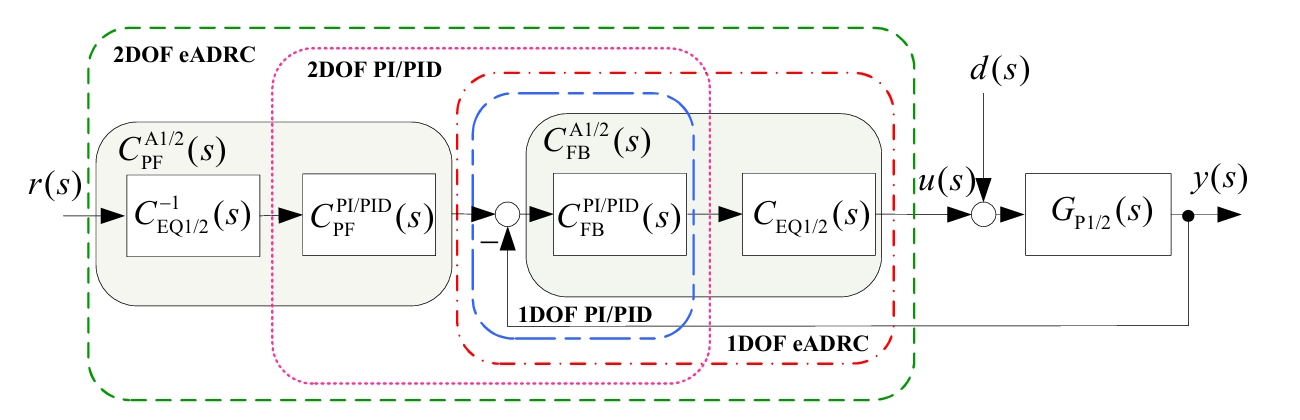
\includegraphics[width=0.95\linewidth]{pid2adrc.png}
    \caption[Equivalencias PID--eADRC]{Esquema de implementación de
    controladores PI/PID y eADRC en configuraciones 1DOF y 2DOF, y su
    equivalencia para plantas de orden relativo 1 y 2
    \cite{stankovic2024pid}.}
    \label{fig:pid2adrc}
\end{figure}

\textbf{ADRC basado en el error.} La mayoría de los algoritmos ADRC requieren
acceso independiente a $y$ y a $u$. Madoński et al. \cite{madonski2019general}
observan que muchos bloques de control comerciales tienen arquitectura cerrada
y solo aceptan el error $e=r-y$, y proponen el \emph{general error-based ADRC},
que reformula el ESO para depender exclusivamente del error de seguimiento.
Ese es el esquema que se implementa aquí, y es la razón por la que el bloque
resultante puede sustituir al PID existente sin recablear el lazo.

\textbf{Sintonía en el dominio de la frecuencia.} Cao et al.
\cite{cao2025cascaded} reinterpretan el ADRC como un PID precedido por filtros
en cascada (Figura~\ref{fig:casc}), lo que permite aplicar márgenes de ganancia
y de fase para ajustar sus parámetros y razonar sobre el compromiso entre
atenuación de ruido de sonda y velocidad de recuperación ante carga --- que en
este trabajo resulta ser, cuantitativamente, el compromiso que decide el
diseño.

\begin{figure}[H]
    \centering
    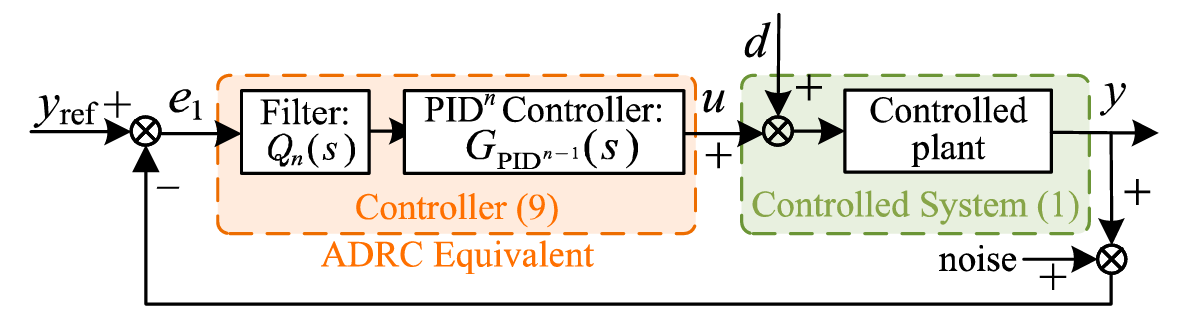
\includegraphics[width=0.72\linewidth]{casc.png}
    \caption[ADRC en forma de PID con filtro en cascada]{Esquema eADRC
    implementado en su forma equivalente de PID con filtro en cascada
    \cite{cao2025cascaded}.}
    \label{fig:casc}
\end{figure}

\subsection{Análisis comparativo}

La Tabla~\ref{tab:comparativa_control} sintetiza las fortalezas y debilidades
identificadas en la revisión, y fundamenta la elección del ADRC como estrategia
central.

\begin{table}[H]
\centering
\caption{Comparación técnica de estrategias de control para lodos activados.}
\label{tab:comparativa_control}
\renewcommand{\arraystretch}{1.35}
\small
\begin{tabular}{|p{2.1cm}|p{4.6cm}|p{4.9cm}|p{2.6cm}|}
\hline
\rowcolor[gray]{0.9}
\textbf{Estrategia} & \textbf{Ventajas} & \textbf{Limitaciones} & \textbf{Referencia} \\ \hline
\textbf{PID} & Estructura simple, bajo costo computacional, base instalada amplia. & No desacopla perturbaciones fuertes; compromiso entre rapidez y estabilidad; una sola sintonía para todo el rango de operación. & Iratni \& Chang \cite{iratni2019advances} \\ \hline
\textbf{MPC / NMPC} & Manejo explícito de restricciones y de sistemas multivariables. & Costo computacional elevado; sensible al error de modelo; mantenimiento difícil. & Li \& Yamamoto \cite{li2017multi} \\ \hline
\textbf{RN / Difuso} & Modela dinámicas complejas sin ecuaciones explícitas. & Estructura opaca; validación de estabilidad difícil; depende de datos de calidad. & Qiao et al. \cite{qiao2014neural} \\ \hline
\textbf{ADRC / GPI} & Estima y cancela la perturbación total; equilibrio entre desempeño y simplicidad; sintonía por ancho de banda. & Requiere diseño cuidadoso del observador ante ruido de medida; menor penetración comercial. & Wei et al. \cite{wei2020disturbance} \\ \hline
\end{tabular}
\end{table}

\subsection{Métricas de desempeño y robustez}
\label{subsec:metricas}

Para comparar los controladores a lo largo del documento se usan las métricas clásicas de desempeño y
de esfuerzo de control de la Tabla~\ref{tab:metricas}. Se miden desde el instante
$t_0$ del cambio de consigna o de la perturbación hasta el final de la ventana $t_f$, con el error de
seguimiento $e(t) = y(t) - r(t)$ y el tamaño del cambio de consigna $\Delta r$.

\begin{table}[H]
\centering
\caption{Métricas de desempeño y de esfuerzo de control usadas en el documento.}
\label{tab:metricas}
\small
\renewcommand{\arraystretch}{1.15}
\begin{tabular}{@{}l>{\centering\arraybackslash}p{6.0cm}>{\raggedright\arraybackslash}p{7.0cm}@{}}
\toprule
\textbf{Métrica} & \textbf{Definición} & \textbf{Qué mide} \\
\midrule
IAE & $\displaystyle\int_{t_0}^{t_f} |e(t)|\,dt$ & Error acumulado en la ventana. \\
$\overline{|e|}$ & $\dfrac{\mathrm{IAE}}{t_f - t_0}$ & Error absoluto medio; compara ventanas de distinta duración. \\
ITAE & $\displaystyle\int_{t_0}^{t_f} (t - t_0)\,|e(t)|\,dt$ & Error acumulado, pesando más el que tarda en desaparecer. \\
RMS & $\displaystyle\sqrt{\frac{1}{t_f - t_0}\int_{t_0}^{t_f} e^2(t)\,dt}$ & Error cuadrático medio. \\
$\max|e|$ & $\max_t\,|e(t)|$ & Mayor desviación; ante una perturbación, la caída máxima. \\
$M_p$ & $\dfrac{100\,\max_t\,\operatorname{sgn}(\Delta r)\,\bigl(y(t) - r\bigr)}{|\Delta r|}$ & Sobrepico, en \% del cambio de consigna; ante una perturbación, en \% de la caída máxima. \\
$t_s$ & menor $t_s$ con $|e(t)| \le 0{,}02\,|\Delta r|$ para todo $t \ge t_0 + t_s$ & Tiempo de asentamiento, con banda de $2~\%$ del cambio. \\
\midrule
$u_{\max}$, $u_{\min}$ & $\max_t\,u(t)$, \ $\min_t\,u(t)$ & Valores extremos de la señal de control. \\
$E_u$ & $\displaystyle\int_{t_0}^{t_f} \bigl(u(t) - u_\infty\bigr)^2\,dt$ & Energía de la señal de control respecto a su valor final. \\
TV & $\displaystyle\sum_k \bigl|u[k] - u[k-1]\bigr|$ & Variación total, el recorrido del actuador; TV/h, por hora. \\
$\sigma_u$ & $\operatorname{std}\bigl(u_{\text{con ruido}} - u_{\text{sin ruido}}\bigr)$ en estacionario & Ruido del sensor que llega a la señal de control. \\
$\sigma_{\Delta u}/\sqrt{2}$ & $\operatorname{std}\bigl(u[k] - u[k-1]\bigr)/\sqrt{2}$ & Movimiento de $u$ de una muestra a la siguiente. \\
\bottomrule
\end{tabular}
\end{table}

Para la robustez se usan las métricas clásicas de la Tabla~\ref{tab:metricas_robustez}, calculadas
sobre el lazo abierto $G_L(s) = C(s)\,G(s)$, con la planta $G(s)$ y el controlador $C(s)$;
$\omega_{gc}$ es el cruce de ganancia y $\omega_{pc}$, el cruce de fase.

\begin{table}[H]
\centering
\caption{Métricas de robustez usadas en el documento.}
\label{tab:metricas_robustez}
\small
\renewcommand{\arraystretch}{1.3}
\begin{tabular}{@{}l>{\centering\arraybackslash}p{6.0cm}>{\raggedright\arraybackslash}p{7.0cm}@{}}
\toprule
\textbf{Métrica} & \textbf{Definición} & \textbf{Qué mide} \\
\midrule
MF & $180^{\circ} + \angle G_L(j\omega_{gc})$, \newline con $|G_L(j\omega_{gc})| = 1$ & Margen de fase: la fase que puede perder el lazo antes de volverse inestable. \\
MG & $1/|G_L(j\omega_{pc})|$, \newline con $\angle G_L(j\omega_{pc}) = -180^{\circ}$ & Margen de ganancia: cuánto puede crecer la ganancia del lazo. \\
$\theta_{\max}$ & $\dfrac{\pi}{180^{\circ}}\,\dfrac{\mathrm{MF}}{\omega_{gc}}$ & Retardo máximo que aguanta el lazo. \\
$M_s$ & $\max_{\omega}\,|S(j\omega)|$, \newline con $S(s) = 1/\bigl(1 + G_L(s)\bigr)$ & Pico de la sensibilidad; entre más bajo, más robusto. \\
$M_t$ & $\max_{\omega}\,|T(j\omega)|$, \newline con $T(s) = G_L(s)/\bigl(1 + G_L(s)\bigr)$ & Pico de la sensibilidad complementaria; resonancia del lazo cerrado. \\
$\omega_{BW}$ & $|T(j\omega)| < 1/\sqrt{2}$ para $\omega > \omega_{BW}$ & Ancho de banda del lazo cerrado ($-3$~dB); qué tan rápido es el lazo. \\
\bottomrule
\end{tabular}
\end{table}

\section{Planteamiento del problema}
\label{sec:problema}

En la industria, la mayoría de los lazos de control se siguen cerrando con
controladores PID sintonizados de forma empírica, que al ser lineales y de
parámetros fijos solo quedan bien ajustados para un punto de operación. Esto
se vuelve una limitación en procesos no lineales, con múltiples perturbaciones
asociadas y múltiples incertidumbres, en los que se plantea la necesidad de un
cambio de paradigma: buscar nuevos controladores que dejen de lado el PID y
compitan directamente con él, en vista de una mejora en el desempeño y de un
avance tecnológico. El ADRC ofrece esa posibilidad, ya que permite implementar
un controlador lineal sobre un sistema no lineal, agrupando las perturbaciones
y las incertidumbres en una sola señal que se estima y se cancela en línea.

Ahora bien, un caso donde este paradigma puede implementarse es el lazo de
oxígeno disuelto en la etapa de lodos activados de una PTAR. Este proceso es
no lineal, incierto en algunos parámetros y está sometido a perturbaciones como el caudal de entrada, la carga
orgánica, la activación de sopladores y el ruido en las señales de medida, y
debe mantenerse en un rango de operación de 1,5 a 2,5~mg/L. Por ende, un PID
convencional ISA sintonizado empíricamente puede resultar en una regulación
imprecisa del OD y un consumo energético
ineficiente.  Es
decir, el problema no es solo mejorar la regulación del OD, sino demostrar que
algoritmos de control más avanzados pueden implementarse en un PLC, competir
directamente contra el PID y ofrecer algunas ventajas dadas por su estructura,
su forma de sintonización y su funcionamiento.


\section{Objetivos}
\label{sec:objetivos}

\subsection{Objetivo general}

Comparar dos estrategias de control basadas en rechazo activo de
perturbaciones para la regulación del oxígeno disuelto en la etapa de lodos
activados de una planta de tratamiento de aguas residuales, con el fin de
mejorar el desempeño frente a perturbaciones operativas como el caudal de
entrada, el ruido de los sensores de oxígeno, la activación de aireadores
auxiliares, y las asociadas a variaciones en la carga orgánica y en los
parámetros químicos del afluente.

\subsection{Objetivos específicos}

\begin{itemize}
  \item[\textbf{OE1}] Caracterizar las perturbaciones que afectan el sistema de
  dosificación de oxígeno en la etapa de lodos activados, con el propósito de
  apoyar el diseño y la evaluación de los controladores basados en rechazo
  activo de perturbaciones.
  \item[\textbf{OE2}] Diseñar un primer controlador proporcional-integral
  generalizado (GPI) robusto basado en el error de seguimiento para el proceso
  de dosificación de oxígeno.
  \item[\textbf{OE3}] Diseñar un segundo controlador con rechazo activo de
  perturbaciones basado en observador de estado extendido (ESO) enfocado en el
  error de seguimiento.
  \item[\textbf{OE4}] Desarrollar una metodología para la implementación de
  controladores basados en rechazo activo de perturbaciones en entornos
  industriales mediante PLC, considerando aspectos prácticos como el manejo de
  saturación y la facilidad de implementación.
  \item[\textbf{OE5}] Validar experimentalmente los controladores propuestos
  frente a un PID convencional, empleando métricas clásicas de desempeño y
  robustez.
\end{itemize}


\section{Metodología}
\label{sec:metodologia}

El trabajo se desarrolló en seis fases, cada una asociada a uno o varios capítulos del documento
y a los objetivos específicos (Tabla~\ref{tab:metodologia}).

\begin{table}[H]
\centering
\caption{Resumen de la metodología del trabajo.}
\label{tab:metodologia}
\renewcommand{\arraystretch}{1.08}
\small
\begin{tabular}{|p{1.2cm}|>{\raggedright\arraybackslash}p{2.9cm}|>{\raggedright\arraybackslash}p{10.1cm}|}
\hline
\rowcolor[gray]{0.9}
\textbf{Fase} & \textbf{Etapa} & \textbf{Descripción} \\ \hline
\textbf{Fase 1} & Revisión y caracterización (Cap.~\ref{cap:introduccion} y~\ref{cap:caracterizacion}; OE1) &
\textbullet~Estado del arte del control de OD, del ADRC y del GPI.\newline
\textbullet~Análisis de los datos de operación: régimen diario, lazo con el PID, escalones del soplador y caudales.\newline
\textbullet~Perturbación total reconstruida de los datos, su espectro y el ruido del sensor. \\ \hline
\textbf{Fase 2} & Modelado (Cap.~\ref{cap:caracterizacion}) &
\textbullet~Modelo de primer orden con retardo identificado de los escalones, con sus rangos de variación.\newline
\textbullet~Validación con los datos, planta nominal y ganancia $b_0$. \\ \hline
\textbf{Fase 3} & Diseño de controladores (Cap.~\ref{cap:ADRC-ESO} y~\ref{cap:GPI}; OE2 y OE3) &
\textbullet~ADRC con ESO basado en el error de seguimiento, con sintonía por anchos de banda.\newline
\textbullet~GPI con integradores y su equivalencia con el ADRC con ESO.\newline
\textbullet~Análisis de robustez y ante variaciones de la planta, en Python y Simulink. \\ \hline
\textbf{Fase 4} & Implementación en PLC (Cap.~\ref{cap:implementacion}; OE4) &
\textbullet~Saturación, acondicionamiento de la referencia, ruido y retardo.\newline
\textbullet~Discretización y realización con retardos.\newline
\textbullet~Bloques de función en texto estructurado, probados en el PLC con una planta simulada. \\ \hline
\textbf{Fase 5} & Validación (Cap.~\ref{cap:comparacion_pid}; OE5) &
\textbullet~Simulación contra un PID ISA de igual robustez: consigna, retardo, ruido y perturbación reconstruida.\newline
\textbullet~Métricas de desempeño (IAE, ITAE, sobrepico, tiempo de asentamiento) y de esfuerzo de control. \\ \hline
\textbf{Fase 6} & Análisis y documentación (Cap.~\ref{cap:discusion} y~\ref{cap:conclusiones}) &
\textbullet~Discusión de resultados, limitaciones e implicaciones prácticas.\newline
\textbullet~Recetas de implementación y redacción del documento. \\ \hline
\end{tabular}
\end{table}




% ============================================================================
%  Capítulo 3 — Caracterización
% ============================================================================
\chapter{Caracterización y modelado de la planta}


\label{cap:caracterizacion}

Este capítulo busca encontrar el modelo representativo de la dinámica de la
planta, junto con sus parámetros (la constante de tiempo $\tau$, la ganancia
$K$ y el retardo $\theta$), e identificar algunas de las perturbaciones que
afectan el lazo de control de oxígeno disuelto. Para ello se parte de un P\&ID
del proceso de aireación en la etapa de lodos activados, con el fin de obtener
la ecuación que explica la dinámica del sistema y encontrar una forma
simplificada que permita la implementación del controlador ADRC.

Ahora bien, para encontrar los parámetros se analizan los datos de la planta:
el histórico medido durante un periodo de 22 meses y almacenado en el sistema
SCADA. Por ende, el capítulo se divide así: el P\&ID del proceso y del lazo de
control; el modelo dinámico y su forma simplificada para el ADRC; el
comportamiento actual del lazo con el PID; los escalones de soplador en lazo
abierto y el ensayo hecho directamente en el PLC, con el que se mide el
retardo; la identificación de $\tau$ y $K$ por ventanas ARX y su validación; el ruido
del sensor; el perfil diario de los
caudales; la reconstrucción de la perturbación total; su espectro; y, al final,
un resumen de todos los parámetros identificados.

\section{P\&ID y lazo de control de la planta}
\label{sec:pid_planta}

Para entender fácilmente los componentes y los equipos que hacen parte del
proceso de aireación, se elaboró un diagrama P\&ID siguiendo la norma ISA-5.1
(Figura~\ref{fig:pid_tikz}). En él, el lazo 100 es el de oxígeno disuelto, que es
el de interés para este trabajo, y los lazos 101 y 102 miden los caudales. Es importante mencionar que la planta
tiene tres módulos idénticos (M1, M2 y M3), que realizan esta misma tarea en
tres áreas diferentes de la planta. A continuación se describe cada etapa del
proceso y los componentes de cada lazo.


\begin{figure}[H]
    \centering
    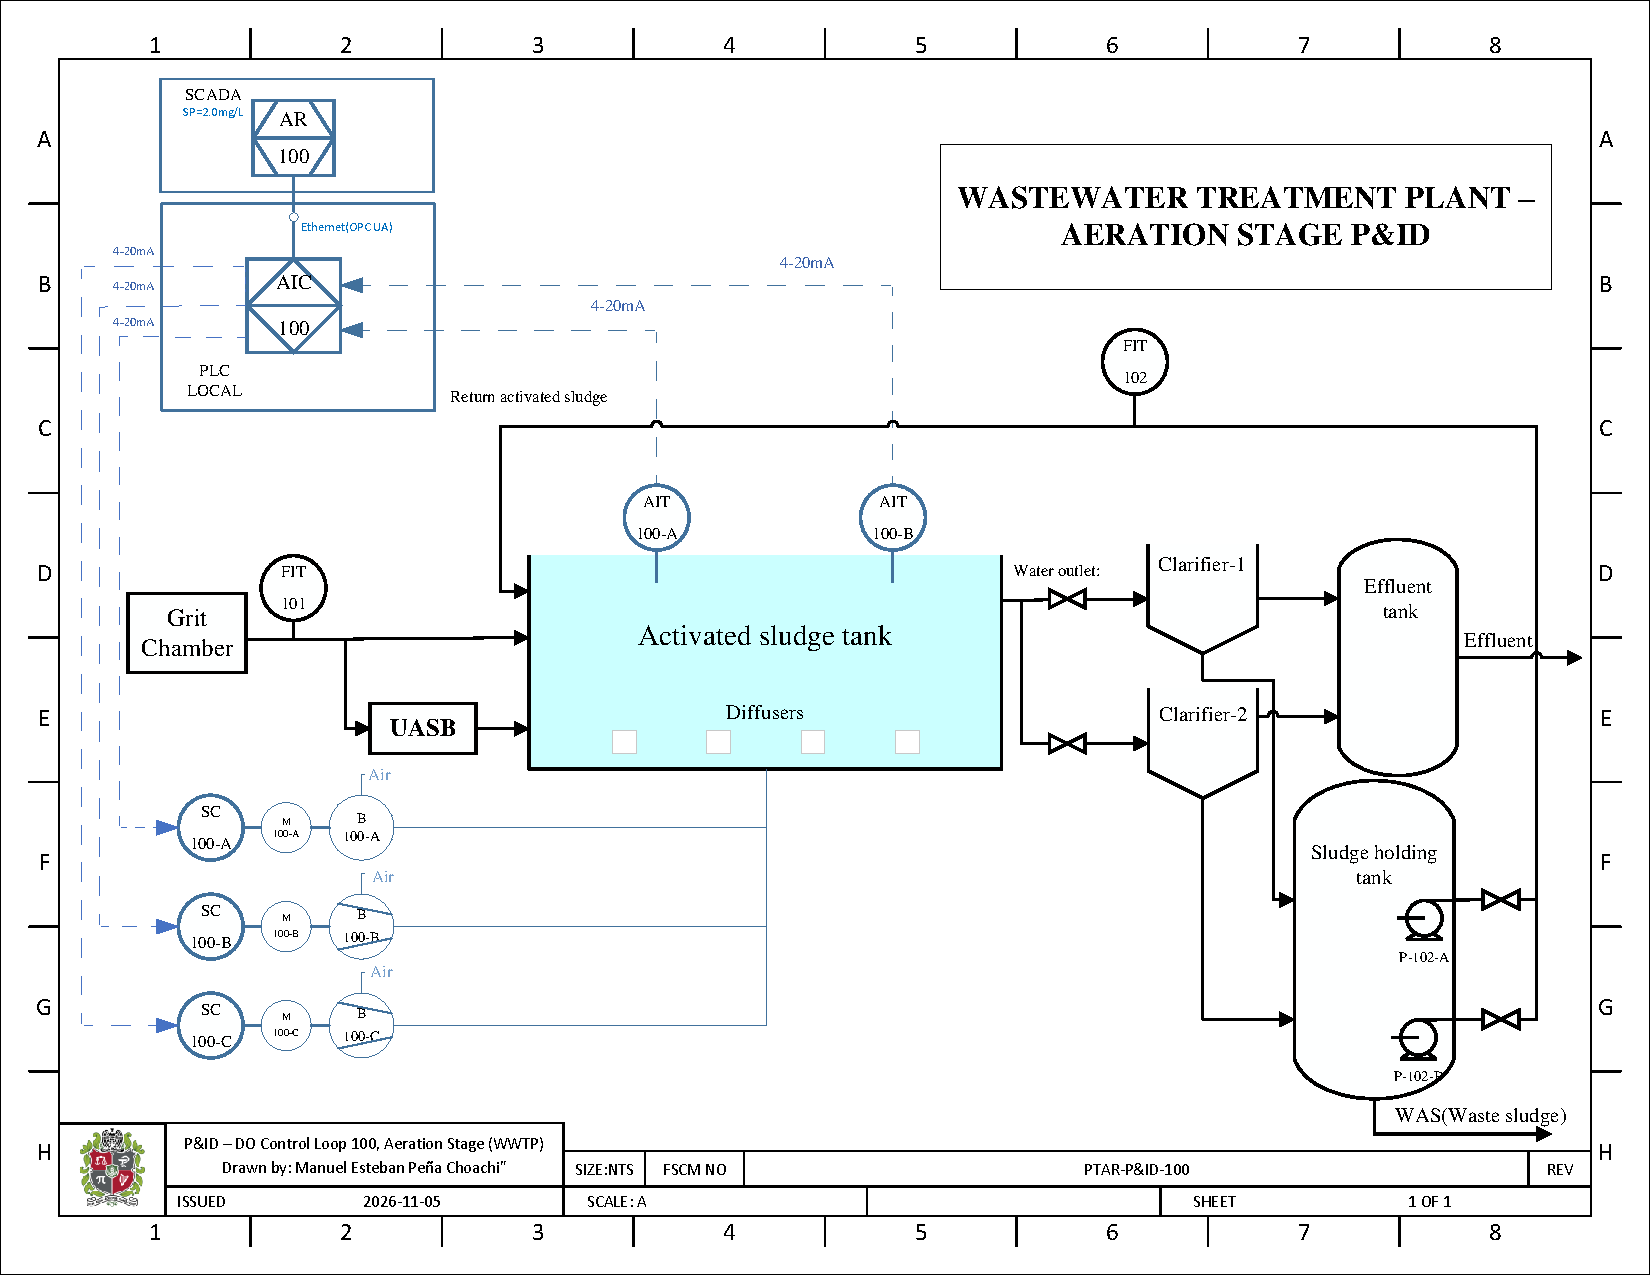
\includegraphics[width=\textwidth]{pid_ptar.pdf}
    \caption[P\&ID simplificado de la etapa de aireación]{P\&ID simplificado de la
    etapa de aireación según la simbología ISA-5.1. El agua del desarenador
    (FIT-101) llega al tanque de aireación directamente y a través del UASB; sale a
    los sedimentadores secundarios, y el lodo vuelve al tanque como recirculación
    (FIT-102). En el lazo 100, los dos transmisores de oxígeno (AIT-100-A y AIT-100-B)
    llegan al controlador AIC-100 del PLC local, que fija la velocidad de los
    variadores (SC-100-A/B/C) de los sopladores; el SCADA (AR-100) registra el OD y le
    envía la consigna al PLC por Ethernet.}
    \label{fig:pid_tikz}
\end{figure}

\subsection*{Etapas del proceso}

\begin{itemize}
  \item \textbf{Pretratamiento y desarenador.} El caudal de entrada pasa por
  rejillas y filtros continuos, que retiran los elementos más pesados, y por
  los desarenadores, que separan el líquido de la arena y otros sólidos.

  \item \textbf{Reparto del caudal.} A la salida del desarenador el caudal se
  divide en dos líneas: una va directamente al tanque de aireación y la
  otra al UASB.

  \item \textbf{UASB} (\emph{Upflow Anaerobic Sludge Blanket}). Es un reactor
  anaerobio que degrada la materia orgánica y produce biogás. De él salen tres
  corrientes: el biogás, un flujo líquido que entra al tanque de aireación (sin
  transmisor que lo mida) y un flujo sólido que va al tanque de lodos.

  \item \textbf{Tanque de aireación.} Es el reactor de lodos activados,
  donde la biomasa aerobia degrada la materia orgánica con el oxígeno que
  entregan los difusores ubicados en el fondo.

  \item \textbf{Sedimentadores o clarificadores.} Reciben la mezcla del
  tanque de aireación y separan el agua tratada de la biomasa, que se acumula
  en el fondo y se envía al tanque de lodos. El agua tratada se almacena y sale
  como efluente.


  \item \textbf{Recirculación de lodos (RAS).} Parte del lodo vuelve desde el
  tanque de lodos al tanque de aireación para mantener la concentración de
  biomasa.
\end{itemize}

\subsection*{Lazo 100: control de oxígeno disuelto}

Ahora bien, el lazo más importante es el 100, que constituye el control de
oxígeno disuelto. Sus componentes, en el orden en que viaja la señal, son:

\begin{itemize}
  \item \textbf{Transmisores de oxígeno AIT-100-A y AIT-100-B.} Miden la
  variable del proceso, es decir, el oxígeno disuelto a la entrada y a la
  salida del tanque de aireación, y envían una señal de 4--20~mA al PLC local.

  \item \textbf{PLC local (AIC-100).} Está en un tablero en campo, cerca del proceso.
  Convierte las señales de 4--20~mA a mg/L según la hoja técnica de los
  transmisores y calcula el promedio de las dos medidas de oxígeno. Seguido a
  esto, el controlador AIC-100 compara ese promedio con la referencia de 2,0~mg/L y
  calcula la señal de control $u$, que dentro del PLC se maneja como una
  consigna de 0 a 100~\% y se traduce a una señal de 4--20~mA para los
  variadores.

  \item \textbf{SCADA (AR-100).} Registra el oxígeno disuelto y, desde él, el
  operador cambia la consigna, que llega al PLC por Ethernet.

  \item \textbf{Variadores SC-100-A/B/C.} Reciben la señal de control como
  4--20~mA y fijan la velocidad de los motores.

  \item \textbf{Sopladores B-100-A/B/C.} Accionados por sus motores, envían
  el aire de proceso.

  \item \textbf{Difusores.} Distribuyen el aire en el fondo del tanque de
  aireación, donde el oxígeno se transfiere al agua y cierra el lazo sobre la
  medida de los AIT.
\end{itemize}

La Figura~\ref{fig:lazo100_bloques} muestra el mismo lazo en bloques, en el orden en que
viaja la señal, antes de escribir cada bloque como una función de transferencia (Sección~\ref{sec:car_modelo}).

\begin{figure}[H]
    \centering
    \resizebox{\textwidth}{!}{%
    \begin{tikzpicture}[>=Stealth, thick, font=\small,
        blq/.style={draw, thick, fill=white, align=center, minimum height=1.15cm, inner sep=4pt},
        suma/.style={draw, thick, circle, fill=white, minimum size=0.5cm, inner sep=0pt}]
        % ---- PLC local: controlador y promedio ----
        \draw[thin, dashed, gray!70!black, rounded corners=3pt] (1.1,-3.25) rectangle (3.7,1.05);
        \node[font=\footnotesize, gray!40!black, anchor=north west] at (1.15,1.02) {PLC local};
        % ---- camino directo: controlador, actuador y planta ----
        \node[suma] (s) at (0,0) {};
        \node[blq] (aic) at (2.4,0) {Controlador\\AIC-100};
        \node[blq] (sc) at (7.0,0) {Variadores\\SC-100-A/B/C};
        \node[blq] (sop) at (11.0,0) {Motores y\\sopladores};
        \node[blq] (dif) at (13.9,0) {Difusores};
        \node[blq, fill=cyan!8] (tq) at (17.2,0) {Tanque de\\aireación};
        \draw[->] (-1.6,0) -- node[above, align=center, font=\footnotesize] {consigna $r$\\(SCADA)} (s.west);
        \draw[->] (s.east) -- node[above, font=\footnotesize] {error} (aic.west);
        \draw[->] (aic.east) -- node[above, font=\footnotesize, pos=0.6] {$u$ [\%]} node[below, font=\footnotesize, pos=0.6] {4--20 mA} (sc.west);
        \draw[->] (sc.east) -- node[above, font=\footnotesize] {velocidad} (sop.west);
        \draw[->] (sop.east) -- node[above, font=\footnotesize] {aire} (dif.west);
        \draw[->] (dif.east) -- node[above, font=\footnotesize] {oxígeno} (tq.west);
        \draw[->] (17.2,1.6) node[above, font=\footnotesize] {perturbaciones: caudales y carga} -- (tq.north);
        \draw[->] (tq.east) -- (19.9,0) node[above left, font=\footnotesize] {OD};
        \fill (19.2,0) circle (2pt);
        % ---- realimentacion: medida ----
        \node[blq] (ait) at (13.6,-2.4) {Transmisores\\AIT-100-A y AIT-100-B};
        \node[blq] (prom) at (2.4,-2.4) {Promedio de\\los sensores};
        \draw[->] (19.2,0) -- (19.2,-2.4) -- (ait.east);
        \draw[->] (13.6,-3.75) node[below, font=\footnotesize] {ruido de medida} -- (ait.south);
        \draw[->] (ait.west) -- node[above, font=\footnotesize] {4--20 mA} (prom.east);
        \draw[->] (prom.west) -- (0,-2.4) -- node[left, font=\footnotesize, pos=0.5] {OD medido $y$} (s.south);
        \node[font=\footnotesize] at ($(s.west)+(-0.2,-0.28)$) {$+$};
        \node[font=\footnotesize] at ($(s.south)+(0.28,-0.22)$) {$-$};
    \end{tikzpicture}}
    \caption[Lazo de control 100 en bloques]{Lazo de control 100 en diagrama de bloques: la
    consigna del SCADA entra al controlador AIC-100 del PLC local, que fija la velocidad de los
    variadores; los sopladores mandan el aire a los difusores y el oxígeno entra a la planta, el tanque de
    aireación, donde actúan las perturbaciones. Los dos transmisores cierran el lazo con el promedio
    del OD medido.}
    \label{fig:lazo100_bloques}
\end{figure}

\subsection*{Lazos 101 y 102: caudales}

Al tanque de aireación llegan tres caudales: el directo del desarenador, el que
sale del UASB y la recirculación de lodos. Estos lazos solo miden los flujos de
líquido que entran al tanque, de modo que desde el punto de vista del control se
pueden ver como perturbaciones. Todos los caudales de la planta se registran en L/s.

\begin{itemize}
  \item \textbf{FIT-101.} Transmisor indicador de caudal a la salida del
  desarenador. Mide el caudal total antes del reparto.
  \item \textbf{FIT-102.} Transmisor indicador del caudal de recirculación de
  lodos (caudalímetro de 12~in), que mueven las bombas P-102-A y P-102-B.
  \item \textbf{Flujo del UASB.} No tiene transmisor, por lo que no se mide.
\end{itemize}


\section{Modelo dinámico}
\label{sec:car_modelo}

El modelo parte de un balance de masa de oxígeno disuelto sobre el tanque de
aireación, considerado como un reactor de mezcla completa. Se utilizaron como
guía las ecuaciones del BSM1 \cite{alex2008bsm1} y del ASM1
\cite{henze1987asm1}, adaptando las unidades a las que manejan los operarios de
la planta; en particular, el tiempo se expresa en horas, mientras que en el
BSM1 está en días.

\begin{equation}
\text{Acumulación}=\text{Entrada}-\text{Salida}+\text{Generación}-\text{Consumo}.
\end{equation}

Al tanque entran los tres caudales identificados en el P\&ID: el directo del
desarenador, el que sale del UASB y la recirculación de lodos ($i=1,2,3$). La
generación es la transferencia de oxígeno de los difusores, y el consumo es la
respiración de la biomasa. Así, el balance queda de la siguiente forma:

\begin{equation}
\frac{dS_O}{dt}=\frac{1}{V}\sum_{i=1}^3 Q_{in,i}\,S_{O_{in,i}}
-\frac{Q_{out}}{V}\,S_O+K_{La}\left(S^{*}_O-S_O\right)-r_z(S_O),
\label{eq:car_balance}
\end{equation}

y cada término tiene unidades de concentración por unidad de tiempo:

\begin{equation}
\underbrace{\frac{dS_O}{dt}}_{\frac{\mathrm{mg}}{\mathrm{L}\cdot\mathrm{h}}}
=
\underbrace{\frac{1}{V}\sum_{i=1}^3 Q_{in,i}S_{O_{in,i}}}_{\frac{1}{\mathrm{L}}
\left(\frac{\mathrm{L}}{\mathrm{h}}\right)
\left(\frac{\mathrm{mg}}{\mathrm{L}}\right)
=
\frac{\mathrm{mg}}{\mathrm{L}\cdot\mathrm{h}}}
-
\underbrace{\frac{Q_{out}}{V}S_O}_{\left(\frac{\mathrm{L}/\mathrm{h}}{\mathrm{L}}\right)
\left(\frac{\mathrm{mg}}{\mathrm{L}}\right)
=
\frac{\mathrm{mg}}{\mathrm{L}\cdot\mathrm{h}}}
+
\underbrace{K_{La}(S^{*}_O-S_O)}_{\left(\frac{1}{\mathrm{h}}\right)
\left(\frac{\mathrm{mg}}{\mathrm{L}}\right)
=
\frac{\mathrm{mg}}{\mathrm{L}\cdot\mathrm{h}}}
-
\underbrace{r_z(S_O)}_{\frac{\mathrm{mg}}{\mathrm{L}\cdot\mathrm{h}}}.
\label{ecu:nonlineal}
\end{equation}

El consumo de oxígeno $r_z$ se toma del ASM1, como en el
BSM1, y corresponde al crecimiento aerobio de la biomasa heterótrofa
($\rho_1$) y autótrofa ($\rho_3$):

\begin{equation}
    r_{z} = \frac{1 - Y_H}{Y_H}\,\rho_1 + \frac{4{,}57 - Y_A}{Y_A}\,\rho_3 ,
    \label{eq:car_rz}
\end{equation}

\begin{equation}
    \rho_1 = \mu_H \left(\frac{S_S}{K_S + S_S}\right)\left(\frac{S_O}{K_{O,H} + S_O}\right) X_{B,H},
\end{equation}

\begin{equation}
    \rho_3 = \mu_A \left(\frac{S_{NH}}{K_{NH} + S_{NH}}\right)\left(\frac{S_O}{K_{O,A} + S_O}\right) X_{B,A}.
\end{equation}


Ahora bien, la variable que realmente se manipula no es $K_{La}$ sino la
consigna $u$ que el PLC envía a los variadores. Si se considera que el
coeficiente de transferencia es proporcional a esa señal, quedaría de la
siguiente forma:

\begin{equation}
K_{La} = k_\alpha\, u , \qquad u \in [0,100]~\%,
\end{equation}

donde $k_\alpha$ es una constante de proporcionalidad que, en el rango de
operación, se puede estimar como

\begin{equation}
k_\alpha = \frac{K_{La_{max}}-K_{La_{min}}}{100-0},
\qquad
\left[k_\alpha\right] = \left[\frac{\mathrm{h}^{-1}}{\%}\right].
\end{equation}

Esta ganancia agrupa toda la cadena de actuación, desde la señal del PLC hasta
la transferencia de oxígeno en los difusores, como se descompone en la
Tabla~\ref{tab:gain_decomposition}. Se aclara que esta relación es solo una
aproximación, y se utiliza para entender las suposiciones del modelo
simplificado y las discrepancias que van a existir entre este y el
comportamiento real de la planta.

\begin{table}[H]
\centering
\caption{Descomposición de la ganancia $k_\alpha$ a lo largo de la cadena de
actuación.}
\label{tab:gain_decomposition}
\begin{tabular}{cll}
\toprule
\textbf{Etapa} & \textbf{Conversión} & \textbf{Ganancia} \\
\midrule
1. PLC          & 0--100~\% $\to$ 4--20\,mA          & $k_{\mathrm{PLC}} = 0{,}16$\,mA/\% \\
2. Variador / motor  & 4--20\,mA $\to$ 0--3000\,rpm  & $k_{\mathrm{VFD}} = 187{,}5$\,rpm/mA \\
3. Soplador     & $n \to Q_{\mathrm{aire}}$            & $k_Q = Q_{\mathrm{aire}}^{\max}/n^{\max}$ \\
4. Aireación    & $Q_{\mathrm{aire}} \to K_{La}$      & $k_{K_{La}}$ \\
\midrule[\heavyrulewidth]
\multicolumn{2}{l}{\textbf{Ganancia total} $k_\alpha = K_{La}/u$}
                & $k_\alpha = k_{K_{La}}\, k_Q\, k_{\mathrm{VFD}}\, k_{\mathrm{PLC}}$ \\
\bottomrule
\end{tabular}
\end{table}

Sustituyendo $K_{La}=k_\alpha u$ en el balance \eqref{eq:car_balance}, la
dinámica queda en forma afín respecto a la entrada $u$:

\begin{equation}
\dot S_O
=
\underbrace{
\frac{1}{V}\sum_{i=1}^3 Q_{in,i}S_{O_{in,i}}
-\frac{Q_{out}}{V}S_O
-r_z(S_O)
}_{f(S_O,t)}
+
u\,
\underbrace{
k_\alpha\left(S^{*}_O-S_O\right)
}_{g(S_O,t)},
\end{equation}

es decir,

\begin{equation}
\dot S_O = f(S_O,t) + g(S_O,t)\,u .
\label{eq:car_afin}
\end{equation}

Por ende, el sistema no es lineal: la ganancia de entrada $g$ depende del
propio oxígeno disuelto; es decir, la entrada $u$ aparece multiplicada por
una variable de estado del sistema. Este tipo de problema entra en el campo de
los sistemas no lineales, y si bien se podría resolver con técnicas más
complejas, como la teoría de planitud diferencial, encontrando una salida
plana que parametrice las variables del sistema (si se tuviera la suerte de que existiera), en este caso se optó por
validar un enfoque al estilo del ADRC. Este consiste en agrupar toda la
dinámica que difiere de un integrador puro dentro de una perturbación total
$\bar{\xi}$, y dejar fuera solo una ganancia de entrada constante $\overline{b_0}$:

\begin{equation}
    \dot{y} = \bar{\xi} + \overline{b_0}\, K_{La},
\end{equation}

Ahora bien, si se agrega el término $\overline{b_0}\, K_{La}$, es necesario
restarlo dentro de la perturbación total para que la ecuación no cambie,
quedando de la siguiente forma:

\begin{equation}
\bar{\xi}
=
\frac{1}{V}\sum_{i=1}^3 Q_{in,i}S_{O_{in,i}}
-\frac{Q_{out}}{V}S_O
-r_z(S_O)+K_{La}\left(S^{*}_O-S_O\right)-\overline{b_0}\, K_{La}.
\end{equation}

Sustituyendo de nuevo $K_{La} = k_\alpha u$:


\begin{equation}
\bar{\xi}
=
\frac{1}{V}\sum_{i=1}^3 Q_{in,i}S_{O_{in,i}}
-\frac{Q_{out}}{V}S_O
-r_z(S_O)
+ {\color{red}{k_\alpha u}} \left(S^{*}_O-S_O\right)
-\overline{b_0}\, {\color{red}{k_\alpha u}},
\label{ecu:disturbance}
\end{equation}

y definiendo $b_0 = \overline{b_0}\, k_\alpha$, con unidades

\begin{equation}
\left[b_0\right]=\left[\frac{\mathrm{mg}}{\mathrm{L}}\right] \cdot \left[\frac{\mathrm{h}^{-1}}{\%}\right]
= \left[\frac{\mathrm{mg}}{\mathrm{L}\cdot\mathrm{h}\cdot\%}\right],
\end{equation}

se llega a la forma canónica del ADRC de primer orden, en la que cada término
tiene unidades consistentes para este sistema:

\begin{equation}
\underbrace{\dot{y}}_{\left[\frac{\mathrm{mg}}{\mathrm{L}\cdot\mathrm{h}}\right]}
=
\underbrace{\bar{\xi}}_{\left[\frac{\mathrm{mg}}{\mathrm{L}\cdot\mathrm{h}}\right]}
+
\underbrace{b_0}_{\left[\frac{\mathrm{mg}}{\mathrm{L}\cdot\mathrm{h}\cdot\%}\right]}
\cdot
\underbrace{u}_{[\%]} .
\label{eq:car_canonica}
\end{equation}

Ahora bien, en la práctica $b_0$ no se calcula a partir de los parámetros del
ASM1, que no se miden en la planta, sino que se obtiene de un modelo de primer
orden identificado con los datos. Ese modelo, con retardo $\theta$, es

\begin{equation}
G(s)=\frac{Y(s)}{U(s)}
=
\frac{k_{dc}}{\tau s+1}\,e^{-\theta s}.
\label{eq:car_foptd}
\end{equation}

Para el desarrollo que sigue se toma $\theta=0$, lo que simplifica el diseño
y permite ver con claridad la relación entre la planta y la perturbación total.
La simplificación es razonable porque el retardo, que se acota entre 0 y
60~s (Sección~\ref{sec:ident_retardo}), es pequeño frente a la constante de
tiempo, $\theta/\tau \leq 0{,}06$; su efecto se retoma al acotar el ancho
de banda del observador. Llevando \eqref{eq:car_foptd}
a una cadena de integradores,

\begin{equation*}
s\,Y(s)=-\frac{Y(s)}{\tau}+\frac{k_{dc}}{\tau}\,U(s)
\qquad\Longrightarrow\qquad
\dot{y}(t)=-\frac{y(t)}{\tau}+\frac{k_{dc}}{\tau}\,u(t),
\end{equation*}

y agrupando el polo propio de la planta dentro de la perturbación total,

\begin{equation*}
\dot{y}(t)=\bar{\xi}(t) + \frac{k_{dc}}{\tau}\,u(t),
\qquad \bar{\xi}(t)  \leftarrow -\frac{y(t)}{\tau}.
\end{equation*}

Por ende, la ganancia de entrada que necesita el ADRC queda determinada por los
dos parámetros que se identifican en la planta,

\begin{equation}
b_0=\frac{k_{dc}}{\tau},
\qquad
\dot{y}(t)=\bar{\xi}(t) + b_0\, u(t),
\label{eq:car_b0}
\end{equation}

que es precisamente la forma del ADRC \eqref{eq:car_canonica}. En este caso,
la perturbación total abarca todos los términos mostrados en la
ecuación~\eqref{ecu:disturbance}: los caudales de entrada y de salida (es
importante mencionar que el caudal de salida se mantiene igual al de entrada,
de modo que el volumen del tanque es constante), la parte de la dinámica que
depende de la entrada y que no queda en $b_0$, el consumo de oxígeno por la
respiración biológica y las incertidumbres propias de algunos parámetros de la
planta. Las secciones siguientes se dedican a estimar $k_{dc}$, $\tau$ y
$\theta$ a partir del histórico de la planta, para obtener la ganancia $b_0$,
estimar la perturbación total y cuantificar el efecto que tiene cada
perturbación en la señal de control.

% ============================================================================
%  Caracterización a partir de los datos de planta
%  Figuras: figuras/ident_*.pdf, exportadas de
%  Datos/analisis/analisis_dinamica_limpio.ipynb
% ============================================================================
\section{Caracterización a partir de los datos de planta}
\label{sec:ident}

Esta sección reúne la caracterización del lazo de oxígeno hecha sobre los datos
reales de la PTAR. Hay dos fuentes. La primera es el historiador del SCADA, que
guarda el oxígeno disuelto (OD) cada minuto en los tres módulos, la potencia
eléctrica del tablero de aireación cada minuto en M2 y M3, y los caudales,
niveles y presiones cada hora. La segunda son las trazas del PLC ctrlX de M1,
muestreadas a 50~ms, que son el único registro donde aparece directamente la
consigna $u$ que el PLC manda al variador.

Por eso, de cada módulo se toma lo que sus datos permiten. M1 no tiene medidor
de potencia, pero tiene el ensayo del 12 de marzo de 2026 registrado en el PLC
a 50~ms, con la consigna $u$ medida directamente; de él salen el retardo, el
ruido del sensor y la comparación entre el SCADA y el PLC. M2 y M3 tienen
medida de potencia, pero no de la consigna $u$; con ellos se hacen la
identificación por ventanas ARX, los caudales y la perturbación total. Como los tres módulos son idénticos en
proceso y en equipos, lo medido en M1 (por ejemplo, el retardo) se asume válido
para M2 y M3. Además, en M2 y M3 la potencia expresada en porcentaje de plena carga
se toma como si fuera la misma consigna $u$ en porcentaje; la diferencia entre
las dos, debida a la cadena variador--motor--soplador, queda incluida en la
perturbación total (Sección~\ref{sec:ident_arx}).

% ----------------------------------------------------------------------------
\subsection{Línea temporal: el régimen de operación día a día}
\label{sec:ident_mapa}

Para saber qué datos se pueden utilizar para entender el sistema, cada día de
cada módulo se clasificó como PID en automático o manual. La clasificación se
hace a partir del error de seguimiento y de cuántas veces el OD cruza la
referencia, de cuánto se aleja el OD por encima de ella y de si el soplador
modula o está fijo. Los días con el sensor congelado se marcan aparte.

La Figura~\ref{fig:ident_mapa} muestra el resultado. Ahora bien, los
días manuales son los que se usan para identificar la planta, y los de PID para
medir el desempeño del controlador actual y ver los problemas que presenta.

\begin{figure}[H]
    \centering
    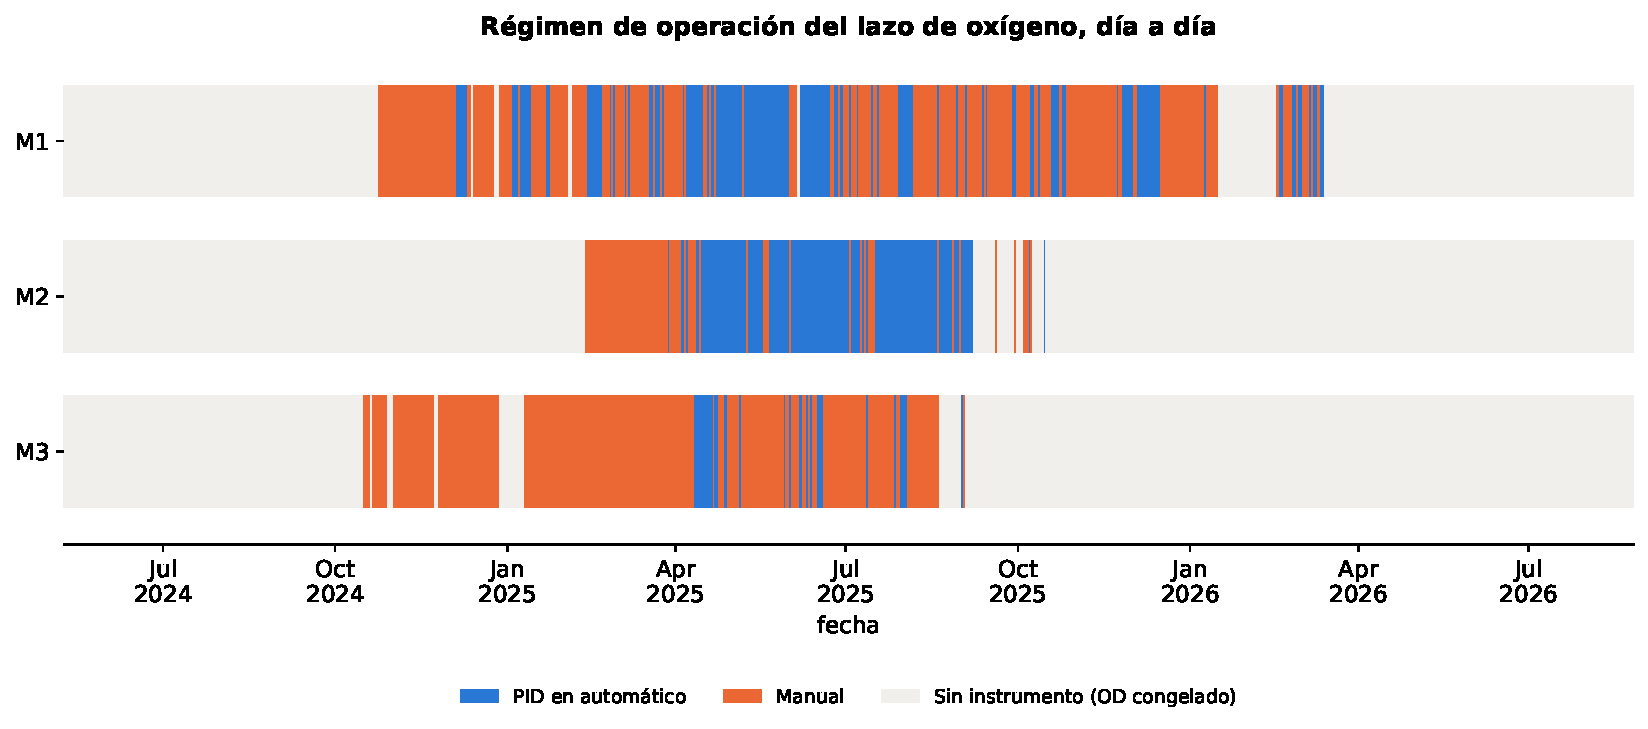
\includegraphics[width=\linewidth]{ident_02_mapa_operacion.pdf}
    \caption[Régimen de operación día a día]{Régimen de operación del lazo de
    oxígeno día a día en los tres módulos. Azul: PID en automático; naranja:
    manual; gris: sensor congelado.}
    \label{fig:ident_mapa}
\end{figure}

% ----------------------------------------------------------------------------
\subsection{Funcionamiento en lazo cerrado con PID}
\label{sec:ident_pid}

La referencia está fija en 2,0~mg/L durante todo el registro, así que no hay
escalones de referencia. Lo equivalente son los arranques del soplador bajo
PID: el lazo parte del OD en el suelo y tiene que llevarlo a la referencia.

La Figura~\ref{fig:ident_pid_arranques} muestra arranques de M2 donde la
variable del proceso (el OD) llega a la referencia sin oscilaciones, con un
sobreimpulso pequeño, de 5,1 y 7,7~\%. El sobreimpulso $M_p$ y el error absoluto medio
$\overline{|e|}$ (Tabla~\ref{tab:metricas}) se calculan desde que arranca el PID, incluyendo la subida
desde el suelo; como el arranque parte de cero, el cambio de consigna es la propia referencia,
$r = 2{,}0$~mg/L, y el sobreimpulso queda en porcentaje de ella. Se usa el error absoluto medio y no el
IAE porque las ventanas no duran lo mismo. El error absoluto medio es de 0,139 y 0,126~mg/L. En
cambio, en la Figura~\ref{fig:ident_pid_oscilatorio}, en
otras fechas, se ve un comportamiento subamortiguado en los dos módulos: un
sobreimpulso de 44~\% en M2 y de 91~\% en M3, y una serie de picos con
envolvente decreciente hasta que llega al estacionario. Desde el arranque, su
error absoluto medio es de 0,179~mg/L en M2 y de 0,297 en M3.

\begin{figure}[H]
    \centering
    \subfloat[Los dos mejores arranques en M2: el OD llega a la referencia sin
    oscilar.]{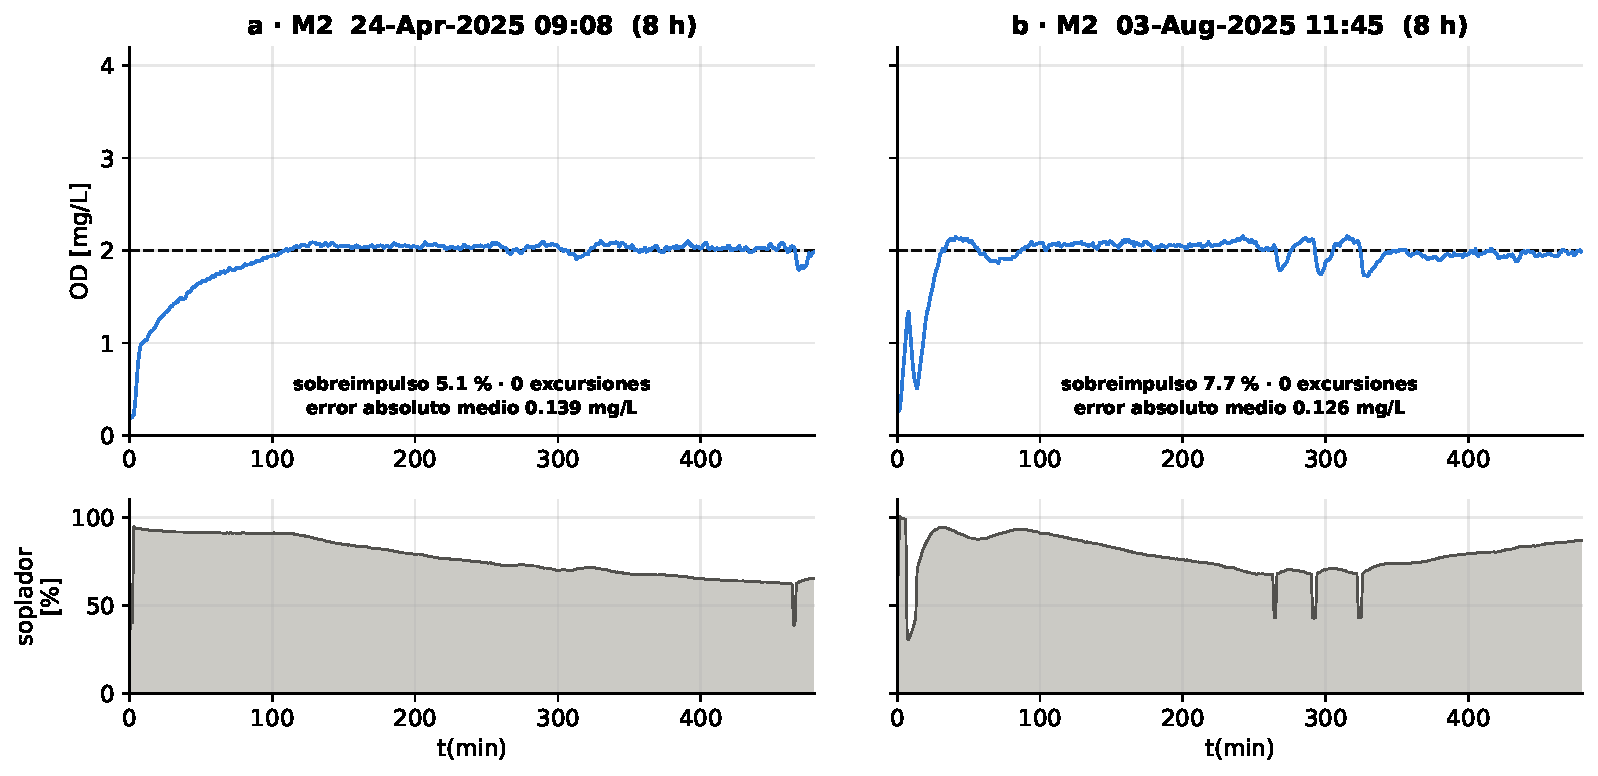
\includegraphics[width=\linewidth]{ident_13_pid_arranques.pdf}%
    \label{fig:ident_pid_arranques}}\\
    \subfloat[Arranques en su versión oscilatoria, en M2 y M3: subamortiguados
    pero convergentes; los círculos marcan los picos sucesivos sobre la
    referencia.]{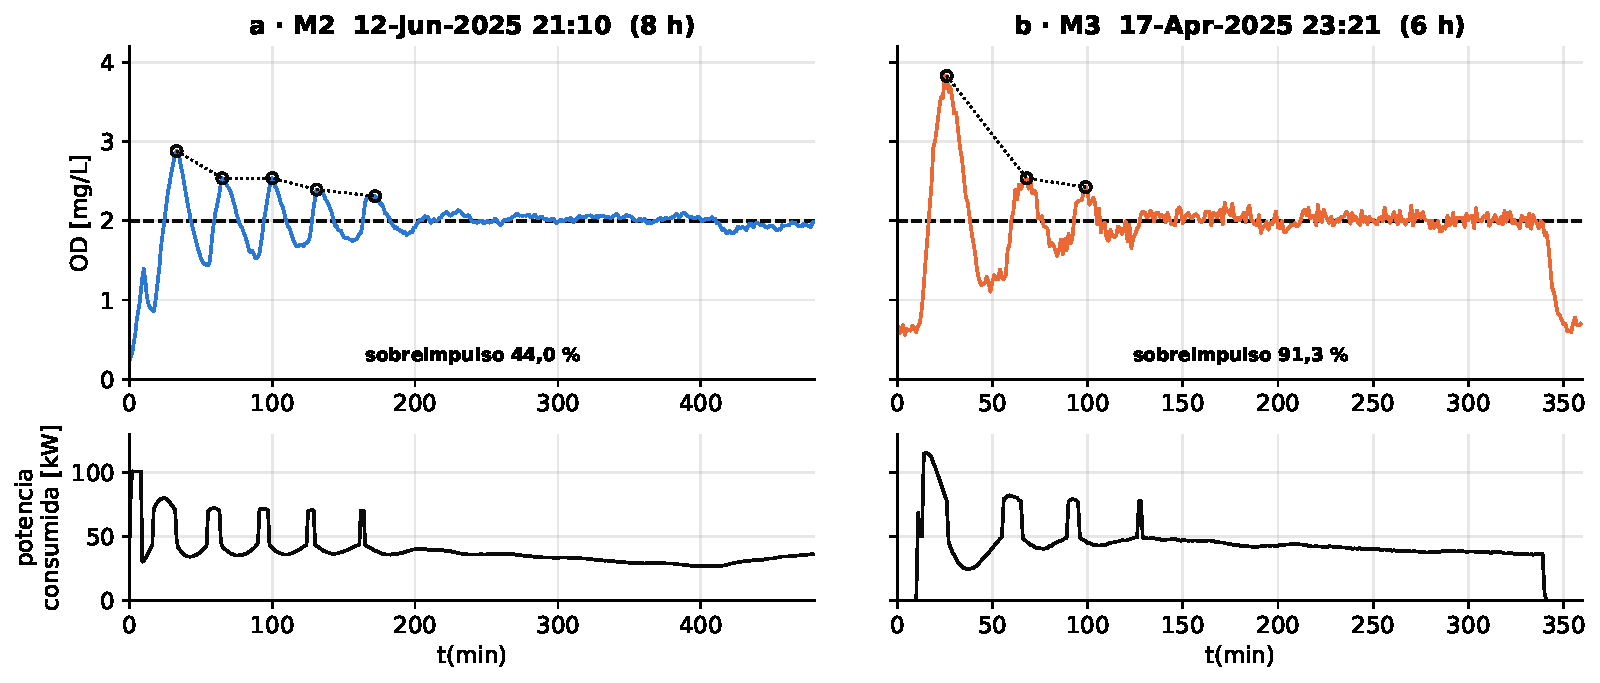
\includegraphics[width=\linewidth]{ident_14_pid_oscilatorio.pdf}%
    \label{fig:ident_pid_oscilatorio}}
    \caption[Arranques del PID actual]{Arranques del PID actual en la planta.
    La línea discontinua es la referencia de 2,0~mg/L; abajo de cada panel, la
    potencia del soplador.}
    \label{fig:ident_pid}
\end{figure}

En resumen, el mismo PID, cuando el sistema tiene condiciones diferentes, a
veces llega a la referencia limpiamente y otras veces oscila. Esto es coherente
con lo que se muestra más adelante en la identificación: la ganancia de la planta cambia de una
ventana a otra (Sección~\ref{sec:ident_arx}), aunque desde el
enfoque del ADRC la ganancia se mantiene constante y lo que cambia es la
perturbación total del sistema. Ahora bien, en algunos casos el OD está en el
suelo y la planta casi no responde; por consiguiente, el PID acumula acción
integral. Cuando el sistema se libera y tiene las condiciones para elevar el
oxígeno, el control puede estar ya saturado por la acumulación de la acción
integral, lo que produce sobreimpulso y algunas oscilaciones, y en los casos en
que no se tenga un sistema de anti-\emph{windup}, el lazo puede volverse
inestable. Por ello, en capítulos posteriores se utilizará para el GPI un
esquema de anti-\emph{windup} que ayude con el manejo de la saturación.



% ----------------------------------------------------------------------------
\subsection{Escalones de soplador en lazo abierto}
\label{sec:ident_escalones}

En los días de operación manual los operarios encienden y apagan el soplador a
mano, con escalones de distinto tamaño y duración. Sin proponérselo, eso es un
ensayo de identificación: hay excitación en la entrada (la potencia) y respuesta
en la salida (el OD), y el lazo no realimenta. En esos escalones el OD tarda más
en subir que en bajar; esa asimetría reaparece en todo el análisis y es algo que
un modelo lineal de primer orden no puede reproducir.


 Ahora bien, si se toman puntos del
histórico u otro escalón, el resultado puede ser un sistema dinámico con
parámetros diferentes. En un proceso tan incierto y con tantas perturbaciones,
la ganancia varía, y a su vez depende de las perturbaciones endógenas y
exógenas del sistema. Lo mismo pasa al comparar los módulos: aunque el proceso
es el mismo en los tres y están dimensionados de igual forma, muestran
dinámicas diferentes. Si se modelan la ganancia y la $\tau$ de cada uno, puede
que no coincidan, y que uno tenga una ganancia bastante mayor que otro. Eso no
significa que los modelos sean distintos, sino que las perturbaciones externas
y las no linealidades afectan al sistema, y que cada uno está trabajando en una
región distinta de su dinámica.

Un ejemplo está en el propio M2. El 16-abr-2025 el soplador va de 0 a unos
93~\% partiendo del suelo, en potencia expresada en porcentaje, que como se
explicó arriba se toma igual a la consigna, y el OD asienta en 3,06~mg/L
(Figura~\ref{fig:ident_escalon_3mgL}). El ajuste da $\tau = 18{,}8$~min y
$K = 0{,}031$~mg/(L$\cdot$\%). El 26-feb-2025, con prácticamente la misma
potencia (95~\%) y partiendo del mismo suelo, el OD asienta en 1,93~mg/L, con
$\tau = 21{,}4$~min y $K = 0{,}018$~mg/(L$\cdot$\%)
(Figura~\ref{fig:ident_escalon_3mgL}b). Con la misma entrada, el estacionario
es 1,58 veces mayor y la ganancia 1,72 veces mayor. Las dos curvas arrancan
juntas y tienen casi la misma constante de tiempo; lo que cambia es el nivel al
que llegan. Por ende, más que dos plantas distintas, es la misma planta cuya
ganancia cambia con las perturbaciones.

\begin{figure}[H]
    \centering
    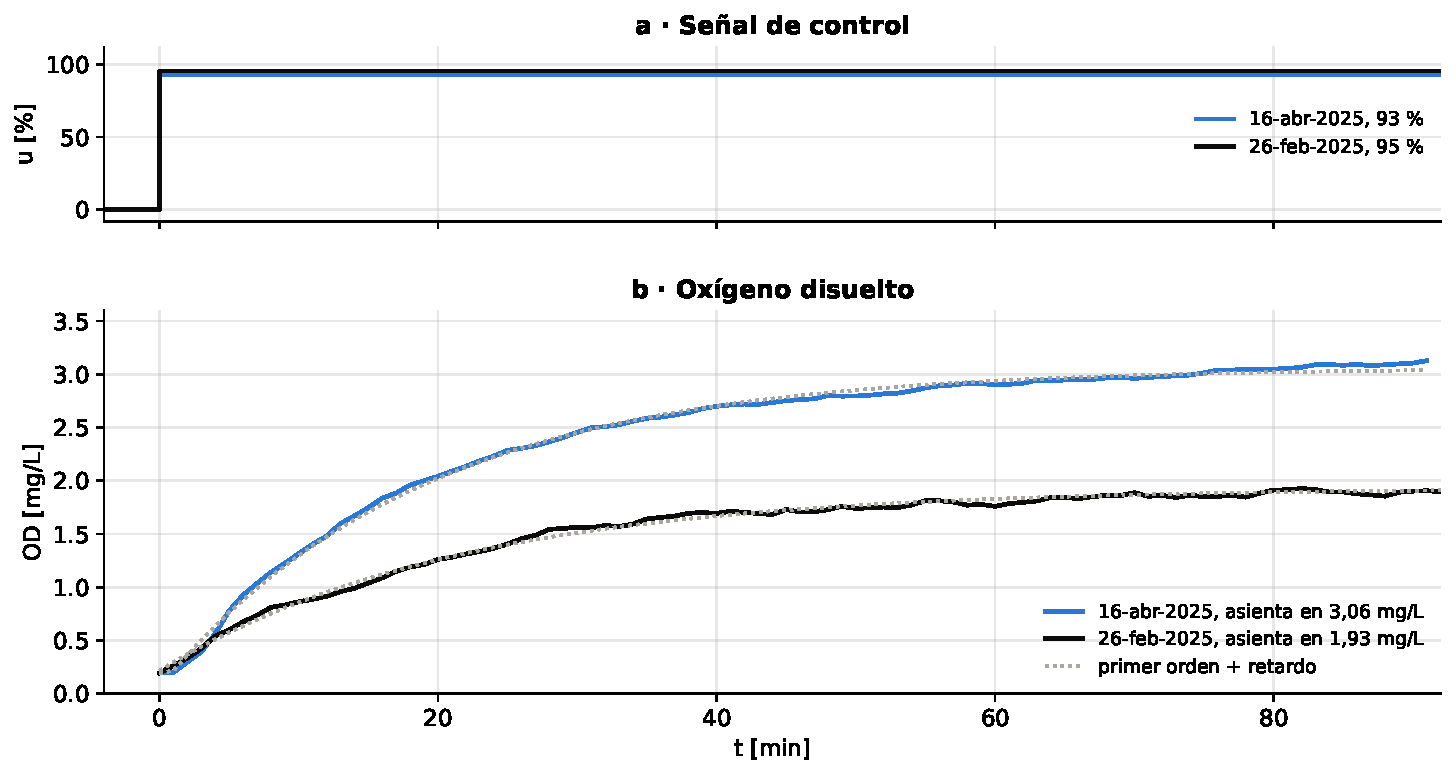
\includegraphics[width=0.85\linewidth]{ident_16_escalon_3mgL.pdf}
    \caption[El mismo escalón de M2 en dos días]{El mismo escalón de M2 en dos días, el 16-abr-2025 y
    el 26-feb-2025: (a) señal de control en porcentaje y (b) OD, que asienta en 3,06 y 1,93~mg/L. La
    línea punteada es el ajuste de primer orden con retardo.}
    \label{fig:ident_escalon_3mgL}
\end{figure}

\paragraph{Un escalón alrededor de la referencia.} Casi todos los escalones
anteriores van de soplador apagado a plena carga, y el OD recorre de casi 0 a
más de 4~mg/L. Por lo que, si se va a trabajar en un punto de operación y regular alrededor de él, se
aconseja realizar la identificación de la ganancia cerca a ese punto: por ejemplo, llegar al estacionario
cerca al punto de operación, hacer un cambio en la señal de control en lazo abierto y medir cuánto varía
la salida. Cerca a un punto de operación se trabaja en una zona que aproximadamente se comporta de forma
lineal, por lo que el sistema puede comportarse mucho mejor en la regulación cuando ya esté en ese punto;
es decir, el modelo lineal es válido solo en la vecindad del punto de operación.
En M3 hay una identificación en el punto de operación, realizada el 13-jun-2025
(Figura~\ref{fig:ident_escalon_ref}). Con 40~kW el OD se asienta en
1,08~mg/L; a las 04:16 la potencia sube a 60~kW ($\Delta u = 18{,}1$~\% de
plena carga) y el OD llega a 2,50~mg/L.
\begin{equation*}
K = \frac{\Delta y}{\Delta u} = \frac{2{,}50 - 1{,}08}{18{,}1}
  = 0{,}079~\mathrm{mg/(L\cdot\%)},
\end{equation*}

\begin{figure}[H]
    \centering
    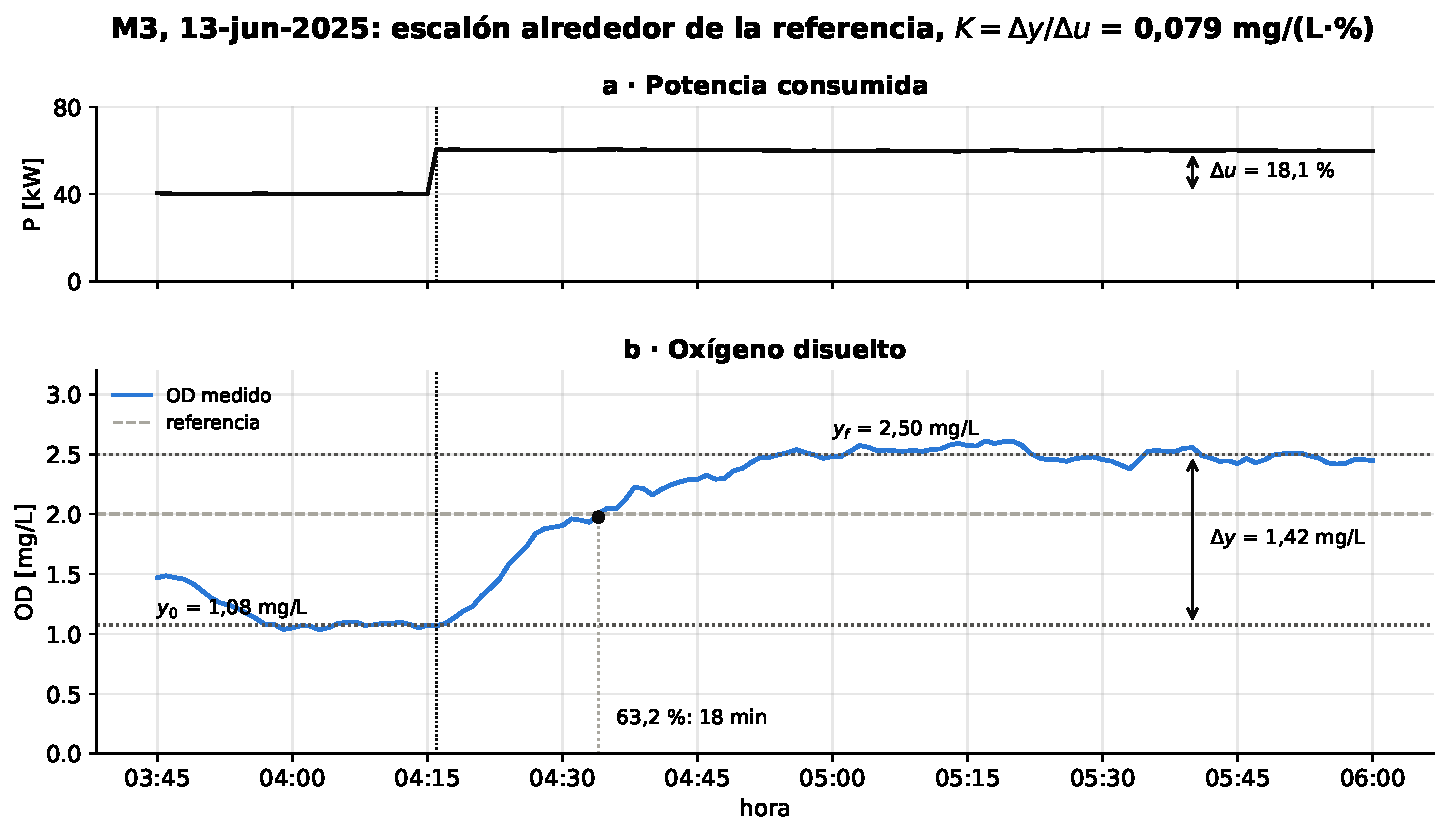
\includegraphics[width=0.85\linewidth]{ident_21_escalon_referencia.pdf}
    \caption[Escalón alrededor de la referencia]{Escalón de M3 del 13-jun-2025
    alrededor de la referencia: (a) la potencia pasa de 40 a 60~kW a las 04:16 y
    (b) el OD va de 1,08 a 2,50~mg/L, con $K = \Delta y/\Delta u = 0{,}079$~mg/(L$\cdot$\%).}
    \label{fig:ident_escalon_ref}
\end{figure}

% ----------------------------------------------------------------------------
\subsection{Segundo soplador}
\label{sec:ident_segundo_soplador}

La planta se operaba con una sola señal de control de 0 a $100~\%$ repartida entre los dos
sopladores: el primer $50~\%$ de la señal lleva un soplador hasta su máximo y el otro $50~\%$ es para
el segundo. En la Figura~\ref{fig:ident_segundo_soplador}, con un soplador el OD se queda casi quieto,
y al entrar el segundo sube rápido; cuando se apaga, vuelve a bajar. Por eso se decidió conectar los
dos sopladores a la misma señal de control de 0 a $100~\%$, sin fraccionarla. Aun así, el ADRC debería
poder asimilar la entrada del segundo soplador: mientras el sistema no llegue a la referencia actúa el
anti-\emph{windup}, y cuando entra el segundo soplador, el exceso de potencia que aporta se toma como una
perturbación y el sistema llega a la referencia.

\begin{figure}[H]
    \centering
    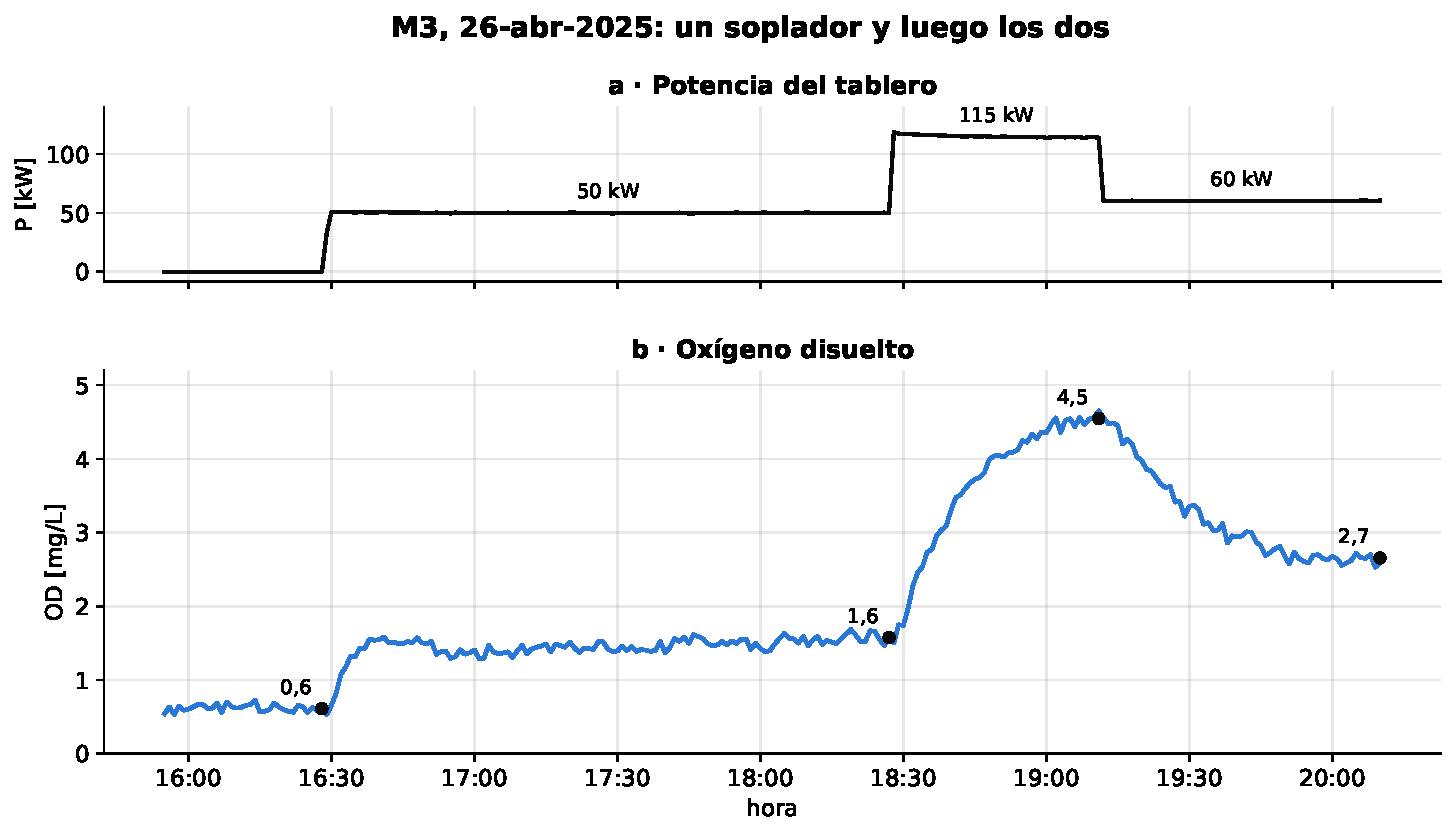
\includegraphics[width=0.85\linewidth]{ident_22_segundo_soplador.pdf}
    \caption[Entrada del segundo soplador en M3]{M3 el 26-abr-2025: (a) potencia del tablero y (b) OD,
    con el valor que alcanza al final de cada cambio de potencia: apagado, un soplador a 50~kW, los dos a
    115~kW y de nuevo uno a 60~kW.}
    \label{fig:ident_segundo_soplador}
\end{figure}

% ----------------------------------------------------------------------------
\subsection{Retardo}
\label{sec:ident_retardo}

El SCADA, a 1~min, no puede resolver un retardo de menos de un minuto. El único
escalón que sí lo resuelve es el registrado por el PLC a 50~ms
(Figura~\ref{fig:ident_retardo}). La imagen muestra un retardo aproximado de
$\theta = 50$~s, y el OD sale de su ruido a los $\approx$ 58~s. A simple vista, el OD empieza a subir hacia los 50~s. Por
ende, para el diseño se considera un retardo entre 0 y 60~s, con ideal de 50~s, que abarca el espectro completo de $\theta$, y en
simulación se valida el controlador con estas variaciones del retardo.

\begin{figure}[H]
    \centering
    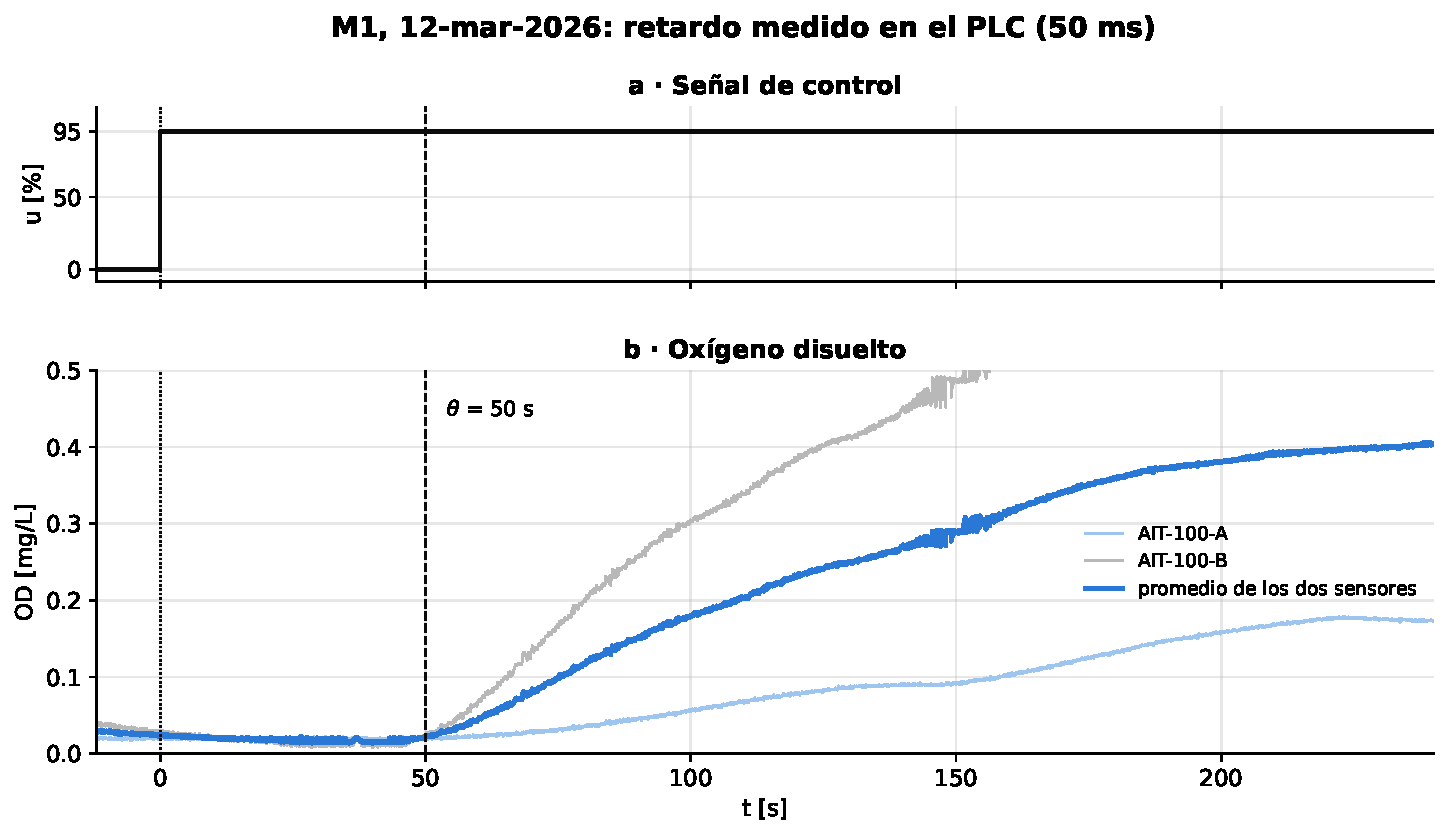
\includegraphics[width=0.85\linewidth]{ident_10_retardo_M1.pdf}
    \caption[Retardo medido en M1]{Primeros 4~min del escalón del
    12-mar-2026 en M1, registrado por el PLC ctrlX a 50~ms: (a) señal de control
    $u$ y (b) OD. La línea discontinua marca el retardo observado del sistema (50~s).}
    \label{fig:ident_retardo}
\end{figure}

% ----------------------------------------------------------------------------
\subsection{Rango de variación de $\tau$ y $K$}
\label{sec:ident_arx}

Sobre los días de lazo abierto se ajusta, en ventanas de 3~h, un modelo de
primer orden en tiempo discreto. Se utiliza una identificación ARX
(autorregresiva con entrada exógena), la más simple posible: un ARX(1,1) de
primer orden con término constante, estimado por mínimos cuadrados:
\begin{equation}
y[k+1] = \varphi\, y[k] + \gamma\, u[k] + \delta ,
\end{equation}
con $y$ el OD (oxígeno disuelto) y $u$ la señal de control en porcentaje,
obtenida a partir de los datos de potencia medidos. De sus coeficientes salen
$\tau = -T_s/\ln\varphi$, $K = \gamma/(1-\varphi)$ y $\bo = K/\tau$.

Ahora bien, la consigna de 0 a 100~\% que el PLC envía a los variadores no
quedó registrada en el histórico del SCADA; lo que sí se registra es la
potencia eléctrica del tablero de aireación. Por eso, en este trabajo se toma
la potencia expresada en porcentaje de plena carga,
$u = 100\,P/P_{\max}$ (con $P_{\max} = 106{,}3$~kW en M2 y $110{,}1$~kW en
M3), como si fuera la misma señal de control. Entre las dos está la cadena de
actuación (variador, motor y soplador), que no es exactamente lineal; esa
discrepancia no se modela por separado, sino que queda incluida en la
perturbación total $\bar{\xi}$, igual que el error que se cometa al elegir $\bo$
(Sección~\ref{sec:car_modelo}). Es decir, el observador del ADRC la estima y la
compensa junto con el resto de lo que el modelo no representa. 
La Figura~\ref{fig:ident_pulso} muestra una ventana con su respectiva
identificación ante un escalón del soplador. Un solo par ($\tau = 15$~min,
$K = 0{,}036$) reproduce el arranque y el estacionario con un $R^2$ de
simulación de 0,95. En la figura también se observa la asimetría de la planta:
el OD real sube al 63~\% en 24~min y cae en 8~min, mientras que el modelo tarda
lo mismo en ambos sentidos; es decir, el modelo promedia la dinámica de subida
y la de bajada. Esa diferencia es precisamente lo que el observador del ADRC
agrupa en la perturbación total y estima en línea.

\begin{figure}[H]
    \centering
    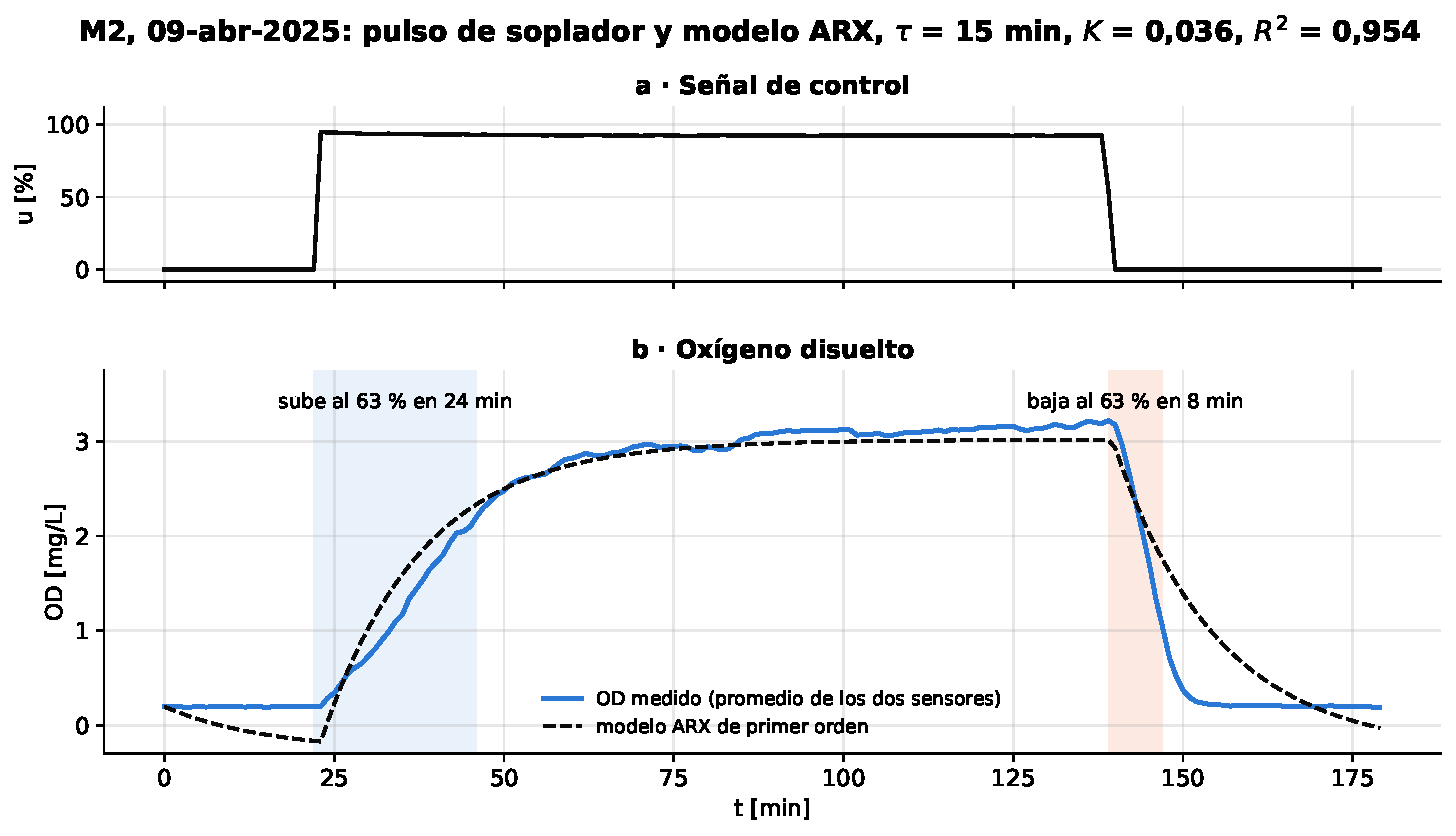
\includegraphics[width=0.85\linewidth]{ident_03_pulso_arx.pdf}
    \caption[Identificación ARX sobre un pulso]{Ajuste ARX sobre una ventana de
    3~h de M2 en lazo abierto y validación por simulación libre. Las franjas
    marcan el tiempo al 63~\% medido en el dato al subir y al bajar.}
    \label{fig:ident_pulso}
\end{figure}

Ahora bien, en la literatura, cuando se diseña un controlador lineal para un
sistema no lineal, lo usual es linealizar alrededor de un punto de operación:
se aplican escalones pequeños cerca de ese punto, se identifica la ganancia
local $\Delta y/\Delta u$ y se diseña el controlador para que regule dentro de
esa región. En este trabajo el diseño también se hizo en un punto de operación,
el de 2~mg/L (Sección~\ref{sec:ident_planta_diseno}), y para llegar a él se
acondiciona la referencia (Sección~\ref{sec:impl_referencia}), de modo que el
sistema llegue suavemente a la consigna, independientemente de la que se elija.
La identificación, en cambio, se hizo con todos los escalones recolectados, en
todo el rango de operación de la planta y del actuador, porque se quería conocer
el rango en el que varían la ganancia y la constante de tiempo del sistema, y
verificar que el ADRC, ante esas diferentes ganancias, funciona dentro de lo
esperado sin cambiar sus parámetros.

Paralelamente, la asimetría de la planta se puede medir sobre todo el registro.
Para eso se toman los 532 escalones de soplador que pasan un filtro estricto
($|\Delta u| \geq 20$~\%, al menos 90~min de duración, $R^2 \geq 0{,}90$,
respuesta asentada y $|\Delta y| \geq 0{,}30$~mg/L) y se ajusta cada uno con un
primer orden con retardo. Cuando se sube la aireación, $\tau$ tiene una mediana
de 43~min en M2 y de 36 en M3; cuando se baja, de 4 y 7~min (sus distribuciones
completas están en la Figura~\ref{fig:ident_pob}). El oxígeno cae en minutos y
sube en media hora. El controlador tiene que tolerar esa asimetría sin conmutar
parámetros, y es una de las cosas que el observador del ADRC absorbe dentro de
la perturbación total.

Ahora bien, con el ARX se buscan modelos lineales aproximados repitiendo el
ajuste en ventanas deslizantes de 3~h con paso de 1~h, y descartando las
ventanas sin excitación, con $R^2 < 0{,}5$ o con $\tau$ fuera de 1--300~min.
Así quedan 1.225 ventanas de lazo abierto en M2 y 1.822 en M3. Sus distribuciones
(Figura~\ref{fig:ident_pob}) son anchas: la
identificación promedia la subida y la bajada, y además la ganancia cambia de una
ventana a otra. Por eso se
reportan medianas: $\tau = 16{,}9$~min y $K = 0{,}0201$ en M2, y
$\tau = 24{,}4$~min y $K = 0{,}0649$ en M3. Como rango se usa el
intercuartílico, es decir, el intervalo donde cae la mitad central de las
ventanas: en M2, $K$ va de 0,008 a 0,034 (unas 4 veces) y $\tau$ de 11 a
26~min. Con esto ya se obtiene el espectro de los parámetros que rigen la
dinámica del sistema.

\subsection{Validación del modelo}
\label{sec:ident_validacion}

Con el ARX se obtuvo un modelo lineal de primer orden en cada ventana. Ahora
bien, falta responder si ese modelo realmente abarca la mayor parte de la
información del fenómeno. Para eso se comparan los parámetros del ARX con los
de los escalones medidos directamente en la planta, primero como poblaciones y
después escalón por escalón.

Los escalones de soplador son la referencia más directa del comportamiento real: en cada uno se
ve cuánto tarda el OD en responder y cuánto llega a cambiar, por separado para
las subidas y para las bajadas. Si el modelo ARX representa bien la planta, sus
parámetros deberían parecerse a los de los escalones.

La Figura~\ref{fig:ident_pob} pone las tres poblaciones juntas: las ventanas
ARX, los escalones que suben y los escalones que bajan. Como hay muchas más
ventanas ARX que escalones, cada histograma se normaliza como densidad: si $N$
es el número de ajustes de una población, $n_j$ el número que cae en el
intervalo $j$ y $\Delta$ el ancho del intervalo, la altura de la barra es:

\begin{equation}
    \hat f_j = \frac{n_j}{N\,\Delta},
    \qquad
    \sum_j \hat f_j\,\Delta = 1 ,
    \label{eq:ident_densidad}
\end{equation}

de modo que el área de cada histograma vale 1 y las poblaciones se pueden
comparar aunque tengan tamaños muy distintos. El eje horizontal está en escala
logarítmica, con intervalos de igual ancho en $\log_{10}$ (y $\Delta$ medido en esa
escala): las tres magnitudes son positivas y se comparan por cocientes, y en
esa escala su forma es casi simétrica.

\begin{figure}[H]
    \centering
    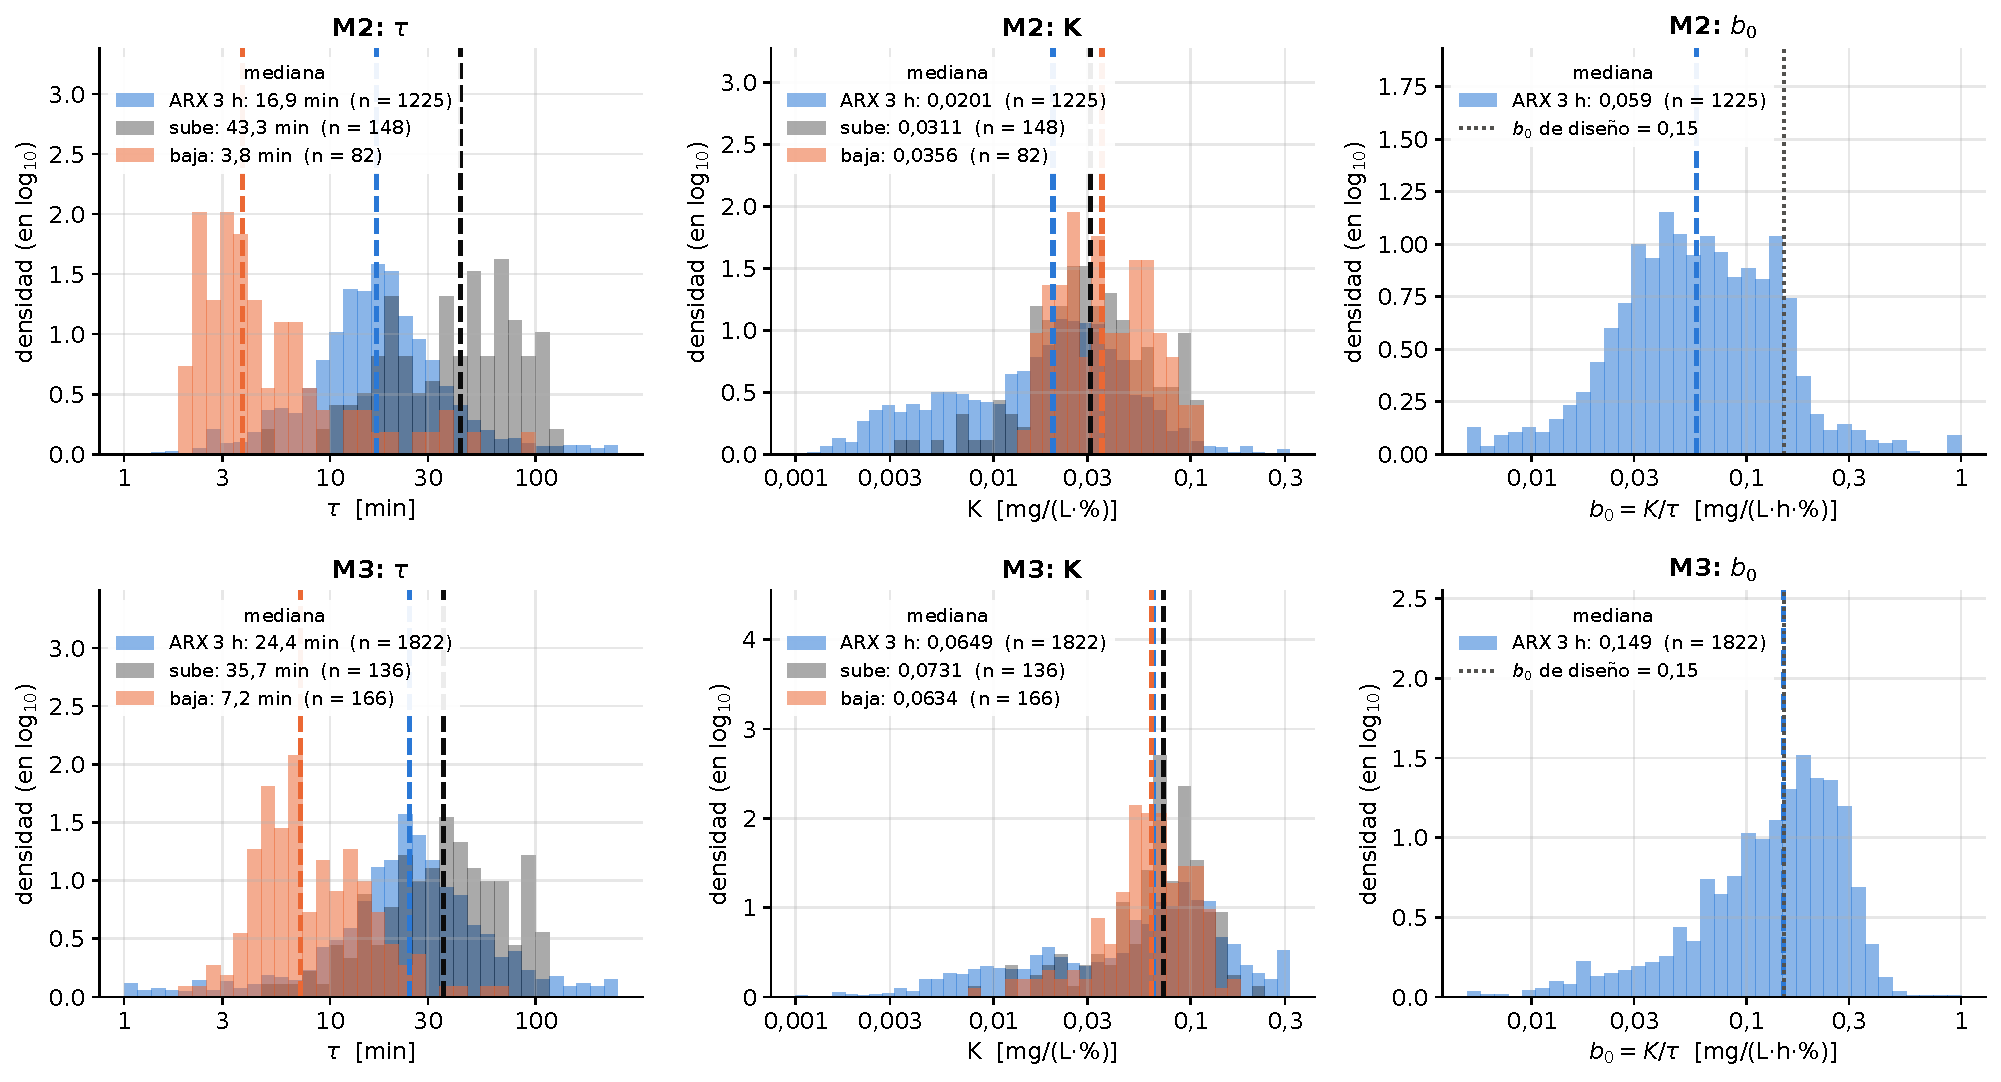
\includegraphics[width=\linewidth]{ident_05_poblaciones_tau_K.pdf}
    \caption[Poblaciones de $\tau$, $K$ y $\bo$ en M2 y M3]{Las tres poblaciones
    de la constante de tiempo (izquierda), de la ganancia estática (centro) y de
    la ganancia de entrada $\bo = K/\tau$ (derecha) en M2 (arriba) y M3 (abajo):
    ventanas ARX de 3~h, escalones que suben y escalones que bajan (en $\bo$,
    solo las ventanas ARX). Histogramas en densidad según
    \eqref{eq:ident_densidad}, con el eje horizontal en escala logarítmica; las
    líneas discontinuas son las medianas, la punteada de la derecha es el $\bo$
    de diseño (0,15) y los valores fuera del eje se acumulan en las barras de los
    extremos.}
    \label{fig:ident_pob}
\end{figure}

En la constante de tiempo (columna izquierda) las tres poblaciones no
coinciden, y eso era de esperarse. Los escalones que suben son lentos y los que
bajan son rápidos: es la asimetría de la planta. El ARX, en cambio, ajusta un
solo $\tau$ en ventanas que contienen subidas y bajadas, por lo que queda en un
valor intermedio entre las dos. Es decir, el modelo lineal trata de abarcar la dinámica
de subida y la de bajada, y no puede reproducir la asimetría.

En la ganancia (columna derecha) el resultado es distinto. Los escalones que
suben y los que bajan dan ganancias parecidas, lo que indica que la asimetría
es solo dinámica: la planta tarda distinto en subir y en bajar, pero llega a un
cambio de OD similar. En M3 el ARX coincide con los escalones; en M2 sale algo
más bajo, porque sus ventanas están, en promedio, en un OD más bajo que el de
los escalones (0,81 frente a 1,41~mg/L).

Por ende, el modelo ARX captura bien el orden de magnitud de la ganancia y una
constante de tiempo promedio, pero no la asimetría. Esa parte que el modelo
lineal no representa es la que el observador del ADRC agrupa dentro de la
perturbación total.

\paragraph{Comparación escalón por escalón.} Los histogramas comparan
poblaciones completas, pero no dicen si el ARX acierta en cada caso. Para
eso, sobre cada escalón limpio se ajustó también el ARX, y se comparó con dos valores que se leen directamente
en el dato, sin ajustar ningún modelo: el tiempo que tarda el OD en recorrer el
63~\% del salto ($t_{63}:\tau$) y la ganancia real, $\Delta y/\Delta u$, medida como
el cambio de OD dividido por el cambio de la señal de control. La
Figura~\ref{fig:ident_validacion} muestra el resultado: cada punto es un
escalón, el eje horizontal es el valor medido y el vertical el del ARX, y la
diagonal punteada indica que los dos coinciden.

\begin{figure}[H]
    \centering
    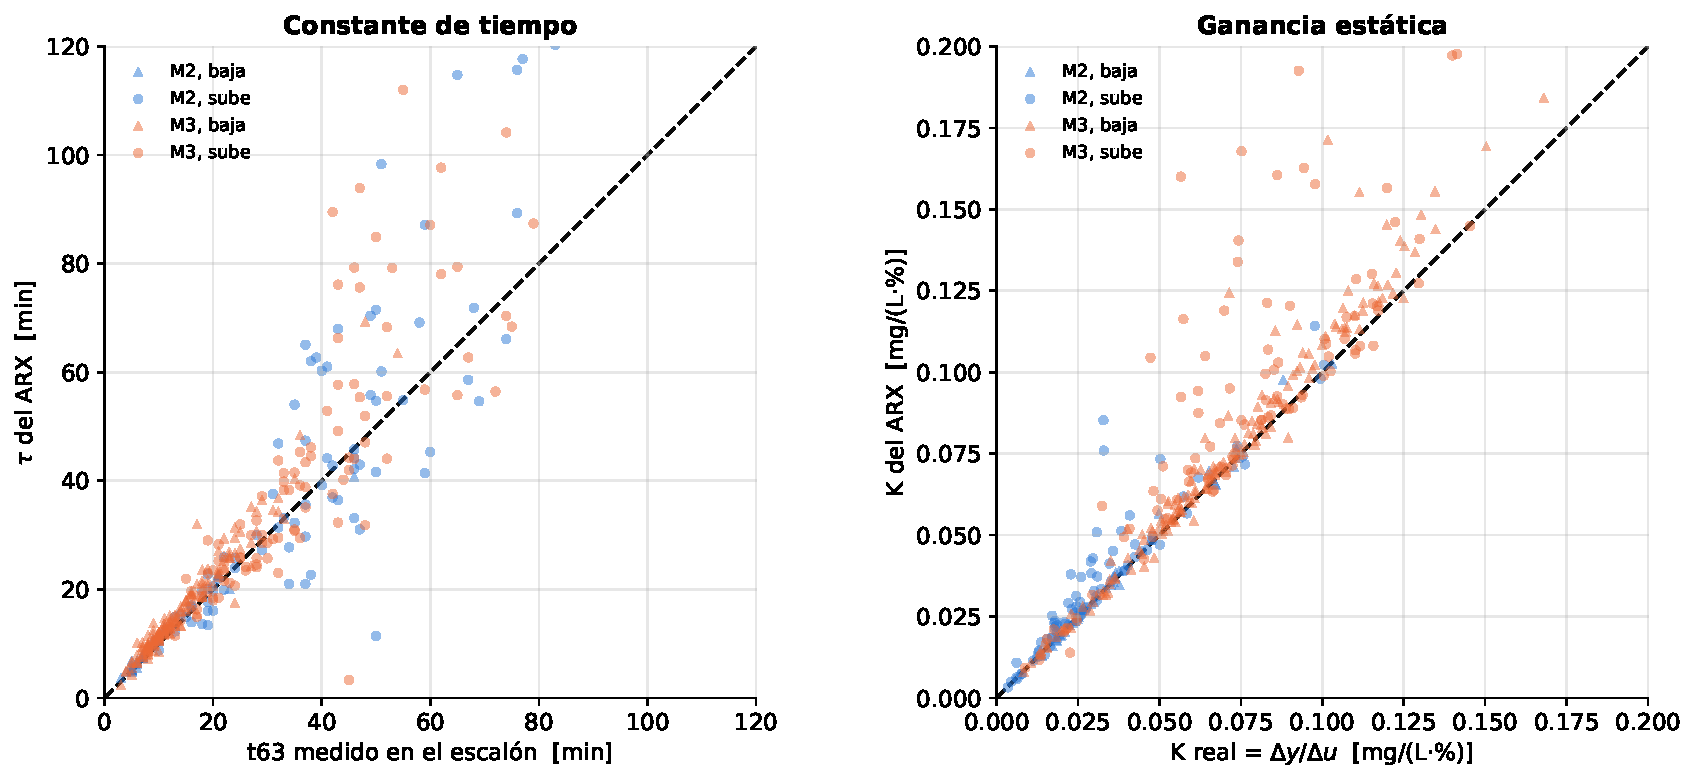
\includegraphics[width=\linewidth]{ident_10_validacion_arx.pdf}
    \caption[Validación del ARX escalón por escalón]{Validación del ARX escalón
    por escalón. Izquierda: constante de tiempo del ARX frente al tiempo al
    63~\% medido en el dato. Derecha: ganancia del ARX frente a la ganancia
    real $\Delta y/\Delta u$. Círculos: escalones que suben; triángulos:
    escalones que bajan. La diagonal es la igualdad.}
    \label{fig:ident_validacion}
\end{figure}

En la ganancia los puntos caen sobre la diagonal en todo el rango, tanto en M2
como en M3 y tanto al subir como al bajar. En la constante de tiempo también siguen la
diagonal; las bajadas, que son rápidas, quedan muy pegadas a ella, y las
subidas lentas se dispersan más, porque al arrancar desde un OD muy bajo la
respuesta no es una exponencial limpia. Por ende, cuando el ARX mira un solo
escalón reproduce lo que se mide en la planta, y esto valida que el espectro de
ganancias que entrega la identificación (Sección~\ref{sec:ident_arx}) es
el de la planta.



% ----------------------------------------------------------------------------
\subsection{Perfil diario de los caudales}
\label{sec:ident_caudales}

Los caudales de M2 se toman del historiador del SCADA, que registra cada hora,
en L/s, el caudal de entrada a la salida del desarenador (FIT-101) y el de
recirculación de lodos (FIT-102). Cada registro es una muestra instantánea del
caudal en ese momento. La
Figura~\ref{fig:ident_caudales_perfil}a muestra un día completo de los dos
caudales, tal como los guarda el SCADA. La recirculación, en cambio, solo se enciende durante periodos cortos. Aun así, el controlador debe poder
rechazar esos cambios y, si llegara a saturarse mientras la bomba está
encendida, mantener la saturación controlada hasta que se apague.


Ahora bien, el caudal cambia de un día para otro y varía aleatoriamente. No es predecible; lo que se puede
medir es el rango en el que los operarios lo tratan de mantener o el valor de referencia que se debe tener.
En la Figura~\ref{fig:ident_caudales_perfil}b, siete días seguidos se
superponen al ciclo diario (la media de los datos medidos en cada hora durante los días de referencia) y ninguno lo sigue; la banda que contiene la mitad central
de los registros de cada hora mide unos 18~L/s de ancho, el doble de lo que varía
el ciclo. Lo que cada registro se aparta del ciclo tiene una desviación estándar
robusta de 13,6~L/s. Es decir, el caudal de entrada es sobre todo aleatorio, con un ciclo
diario débil que está alrededor de un valor de DC de aproximadamente 34~L/s. Por ende, la perturbación, que depende de los caudales de entrada
según la ecuación~\eqref{ecu:disturbance} que se modela en la sección
siguiente tiene la misma estructura: un nivel $\bar{\xi}_0$, un ciclo diario y una parte
aleatoria de mayor magnitud.

\begin{figure}[H]
    \centering
    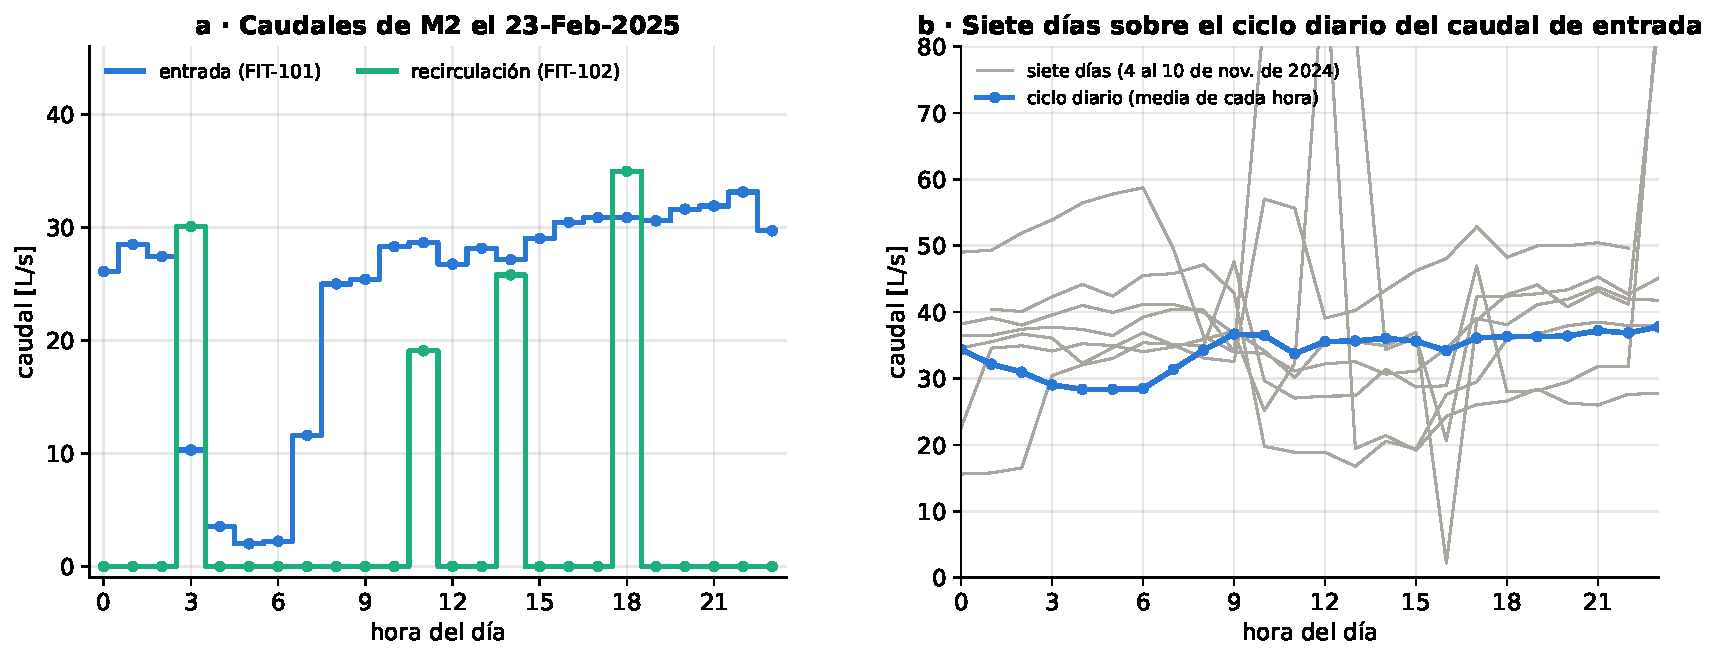
\includegraphics[width=\linewidth]{ident_11_caudales_perfil.pdf}
    \caption[Caudales de M2]{Caudales de M2: (a) entrada (FIT-101) y
    recirculación (FIT-102) el 23 de febrero de 2025, con un registro por hora
    del SCADA; (b) caudal de entrada del 4 al 10 de noviembre de 2024 (en gris)
    sobre su ciclo diario (media de cada hora); la banda contiene el 50~\%
    central de los registros de cada hora.}
    \label{fig:ident_caudales_perfil}
\end{figure}



% ----------------------------------------------------------------------------
\subsection{Reconstrucción de la perturbación total (sintética)}
\label{sec:ident_perturbacion}

Si bien para sintonizar los controladores no es necesario conocer la
perturbación completa, sí se puede usar para simularlos y para sintonizar el
observador. Por ende, la perturbación total $\bar{\xi}$ de $\dot y = \bar{\xi} + \bo u$ se
define como señal en el tiempo. Como no se puede medir, se reconstruye una señal
que no es la real, pero que conserva lo principal de ella (su nivel DC, su
variación y algo del contenido en frecuencia) y que sale de datos reales de la
planta: los coeficientes del ARX de cada ventana de lazo abierto de M2
(Sección~\ref{sec:ident_arx}). De $\varphi$ y $\gamma$ salen $\tau$ y $\bo$; el
tercer coeficiente, el término constante $\delta$, es lo que mueve el OD sin
depender de $u$. Llevado a tiempo continuo, el modelo de cada ventana es
\begin{equation}
\dot y = -\frac{y}{\tau} + \bo\,u + d,
\qquad
d = \frac{\delta}{\tau\,(1-\varphi)},
\label{eq:ident_arx_continuo}
\end{equation}
donde $d$ se obtiene al exigir que el ARX y el modelo continuo lleguen al mismo
estacionario. Todo lo que no multiplica a $u$ es la perturbación,
$\bar{\xi} = d - y/\tau$, que depende del OD de cada ventana; para que las ventanas
sean comparables, se evalúa en la referencia:
\begin{equation}
\bar{\xi}_2 = d - \frac{2{,}0}{\tau} .
\label{eq:ident_xi2}
\end{equation}
Es la velocidad a la que cambiaría el OD en 2,0~mg/L con el soplador apagado, y
es negativa porque la biomasa consume oxígeno. Las ventanas se toman cada hora
en los días manuales y, tras los filtros de la Sección~\ref{sec:ident_arx},
quedan 1.225 valores de $\bar{\xi}_2$, cada uno fechado en el centro de su ventana.
De ellos se descartan 12 atípicos, los que se apartan más de 10 desviaciones
robustas de la mediana (siete son del 4 al 8 de octubre de 2025, entre $-60$ y
$-162$~mg/(L$\cdot$h)), y quedan 1.213.

Con esos valores, la señal se arma con tres piezas:
\begin{equation}
\bar{\xi}(t) = \bar{\xi}_0 + c(t) + \eta(t),
\label{eq:ident_generador}
\end{equation}
\begin{itemize}
  \item \textbf{Nivel DC}, $\bar{\xi}_0 = -8{,}49$~mg/(L$\cdot$h): la mediana de todas
  las $\bar{\xi}_2$.
  \item \textbf{Ciclo diario}, $c(t)$: la mediana de las $\bar{\xi}_2$ de cada hora del
  día, centrada en cero, unida con rectas entre horas y repetida cada 24~h. Varía 3,46~mg/(L$\cdot$h) pico a
  pico (Figura~\ref{fig:ident_perturbacion}a).
  \item \textbf{Parte aleatoria}, $\eta(t)$: una señal que varía lentamente,
  generada cada minuto como un proceso de Ornstein--Uhlenbeck, con su discretización
  exacta \cite{gillespie1996} (Figura~\ref{fig:ident_perturbacion}b). Sus dos parámetros,
  la desviación $\sigma_\eta$ y la constante de tiempo $\tau_\eta$
  (Tabla~\ref{tab:ident_resumen}), se miden en el residuo de cada ventana,
  $r = \bar{\xi}_2 - \bar{\xi}_0 - c$: $\sigma_\eta$ con el rango intercuartílico, para que
  las colas largas no la inflen, y $\tau_\eta$ con la correlación entre residuos
  separados 1~h.
\end{itemize}
Se arranca con $\eta[0] = 0$ y, para las simulaciones, se generan 14 días, sin
filtro. La
Figura~\ref{fig:ident_perturbacion} muestra los tres primeros, pieza por pieza,
y su panel d, el tipo de cambio que el controlador debe rechazar: en media hora,
$\bar{\xi}$ sube 13,7~mg/(L$\cdot$h), que con $\bo = 0{,}15$ son unos 91 puntos de
soplador. El ruido de la sonda no se suma a $\bar{\xi}$, sino a la salida simulada
(Sección~\ref{sec:ident_ruido}).

\begin{figure}[H]
    \centering
    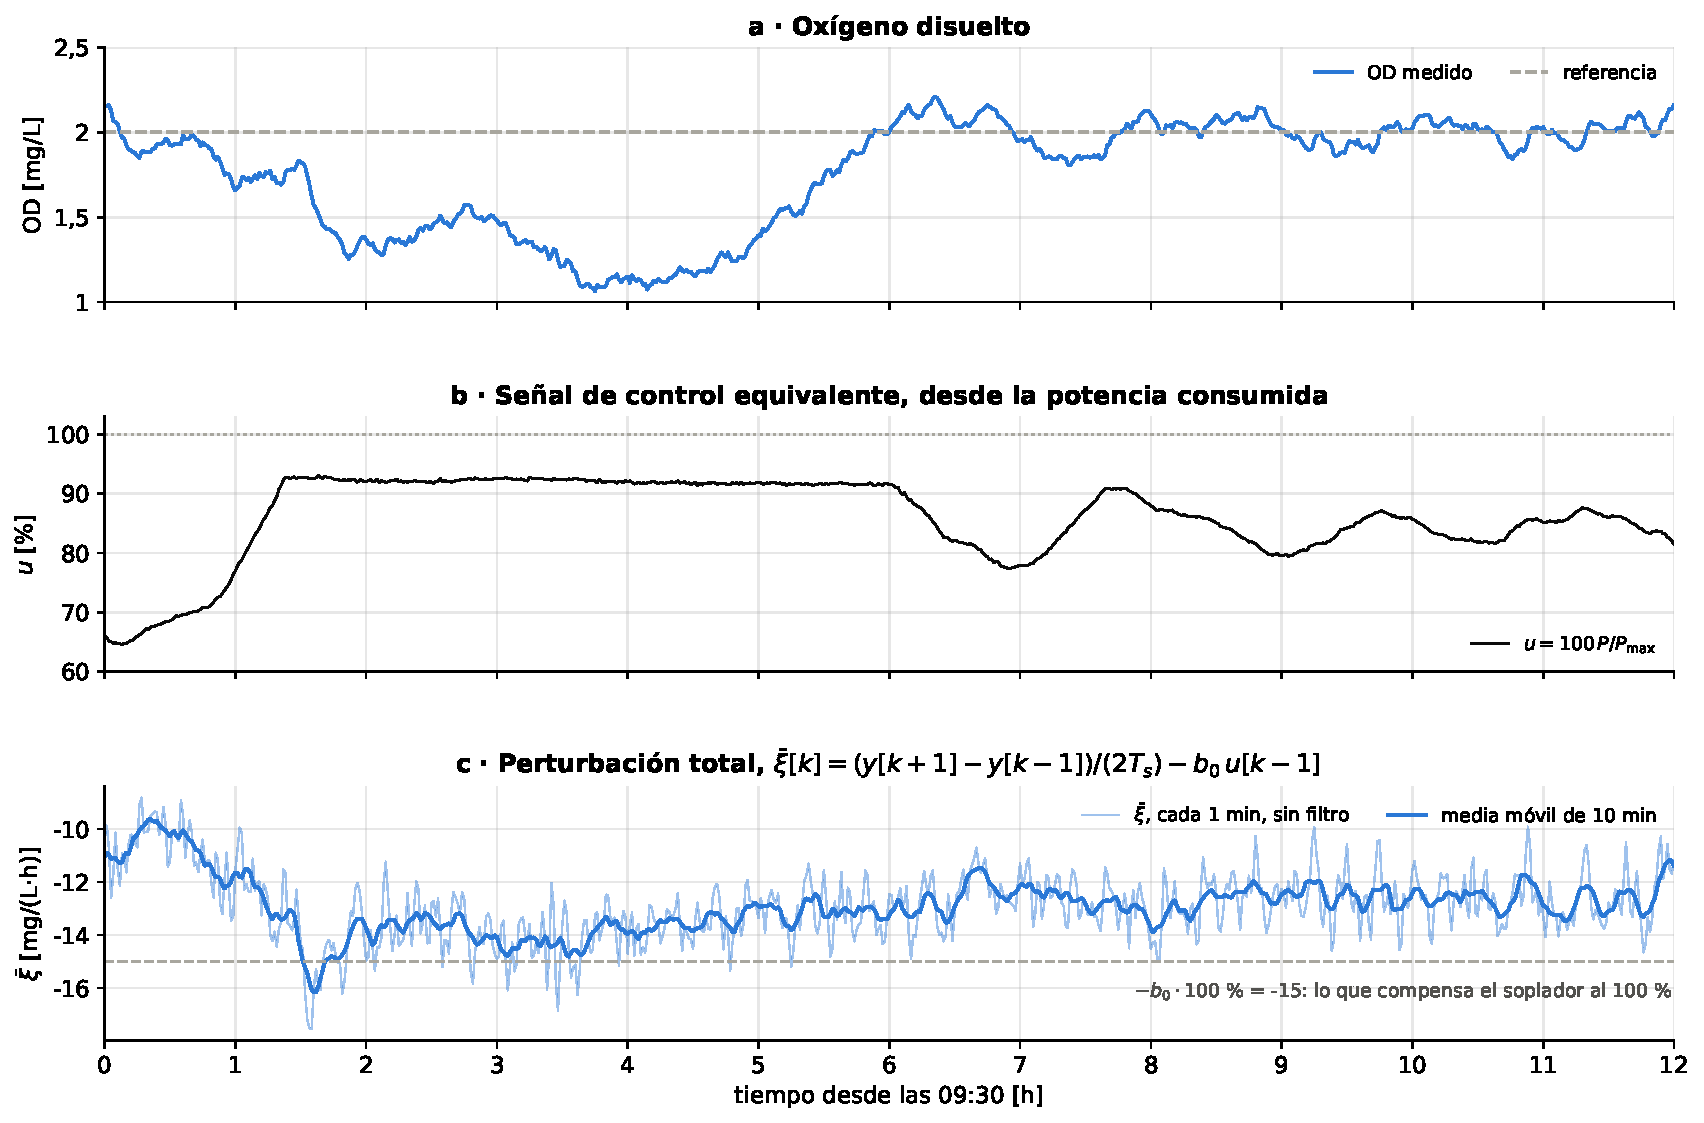
\includegraphics[width=\linewidth]{ident_17_perturbacion.pdf}
    \caption[La perturbación total]{Perturbación total de M2, tres días
    generados a 1~min: (a) nivel y ciclo diario, $\bar{\xi}_0 + c(t)$, con la mediana
    medida de cada hora; (b) parte aleatoria $\eta(t)$; (c) su suma, $\bar{\xi}(t)$; (d)
    las 4~h sombreadas en (c), minuto a minuto y sin filtro. En (b) y (c) se dibuja una media
    móvil de 10~min solo para la visualización; (a), (b) y (c) tienen la misma
    escala vertical.}
    \label{fig:ident_perturbacion}
\end{figure}



% ----------------------------------------------------------------------------
\subsection{Espectro de la perturbación total}
\label{sec:ident_espectro}
El observador del ADRC tiene que seguir a $\bar{\xi}$, así que su ancho de banda $\wo$
debe quedar por encima de las frecuencias donde $\bar{\xi}$ tiene su energía. Para
verlo se calculó el espectro de $\bar{\xi}$ sin filtro con el método de Welch (que tiene ventajas frente a una sola FFT y está disponible en las librerías de MATLAB y Python): la señal
se parte en segmentos de $N = 4096$~min, solapados a la mitad, cada uno se
multiplica por una ventana de Hann (para reducir la fuga espectral), se le aplica
la FFT y se promedian los segmentos. La frecuencia se pasa a rad/h, las unidades
de $\wo$ (Figura~\ref{fig:ident_espectro_f}a), y la fracción de la energía
acumulada hasta la frecuencia $\omega_k$ es
\begin{equation}
E(\omega_k) = 100~\% \cdot \frac{\sum_{i=0}^{k} P[i]}{\sum_{i=0}^{N/2} P[i]},
\label{eq:ident_energia}
\end{equation}
donde $P[i]$ es la densidad espectral en cada frecuencia.
Se usa la $\bar{\xi}$ sintética de M2 (28 días a 1~min, Figura~\ref{fig:ident_espectro_f}),
y la Tabla~\ref{tab:ident_espectro_f} da la frecuencia donde $E$ cruza el 50, 90,
95 y 99~\%.

\begin{figure}[H]
    \centering
    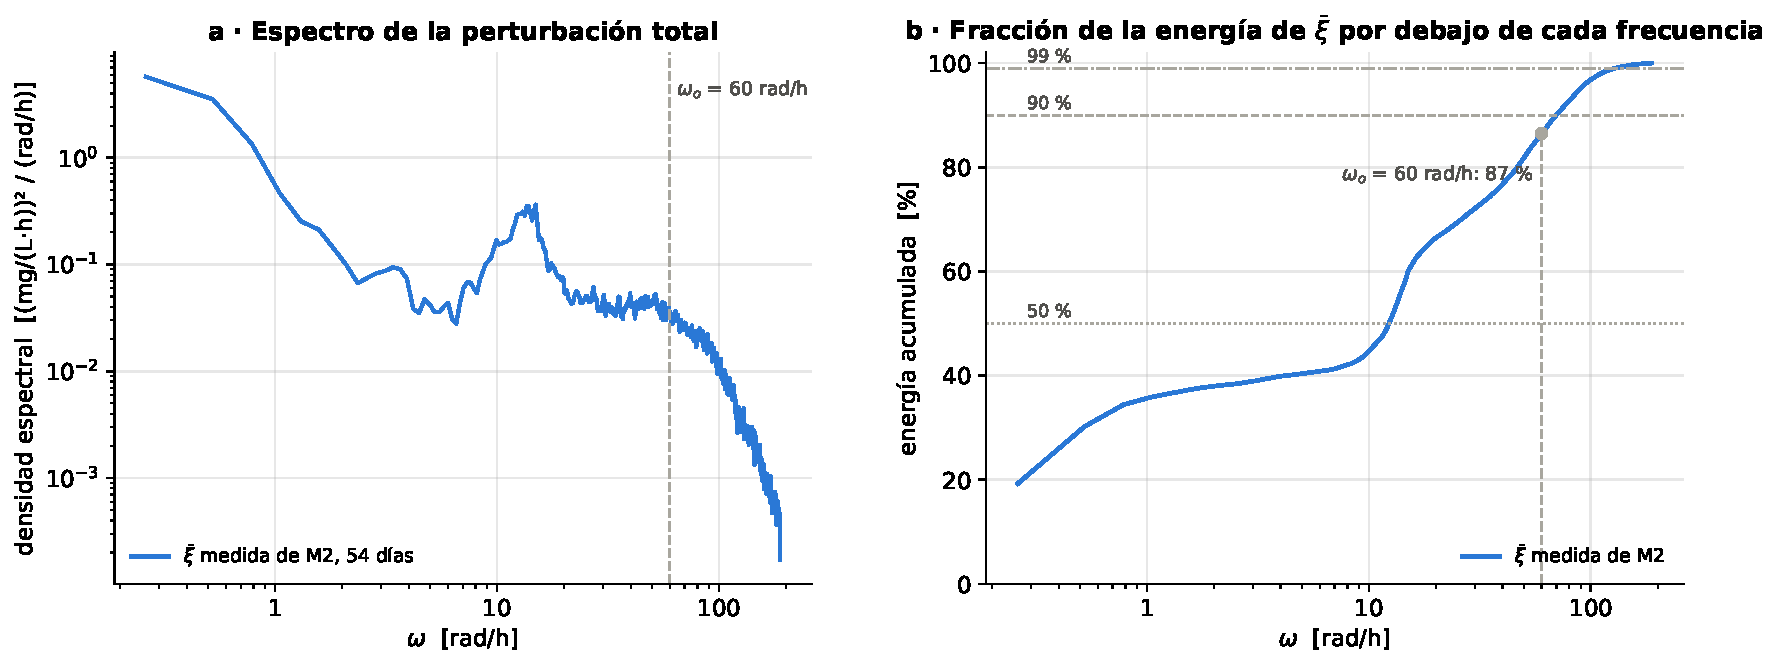
\includegraphics[width=\linewidth]{ident_19_espectro_f.pdf}
    \caption[Espectro de la perturbación total]{Espectro de la perturbación
    total de M2: (a) densidad espectral de la $\bar{\xi}$ sintética; (b)
    fracción de la energía de $\bar{\xi}$ que queda por debajo de cada frecuencia.}
    \label{fig:ident_espectro_f}
\end{figure}

\begin{table}[H]
\centering
\caption{Frecuencia por debajo de la cual queda cada fracción de la energía de
la perturbación total de M2, en rad/h.}
\label{tab:ident_espectro_f}
\small
\begin{tabular}{lcccc}
\toprule
\textbf{Señal} & \textbf{50~\% [rad/h]} & \textbf{90~\% [rad/h]} & \textbf{95~\% [rad/h]} & \textbf{99~\% [rad/h]} \\
\midrule
$\bar{\xi}(t)$ sintética & 1,0 & 6,0 & 12 & 56 \\
\bottomrule
\end{tabular}
\end{table}

La mitad de la energía de la perturbación está por debajo de 1,0~rad/h y el
95~\% por debajo de 12~rad/h. Por ende, para que el observador siga al menos el
95~\% de la energía de $\bar{\xi}$, su ancho de banda debe estar por encima de unos
12~rad/h, y para seguir el 99~\%, por encima de unos 56~rad/h. El límite superior
de $\wo$ no lo pone la perturbación, sino el ruido de la medida y el retardo del
lazo, y se trata en el diseño del observador.

% ----------------------------------------------------------------------------
\subsection{Ruido del sensor}
\label{sec:ident_ruido}

El ruido del sensor de OD se midió con una sola medida: la traza del PLC
a 50~ms del ensayo del 12 de marzo de 2026 en M1. Se usan los últimos
10~min del escalón, con la consigna del soplador fija en 95~\% y el OD cerca de
su estacionario (Figura~\ref{fig:ident_ruido}), se usa la medida del oxígeno promedio entre los dos transmisores AIT-100-A y AIT-100-B, calculado por el PLC.
El estimador es $\sigma = \mathrm{std}(\Delta y)/\sqrt{2}$, que supone ruido
blanco. A 50~ms el ruido del promedio de ambos sensores es de 0,0011~mg/L. La
densidad espectral de esos 10~min (Figura~\ref{fig:ident_ruido}b) confirma
la hipótesis: desde unos 2000~rad/h hasta la frecuencia de Nyquist tiene un
piso plano, al nivel de un ruido blanco de esa $\sigma$; por debajo domina la
variación real del OD.

Para M2 y M3 no hay trazas a 50~ms, así que su valor sale del SCADA a 1~min
(Tabla~\ref{tab:ident_ruido}). A esa resolución el mismo estimador ya no mide
ruido del sensor sino la variación del OD de un minuto a otro: la misma traza
del 12 de marzo, promediada a 1~min, da 0,024~mg/L, igual que el valor del
SCADA para M1 (0,024). El valor de M3, unas 19 veces mayor que el de M1 y 14 veces mayor que
el de M2 con la misma planta y la misma aireación, apunta a un problema de su
sonda.


\begin{table}[H]
\centering
\caption{Ruido del OD por módulo, $\sigma = \mathrm{std}(\Delta y)/\sqrt{2}$.
En el SCADA se descarta el 1~\% de los saltos más grandes.}
\label{tab:ident_ruido}
\small
\begin{tabular}{lllr}
\toprule
\textbf{Módulo} & \textbf{Fuente} & \textbf{Muestreo} & \textbf{$\sigma$ [mg/L]} \\
\midrule
M1 & PLC ctrlX (ensayo del 12-mar-2026) & 50~ms & 0,0011 \\
M2 & SCADA (historiador) & 1~min & 0,0326 \\
M3 & SCADA (historiador) & 1~min & 0,4589 \\
M1 (referencia) & SCADA (historiador) & 1~min & 0,0242 \\
\bottomrule
\end{tabular}
\end{table}

\begin{figure}[H]
    \centering
    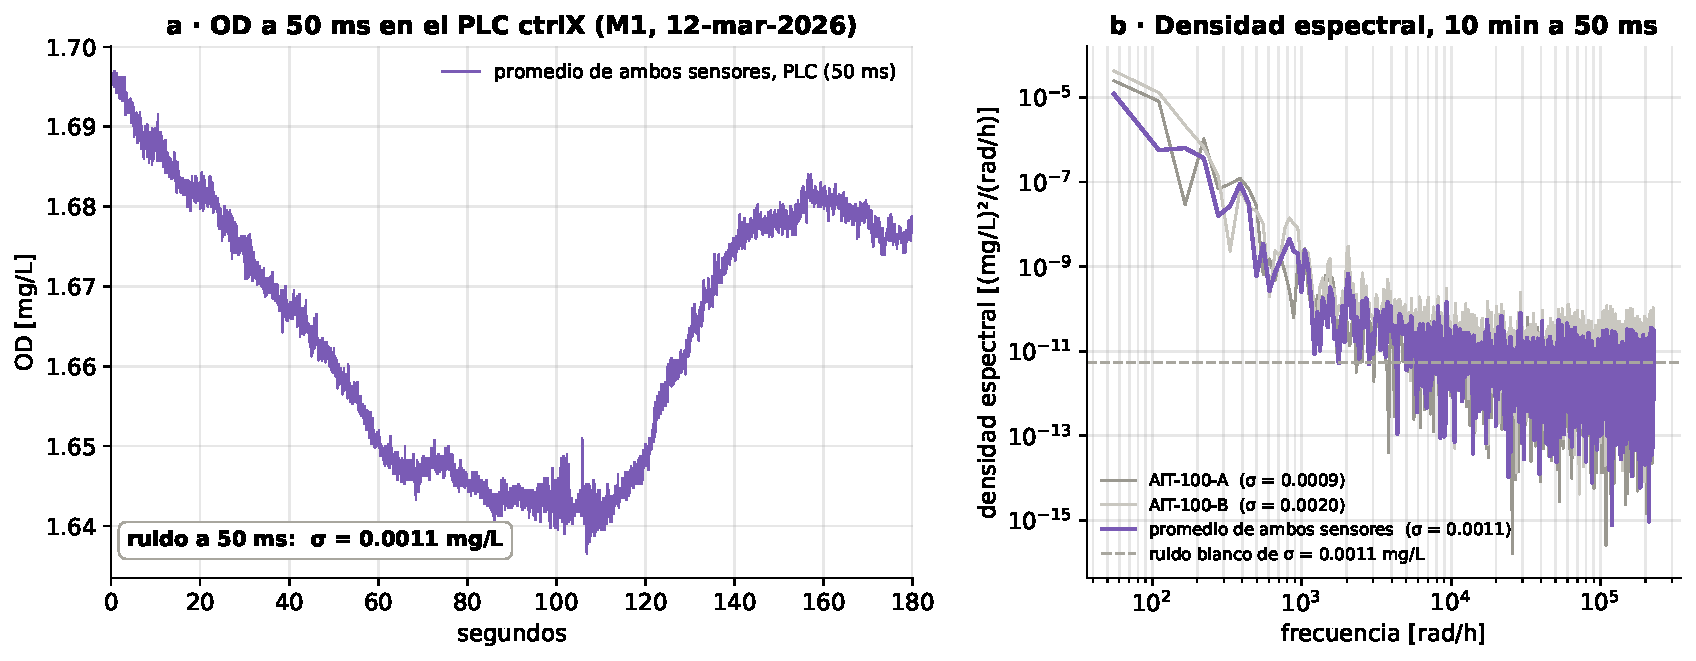
\includegraphics[width=\linewidth]{ident_18_ruido_ctrlx.pdf}
    \caption[Ruido del sensor medido a 50 ms]{Ruido del sensor de OD medido con
    el PLC ctrlX en M1, en el ensayo del 12 de marzo de 2026. (a) Tres minutos
    del promedio de ambos sensores a 50~ms con su $\sigma$. (b) Densidad
    espectral de los últimos 10~min, de cada sensor y de su promedio, con el
    nivel de un ruido blanco de la misma $\sigma$.}
    \label{fig:ident_ruido}
\end{figure}

% ----------------------------------------------------------------------------
\subsection{Planta nominal}
\label{sec:ident_planta_diseno}

Los controladores se diseñan sobre una sola planta nominal: el primer orden y con
retardo como parámetro de validación, Ecuación~\eqref{eq:ident_planta_diseno} con $k_{dc} = 0{,}05$~mg/(L$\cdot$\%),
$\tau = 20$~min y $\theta = 50$~s, es decir,

\begin{equation}
G_p(s) = \frac{0{,}05}{1200\,s + 1}\,e^{-50\,s},
\label{eq:ident_planta_diseno}
\end{equation}

o, en la forma de cadena de integradores del ADRC \eqref{eq:car_b0}, donde $\theta$ no se toma para el
diseño, pero sí para validar la robustez del sistema, con los márgenes de fase y de ganancia, y verificar
que pueda sostener este retardo, y recordar que parte de la dinámica de la planta quedará embebida dentro de la perturbación total.


\begin{equation}
\begin{aligned}
\dot{y}(t) &= \bar{\xi}(t) + b_0\, u(t), \qquad \bar{\xi}(t)  \leftarrow -\frac{y(t)}{\tau}, \\
b_0 &= \frac{k_{dc}}{\tau},
\end{aligned}
\end{equation}

Para que un mismo controlador sirva en los dos módulos, se toma
$k_{dc} = 0{,}05$~mg/(L$\cdot$\%), que queda entre los escalones de M2 y
los de M3 (Figura~\ref{fig:ident_validacion}), y $\tau = 20$~min, cerca de la
mediana de los escalones. Con ellos, el controlador usa
$\bo = k_{dc}/\tau = 0{,}15$~mg/(L$\cdot$h$\cdot$\%). Para revisar la robustez, la
planta se varía en los rangos intercuartílicos de M2 y M3: $k_{dc}$ entre $0{,}022$
y $0{,}109$~mg/(L$\cdot$\%), $\tau$ entre $11$ y $40$~min y $\theta$ entre $0$ y
$60$~s (Sección~\ref{sec:ident_retardo}). La Figura~\ref{fig:ident_planta_diseno}
muestra la respuesta de la planta nominal a un escalón de 0 a 40~\% en $u$, el
que sostiene los $2{,}0$~mg/L.

\begin{figure}[H]
    \centering
    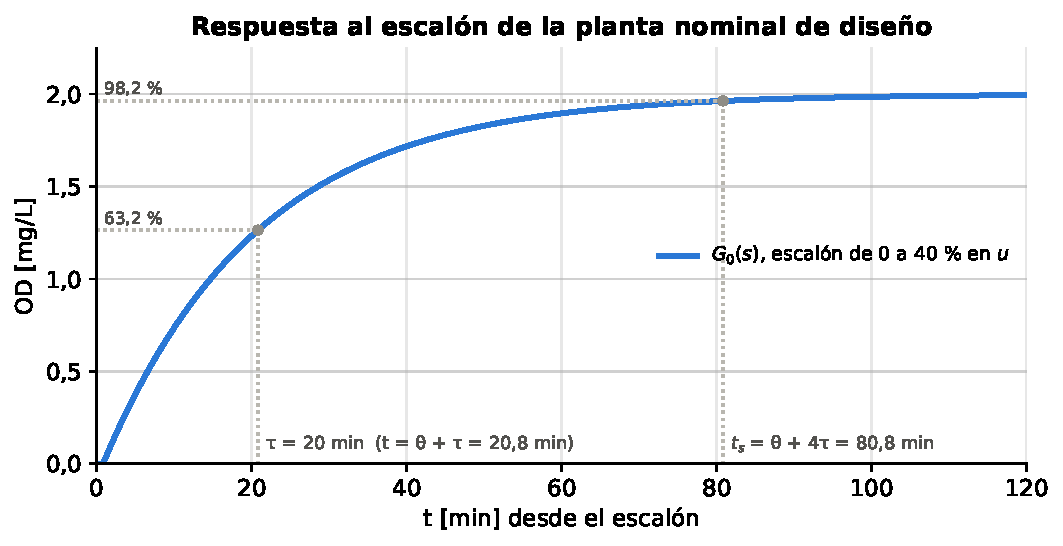
\includegraphics[width=0.85\linewidth]{ident_20_planta_diseno.pdf}
    \caption[Respuesta al escalón de la planta nominal de diseño]{Respuesta de
    la planta nominal de diseño \eqref{eq:ident_planta_diseno} a un escalón de
    0 a 40~\% en la señal de control. Las líneas punteadas grises marcan la
    constante de tiempo (63,2~\% del cambio) y el tiempo de asentamiento,
    $t_s = \theta + 4\,\tau$ (98,2~\% del cambio).}
    \label{fig:ident_planta_diseno}
\end{figure}

% ----------------------------------------------------------------------------
\subsection{Resumen de los parámetros identificados}
\label{sec:ident_resumen}

La Tabla~\ref{tab:ident_resumen} reúne los rangos de todo lo caracterizado en
esta sección: la dinámica de la planta para M2 y M3, con todas las ventanas
ARX, y la planta nominal de diseño, común a los dos módulos. Ahora bien, el
retardo, entre 0 y 60~s, es pequeño frente a
esa dinámica. Por ende, el controlador tiene que funcionar en todos estos
rangos con una sola sintonía, que es justamente lo que se busca con el ADRC.
Además, el espectro de la perturbación indica que casi toda su energía (95~\%)
está por debajo de unos 12~rad/h, lo que fija el mínimo del ancho de banda
del observador $\wo$; el máximo lo ponen el ruido de la medida y el retardo.

\begin{table}[H]
\centering
\caption{Resumen de la caracterización. La dinámica de la planta se da para
M2 y M3; el resto, para M2.}
\label{tab:ident_resumen}
\small
\renewcommand{\arraystretch}{1.15}
\begin{tabular}{llc}
\toprule
\textbf{Magnitud} & \textbf{Condición} & \textbf{Rango} \\
\midrule
\multicolumn{3}{l}{\emph{Dinámica de la planta, M2}} \\
$K$ [mg/(L$\cdot$\%)] & todas las ventanas, rango intercuartílico & 0,0077 -- 0,0342 \\
$\tau$ [min] & todas las ventanas, rango intercuartílico & 11 -- 26 \\
$\bo$ [mg/(L$\cdot$h$\cdot$\%)] & todas las ventanas, rango intercuartílico & 0,0335 -- 0,107 \\
\midrule
\multicolumn{3}{l}{\emph{Dinámica de la planta, M3}} \\
$K$ [mg/(L$\cdot$\%)] & todas las ventanas, rango intercuartílico & 0,0212 -- 0,109 \\
$\tau$ [min] & todas las ventanas, rango intercuartílico & 15 -- 40 \\
$\bo$ [mg/(L$\cdot$h$\cdot$\%)] & todas las ventanas, rango intercuartílico & 0,0816 -- 0,224 \\
\midrule
\multicolumn{3}{l}{\emph{Planta nominal de diseño (M2 y M3)}} \\
$k_{dc}$ [mg/(L$\cdot$\%)] / $\tau$ [min] / $\theta$ [s] & planta nominal (Sección~\ref{sec:ident_planta_diseno}) & 0,05 / 20 / 50 \\
$\bo$ de diseño [mg/(L$\cdot$h$\cdot$\%)] & $k_{dc}/\tau$ & 0,15 \\
\midrule
\multicolumn{3}{l}{\emph{Retardo}} \\
$\theta$ [s] & rango de diseño (medido en M1: 39 y 50~s el ideal) & 0 -- 60 \\
\midrule
\multicolumn{3}{l}{\emph{Ruido del sensor} [mg/L]} \\
$\sigma$ del OD promedio & traza del PLC a 50~ms, M1 & 0,0011 \\
\midrule
\multicolumn{3}{l}{\emph{Caudal de entrada de M2} [L/s]} \\
Entrada (FIT-101) & media / variación del ciclo diario & 34 / 9,4 \\
\quad desviación respecto al ciclo & $\sigma$, robusta & 13,6 \\
\midrule
\multicolumn{3}{l}{\emph{Perturbación total} [mg/(L$\cdot$h)]} \\
Nivel $\bar{\xi}_0$ & en $y = 2$~mg/L & $-8{,}49$ \\
Ciclo diario & completo, pico a pico (medianas) & 3,46 \\
Desviación de $\eta$ & $\sigma_\eta$, robusta & 3,75 \\
Constante de tiempo de $\eta$, $\tau_\eta$ [min] & correlación a 1~h & 58 \\
\midrule
\multicolumn{3}{l}{\emph{Espectro de $\bar{\xi}$} [rad/h]} \\
50~\% de la energía & por debajo de & 1,0 \\
90~\% de la energía & por debajo de & 6,0 \\
95~\% de la energía & por debajo de & 12 \\
99~\% de la energía & por debajo de & 56 \\
\bottomrule
\end{tabular}
\end{table}

% ============================================================================
%  Capítulo 6 - Rechazo activo de perturbaciones basado en observador de estados
% ============================================================================
\chapter{ADRC basado en observador de estado extendido (ESO)}
\label{cap:ADRC-ESO}

% estilos de los diagramas de bloques de este capítulo
\tikzset{
  block/.style={draw, thick, fill=white, align=center, minimum height=1cm, minimum width=1cm},
  sum/.style={draw, thick, circle, fill=white, inner sep=0pt, minimum size=0.4cm},
  sgn/.style={font=\footnotesize, inner sep=1pt}
}

En este capítulo se implementa el ADRC con observador de estado extendido
(ESO), con enfoque basado en el error. En \cite{sira2017adrc} el ADRC se presenta
en esta forma general y para mantener la consistencia en todo el capítulo, el
error se define como $e_y = y - r$. Con base en esta teoría se diseña un controlador
ADRC para una planta de primer orden, con un observador de estado extendido y una
perturbación tipo escalón. Además, se evalúan las ventajas de esta arquitectura y
las desventajas que aparecen en su implementación; por ejemplo, la necesidad de
suavizar la referencia a la entrada del controlador, ya sea con un perfil de
transitorios \cite[sec.~6.3]{herbst2024adrc} o con polinomios de Bézier
\cite{sira2017adrc}. El desarrollo del capítulo se guía por el libro de
Sira-Ramírez et al.\ \cite{sira2017adrc}, los libros de Chen
\cite{chen1993analog,chen1999linear}, el libro de Herbst y Madoński
\cite{herbst2024adrc} y artículos de John Cortés-Romero
\cite{rojas2020equivalence,vargas2026microgrids}.



\section{Del lazo realimentado al esquema ADRC basado en el error}
\label{sec:adrc_esquema}

\subsection{Lazo de control realimentado}
\label{sec:adrc_generalidades}

El lazo cerrado con realimentación unitaria es la forma más común de implementar
un lazo de control; su representación en bloques se muestra en la
Figura~\ref{fig:feedbackBlock}.Como el error se define de la siguiente  $e_y = y - r$, igual
que en \cite{sira2017adrc}, a la entrada del controlador llega
$-e_y$. Este esquema es fácilmente identificable en diferentes lazos de control,
e incluso en los diagramas P\&ID, donde se ubican el proceso y el lazo de control
de cada variable.

\begin{figure}[H]
  \centering
  \begin{tikzpicture}[>=Stealth, thick, font=\small,
      blk/.style={draw, thick, minimum width=1.5cm, minimum height=0.9cm},
      suma/.style={draw, thick, circle, minimum size=0.45cm, inner sep=0pt}]
    \node[suma] (sa) at (2.9,0) {};
    \node[blk] (Ca) at (5.7,0) {$C(s)$};
    \node[blk] (Ga) at (9.0,0) {$G(s)$};
    \draw[->] (0.9,0) node[above right] {$r(t)$} -- (sa.west);
    \draw[->] (sa.east) -- node[above] {$-e_y(t)$} (Ca.west);
    \draw[->] (Ca.east) -- node[above] {$u(t)$} (Ga.west);
    \draw[->] (Ga.east) -- (12.2,0) node[above left] {$y(t)$};
    \fill (11.4,0) circle (1.5pt);
    \draw[->] (11.4,0) -- (11.4,-1.1) -- (2.9,-1.1) -- (sa.south);
    \node at ($(sa.west)+(-0.2,0.25)$) {$+$};
    \node at ($(sa.south)+(-0.25,-0.2)$) {$-$};
  \end{tikzpicture}
  \caption[Lazo de control por realimentación del error]{Lazo de control por
  realimentación del error, con $e_y = y - r$.}
  \label{fig:feedbackBlock}
\end{figure}



\subsection{Esquema basado en el error}
\label{EsquemaError}

Ahora bien, lo que se busca es mantener esta arquitectura clásica de
realimentación, pero diseñando el controlador con el enfoque del ADRC con
observador de estado extendido. Es decir, se diseña un observador que estime la
perturbación para cancelarla de forma aditiva, manteniendo la estructura del
controlador clásico: un bloque de control que recibe el error y entrega la señal
de control $u$. La idea del observador de estado extendido se presenta en la
Figura~\ref{fig:observador}: su salida son los estados estimados, $\hat{e}_y$ y
$\hat{\xi}$. Además, como en todo observador de Luenberger, es necesario
realimentarle también la señal de control, en este caso la normalizada $u_0$
\cite{chen1993analog}.

\begin{figure}[H]
  \centering
  \begin{tikzpicture}[every path/.style={thick}]
    \node[block, minimum width=2.6cm, minimum height=2cm] (obs) at (0,0) {obs};
    \draw[->] (-2.8,0.5)  node[above right] {$e_y(t)$} -- (obs.west |- 0,0.5);
    \draw[->] (-2.8,-0.5) node[above right] {$u_0(t)$} -- (obs.west |- 0,-0.5);
    \draw[->] (obs.east) -- (2.8,0) node[above left] {$\widehat{\mathbf{X}}(t)$};
  \end{tikzpicture}
  \caption{Representación en bloque del observador de estados.}
  \label{fig:observador}
\end{figure}


Para conservar la estructura clásica, se plantea además una ley de control
linealizante que, a partir de los estados extendidos, genera una señal $u$ capaz
de rechazar la perturbación e imponer la dinámica deseada en lazo cerrado. La
estructura completa se presenta en la Figura~\ref{fig:adrc} y se desarrolla en
el resto de este capítulo.
\begin{figure}[H]
  \centering
  \resizebox{\textwidth}{!}{%
  \begin{tikzpicture}[every path/.style={thick}]

    % --- Nodos principales ---
    \node[sum] (s1) at (1.2,0) {};

    \node[block, minimum width=3.8cm, minimum height=1.9cm] (obs) at (5.0,-0.4)
      {$\mathbf{A}_o\widehat{\mathbf{X}}(t) + \mathbf{B}_o \mathbf{u}_t(t)$ \\[10pt] $\mathbf{C}_o\widehat{\mathbf{X}}(t) + \mathbf{D}_o \mathbf{u}_t(t)$};
    \node[above=1pt of obs] {Observador};

    \node[block, minimum size=9mm] (K) at (8.45,0) {$-\mathbf{K}$};
    \coordinate (u0) at (9.7,0);
    \node[block, minimum size=9mm] (ib) at (10.95,0) {$1/b_0$};
    \coordinate (u) at (12.2,0);

    \node[sum] (s2) at (13.0,0) {};

    \node[block, minimum width=3.2cm, minimum height=1.9cm] (plant) at (16.3,0)
      {$\mathbf{A}_g \mathbf{x}_g(t) + \mathbf{B}_g \bar{u}(t)$ \\[10pt] $\mathbf{C}_g \mathbf{x}_g(t) + \mathbf{D}_g \bar{u}(t)$};

    \coordinate (yb) at (18.5,0);

    % --- Recuadro ADRC ---
    \draw[red, dashed, thick] (2.4,1.6) rectangle (11.8,-2.3);
    \node[below left] at (11.8,1.6) {ADRC};

    % --- Señales ---
    \draw[->] (-0.3,0) node[above right] {$r(t)$} -- (s1.west);
    \node[sgn] at ($(s1.west)+(-0.15,0.25)$) {$-$};

    \draw[->] (s1.east) -- node[above, pos=0.4] {$e_y(t)$} (obs.west |- s1);
    \draw[->] (obs.east |- K) -- node[above] {$\widehat{\mathbf{X}}(t)$} (K.west);

    \draw (K.east) -- (u0) node[above] {$u_0(t)$};
    \draw[->] (u0) -- (ib.west);
    \fill (u0) circle (1.5pt);
    \draw (ib.east) -- (u) node[above] {$u(t)$};
    \draw[->] (u) -- (s2.west);
    \node[sgn] at ($(s2.west)+(-0.2,0.25)$) {$+$};

    \draw[->] (u0) -- (u0 |- 0,-1.9) -- (2.75,-1.9) node[above right] {$u_0(t)$}
              -- (2.75,-0.85) -- (obs.west |- 0,-0.85);

    \draw[->] (s2 |- 0,1.6) node[above] {$\varepsilon(t)$} -- (s2.north);
    \node[sgn] at ($(s2.north)+(-0.25,0.2)$) {$+$};

    \draw[->] (s2.east) -- node[above] {$\bar{u}(t)$} (plant.west);

    \draw (plant.east) -- (yb);
    \draw[->] (yb) -- (19.6,0) node[above left] {$y(t)$};
    \fill (yb) circle (1.5pt);

    \draw[->] (yb) -- (18.5,-2.9) -- (1.2,-2.9) -- (s1.south);
    \node[sgn] at ($(s1.south)+(-0.25,-0.15)$) {$+$};
    \node[right] at ($(s1.south)+(0,-0.45)$) {$y(t)$};

  \end{tikzpicture}%
  }
  \caption{Esquema de control ADRC con observador de estados y realimentación de la salida. El
    observador recibe $\mathbf{u}_t = [\,e_y \;\; u_0\,]^{\top}$, y $b_0$ aparece solo al
    pasar de $u_0$ a la orden física $u$.}
  \label{fig:adrc}
\end{figure}
\section{Diseño en tiempo continuo}
\label{sec:ContinuosTime}

El diseño se plantea primero para una planta de orden $n$ y una perturbación
descrita por un modelo interno de orden $m$; al final se particulariza al caso
del oxígeno disuelto: planta de primer orden y perturbación constante a tramos.

%--------------------------------------------------------------------
\subsection{Planteamiento en términos del error}
\label{subsec:error}
Aquí se hacen unos cambios con respecto al esquema clásico del ADRC para pasarlo a un esquema sobre
el error de seguimiento. Para llegar a él se parte de la planta de diseño
\eqref{eq:ident_planta_diseno} sin el retardo, $\theta = 0$, porque este no se toma para el diseño
sino para validar la robustez (Sección~\ref{sec:ident_planta_diseno}):
\begin{equation}
G_p(s) = \frac{Y(s)}{U(s)} = \frac{k_{dc}}{\tau s + 1} = \frac{0{,}05}{1200\,s + 1} .
\label{eq:planta_sin_retardo}
\end{equation}
Con una perturbación $\varepsilon(t)$ a la entrada, en las mismas unidades de $u$, la planta en el
tiempo es
\begin{equation}
\tau\,\dot{y}(t) + y(t) = k_{dc}\bigl(u(t) + \varepsilon(t)\bigr)
\quad\Longrightarrow\quad
\dot{y}(t) = b_0\left(u(t) + \varepsilon(t) - \frac{y(t)}{k_{dc}}\right),
\qquad b_0 = \frac{k_{dc}}{\tau} .
\end{equation}
La dinámica que sobra de la planta, el término $-y/k_{dc}$, se mete dentro de una perturbación
equivalente a la entrada,
\begin{equation}
\dot{y}(t) = b_0\bigl(u(t) + \bar{\varepsilon}(t)\bigr),
\qquad
\bar{\varepsilon}(t) = \varepsilon(t) - \frac{y(t)}{k_{dc}},
\label{eq:planta_eps_bar}
\end{equation}
y la planta queda como un integrador puro con ganancia de entrada
$b_0 = 0{,}05/1200 = 4{,}17\times10^{-5}$~mg/(L$\cdot$s$\cdot$\%), es decir,
$0{,}15$~mg/(L$\cdot$h$\cdot$\%) \eqref{eq:car_b0}. Si la perturbación se lleva al lado de la salida,
$\bar{\xi}(t) = b_0\,\bar{\varepsilon}(t)$, y para una planta de orden $n$ con ganancia de entrada
aproximada $b_0$ (cadena de integradores) la forma general es:
\begin{equation}
y^{(n)}(t) = b_0\,u(t) + \bar{\xi}(t),
\label{eq:planta_n}
\end{equation}
donde $\bar{\xi}(t)$ agrupa las perturbaciones externas, la dinámica no modelada y
el error en la ganancia de entrada. Con la referencia $r(t) = y^*(t)$, se define el
error de seguimiento
\begin{equation}
e_y(t) = y(t) - y^*(t) .
\end{equation}
Restando $y^{*(n)}(t)$ en ambos lados de \eqref{eq:planta_n} se obtiene
\begin{equation}
e_y^{(n)}(t) = b_0\,u(t) + \bigl(\bar{\xi}(t) - u^*(t)\bigr) = b_0\,u(t) + \xi(t),
\qquad u^*(t) = y^{*(n)}(t),
\label{eq:error_n}
\end{equation}
donde $u^*(t)$ es la señal de control necesaria para compensar la $n$-ésima
derivada de la referencia, y $\xi(t) = \bar{\xi}(t) - u^*(t)$ es la perturbación total vista desde el
error. Definiendo la señal de control normalizada $u_0(t) = b_0\,u(t)$, la dinámica del
error queda como una cadena de $n$ integradores excitada por $u_0(t) + \xi(t)$:
\begin{equation}
e_y^{(n)}(t) = u_0(t) + \xi(t) .
\label{eq:error_norm}
\end{equation}
La ganancia $b_0$ aparece una sola vez, al pasar a la orden física
$u(t) = u_0(t)/b_0$; si $b_0 = 1$, ambas señales coinciden. Desde este punto de vista, la ley de control es una
linealización entrada-salida: elimina la perturbación y la ganancia de entrada,
e impone al error una dinámica que cumpla con el diseño.
 
%--------------------------------------------------------------------
\subsection{Modelo de la planta}
\label{subsec:planta}
 
Con el vector de estados
\begin{equation}
\mathbf{x}_p(t) =
\begin{bmatrix} e_y(t) & \dot{e}_y(t) & \cdots & e_y^{(n-1)}(t) \end{bmatrix}^{\top}
\in \mathbb{R}^{n},
\end{equation}
la ecuación \eqref{eq:error_norm} en espacio de estados es
\begin{equation}
\dot{\mathbf{x}}_p(t) = \mathbf{A}_p\,\mathbf{x}_p(t) + \mathbf{B}_p\bigl(u_0(t) + \xi(t)\bigr),
\qquad
e_y(t) = \mathbf{C}_p\,\mathbf{x}_p(t),
\end{equation}
con
\begin{equation}
  \begin{aligned}
  \mathbf{A}_p &=
  \begin{bmatrix}
  0 & 1 & 0 & \cdots & 0 \\
  0 & 0 & 1 & \cdots & 0 \\
  \vdots & \vdots & \vdots & \ddots & \vdots \\
  0 & 0 & 0 & \cdots & 1 \\
  0 & 0 & 0 & \cdots & 0
  \end{bmatrix}_{n \times n}
  & \qquad
  \mathbf{B}_p &=
  \begin{bmatrix}
  0 \\ 0 \\ \vdots \\ 0 \\ 1
  \end{bmatrix}_{n \times 1} \\[1.5em]
  \mathbf{C}_p &=
  \begin{bmatrix}
  1 & 0 & \cdots & 0
  \end{bmatrix}_{1 \times n}
  & \qquad
  \mathbf{D}_p &= 0
  \end{aligned}
\end{equation}
Es decir, con la entrada normalizada, la planta vista desde el error es una
cadena de $n$ integradores, $1/s^{n}$, sea cual sea la planta
(Figura~\ref{fig:cadena_integradores}): todo lo que
la diferencia de ese modelo queda dentro de $\xi$. Si se trabaja con $u$ en lugar de
$u_0$, la ganancia $b_0$ debe incluirse en la última componente de
$\mathbf{B}_p$, ya que en esta forma canónica la entrada solo actúa sobre la
última ecuación.

\begin{figure}[H]
  \centering
  \begin{tikzpicture}[every path/.style={thick}]
    \node[sum] (s) at (1.8,0) {};
    \node[block, minimum size=1.2cm] (i1) at (4.3,0) {$\dfrac{1}{s}$};
    \node[block, minimum size=1.2cm] (i2) at (7.4,0) {$\dfrac{1}{s}$};
    \node (dots) at (9.9,0) {$\cdots$};
    \node[block, minimum size=1.2cm] (i3) at (12.2,0) {$\dfrac{1}{s}$};

    \draw[->] (0,0) node[above right] {$u_0(t)$} -- (s.west);
    \node[sgn] at ($(s.west)+(-0.2,-0.25)$) {$+$};
    \draw[->] (1.8,1.4) node[above] {$\xi(t)$} -- (s.north);
    \node[sgn] at ($(s.north)+(-0.25,0.2)$) {$+$};

    \draw[->] (s.east) -- node[above] {$e_y^{(n)}(t)$} (i1.west);
    \draw[->] (i1.east) -- node[above] {$e_y^{(n-1)}(t)$} node[below] {$x_n(t)$} (i2.west);
    \draw[->] (i2.east) -- node[above] {$e_y^{(n-2)}(t)$} node[below] {$x_{n-1}(t)$} (dots.west);
    \draw[->] (dots.east) -- node[above] {$\dot{e}_y(t)$} node[below] {$x_2(t)$} (i3.west);
    \draw[->] (i3.east) -- node[below, pos=0.4] {$x_1(t)$} (14.6,0) node[above left] {$e_y(t)$};
  \end{tikzpicture}
  \caption[Planta vista desde el error: cadena de integradores]{Planta vista
    desde el error: cadena de $n$ integradores excitada por $u_0 + \xi$. Las
    señales entre integradores son los estados de $\mathbf{x}_p$.}
  \label{fig:cadena_integradores}
\end{figure}

%--------------------------------------------------------------------
\subsection{Modelo interno de la perturbación}
\label{subsec:modelo_interno}

La perturbación $\xi$ puede describirse con un modelo interno de
orden $m$, definido por el polinomio
\begin{equation}
p_{\xi}(s) = s^{m} + \gamma_{m-1}s^{m-1} + \cdots + \gamma_1 s + \gamma_0 ,
\end{equation}
de modo que en el tiempo se tiene:
\begin{equation}
p_{\xi}(\xi,t) = \xi^{(m)}(t) + \gamma_{m-1}\,\xi^{(m-1)}(t) + \cdots
+ \gamma_1\,\dot{\xi}(t) + \gamma_0\,\xi(t) ,
\label{eq:pMI}
\end{equation}
y, despejando la derivada de mayor orden, se obtiene la ecuación diferencial del
último estado del modelo de la perturbación:
\begin{equation}
\xi^{(m)}(t) = -\gamma_{m-1}\,\xi^{(m-1)}(t) - \cdots
- \gamma_1\,\dot{\xi}(t) - \gamma_0\,\xi(t) + p_{\xi}(\xi,t),
\label{eq:pMI2}
\end{equation}
donde $p_{\xi}(\xi,t)$ es el residuo, que es nulo cuando $\xi(t)$ pertenece
exactamente a la estructura de señales que genera el modelo interno. El vector de
estados de la perturbación se construye con $\xi$ y sus derivadas,
\begin{equation}
\mathbf{x}_{\xi}(t) =
\begin{bmatrix} \xi(t) & \dot{\xi}(t) & \cdots & \xi^{(m-1)}(t) \end{bmatrix}^{\top}
\in \mathbb{R}^{m},
\end{equation}
y su representación en espacio de estados es
\begin{equation}
\dot{\mathbf{x}}_{\xi}(t) = \mathbf{A}_{\xi}\,\mathbf{x}_{\xi}(t) + \mathbf{B}_{\xi}\,p_{\xi}(\xi,t),
\qquad
\xi(t) = \mathbf{C}_{\xi}\,\mathbf{x}_{\xi}(t),
\end{equation}
con
\begin{equation}
  \begin{aligned}
  \mathbf{A}_{\xi} &=
  \begin{bmatrix}
  0 & 1 & 0 & \cdots & 0 \\
  0 & 0 & 1 & \cdots & 0 \\
  \vdots & \vdots & \vdots & \ddots & \vdots \\
  0 & 0 & 0 & \cdots & 1 \\
  -\gamma_0 & -\gamma_1 & -\gamma_2 & \cdots & -\gamma_{m-1}
  \end{bmatrix}_{m \times m}
  & \qquad
  \mathbf{B}_{\xi} &=
  \begin{bmatrix}
  0 \\ 0 \\ \vdots \\ 0 \\ 1
  \end{bmatrix}_{m \times 1} \\[1.5em]
  \mathbf{C}_{\xi} &=
  \begin{bmatrix}
  1 & 0 & \cdots & 0
  \end{bmatrix}_{1 \times m}
  & &
  \end{aligned}
\end{equation}
Se usa el caso más sencillo en ADRC, en el que todos los
coeficientes $\gamma_i = 0$: el modelo interno es una cadena de $m$ integradores
($1/s^{m}$) y $p_{\xi}(\xi,t) = \xi^{(m)}(t)$. Con esta estructura el observador puede seguir
señales polinomiales: escalones ($m = 1$), rampas ($m = 2$), y así
sucesivamente. Ahora bien, si se escoge la estructura adecuada, el modelo interno
también puede representar senoidales o señales periódicas.

\paragraph{Modelo interno genérico.} Si el modelo de la perturbación tiene polos
en $\lambda_1$, $\sigma \pm j\omega$ y $\lambda_2$, su matriz puede escribirse en
forma de Jordan real, con un bloque por cada polo real y un bloque de
$2 \times 2$ por cada par complejo, como la presenta Chen
\cite[sec.~4.3.1]{chen1999linear}:
\begin{equation}
\mathbf{A}_{\xi} =
\begin{bmatrix}
\lambda_1 & 0 & 0 & 0 \\
0 & \sigma & \omega & 0 \\
0 & -\omega & \sigma & 0 \\
0 & 0 & 0 & \lambda_2
\end{bmatrix}.
\label{eq:modelo_interno_jordan}
\end{equation}
Es la misma dinámica que la forma compañera anterior con
$p_{\xi}(s) = (s - \lambda_1)\bigl[(s - \sigma)^2 + \omega^2\bigr](s - \lambda_2)$,
escrita en otra base: las dos se relacionan por una transformación de similitud.
En esta forma, $\mathbf{C}_{\xi}$ combina los modos, por ejemplo
$\mathbf{C}_{\xi} = [\,1 \;\; 1 \;\; 0 \;\; 1\,]$. Una senoidal de frecuencia
conocida $\omega$ corresponde a $\sigma = 0$ (polos en $\pm j\omega$); para una
señal periódica se necesita un bloque de $2 \times 2$ por cada armónico que se
quiera rechazar ($\omega, 2\omega, 3\omega, \dots$). Un polo repetido en cero, en cambio, da un
bloque de Jordan con unos sobre la diagonal, que es la cadena de integradores de
los escalones y las rampas. 

 
%--------------------------------------------------------------------
\subsection{Sistema aumentado}
\label{subsec:aumentado}

Al sustituir $\xi(t) = \mathbf{C}_{\xi}\,\mathbf{x}_{\xi}(t)$ en el modelo de la
planta, la planta y el modelo interno quedan en un solo sistema de orden $n+m$,
el sistema aumentado o extendido, cuyos estados estimará después el observador:
\begin{equation}
  e_y^{(n)}(t) = u_0(t) + \xi(t) = u_0(t) + \mathbf{C}_{\xi}\,\mathbf{x}_{\xi}(t),
\end{equation}
con el vector de estados
\begin{equation}
\mathbf{X}(t) =
\begin{bmatrix} \mathbf{x}_p(t) \\ \mathbf{x}_{\xi}(t) \end{bmatrix}
=
\begin{bmatrix} e_y(t) & \cdots & e_y^{(n-1)}(t) & \xi(t) & \cdots & \xi^{(m-1)}(t) \end{bmatrix}^{\top}
\in \mathbb{R}^{n+m},
\end{equation}
la dinámica, estado por estado, es
\begin{equation}
\underbrace{
\begin{aligned}
\dot{x}_1(t) &= x_2(t) \\
&\;\;\vdots \\
\dot{x}_{n-1}(t) &= x_n(t) \\
\dot{x}_n(t) &= x_{n+1}(t) + u_0(t)
\end{aligned}}_{\text{planta: } x_1,\,\dots,\,x_n}
\qquad\quad
\underbrace{
\begin{aligned}
\dot{x}_{n+1}(t) &= x_{n+2}(t) \\
&\;\;\vdots \\
\dot{x}_{n+m-1}(t) &= x_{n+m}(t) \\
\dot{x}_{n+m}(t) &= -\textstyle\sum_{i=0}^{m-1}\gamma_i\,x_{n+1+i}(t) + p_{\xi}(\xi,t)
\end{aligned}}_{\text{modelo interno: } x_{n+1},\,\dots,\,x_{n+m}}
\end{equation}
con salida $e_y(t) = x_1(t)$.

\paragraph{Caso $\gamma_i = 0$.} Si todos los coeficientes del modelo interno son
nulos, la suma desaparece y la última ecuación es el polinomio del modelo interno
aplicado a $\xi$:
\begin{equation}
\textstyle\sum_{i=0}^{m-1}\gamma_i\,x_{n+1+i}(t) = 0
\quad\Longrightarrow\quad
\dot{x}_{n+m}(t) = \xi^{(m)}(t) = p_{\xi}(\xi,t) .
\end{equation}

\paragraph{Forma matricial.} Por bloques, las matrices del sistema aumentado son
\begin{equation}
  \begin{aligned}
  \mathbf{A} &=
  \begin{bmatrix}
  \mathbf{A}_p & \mathbf{B}_p\,\mathbf{C}_{\xi} \\
  \mathbf{0}_{m \times n} & \mathbf{A}_{\xi}
  \end{bmatrix}
  & \qquad
  \mathbf{B} &=
  \begin{bmatrix} \mathbf{B}_p \\ \mathbf{0}_{m \times 1} \end{bmatrix} \\[1.5em]
  \mathbf{C} &=
  \begin{bmatrix} \mathbf{C}_p & \mathbf{0}_{1 \times m} \end{bmatrix}
  & \qquad
  \mathbf{E} &=
  \begin{bmatrix} \mathbf{0}_{n \times 1} \\ \mathbf{B}_{\xi} \end{bmatrix}
  \end{aligned}
\label{eq:aumentado_matrices}
\end{equation}
La planta recibe $u_0(t)$ y la perturbación $\xi(t) = x_{n+1}(t)$ en su última ecuación;
por eso el bloque $\mathbf{B}_p\,\mathbf{C}_{\xi}$ es una matriz $n \times m$
con un único uno en la posición $(n,1)$. Desarrolladas, las matrices solo tienen
unos, ceros y los coeficientes del modelo interno:

\begin{recuadro}{Sistema aumentado de orden $n+m$}
\begin{equation}
\dot{\mathbf{X}}(t) = \mathbf{A}\,\mathbf{X}(t) + \mathbf{B}\,u_0(t)
+ \mathbf{E}\,p_{\xi}(\xi,t),
\qquad
e_y(t) = \mathbf{C}\,\mathbf{X}(t) + \mathbf{D}\,u_0(t),
\label{eq:aumentado}
\end{equation}
con
\begin{equation}
\mathbf{A} =
\left[\begin{array}{cccc|cccc}
0 & 1 & \cdots & 0 & 0 & 0 & \cdots & 0 \\
\vdots & \vdots & \ddots & \vdots & \vdots & \vdots & & \vdots \\
0 & 0 & \cdots & 1 & 0 & 0 & \cdots & 0 \\
0 & 0 & \cdots & 0 & 1 & 0 & \cdots & 0 \\ \hline
0 & 0 & \cdots & 0 & 0 & 1 & \cdots & 0 \\
\vdots & \vdots & & \vdots & \vdots & \vdots & \ddots & \vdots \\
0 & 0 & \cdots & 0 & 0 & 0 & \cdots & 1 \\
0 & 0 & \cdots & 0 & -\gamma_0 & -\gamma_1 & \cdots & -\gamma_{m-1}
\end{array}\right]_{(n+m) \times (n+m)}
\end{equation}
\begin{equation}
\mathbf{B} =
\left[\begin{array}{c}
0 \\ \vdots \\ 0 \\ 1 \\ \hline 0 \\ \vdots \\ 0 \\ 0
\end{array}\right]_{(n+m) \times 1}
\qquad
\mathbf{E} =
\left[\begin{array}{c}
0 \\ \vdots \\ 0 \\ 0 \\ \hline 0 \\ \vdots \\ 0 \\ 1
\end{array}\right]_{(n+m) \times 1}
\end{equation}
\begin{equation}
\mathbf{C} =
\left[\begin{array}{cccc|cccc}
1 & 0 & \cdots & 0 & 0 & 0 & \cdots & 0
\end{array}\right]_{1 \times (n+m)}
\qquad
\mathbf{D} = \begin{bmatrix} 0 \end{bmatrix}_{1 \times 1} .
\end{equation}
Las líneas separan las $n$ filas y columnas de la planta de las $m$ del modelo
interno. El uno de $\mathbf{B}$ está en la fila $n$, donde entra $u_0$, y el de
$\mathbf{E}$ en la fila $n+m$, donde entra el residuo $p_{\xi}(\xi,t)$;
$\mathbf{D}$ es de $1 \times 1$ porque hay una sola entrada, $u_0$, y una sola
salida, $e_y$.
\end{recuadro}

%--------------------------------------------------------------------
\subsection{Observador de estado extendido}
\label{subsec:observador}
Se busca estimar los estados del sistema aumentado
\begin{equation}
  \dot{\mathbf{X}}(t) = \mathbf{A}\,\mathbf{X}(t) + \mathbf{B}\,u_0(t)
+ \mathbf{E}\,p_{\xi}(\xi,t),
\qquad
e_y(t) = \mathbf{C}\,\mathbf{X}(t).
\end{equation}
Para ello se utiliza un observador de estado de Luenberger, tal como lo presenta
Chen \cite[sec.~8.4]{chen1999linear}: una copia del sistema aumentado a la que
ingresa $u_0(t)$ y que se corrige con el error de seguimiento, ponderado por la
ganancia $\mathbf{L}$,
\begin{equation}
\dot{\widehat{\mathbf{X}}}(t) = \mathbf{A}\,\widehat{\mathbf{X}}(t)
+ \mathbf{B}\,u_0(t)
+ \mathbf{L}\bigl(e_y(t) - \mathbf{C}\,\widehat{\mathbf{X}}(t)\bigr),
\end{equation}
o, agrupando los términos en $\widehat{\mathbf{X}}(t)$,
\begin{equation}
\dot{\widehat{\mathbf{X}}}(t) =
\bigl(\mathbf{A} - \mathbf{L}\,\mathbf{C}\bigr)\,\widehat{\mathbf{X}}(t)
+ \mathbf{B}\,u_0(t) + \mathbf{L}\,e_y(t) ,
\label{eq:observador}
\end{equation}
con $\mathbf{L} \in \mathbb{R}^{(n+m)\times 1}$.

\paragraph{Matrices del observador.} El observador
\eqref{eq:observador} es un sistema lineal con dos entradas, el error de
seguimiento y la señal de control normalizada, que es el bloque de la
Figura~\ref{fig:adrc}:
\begin{equation}
\begin{aligned}
\dot{\widehat{\mathbf{X}}}(t) &=
\bigl(\mathbf{A} - \mathbf{L}\,\mathbf{C}\bigr)\,\widehat{\mathbf{X}}(t)
+ \begin{bmatrix} \mathbf{L} & \mathbf{B} \end{bmatrix}
\begin{bmatrix} e_y(t) \\ u_0(t) \end{bmatrix}
= \mathbf{A}_o\,\widehat{\mathbf{X}}(t) + \mathbf{B}_o\,\mathbf{u}_t(t), \\
\widehat{\mathbf{X}}(t) &= \mathbf{C}_o\,\widehat{\mathbf{X}}(t) + \mathbf{D}_o\,\mathbf{u}_t(t),
\end{aligned}
\label{eq:observador_bloque}
\end{equation}
con
\begin{equation}
\begin{aligned}
\mathbf{A}_o &= \mathbf{A} - \mathbf{L}\,\mathbf{C}, & \qquad
\mathbf{B}_o &= \begin{bmatrix} \mathbf{L} & \mathbf{B} \end{bmatrix}, & \qquad
\mathbf{u}_t(t) &= \begin{bmatrix} e_y(t) \\ u_0(t) \end{bmatrix}, \\[0.5em]
\mathbf{C}_o &= \mathbf{I}_{n+m}, &
\mathbf{D}_o &= \mathbf{0}_{(n+m) \times 2}. & &
\end{aligned}
\label{eq:observador_matrices}
\end{equation}
La salida del observador es el estado estimado completo, que es lo que recibe la
ley de control.

\paragraph{Dinámica del error de estimación.} Al restar el observador del
sistema aumentado, el error de estimación
$\bar{\mathbf{e}}(t) = \mathbf{X}(t) - \widehat{\mathbf{X}}(t)$ evoluciona como
\begin{equation}
\dot{\bar{\mathbf{e}}}(t)
- \bigl(\mathbf{A} - \mathbf{L}\,\mathbf{C}\bigr)\,\bar{\mathbf{e}}(t)
= \mathbf{E}\,p_{\xi}(\xi,t) .
\end{equation}
En el dominio de Laplace, con condiciones iniciales nulas, la transformada del
residuo es $p_{\xi}(s)\,\xi(s)$, y el error de estimación queda excitado solo por
el residuo del lado derecho:
\begin{equation}
\underbrace{\bigl(s\mathbf{I} - (\mathbf{A} - \mathbf{L}\,\mathbf{C})\bigr)}_{\text{PO}}
\,\bar{\mathbf{e}}(s) = \mathbf{E}\,p_{\xi}(s)\,\xi(s),
\end{equation}
donde el determinante de la matriz PO es el polinomio característico del
observador. En el caso $\gamma_i = 0$, $p_{\xi}(s) = s^{m}$:
\begin{equation}
\underbrace{\bigl(s\mathbf{I} - (\mathbf{A} - \mathbf{L}\,\mathbf{C})\bigr)}_{\text{PO}}
\,\bar{\mathbf{e}}(s) = \mathbf{E}\,s^{m}\,\xi(s).
\end{equation}
Para poder escoger $\mathbf{L}$ y ubicar los polos del observador donde se
desee, el par $(\mathbf{A}, \mathbf{C})$ del sistema aumentado debe ser
observable, es decir, su matriz de observabilidad debe tener rango completo:
\begin{equation}
\operatorname{rank}
\begin{bmatrix}
\mathbf{C} \\ \mathbf{C}\,\mathbf{A} \\ \vdots \\
\mathbf{C}\,\mathbf{A}^{\,n+m-1}
\end{bmatrix} = n+m .
\label{eq:observabilidad}
\end{equation}
En este caso se cumple: con $\gamma_i = 0$ y
$\mathbf{C} = [\,1 \;\; 0 \;\; \cdots \;\; 0\,]$, esa matriz es la identidad.
Si además $\mathbf{L}$ se escoge de modo que $\mathbf{A}_o = \mathbf{A} - \mathbf{L}\,\mathbf{C}$
sea Hurwitz, es decir, que todos sus valores propios tengan parte real
estrictamente negativa, el error de estimación converge a cero cuando $\xi(t)$
pertenece a la dinámica del modelo interno ($p_{\xi}(\xi,t) = 0$) y, en caso
contrario, queda acotado por el residuo. Es decir, $s^{m}$ actúa como un operador
aniquilador: con $m = 1$ (un integrador en el modelo interno) elimina las constantes,
dado que la derivada de una constante es cero; en general, elimina cualquier señal de
grado $m - 1$, y se cumple que
$\lim_{t \to \infty} \bar{\mathbf{e}}(t) = \mathbf{0}$, por lo que el observador
estima exactamente el estado del sistema: el error de seguimiento, $\hat{e}_y$,
y la perturbación, $\hat{\xi}$.


 
%--------------------------------------------------------------------
\subsection{Ley de control}
\label{subsec:ley}
 
\begin{recuadro}{Ley de control para un sistema de orden $n$}
Para un sistema de orden $n$ cuyo modelo es
\begin{equation}
y^{(n)}(t) = \beta\,u(t) + \phi\bigl(y(t), \dot{y}(t), \dots, y^{(n-1)}(t), t\bigr),
\end{equation}
donde $\beta$ es la ganancia de entrada y $\phi$ agrupa la dinámica no deseada y las
perturbaciones, la ley linealizante
\begin{equation}
u(t) = \frac{v(t) - \phi(t)}{\beta}
\end{equation}
cancela $\phi$ e impone $y^{(n)}(t) = v(t)$, con $v(t)$ una entrada virtual
\cite{sira2017adrc}. Para seguir una referencia $y^*(t)$ se elige
\begin{equation}
v(t) = y^{*(n)}(t) - k_{p_n}\,e_y^{(n-1)}(t) - \cdots - k_{p_2}\,\dot{e}_y(t) - k_{p_1}\,e_y(t),
\end{equation}
con lo que el error $e_y = y - y^*$ cumple
\begin{equation}
e_y^{(n)}(t) + k_{p_n}\,e_y^{(n-1)}(t) + \cdots + k_{p_2}\,\dot{e}_y(t) + k_{p_1}\,e_y(t) = 0 .
\label{eq:ley_error_deseado}
\end{equation}
La planta \eqref{eq:planta_n} tiene esta forma con $\beta = b_0$ y $\phi = \bar{\xi}(t)$. En el
esquema basado en el error, \eqref{eq:error_n} la tiene con $e_y$ en lugar de $y$ y $\phi = \xi(t)$.
Como el término de la referencia, $u^*(t) = y^{*(n)}(t)$, ya está dentro de $\xi(t)$, la entrada
virtual ya no lo lleva. Además, las derivadas del error y $\xi(t)$ no se miden, así que se usan
sus estimados, los que entrega el ESO:
\begin{equation}
\begin{gathered}
v(t) = -k_{p_1}\,\hat{e}_y(t) - k_{p_2}\,\hat{\dot{e}}_y(t) - \cdots - k_{p_n}\,\widehat{e}_y^{(n-1)}(t)
= -\mathbf{K}_p\,\hat{\mathbf{x}}_p(t),\\[4pt]
u(t) = \frac{v(t) - \hat{\xi}(t)}{b_0},
\end{gathered}
\end{equation}
y, cuando la estimación converge, se llega a la misma dinámica del error
\eqref{eq:ley_error_deseado}.
\end{recuadro}

En forma matricial,
\begin{equation}
u(t) = \frac{u_0(t)}{b_0}
  = -\frac{1}{b_0}\bigl(\mathbf{K}_p\,\hat{\mathbf{x}}_p(t) + \hat{\xi}(t)\bigr)
  = -\frac{1}{b_0}\,\mathbf{K}\,\widehat{\mathbf{X}}(t),
\label{eq:ley_matricial}
\end{equation}
con
\begin{equation}
\mathbf{K} =
\begin{bmatrix} \mathbf{K}_p & \mathbf{C}_{\xi} \end{bmatrix}
=
\begin{bmatrix} k_{p_1} & k_{p_2} & \cdots & k_{p_n} & 1 & 0 & \cdots & 0 \end{bmatrix} .
\end{equation}
Solo se compensa $\hat{\xi}(t)$ (la primera componente de $\hat{\mathbf{x}}_{\xi}(t)$),
pues es la única que entra en la planta. Los polos de \eqref{eq:ley_error_deseado} se escogen en
la Sección~\ref{subsec:sintonia}.

La Figura~\ref{fig:adrc_ley} muestra cómo se reparte la ley de control dentro del
ADRC: el estado estimado $\widehat{\mathbf{X}}$ se separa en $\hat{\mathbf{x}}_p$,
que se realimenta con $\mathbf{K}_p$, y en $\hat{\mathbf{x}}_{\xi}$, del que
$\mathbf{C}_{\xi}$ extrae la perturbación estimada $\hat{\xi}$; las dos ramas se
restan para formar $u_0 = -\mathbf{K}_p\,\hat{\mathbf{x}}_p - \hat{\xi}$.

\begin{figure}[H]
  \centering
  \resizebox{\textwidth}{!}{%
\begin{tikzpicture}[every path/.style={thick}]
    % --- Camino directo (arriba) ---
    \node[sum] (s1) at (0,0) {};
    \coordinate (ub) at (1.2,0);
    \node[block, minimum size=9mm] (ib) at (2.4,0) {$1/b_0$};
    \node[sum] (s2) at (4.0,0) {};
    \node[block, minimum width=3.6cm, minimum height=1cm] (plant) at (7.0,0)
      {$\mathbf{A}_g\,\mathbf{x}_g(t) + \mathbf{B}_g\,\bar{u}(t)$};
    \node[block, minimum size=1cm] (Cg) at (10.4,0) {$\mathbf{C}_g$};
    \coordinate (yb) at (12.2,0);

    % --- Observador (medio) ---
    \node[block, minimum height=1.1cm] (obs) at (7.0,-2.2)
      {$(\mathbf{A} - \mathbf{L}\,\mathbf{C})\,\widehat{\mathbf{X}}(t) + \mathbf{B}\,u_0(t) + \mathbf{L}\,e_y(t)$};
    \node[sum] (s3) at (12.2,-2.2) {};

    % --- Ganancias (abajo) ---
    \node[block, minimum size=1cm] (Cx) at (2.6,-3.6) {$\mathbf{C}_{\xi}$};
    \node[block, minimum size=1cm] (Kp) at (2.6,-5.0) {$\mathbf{K}_p$};

    % --- Camino directo ---
    \draw (s1.east) -- (ub) node[above] {$u_0(t)$};
    \fill (ub) circle (1.5pt);
    \draw[->] (ub) -- (ib.west);
    \draw[->] (ib.east) -- node[above] {$u(t)$} (s2.west);
    \draw[->] (s2 |- 0,1.2) node[above] {$\varepsilon(t)$} -- (s2.north);
    \draw[->] (s2.east) -- node[above] {$\bar{u}(t)$} (plant.west);
    \draw[->] (plant.east) -- (Cg.west);
    \draw (Cg.east) -- (yb);
    \fill (yb) circle (1.5pt);
    \draw[->] (yb) -- (13.4,0) node[above left] {$y(t)$};

    % --- Error de seguimiento: e_y = y - r ---
    \draw[->] (yb) -- (s3.north);
    \node[sgn] at ($(s3.north)+(0.2,0.2)$) {$+$};
    \draw[->] (13.9,-2.2) node[above left] {$r(t)$} -- (s3.east);
    \node[sgn] at ($(s3.east)+(0.2,0.2)$) {$-$};
    \draw[->] (s3.west) -- node[above] {$e_y(t)$} (obs.east);

    % --- u0 hacia el observador ---
    \draw[->] (ub) -- (ub |- obs.west) -- (obs.west);

    % --- Demux 1 a 2: X_hat -> (x_xi, x_p) ---
    \draw[line width=3pt] (5.4,-3.25) -- (5.4,-5.35);
    \draw[->] (obs.south) -- (7.0,-4.3) -- node[above] {$\widehat{\mathbf{X}}(t)$} (5.48,-4.3);
    \draw[->] (5.32,-3.6) -- node[above] {$\hat{\mathbf{x}}_{\xi}(t)$} (Cx.east);
    \draw[->] (5.32,-5.0) -- node[above] {$\hat{\mathbf{x}}_p(t)$} (Kp.east);

    % --- Perturbacion estimada y estado de la planta hacia el sumador ---
    \draw[->] (Cx.west) -- (0,-3.6) -- node[pos=0.5, left] {$\hat{\xi}(t)$} (s1.south);
    \node[sgn] at ($(s1.south)+(0.25,-0.2)$) {$-$};

    \draw[->] (Kp.west) -- (-1,-5.0) -- (-1,0) -- (s1.west);
    \node[sgn] at ($(s1.west)+(-0.2,0.25)$) {$-$};
\end{tikzpicture}%
  }
  \caption[Ley de control del ADRC: realimentación de estados y compensación de
    la perturbación]{Ley de control del ADRC. El estado estimado se separa en
    $\hat{\mathbf{x}}_p$, que se realimenta con $\mathbf{K}_p$, y en
    $\hat{\mathbf{x}}_{\xi}$, del que $\mathbf{C}_{\xi}$ extrae la perturbación
    estimada $\hat{\xi}$; el observador recibe $u_0$ y el error de seguimiento
    $e_y = y - r$.}
  \label{fig:adrc_ley}
\end{figure}

%--------------------------------------------------------------------
\subsection{Principio de separación}
\label{subsec:separacion}

Se sigue el desarrollo de Chen
\cite[sec.~8.5]{chen1999linear}. El sistema aumentado y el observador, con la
ley de control \eqref{eq:ley_matricial}, que realimenta los estados estimados,
$u_0(t) = -\mathbf{K}\,\widehat{\mathbf{X}}(t)$, son
\begin{equation}
\begin{aligned}
\dot{\mathbf{X}}(t) &= \mathbf{A}\,\mathbf{X}(t) - \mathbf{B}\mathbf{K}\,\widehat{\mathbf{X}}(t) + \mathbf{E}\,p_{\xi}(\xi,t), \\
\dot{\widehat{\mathbf{X}}}(t) &= \bigl(\mathbf{A} - \mathbf{L}\,\mathbf{C}\bigr)\,\widehat{\mathbf{X}}(t)
+ \mathbf{L}\,\mathbf{C}\,\mathbf{X}(t) - \mathbf{B}\mathbf{K}\,\widehat{\mathbf{X}}(t),
\end{aligned}
\end{equation}
y se pueden combinar como otro sistema aumentado:
\begin{equation}
\begin{aligned}
\begin{bmatrix} \dot{\mathbf{X}}(t) \\ \dot{\widehat{\mathbf{X}}}(t) \end{bmatrix}
&=
\begin{bmatrix} \mathbf{A} & -\mathbf{B}\mathbf{K} \\ \mathbf{L}\,\mathbf{C} & \mathbf{A} - \mathbf{L}\,\mathbf{C} - \mathbf{B}\mathbf{K} \end{bmatrix}
\begin{bmatrix} \mathbf{X}(t) \\ \widehat{\mathbf{X}}(t) \end{bmatrix}
+
\begin{bmatrix} \mathbf{E} \\ \mathbf{0}_{(n+m)\times 1} \end{bmatrix} p_{\xi}(\xi,t), \\
e_y(t) &= \begin{bmatrix} \mathbf{C} & \mathbf{0}_{1\times(n+m)} \end{bmatrix}
\begin{bmatrix} \mathbf{X}(t) \\ \widehat{\mathbf{X}}(t) \end{bmatrix}.
\end{aligned}
\end{equation}
El residuo $p_{\xi}(\xi,t)$ no aparece en la ecuación del observador; recuérdese que, en el caso
ideal, este residuo es cero si el modelo interno, que al final actúa como un aniquilador de la
perturbación, se escoge de acuerdo con ella. Ahora bien, utilizando la transformación de
equivalencia $\mathbf{P}$, tendríamos:
\begin{equation}
\mathbf{P} = \begin{bmatrix} \mathbf{I} & \mathbf{0} \\ \mathbf{I} & -\mathbf{I} \end{bmatrix} = \mathbf{P}^{-1},
\qquad
\begin{bmatrix} \mathbf{X}(t) \\ \bar{\mathbf{e}}(t) \end{bmatrix}
=
\begin{bmatrix} \mathbf{I} & \mathbf{0} \\ \mathbf{I} & -\mathbf{I} \end{bmatrix}
\begin{bmatrix} \mathbf{X}(t) \\ \widehat{\mathbf{X}}(t) \end{bmatrix},
\end{equation}
transformación que cambia el estado estimado por el error de estimación,
$\bar{\mathbf{e}}(t) = \mathbf{X}(t) - \widehat{\mathbf{X}}(t)$, se obtiene una
realización equivalente:
\begin{equation}
\begin{aligned}
\begin{bmatrix} \dot{\mathbf{X}}(t) \\ \dot{\bar{\mathbf{e}}}(t) \end{bmatrix}
&=
\begin{bmatrix} \mathbf{A} - \mathbf{B}\mathbf{K} & \mathbf{B}\mathbf{K} \\ \mathbf{0} & \mathbf{A} - \mathbf{L}\,\mathbf{C} \end{bmatrix}
\begin{bmatrix} \mathbf{X}(t) \\ \bar{\mathbf{e}}(t) \end{bmatrix}
+
\begin{bmatrix} \mathbf{E} \\ \mathbf{E} \end{bmatrix} p_{\xi}(\xi,t), \\
e_y(t) &= \begin{bmatrix} \mathbf{C} & \mathbf{0} \end{bmatrix}
\begin{bmatrix} \mathbf{X}(t) \\ \bar{\mathbf{e}}(t) \end{bmatrix}.
\end{aligned}
\label{eq:separacion}
\end{equation}
La transformación de equivalencia no cambia los valores propios, y la nueva
matriz es triangular por bloques: sus valores propios son los de los bloques de
la diagonal, $\mathbf{A} - \mathbf{B}\mathbf{K}$ y $\mathbf{A} - \mathbf{L}\,\mathbf{C}$,
porque el determinante de una matriz triangular por bloques es el producto de los
determinantes de sus bloques diagonales:
\begin{equation}
\det\begin{bmatrix}
s\mathbf{I} - \mathbf{A} + \mathbf{B}\mathbf{K} & -\mathbf{B}\mathbf{K} \\
\mathbf{0} & s\mathbf{I} - \mathbf{A} + \mathbf{L}\,\mathbf{C}
\end{bmatrix}
= \det\bigl(s\mathbf{I} - \mathbf{A} + \mathbf{B}\mathbf{K}\bigr)\,
  \det\bigl(s\mathbf{I} - \mathbf{A} + \mathbf{L}\,\mathbf{C}\bigr).
\end{equation}
Insertar el observador no mueve los polos de la realimentación, ni la
realimentación los del observador. Este es el principio de separación: las
ganancias del lazo externo, $\mathbf{K}$, que fijan la dinámica de la planta, y
las del lazo interno, $\mathbf{L}$, que fijan la del observador, se calculan por
separado.

Para ello, el sistema debe ser controlable y observable, cada condición en la
parte que le corresponde. Seguidamente, con $\mathbf{K} = [\,\mathbf{K}_p \;\; \mathbf{C}_{\xi}\,]$,
el bloque superior derecho de $\mathbf{A} - \mathbf{B}\mathbf{K}$ se anula:
\begin{equation}
\mathbf{A} - \mathbf{B}\mathbf{K} =
\begin{bmatrix} \mathbf{A}_p - \mathbf{B}_p\mathbf{K}_p & \mathbf{B}_p\mathbf{C}_{\xi} - \mathbf{B}_p\mathbf{C}_{\xi} \\ \mathbf{0}_{m\times n} & \mathbf{A}_{\xi} \end{bmatrix}
=
\begin{bmatrix} \mathbf{A}_p - \mathbf{B}_p\mathbf{K}_p & \mathbf{0}_{n\times m} \\ \mathbf{0}_{m\times n} & \mathbf{A}_{\xi} \end{bmatrix},
\end{equation}
es decir, la perturbación ya no está en la dinámica de la planta.
Así, los valores propios de $\mathbf{A} - \mathbf{B}\mathbf{K}$ son los de
$\mathbf{A}_p - \mathbf{B}_p\mathbf{K}_p$, que se escogen con $\mathbf{K}_p$: la única forma de mover los estados de la planta es por medio de esta
ganancia, que es la única que puede reasignar los valores propios del lazo cerrado. Por eso, la
controlabilidad se exige solo al par $(\mathbf{A}_p, \mathbf{B}_p)$: su matriz de
controlabilidad debe tener rango completo,
\begin{equation}
\operatorname{rank}
\begin{bmatrix} \mathbf{B}_p & \mathbf{A}_p\mathbf{B}_p & \cdots & \mathbf{A}_p^{\,n-1}\mathbf{B}_p \end{bmatrix} = n,
\end{equation}
condición que en la cadena de integradores se cumple siempre, porque esa matriz
tiene unos en la antidiagonal y ceros en el resto. La observabilidad, en cambio,
se exige al sistema aumentado completo, $(\mathbf{A}, \mathbf{C})$, con la
condición \eqref{eq:observabilidad}, porque el observador debe reconstruir
también la perturbación. Además, el lazo interno del observador debe ser más
rápido que el lazo externo de control; en otras palabras, el observador debe
tener listas las estimaciones antes de que se imponga la dinámica del lazo
externo.

\subsection{Sintonización}
\label{subsec:sintonia}

Con el principio de separación validado, las ganancias del controlador y las del
observador se obtienen por separado; solo hay que tener presente que, bajo este
enfoque, el observador debe ser más rápido que el controlador. Ambas se puede calcular por 
por asignación de polos: se escogen los polos deseados, se forma su polinomio
característico y las ganancias salen de la fórmula de Ackermann o por ancho de banda dependiendo de el enfoque que le de.


\paragraph{Ganancias del controlador.} Como el par $(\mathbf{A}_p, \mathbf{B}_p)$
es controlable, los valores propios de $\mathbf{A}_p - \mathbf{B}_p\mathbf{K}_p$
se pueden asignar arbitrariamente \cite[teo.~8.3]{chen1999linear}. Con los polos
deseados $\lambda_{c,1}, \dots, \lambda_{c,n}$ y su polinomio característico
\begin{equation}
\Delta_c(s) = (s - \lambda_{c,1}) \cdots (s - \lambda_{c,n})
= s^{n} + \alpha_{c,n-1}\, s^{n-1} + \cdots + \alpha_{c,1}\, s + \alpha_{c,0},
\end{equation}
la fórmula de Ackermann da
\begin{equation}
\mathbf{K}_p =
\begin{bmatrix} 0 & \cdots & 0 & 1 \end{bmatrix}
\begin{bmatrix} \mathbf{B}_p & \mathbf{A}_p\mathbf{B}_p & \cdots & \mathbf{A}_p^{\,n-1}\mathbf{B}_p \end{bmatrix}^{-1}
\Delta_c(\mathbf{A}_p),
\label{eq:ackermann_K}
\end{equation}
con $\Delta_c(\mathbf{A}_p) = \mathbf{A}_p^{\,n} + \alpha_{c,n-1}\mathbf{A}_p^{\,n-1} + \cdots + \alpha_{c,1}\mathbf{A}_p + \alpha_{c,0}\mathbf{I}$.
En la cadena de integradores, las ganancias son directamente los coeficientes del
polinomio,
\begin{equation}
\mathbf{K}_p =
\begin{bmatrix} k_{p_1} & k_{p_2} & \cdots & k_{p_n} \end{bmatrix}
=
\begin{bmatrix} \alpha_{c,0} & \alpha_{c,1} & \cdots & \alpha_{c,n-1} \end{bmatrix} .
\end{equation}
La parte de $\mathbf{K}$ que multiplica al
modelo interno y que no se diseña sino simplemente se estima para ser cancelada: es $\mathbf{C}_{\xi}$, que se usa para obtener $\hat{\xi}$.

\paragraph{Ganancias del observador.} Por dualidad, los valores propios de
$\mathbf{A} - \mathbf{L}\,\mathbf{C}$ se pueden asignar arbitrariamente si
$(\mathbf{A}, \mathbf{C})$ es observable: se calculan las ganancias de
realimentación del par $(\mathbf{A}^{\top}, \mathbf{C}^{\top})$ y se trasponen
\cite[teo.~8.O3]{chen1999linear}, que es lo que hace, por ejemplo,
\texttt{acker(A',C',p)'} en MATLAB. Con los polos deseados del observador y su
polinomio característico
\begin{equation}
\Delta_o(s) = (s - \lambda_{o,1}) \cdots (s - \lambda_{o,n+m})
= s^{n+m} + \alpha_{o,1}\, s^{n+m-1} + \cdots + \alpha_{o,n+m},
\end{equation}
la fórmula de Ackermann dual es
\begin{equation}
\mathbf{L} = \Delta_o(\mathbf{A})
\begin{bmatrix}
\mathbf{C} \\ \mathbf{C}\,\mathbf{A} \\ \vdots \\ \mathbf{C}\,\mathbf{A}^{\,n+m-1}
\end{bmatrix}^{-1}
\begin{bmatrix} 0 \\ \vdots \\ 0 \\ 1 \end{bmatrix} .
\label{eq:ackermann_L}
\end{equation}
Como la matriz de observabilidad es la identidad, $\mathbf{L}$ es la última
columna de $\Delta_o(\mathbf{A})$, y con $\gamma_i = 0$ sus componentes son los
coeficientes del polinomio, $l_i = \alpha_{o,i}$.

\paragraph{Sintonía por ancho de banda.} Si todos los polos del controlador se
ubican en un mismo punto, $-\omega_c$, y todos los del observador en
$-\omega_o$,
\begin{equation}
\Delta_c(s) = (s + \omega_c)^{n}, \qquad \Delta_o(s) = (s + \omega_o)^{n+m},
\label{eq:sintonia_polos}
\end{equation}
la asignación de polos se reduce a la sintonía por ancho de banda de Herbst y
Madoński \cite[tabla~A.1.1]{herbst2024adrc}, con $\omega_c$ el ancho de banda
deseado del lazo cerrado y $\omega_o$ el del observador. Las ganancias son
\begin{equation}
\begin{aligned}
k_{p_i} &= \frac{n!}{(n-i+1)!\,(i-1)!}\,\omega_c^{\,n-i+1}, & i &= 1, \dots, n, \\[0.5em]
l_i &= \frac{(n+m)!}{(n+m-i)!\,i!}\,\omega_o^{\,i}, & i &= 1, \dots, n+m .
\end{aligned}
\label{eq:sintonia_l}
\end{equation}
Herbst y Madoński las presentan para un solo estado extendido ($m = 1$) y
escriben $\omega_o = k_{\mathrm{ESO}}\,\omega_c$, con $k_{\mathrm{ESO}}$ el factor
del ancho de banda del observador respecto al del lazo cerrado. Es decir, se mantiene el orden de la planta
y se trata de estimar la perturbación calculando dónde debe quedar el ancho de banda del observador
para rechazarla adecuadamente.

%--------------------------------------------------------------------
\subsection{Sistema en lazo cerrado}
\label{subsec:lazo_cerrado}

Para simular el lazo, el observador \eqref{eq:observador_bloque} y la ley de
control \eqref{eq:ley_matricial} se conectan con la planta $G(s)$ de la
Figura~\ref{fig:adrc}, que no tiene por qué ser la cadena de integradores del
diseño. En adelante, \emph{planta} es $G(s)$, el sistema que se controla, y
\emph{cadena de integradores}, el modelo con el que se diseñan el observador y la
ley de control; las discrepancias entre las dos son las incertidumbres endógenas
que el ADRC deberá compensar. El estado de la planta es
$\mathbf{x}_g(t) \in \mathbb{R}^{n}$; recibe la orden física $u(t)$ más una
perturbación de entrada $\varepsilon(t)$, en las mismas unidades de $u$, y
$\mathbf{B}_g$ lleva su ganancia:
\begin{equation}
\dot{\mathbf{x}}_g(t) = \mathbf{A}_g\,\mathbf{x}_g(t) + \mathbf{B}_g\bigl(u(t) + \varepsilon(t)\bigr),
\qquad
y(t) = \mathbf{C}_g\,\mathbf{x}_g(t),
\qquad
e_y(t) = \mathbf{C}_g\,\mathbf{x}_g(t) - r(t).
\end{equation}
Recordar que lo que el observador ve como $\xi(t)$ es el efecto de $\varepsilon(t)$ más la
dinámica de $G(s)$ que no es cadena de integradores y $u^*(t)$ \eqref{eq:error_n}. Al sustituir
$u(t) = -\mathbf{K}\,\widehat{\mathbf{X}}(t)/b_0$ en la planta, y
$u_0(t) = -\mathbf{K}\,\widehat{\mathbf{X}}(t)$ y $e_y(t)$ en el observador,
el lazo cerrado, sin saturación del actuador, es
\begin{equation}
\begin{bmatrix} \dot{\mathbf{x}}_g(t) \\ \dot{\widehat{\mathbf{X}}}(t) \end{bmatrix}
=
\begin{bmatrix} \mathbf{A}_g & -\dfrac{1}{b_0}\,\mathbf{B}_g\mathbf{K} \\[0.8em] \mathbf{L}\,\mathbf{C}_g & \mathbf{A} - \mathbf{L}\,\mathbf{C} - \mathbf{B}\mathbf{K} \end{bmatrix}
\begin{bmatrix} \mathbf{x}_g(t) \\ \widehat{\mathbf{X}}(t) \end{bmatrix}
+
\begin{bmatrix} \mathbf{0}_{n \times 1} & \mathbf{B}_g \\ -\mathbf{L} & \mathbf{0}_{(n+m) \times 1} \end{bmatrix}
\begin{bmatrix} r(t) \\ \varepsilon(t) \end{bmatrix}.
\label{eq:lazo_cerrado}
\end{equation}
La ganancia $b_0$ aparece solo en la fila de la planta: el observador trabaja con
el modelo normalizado y recibe $u_0(t)$, no $u(t)$. Con $b_0 = 1$ se dejaría
toda la ganancia dentro del modelo de la planta. Importante tener presente no duplicar la ganancia $b_o$.


%--------------------------------------------------------------------
\section{Caso de estudio: planta de primer orden y perturbación tipo paso (Ejemplo PTAR)}
\label{subsec:caso_n1}

En esta sección se resume el diseño de la Sección~\ref{sec:ContinuosTime} con los
valores del lazo de oxígeno disuelto. La planta es la nominal de diseño
(Sección~\ref{sec:ident_planta_diseno}), un primer orden con
$k_{dc} = 0{,}05$~mg/(L$\cdot$\%) y $\tau = 20$~min.

%--------------------------------------------------------------------
\subsection{Parámetros del diseño}
\label{subsec:caso_parametros}

Con $n = 1$ y $m = 1$ ($\gamma_0 = 0$), los estados del sistema aumentado son
$x_1(t) = e_y(t)$ y $x_2(t) = \xi(t)$:
\begin{equation}
\dot{x}_1(t) = x_2(t) + u_0(t), \qquad \dot{x}_2(t) = \dot{\xi}(t), \qquad u_0(t) = b_0\,u(t) ,
\end{equation}
donde $\dot{\xi}(t)$ es desconocida; en el diseño del observador se supone
$\dot{\xi}(t) = 0$, es decir, una perturbación constante 
\cite[sec.~3.1]{herbst2024adrc}. La ganancia es definida por $b_0 = k_{dc}/\tau$, y los anchos de banda se escogen con la
sintonía de la Sección~\ref{subsec:sintonia}: el controlador cuatro veces más
rápido que el lazo abierto ($\tau_c = \tau/4 = 300$~s,$\omega_c=4\cdot\frac{1}{\tau}$) y el observador cinco veces
más rápido que el controlador; Herbst y Madoński sugieren empezar entre $3$ y $10$ veces
\cite[sec.~3.3]{herbst2024adrc}. La Tabla~\ref{tab:caso_parametros} resume los
valores.

\begin{table}[H]
\centering
\caption{Parámetros del ADRC para el lazo de oxígeno disuelto.}
\label{tab:caso_parametros}
\small
\begin{tabular}{llll}
\toprule
\textbf{Parámetro} & \textbf{Expresión} & \textbf{Valor} & \textbf{En horas} \\
\midrule
Ganancia estática & $k_{dc}$ & $0{,}05$ mg/(L$\cdot$\%) & \\
Constante de tiempo & $\tau$ & $1200$ s & $0{,}33$ h ($20$ min) \\
Ganancia de entrada & $b_0 = k_{dc}/\tau$ & $4{,}17\times10^{-5}$ mg/(L$\cdot$s$\cdot$\%) & $0{,}15$ mg/(L$\cdot$h$\cdot$\%) \\
Ancho de banda del controlador & $\omega_c = 4/\tau$ & $3{,}33\times10^{-3}$ rad/s & $12$ rad/h \\
Ancho de banda del observador & $\omega_o = 5\,\omega_c$ & $0{,}0167$ rad/s & $60$ rad/h \\
\bottomrule
\end{tabular}
\end{table}

%--------------------------------------------------------------------
\subsection{Matrices del sistema}
\label{subsec:caso_matrices}

Al sustituir $n = 1$, $m = 1$ y los valores de la Tabla~\ref{tab:caso_parametros}
en las matrices de la Sección~\ref{sec:ContinuosTime}, se obtienen las de la
Tabla~\ref{tab:caso_matrices}. Para la planta se usa la realización con
$y(t) = x_g(t)$.


\begin{table}[H]
\centering
\caption{Matrices del ADRC para el lazo de oxígeno disuelto ($n = 1$, $m = 1$).}
\label{tab:caso_matrices}
\renewcommand{\arraystretch}{1.6}
\resizebox{\textwidth}{!}{%
\begin{tabular}{lll}
\toprule
\textbf{Sistema} & \textbf{Matrices generales} & \textbf{Valores} \\
\midrule
Cadena de integradores & $\mathbf{A}_p = 0,\ \mathbf{B}_p = 1,\ \mathbf{C}_p = 1,\ \mathbf{D}_p = 0$ & --- \\
Modelo interno & $\mathbf{A}_{\xi} = 0,\ \mathbf{B}_{\xi} = 1,\ \mathbf{C}_{\xi} = 1$ & --- \\
Sistema aumentado &
$\mathbf{A} = \begin{bmatrix} 0 & 1 \\ 0 & 0 \end{bmatrix},\
\mathbf{B} = \begin{bmatrix} 1 \\ 0 \end{bmatrix},\
\mathbf{E} = \begin{bmatrix} 0 \\ 1 \end{bmatrix}$ &
$\mathbf{C} = \begin{bmatrix} 1 & 0 \end{bmatrix},\ \mathbf{D} = 0$ \\
Controlabilidad (planta) &
$\mathcal{C}_p = \begin{bmatrix} \mathbf{B}_p \end{bmatrix}$ &
$\mathcal{C}_p = 1,\ \operatorname{rank}\mathcal{C}_p = 1$ \\
Observabilidad &
$\mathcal{O} = \begin{bmatrix} \mathbf{C} \\ \mathbf{C}\,\mathbf{A} \end{bmatrix}$ &
$\mathcal{O} = \begin{bmatrix} 1 & 0 \\ 0 & 1 \end{bmatrix} = \mathbf{I}_2,\ \operatorname{rank}\mathcal{O} = 2$ \\
Controlador &
$\mathbf{K} = \begin{bmatrix} k_p & 1 \end{bmatrix} = \begin{bmatrix} \omega_c & 1 \end{bmatrix}$ &
$\mathbf{K} = \begin{bmatrix} 3{,}33\times10^{-3} & 1 \end{bmatrix}$ \\
Observador &
$\mathbf{L} = \begin{bmatrix} 2\,\omega_o \\ \omega_o^2 \end{bmatrix},\
\mathbf{A}_o = \begin{bmatrix} -2\,\omega_o & 1 \\ -\omega_o^2 & 0 \end{bmatrix}$ &
$\mathbf{L} = \begin{bmatrix} 0{,}0333 \\ 2{,}78\times10^{-4} \end{bmatrix},\
\mathbf{A}_o = \begin{bmatrix} -0{,}0333 & 1 \\ -2{,}78\times10^{-4} & 0 \end{bmatrix}$ \\
 &
$\mathbf{B}_o = \begin{bmatrix} \mathbf{L} & \mathbf{B} \end{bmatrix},\
\mathbf{C}_o = \mathbf{I}_2,\ \mathbf{D}_o = \mathbf{0}_{2\times 2}$ &
$\mathbf{B}_o = \begin{bmatrix} 0{,}0333 & 1 \\ 2{,}78\times10^{-4} & 0 \end{bmatrix}$ \\
Planta &
$\mathbf{A}_g = -1/\tau,\ \mathbf{B}_g = k_{dc}/\tau,\ \mathbf{C}_g = 1$ &
$\mathbf{A}_g = -8{,}33\times10^{-4},\ \mathbf{B}_g = 4{,}17\times10^{-5}$ \\
\bottomrule
\end{tabular}%
}
\end{table}

Con estos valores, el lazo cerrado \eqref{eq:lazo_cerrado}, con los estados
$x_g(t)$, $\hat{e}_y(t)$ y $\hat{\xi}(t)$, queda
\begin{equation}
\begin{bmatrix} \dot{x}_g(t) \\ \dot{\hat{e}}_y(t) \\ \dot{\hat{\xi}}(t) \end{bmatrix}
=
\begin{bmatrix}
-8{,}33\times10^{-4} & -0{,}0033 & -1 \\
0{,}0333 & -0{,}0367 & 0 \\
2{,}78\times10^{-4} & -2{,}78\times10^{-4} & 0
\end{bmatrix}
\begin{bmatrix} x_g(t) \\ \hat{e}_y(t) \\ \hat{\xi}(t) \end{bmatrix}
+
\begin{bmatrix}
0 & 4{,}17\times10^{-5} \\
-0{,}0333 & 0 \\
-2{,}78\times10^{-4} & 0
\end{bmatrix}
\begin{bmatrix} r(t) \\ \varepsilon(t) \end{bmatrix},
\label{eq:caso_lazo_cerrado}
\end{equation}

\paragraph{Ubicación de los polos.} Las ganancias se calculan asignando los polos (Sección~\ref{subsec:sintonia}) para que el sistema tenga el criterio de los anchos de banda de la tabla~\ref{tab:caso_parametros}: el polo del controlador cuatro veces más rápido
que la planta en lazo abierto, $-\omega_c = -4/\tau$, y los dos del observador
cinco veces más rápidos que el controlador, en $-\omega_o = -5\,\omega_c$. Con
$n = 1$, el polinomio deseado del controlador es $\Delta_c(s) = s + \omega_c$, y
la fórmula de Ackermann \eqref{eq:ackermann_K}, con $\mathbf{A}_p = 0$ y
$\mathbf{B}_p = 1$, da
\begin{equation}
k_p  = \omega_c = 3{,}33\times10^{-3}~\text{s}^{-1}.
\end{equation}
Para el observador, $\Delta_o(s) = (s + \omega_o)^2 = s^2 + 2\omega_o\,s + \omega_o^2$.
Como $\mathbf{A}^2 = \mathbf{0}$ y la matriz de observabilidad es la identidad,
la fórmula dual \eqref{eq:ackermann_L} deja $\mathbf{L}$ de la siguiente forma::
\begin{equation}
\Delta_o(\mathbf{A}) = \mathbf{A}^2 + 2\omega_o\,\mathbf{A} + \omega_o^2\,\mathbf{I}
= \begin{bmatrix} \omega_o^2 & 2\omega_o \\ 0 & \omega_o^2 \end{bmatrix}
\quad\Longrightarrow\quad
\mathbf{L} = \begin{bmatrix} 2\omega_o \\ \omega_o^2 \end{bmatrix}
= \begin{bmatrix} 0{,}0333 \\ 2{,}78\times10^{-4} \end{bmatrix}.
\end{equation}
Las fórmulas de Herbst y Madoński \eqref{eq:sintonia_l}, con $n = m = 1$, dan lo
mismo, $k_{p_1} = \omega_c$, $l_1 = 2\omega_o$ y $l_2 = \omega_o^2$, porque los
polos se ubicaron en un solo punto (polos duplicados): basta conocer los anchos de banda deseados. Por ejemplo, $\omega_o$ quedó
igual a $60$~rad/h, y en la Tabla~\ref{tab:ident_espectro_f} vemos que el $95~\%$ de la energía de la
perturbación está por debajo de $12$~rad/h y el $99~\%$ por debajo de $56$~rad/h, por lo que con este valor casi
toda la perturbación queda dentro de la banda del observador, e incluso se podría bajar un poco más.

\paragraph{Polos con la planta nominal.} Los polos de arriba son los del diseño, utilizando la cadena de integradores.
Con la planta nominal, que no es un integrador
puro, los valores propios del lazo cerrado \eqref{eq:caso_lazo_cerrado} quedan un poco movidos, y se registran en
la Tabla~\ref{tab:caso_polos}: los del observador casi no se mueven y el
del controlador queda un poco más lento, porque el observador no compensa de
forma perfecta la dinámica de la planta, el término $-y/\tau$ que queda dentro de
$\xi$. Herbst y Madoński lo mencionan: el lazo cerrado solo es aproximadamente el
de diseño, porque el lazo interno no es perfecto en la práctica
\cite[ec.~(2.34)]{herbst2024adrc}, y con la cadena de integradores la respuesta
se desvía un poco de la nominal, a una escala muy limitada. Además, la dinámica de la planta real no
se conoce muy bien como para realizar un ajuste; simplemente está dentro de un rango intercuartílico.


\begin{table}[H]
\centering
\caption[Polos del lazo cerrado: diseño y planta nominal]{Polos del lazo cerrado
  del ADRC: los del diseño, con la cadena de integradores, y los que resultan con
  la planta nominal \eqref{eq:caso_lazo_cerrado}.}
\label{tab:caso_polos}
\renewcommand{\arraystretch}{1.3}
\begin{tabular}{lcc}
\toprule
\textbf{Polo} & \textbf{Diseño (cadena de integradores)} & \textbf{Planta nominal} \\
 & [rad/h] & [rad/h] \\
\midrule
Controlador & $-\omega_c = -12{,}0$ & $-10{,}4$ \\
Observador (doble) & $-\omega_o = -60{,}0$ & $-62{,}3$ \\
\bottomrule
\end{tabular}
\end{table}

%--------------------------------------------------------------------
\subsection{Simulación en lazo cerrado}
\label{subsec:caso_simulacion}

La Figura~\ref{fig:adrc_lazo_cerrado} muestra el lazo cerrado con la planta,
sin saturación del actuador. La consigna
sube de $2{,}0$ a $2{,}2$~mg/L en $t = 4000$~s, y en $t = 7000$~s entra una
perturbación de entrada $\varepsilon = -15~\%$.

\begin{figure}[H]
  \centering
  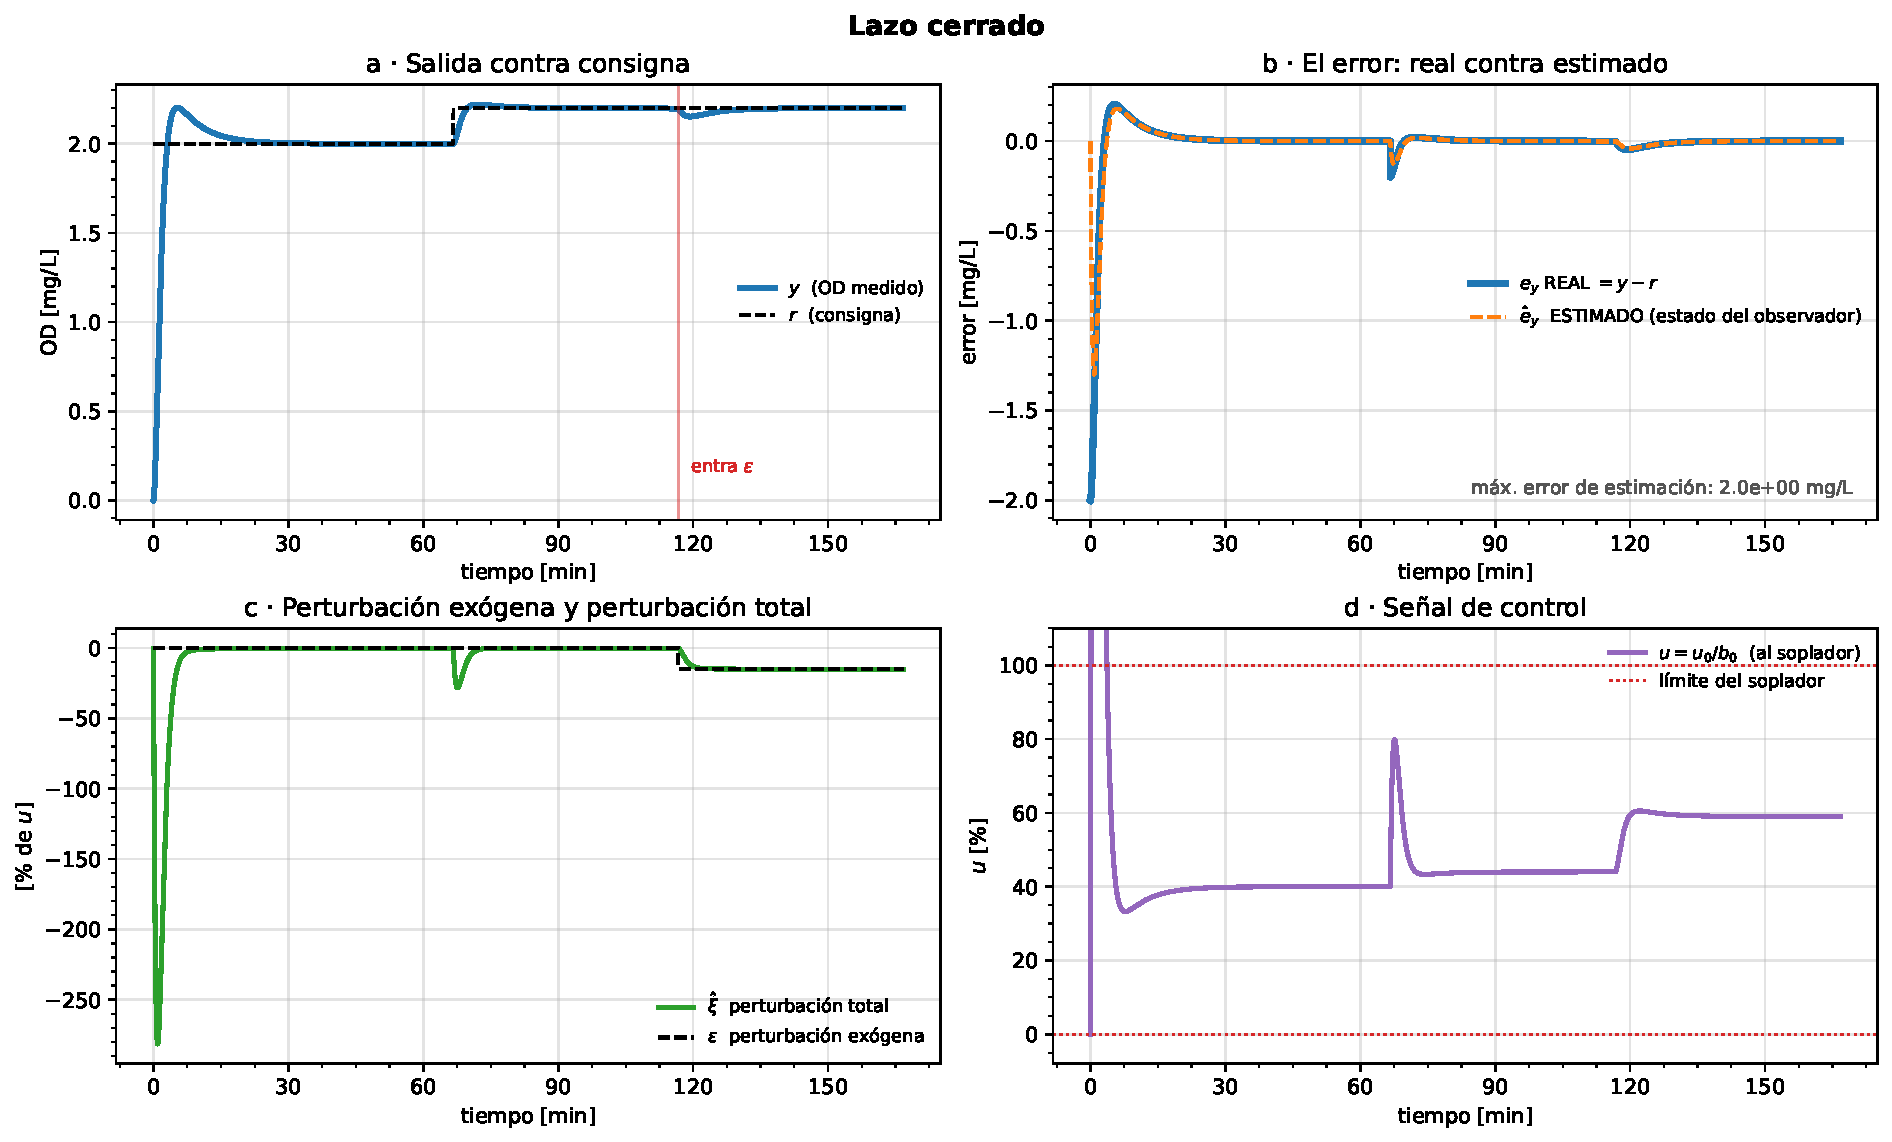
\includegraphics[width=\textwidth]{adrc_lazo_cerrado.pdf}
  \caption[Lazo cerrado usando ADRC basado en observador]{ (a) Salida contra consigna. (b) Error de seguimiento real y
    estimado. (c) Perturbación exógena y perturbación total. (d) Señal de control.}
  \label{fig:adrc_lazo_cerrado}
\end{figure}

El oxígeno disuelto sigue la consigna y rechaza la perturbación. En régimen estacionario, el
soplador queda en $40~\%$ a $2{,}0$~mg/L y en $44~\%$ a $2{,}2$~mg/L, que es lo
que cuesta sostener el OD; con la
perturbación sube a $59~\%$, y el observador también estima la entrada $\varepsilon$
($\hat{\xi}$ converge a $\varepsilon = -15~\%$). Ahora bien, el pico de control del
arranque, de unos $398~\%$, se debe a que se introduce el error de seguimiento en el observador y
el controlador debe compensar $u^* = \dot{y}^*$, y como $y^*$ es un escalón, su derivada es un delta
de Dirac, $\delta$, por lo que se va a ver reflejado también en su transitorio con un sobrepico.
Herbst y Madoński muestran esto en \cite[fig.~6.13]{herbst2024adrc}, donde lo llaman \emph{giant control
efforts}. Para evitarlo se suaviza la referencia: en el Capítulo~\ref{cap:implementacion} se usan un
polinomio de Bézier (Sección~\ref{subsec:impl_bezier}) y un prefiltro (Sección~\ref{sec:impl_esfuerzo}),
solo para los casos en los que entra un escalón, que es muy fuerte para este enfoque, y se mantienen las
propiedades del rechazo y del seguimiento.


%--------------------------------------------------------------------
\subsection{Márgenes de estabilidad y anchos de banda}
\label{subsec:caso_margenes}

La Figura~\ref{fig:adrc_frecuencia} muestra el lazo abierto
$G_L(s) = C(s)\,G(s)$, con $C(s)$ el ADRC visto desde $-e_y$ hasta $u$ (observador más ley de control), cuya función de transferencia se obtiene en la
Sección~\ref{sec:gpi_eso} \eqref{eq:gpi_eso_general}, y la planta
$G(s) = k_{dc}/(\tau s + 1)$. El margen de fase es de $65{,}8^{\circ}$ en
$\omega = 0{,}0104$~rad/s ($37{,}5$~rad/h), y el margen de ganancia es infinito,
porque la fase no cruza $-180^{\circ}$. El panel (c) muestra dónde quedan los
anchos de banda: la dinámica impuesta al error cae $3$~dB en $\omega_c$, y la
estimación de la perturbación, $\omega_o^2/(s+\omega_o)^2$, en $0{,}64\,\omega_o$.

\begin{figure}[H]
  \centering
  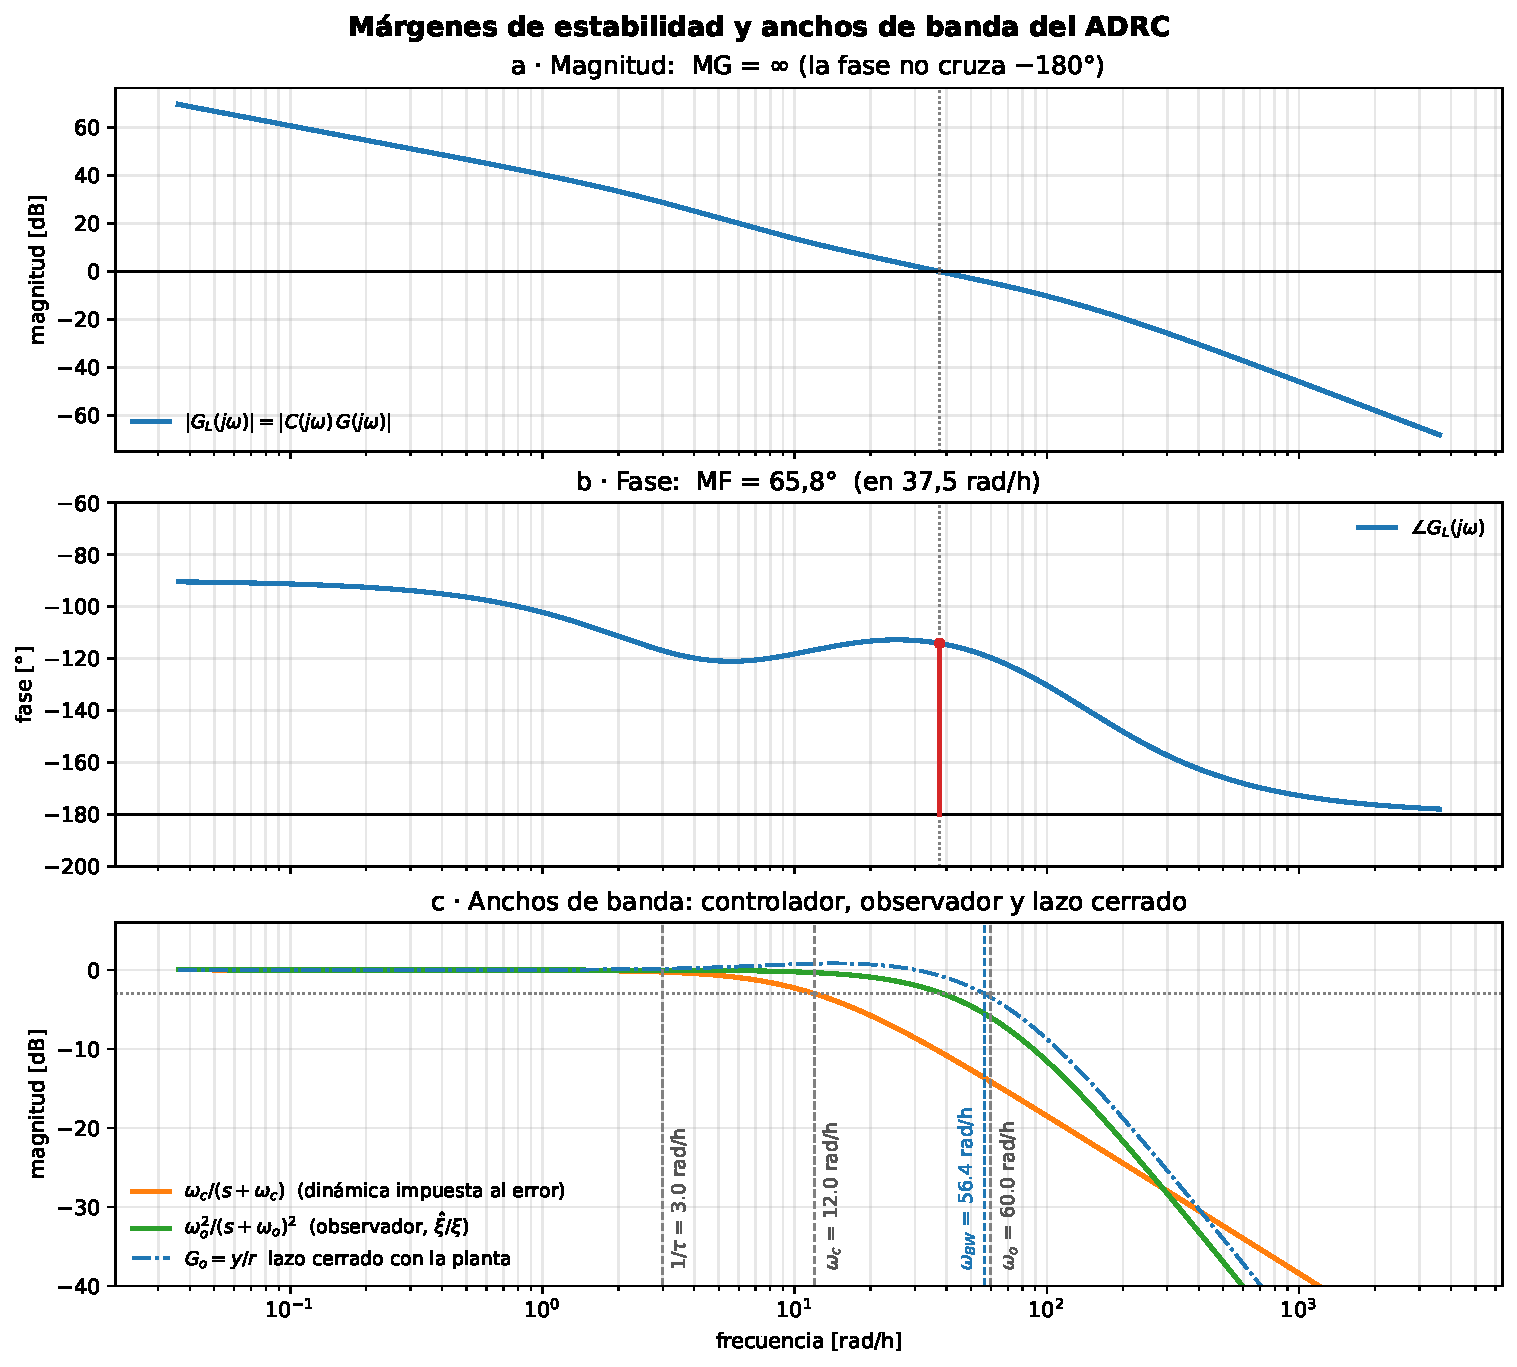
\includegraphics[width=0.85\textwidth]{adrc_frecuencia.pdf}
  \caption[Márgenes de estabilidad y anchos de banda del ADRC]{Márgenes de
    estabilidad y anchos de banda del ADRC con la planta. (a) Magnitud y
    (b) fase del lazo abierto $G_L(s) = C(s)\,G(s)$, con el cruce de ganancia y el
    margen de fase. (c) Magnitud de la dinámica impuesta al error, de la
    estimación de la perturbación en el observador y del lazo cerrado $y/r$, con
    $1/\tau$, $\omega_c$, $\omega_o$ y el ancho de banda del lazo cerrado,
    $\omega_{BW}$, marcados.}
  \label{fig:adrc_frecuencia}
\end{figure}

Con este margen la planta puede variar en fase
hasta $65{,}8^{\circ}$, por lo que sí tiene un grado de robustez, y aunque la planta tenga un retardo de
$50$~s el sistema puede seguir funcionando sin desestabilizarse: con $\theta = 50$~s el margen de fase baja a $36{,}0^{\circ}$ y
aparece un margen de ganancia de $2{,}12$ (Figura~\ref{fig:adrc_margenes_retardo}).

\begin{figure}[H]
  \centering
  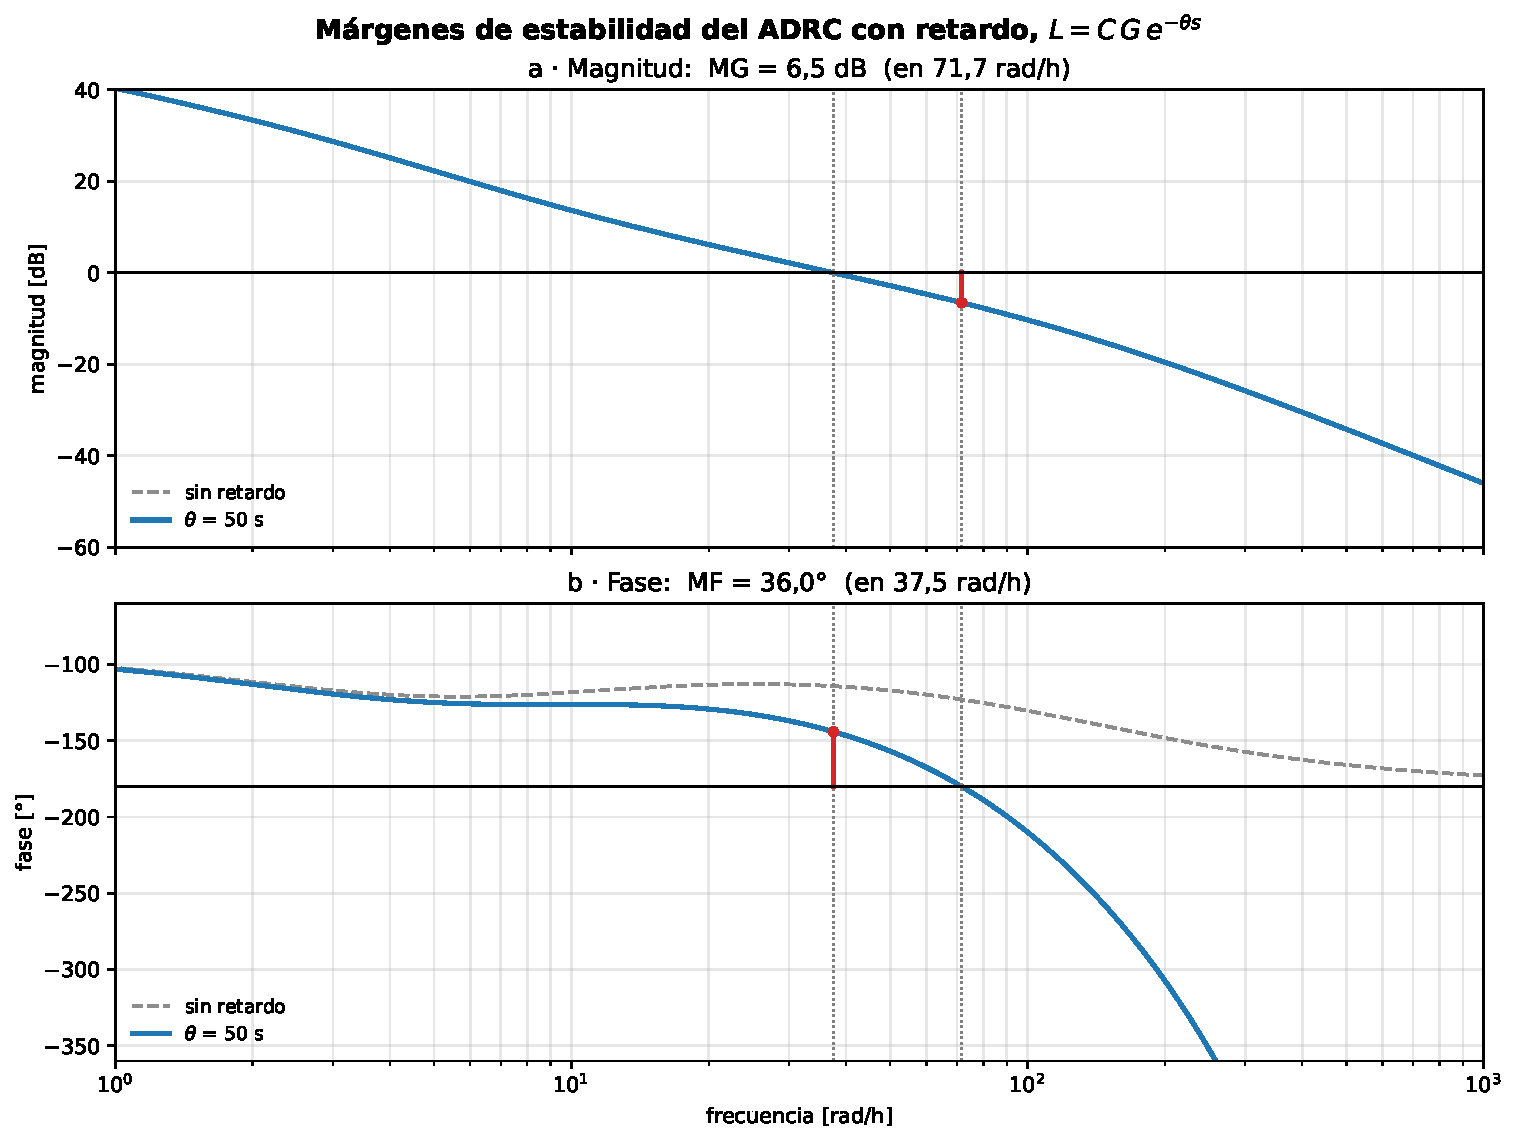
\includegraphics[width=0.85\textwidth]{adrc_margenes_retardo.pdf}
  \caption[Márgenes de estabilidad del ADRC con retardo]{Márgenes de
    estabilidad del lazo abierto con retardo, $G_{L_\theta}(s) = C(s)\,G(s)\,e^{-\theta s}$,
    con $\theta = 50$~s, frente al lazo sin retardo (gris). (a) Magnitud, con
    el margen de ganancia en el cruce de fase. (b) Fase, con el margen de fase
    en el cruce de ganancia.}
  \label{fig:adrc_margenes_retardo}
\end{figure}

%--------------------------------------------------------------------
\subsection{Variación de los parámetros de la planta}
\label{subsec:caso_variacion}

Para ver qué tanto depende el desempeño de la planta nominal, se repite el
escalón de consigna de $2{,}0$ a $2{,}2$~mg/L con el controlador fijo  y se varía un parámetro de
la planta a la vez (Figura~\ref{fig:adrc_variacion}). $K_{dc}$ y $\tau$ se toman
en los rangos intercuartílicos de los escalones de M2 y M3
(Sección~\ref{sec:ident_planta_diseno}): $K_{dc}$ entre $0{,}022$ y $0{,}109$~mg/(L$\cdot$\%) y
$\tau$ entre $11$ y $40$~min; con ellos cambia también el $b_0$ de la
planta, $b_{0,\mathrm{planta}} = k_{dc}/\tau$, entre $0{,}44$ y $2{,}18$ veces el de diseño. El retardo se
varía entre $0$ y $60$~s (Sección~\ref{sec:ident_retardo}). La referencia es
siempre la planta nominal ideal, sin retardo.

\begin{figure}[H]
  \centering
  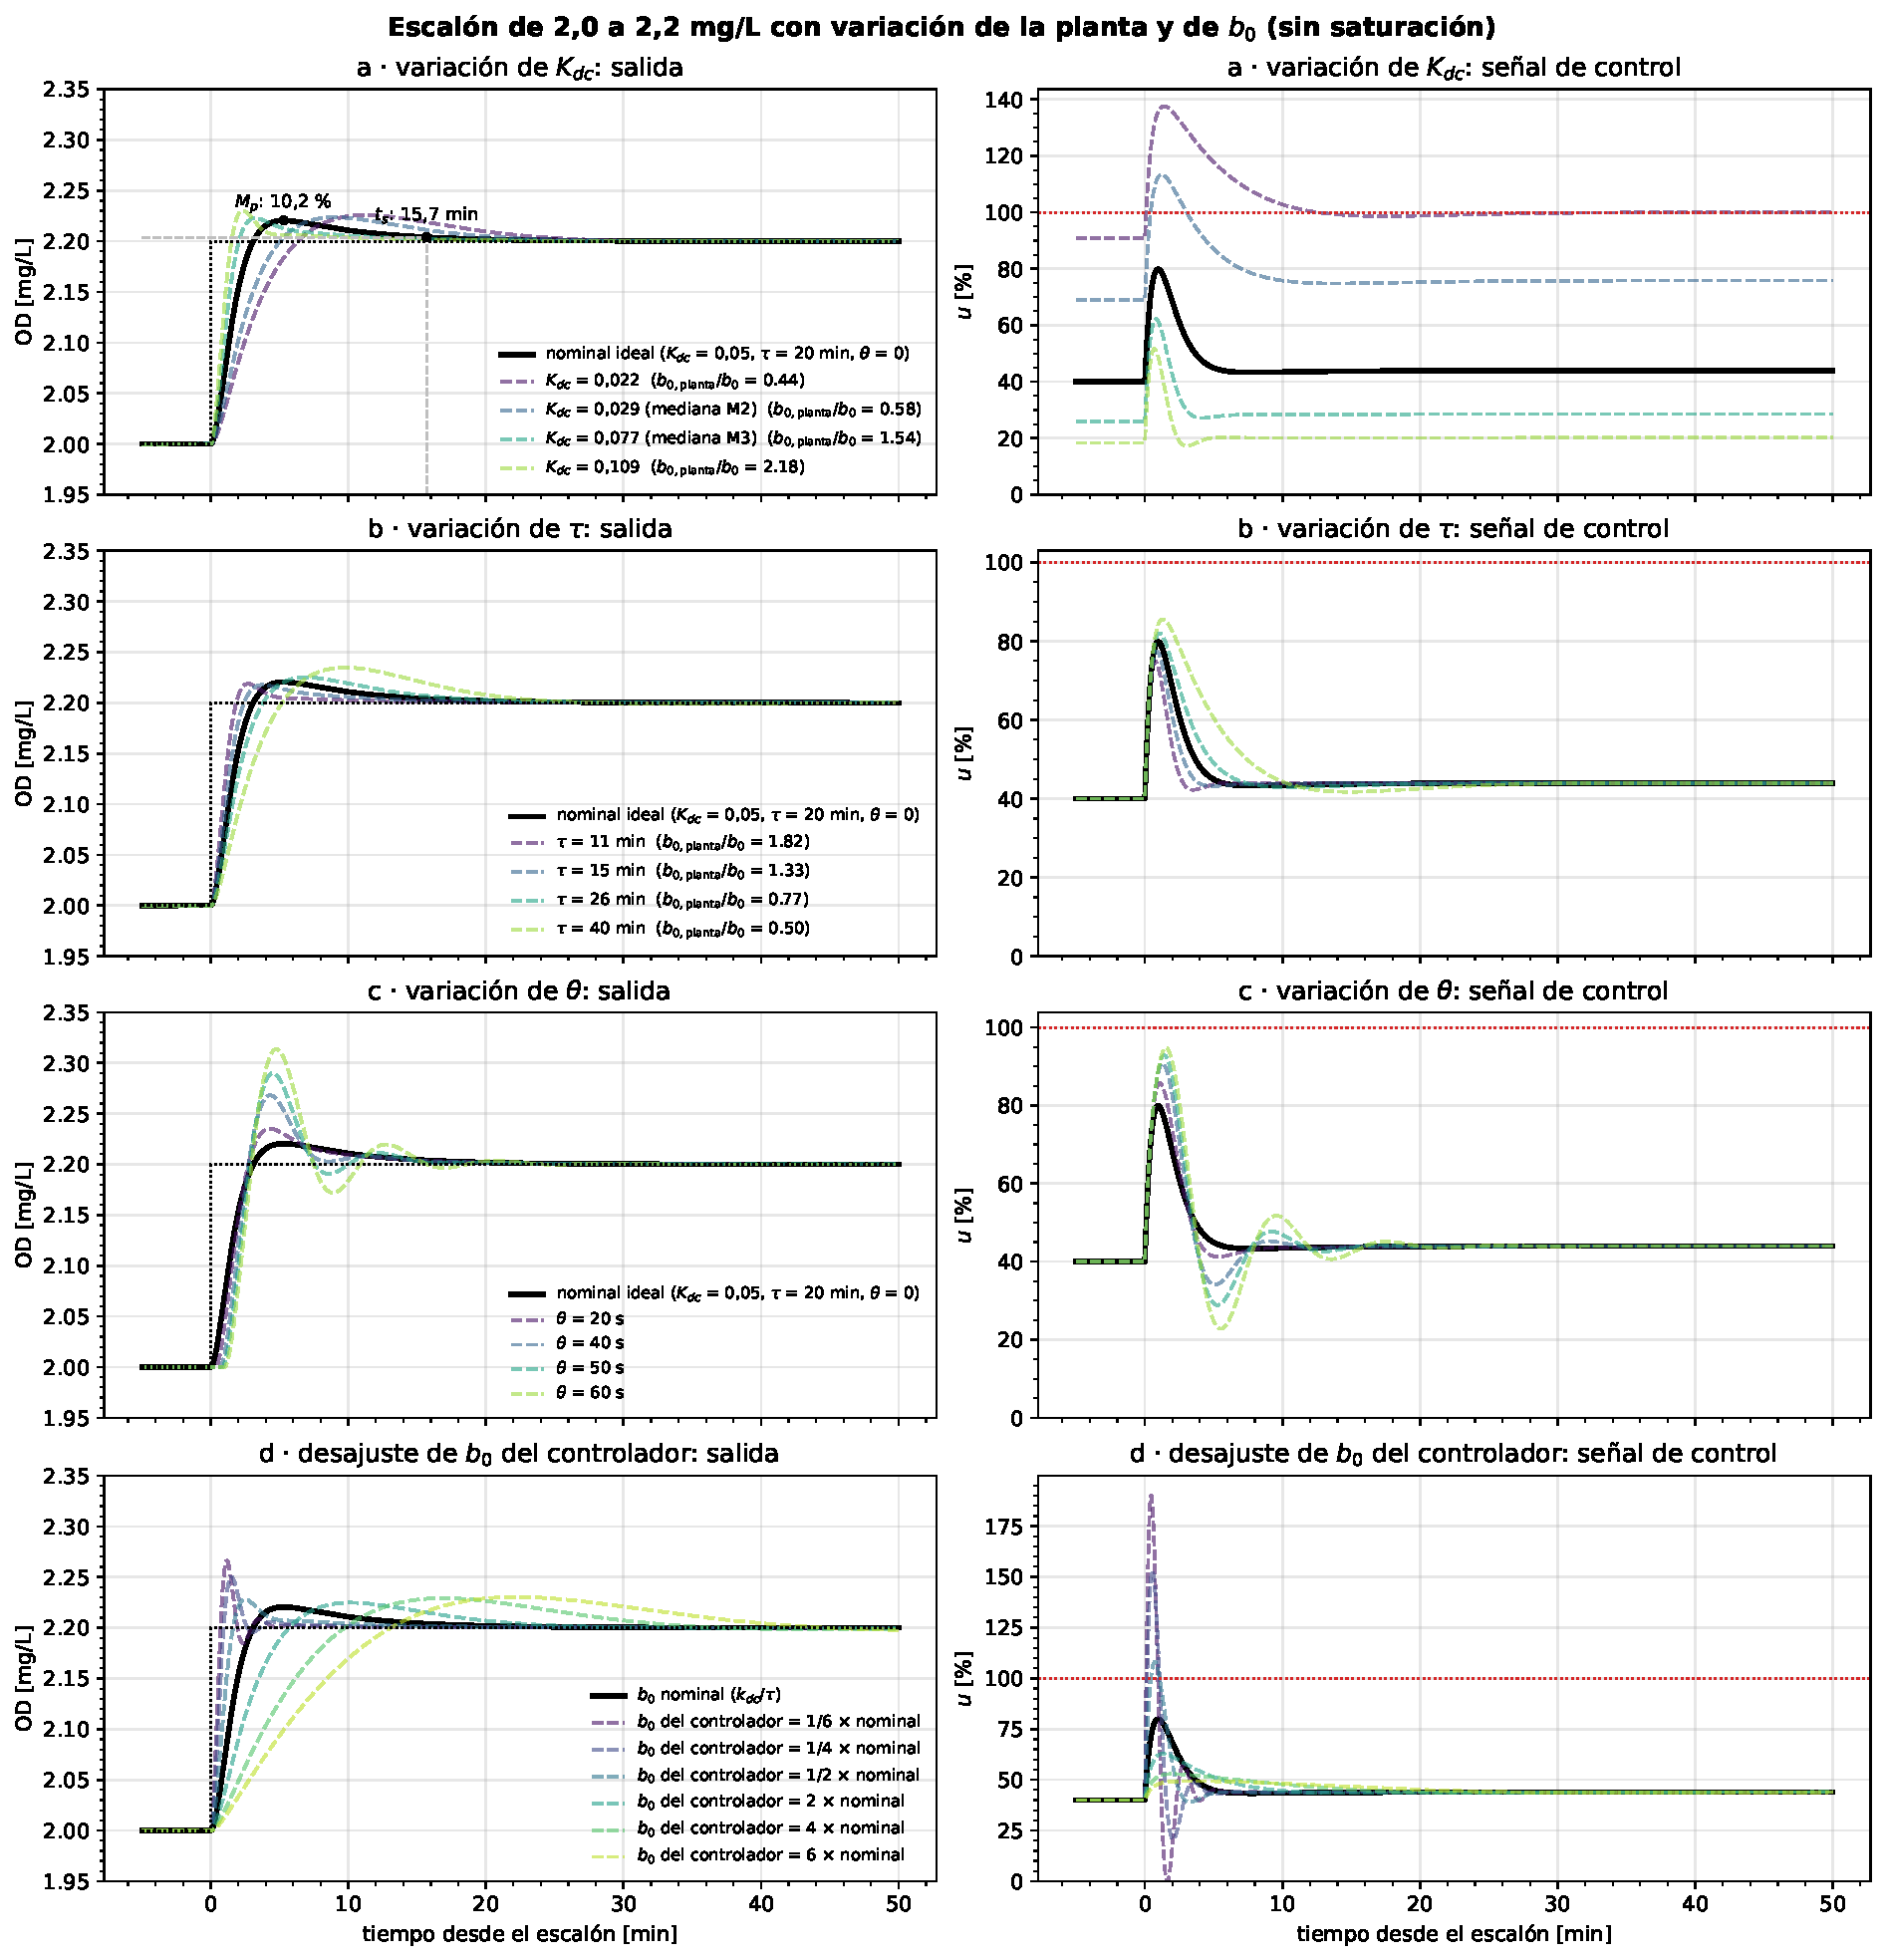
\includegraphics[width=\textwidth]{adrc_variacion_parametros.pdf}
  \caption[Escalón de consigna con variación de la planta y de $b_0$]{Escalón de consigna
    de $2{,}0$ a $2{,}2$~mg/L con el controlador nominal y variación de (a) la
    ganancia $K_{dc}$, (b) la constante de tiempo $\tau$ y (c) el retardo
    $\theta$ de la planta, y (d) desajuste del $b_0$ del controlador, sin
    saturación del actuador. En negro, la planta nominal ideal, con $M_p$ en
    \% del escalón y $t_s$ medido con banda de $2~\%$ del escalón, aproximadamente $4\cdot\tau$.}
  \label{fig:adrc_variacion}
\end{figure}

Con la $K_{dc}$ más alta, $0{,}109$, el OD se pasa un poco de la consigna, hasta
$2{,}23$~mg/L. Con la más baja, $0{,}022$, el controlador pide más esfuerzo: $u$
llega al $138~\%$, por encima de la saturación, y para sostener $2{,}2$~mg/L queda
justo en el $100~\%$; con una $K_{dc}$ menor, el soplador ya no alcanzaría para
llegar a la consigna (la Sección~\ref{subsec:sat_variacion} repite estos casos con saturación). La
constante de tiempo apenas cambia la respuesta; con $\tau$ más grande el
sobreimpulso crece un poco. El retardo es lo que más afecta: con $50$~s el pico
pasa de $2{,}22$ a $2{,}29$~mg/L, con una oscilación que se amortigua, coherente
con el margen de fase que deja el retardo (Sección~\ref{subsec:caso_margenes}).

El panel (d) repite el escalón con la planta nominal ideal y el $b_0$ del
controlador dividido y multiplicado por $2$, $4$ y $6$, sin cambiar los anchos de
banda. Lo que cuenta es la proporción entre el $b_0$ del controlador y el de la
planta: subestimarlo equivale a una planta con más ganancia, y sobreestimarlo, a
una con menos. Con $b_0$ subestimado el controlador es más agresivo (con $b_0/6$
el OD llega a $2{,}27$~mg/L y $u$ oscila con fuerza); con $b_0$ sobreestimado es
más suave, pero más lento (con $6\,b_0$ tarda unos $40$~min en asentarse, frente a
$16$~min del nominal). Para ver hasta dónde aguanta el lazo, se trazó el lugar de
las raíces variando solo esa proporción, $g = b_{0,\mathrm{planta}}/b_0$
(Figura~\ref{fig:adrc_rlocus_b0}): sin retardo el lazo es estable para cualquier
$g$, y con $\theta = 50$~s se vuelve inestable cuando $b_0$ queda por debajo de
$b_{0,\mathrm{planta}}/2{,}12$. Por eso conviene que, si hay duda, $b_0$ quede algo
por encima del de la planta: el lazo pierde velocidad, pero no robustez.

\begin{figure}[H]
  \centering
  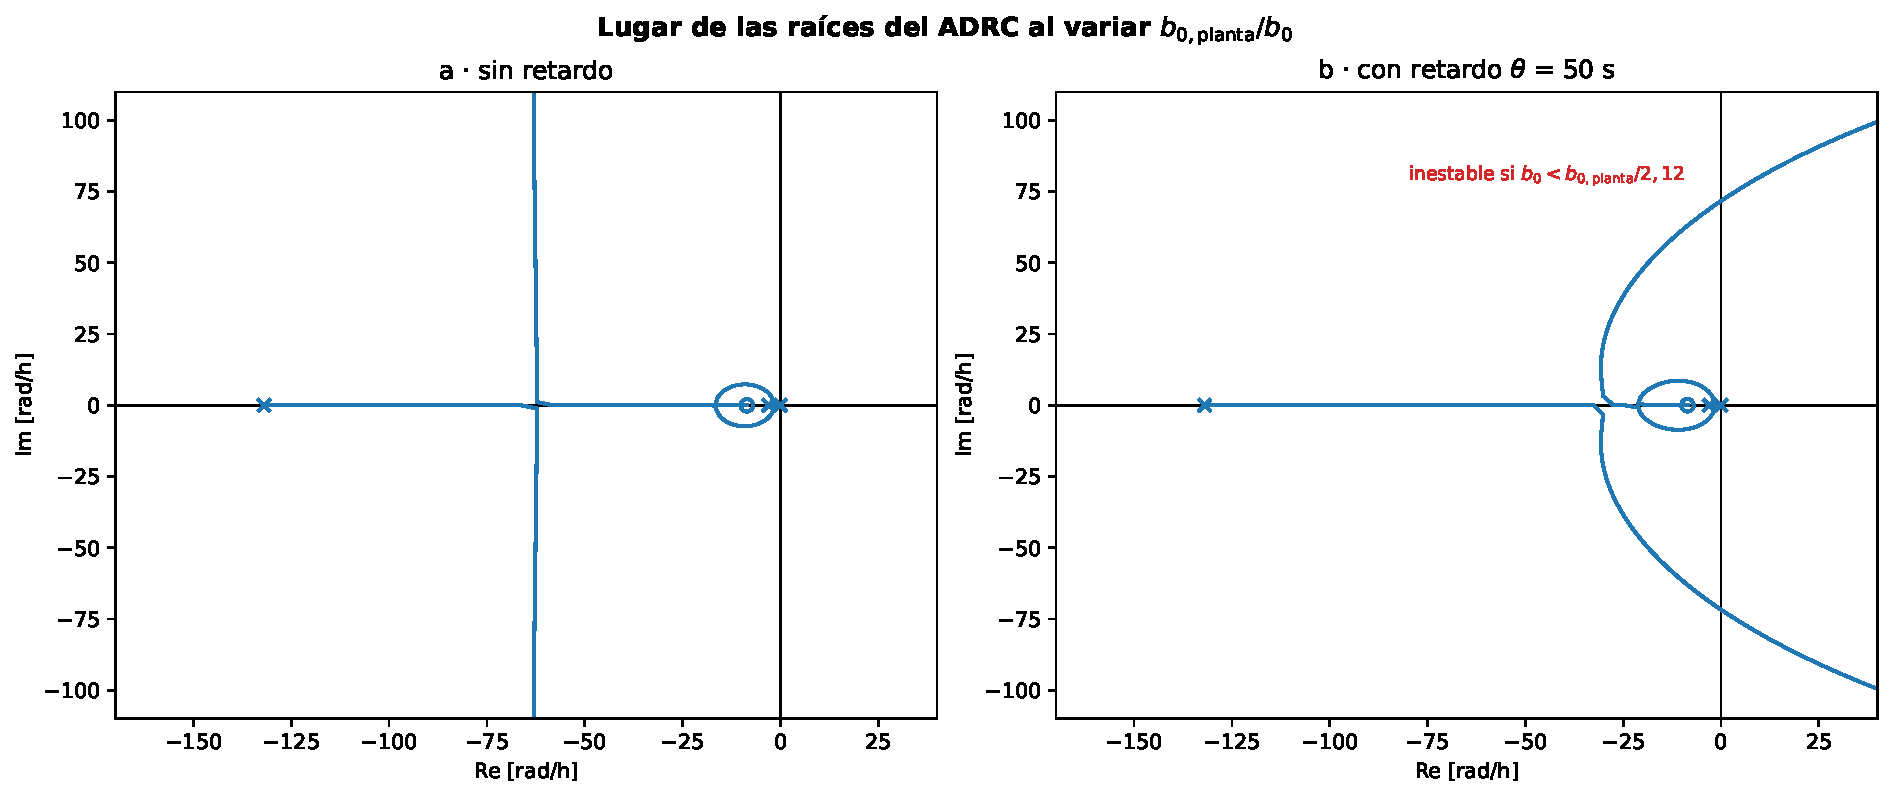
\includegraphics[width=\textwidth]{adrc_rlocus_b0.pdf}
  \caption[Lugar de las raíces del ADRC al variar el desajuste de $b_0$]{Lugar
    de las raíces del polinomio característico del lazo cerrado,
    $1 + g\,C(s)\,G(s) = 0$, al variar $g = b_{0,\mathrm{planta}}/b_0$, con $C(s)$
    la función de transferencia del ADRC con ESO \eqref{eq:mapa_C}, que se obtiene
    en la sección siguiente, y $G(s)$ la planta nominal: (a) sin retardo y (b) con
    $\theta = 50$~s (aproximación de Padé de orden 6). Las cruces son los polos de
    lazo abierto ($g = 0$) y los círculos, los ceros.}
  \label{fig:adrc_rlocus_b0}
\end{figure}

%--------------------------------------------------------------------
\subsection{Efecto de los anchos de banda}
\label{subsec:caso_mapas}

Para ver qué cambia en el lazo con la sintonía, los anchos de banda se varían
$\times 1/4$ a $4$ sobre el diseño de tres formas: $\omega_c$ con $\omega_o$
fijo, $\omega_o$ con $\omega_c$ fijo y los dos con $\omega_o/\omega_c = 5$,
siempre con la planta sin retardo y sin saturación. Para cada caso,
$k_p = \omega_c$, $l_1 = 2\omega_o$ y $l_2 = \omega_o^2$, y el ADRC visto de
$-e_y$ a $u$ es (Sección~\ref{subsec:gpi_eso_tf})
\begin{equation}
C(s) = \frac{1}{b_0}\,\frac{(k_p l_1 + l_2)\,s + k_p l_2}{s\,(s + k_p + l_1)} ,
\qquad
G_L(s) = C(s)\,G(s) ,
\qquad
G(s) = \frac{k_{dc}}{\tau s + 1} .
\label{eq:mapa_C}
\end{equation}
Primero se mira el escalón de consigna, luego las funciones de transferencia
del lazo y el margen de fase, y al final las Tablas~\ref{tab:adrc_iae_anchos}
y~\ref{tab:adrc_frecuencia_kESO} resumen los indicadores de cada caso.

\paragraph{Escalón de consigna.}
Se repite el escalón de $2{,}0$ a $2{,}2$~mg/L
(Figura~\ref{fig:adrc_pasos_anchos}). Con $y_{e}(t)$ la respuesta del
lazo cerrado $G_o(s) = G_L(s)/\bigl(1 + G_L(s)\bigr)$ al escalón unitario, $\Delta r = 0{,}2$~mg/L y
$t_f = 20\,000$~s, el error es $e(t) = \Delta r\,\bigl(1 - y_{e}(t)\bigr)$, y el sobrepico y el IAE se
calculan como en la Tabla~\ref{tab:metricas}.

\begin{figure}[H]
  \centering
  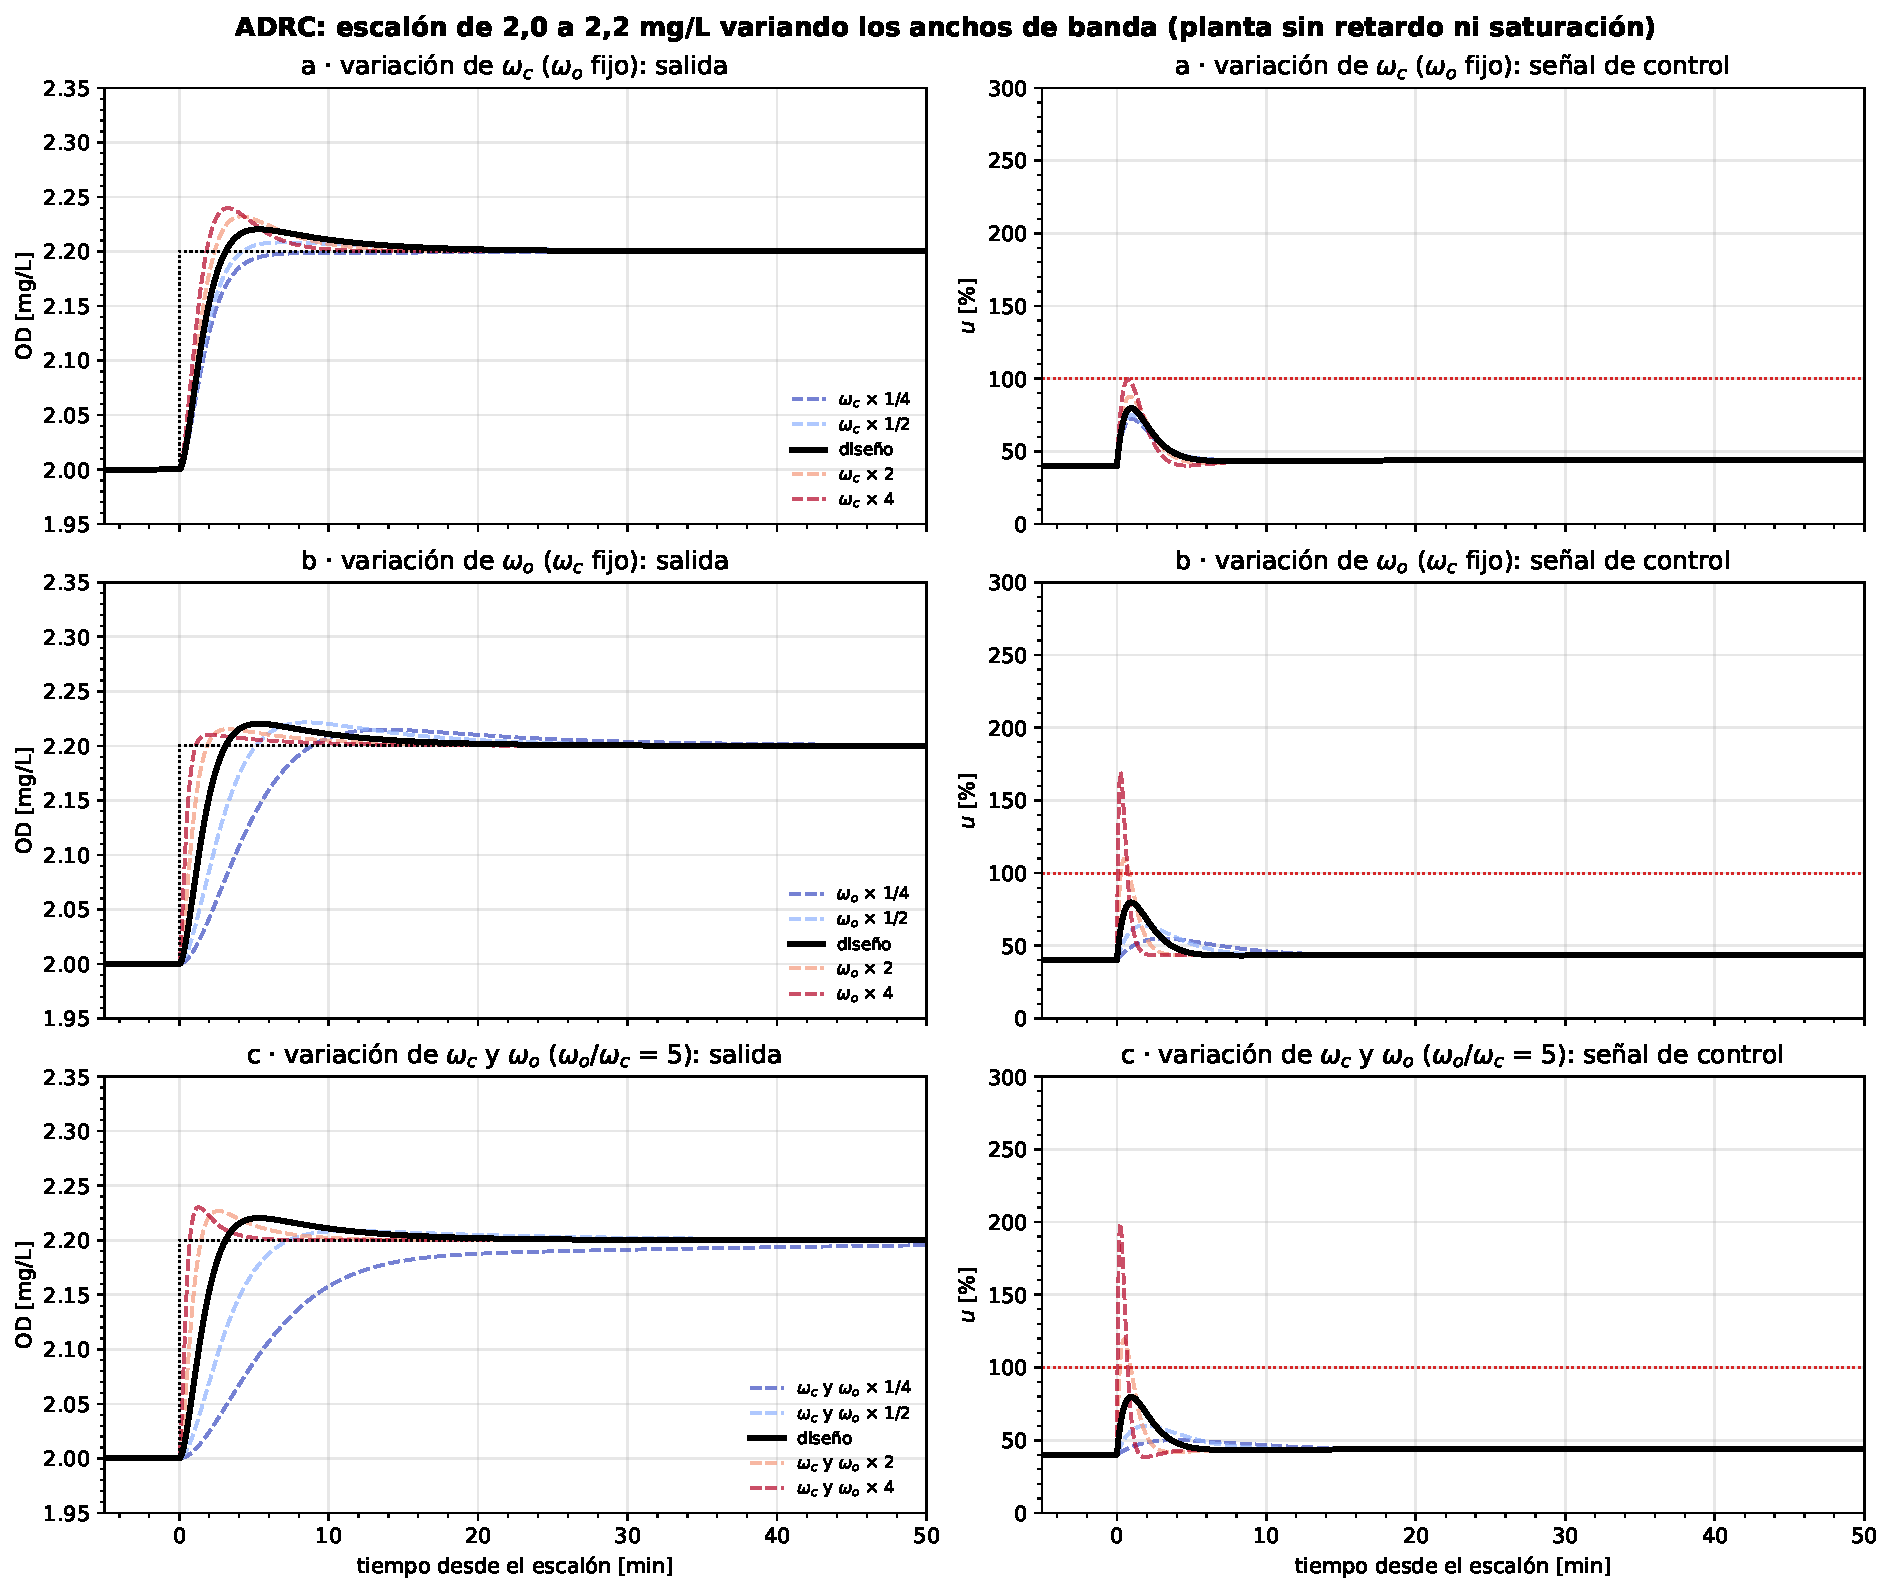
\includegraphics[width=\textwidth]{adrc_pasos_anchos.pdf}
  \caption[Escalón de consigna al variar los anchos de banda]{Escalón de
    consigna de $2{,}0$ a $2{,}2$~mg/L con la planta sin retardo ni
    saturación, variando (a) $\omega_c$ con $\omega_o$ fijo, (b) $\omega_o$ con
    $\omega_c$ fijo y (c) los dos con $\omega_o/\omega_c = 5$, por $1/4$, $1/2$,
    $2$ y $4$. Izquierda, la salida; derecha, la señal de control. En negro, el
    diseño de la Tabla~\ref{tab:caso_parametros}.}
  \label{fig:adrc_pasos_anchos}
\end{figure}

Al variar $\omega_c$ con $\omega_o$ fijo, se mueve
el sobrepico. Al incrementar $\omega_c$ se genera un mayor sobrepico, que
llega al $19{,}8~\%$ con $4\,\omega_c$, y el margen de fase baja
(Tabla~\ref{tab:adrc_frecuencia_kESO}). Al disminuirlo,
en cambio, se amplía la separación entre $\omega_c$ y $\omega_o$, y la respuesta
transitoria es más suave y con mayor margen de fase: con $\omega_c/4$ ya no hay
sobrepico y el margen sube de $65{,}8^{\circ}$ a $76{,}3^{\circ}$.

Lo contrario pasa al variar $\omega_o$ con $\omega_c$ fijo. Al subir $\omega_o$
el sistema se comporta más rápido (con $4\,\omega_o$ se asienta en $7$~min y el
IAE baja de $26{,}9$ a $8{,}8$~mg$\cdot$s/L), pero esa rapidez se debe al
sobreesfuerzo de la señal de control, que llega al $169~\%$. En el esquema
basado en el error, el escalón de consigna entra en $\xi$ como la derivada de la
referencia, $u^* = \dot{y}^*$ (Sección~\ref{subsec:caso_simulacion}), y entre
más alto es $\omega_o$, más rápido la estima el observador y con más fuerza la
compensa el controlador. Esto se puede mejorar ajustando $\omega_o$: al
disminuirlo, el rechazo no es tan fuerte y la señal de control no crece tanto
($64~\%$ con $\omega_o/2$), aunque la respuesta se vuelve más lenta. De esta
manera, con $\omega_o$ se puede manipular un poco la velocidad del transitorio
del sistema.

\paragraph{Funciones de transferencia del lazo.}
\label{subsec:caso_gang}
Con la perturbación de entrada $\varepsilon$ y el ruido $n$ a la salida
(Figura~\ref{fig:caso_lazo_gang}), las funciones de transferencia del lazo son
las de la Tabla~\ref{tab:caso_gang}, con $G(s)$ y $C(s)$ de \eqref{eq:mapa_C}.
En esta figura, $y$ es la medida, con el ruido incluido.

\begin{figure}[H]
  \centering
  \begin{tikzpicture}[every path/.style={thick}]
    \node[sum] (s1) at (1.2,0) {};
    \node[block, minimum width=1.6cm] (c) at (3.6,0) {$C(s)$};
    \node[sum] (s2) at (5.8,0) {};
    \node[block, minimum width=1.6cm] (g) at (7.8,0) {$G(s)$};
    \node[sum] (s3) at (9.9,0) {};
    \coordinate (yb) at (10.9,0);
    \draw[->] (-0.3,0) node[above right] {$r(t)$} -- (s1.west);
    \node[sgn] at ($(s1.west)+(-0.15,0.25)$) {$+$};
    \draw[->] (s1.east) -- node[above] {$-e_y(t)$} (c.west);
    \draw[->] (c.east) -- node[above] {$u(t)$} (s2.west);
    \draw[->] (s2 |- 0,1.2) node[above] {$\varepsilon(t)$} -- (s2.north);
    \draw[->] (s2.east) -- (g.west);
    \draw[->] (s3 |- 0,1.2) node[above] {$n(t)$} -- (s3.north);
    \draw[->] (g.east) -- (s3.west);
    \draw (s3.east) -- (yb);
    \draw[->] (yb) -- (11.9,0) node[above left] {$y(t)$};
    \fill (yb) circle (1.5pt);
    \draw[->] (yb) -- (10.9,-1.2) -- (1.2,-1.2) -- (s1.south);
    \node[sgn] at ($(s1.south)+(-0.25,-0.15)$) {$-$};
  \end{tikzpicture}
  \caption[Lazo con perturbación de entrada y ruido]{Lazo con la perturbación
    de entrada $\varepsilon$ (en \% de $u$) y el ruido $n$ a la salida; $y$ es
    la medida.}
  \label{fig:caso_lazo_gang}
\end{figure}

\begin{table}[H]
\centering
\caption[Funciones de transferencia del lazo]{Funciones de transferencia del
  lazo de la Figura~\ref{fig:caso_lazo_gang}.}
\label{tab:caso_gang}
\renewcommand{\arraystretch}{2.2}
\begin{tabular}{lccc}
\toprule
\textbf{Entrada / salida} & $-e_y = r - y$ & $u$ & $y$ \\
\midrule
$r$           & $\dfrac{1}{1 + CG}$  & $\dfrac{C}{1 + CG}$   & $\dfrac{CG}{1 + CG}$ \\
$\varepsilon$ & $\dfrac{-G}{1 + CG}$ & $\dfrac{-CG}{1 + CG}$ & $\dfrac{G}{1 + CG}$  \\
$n$           & $\dfrac{-1}{1 + CG}$ & $\dfrac{-C}{1 + CG}$  & $\dfrac{1}{1 + CG}$  \\
\bottomrule
\end{tabular}
\end{table}

\begin{figure}[H]
  \centering
  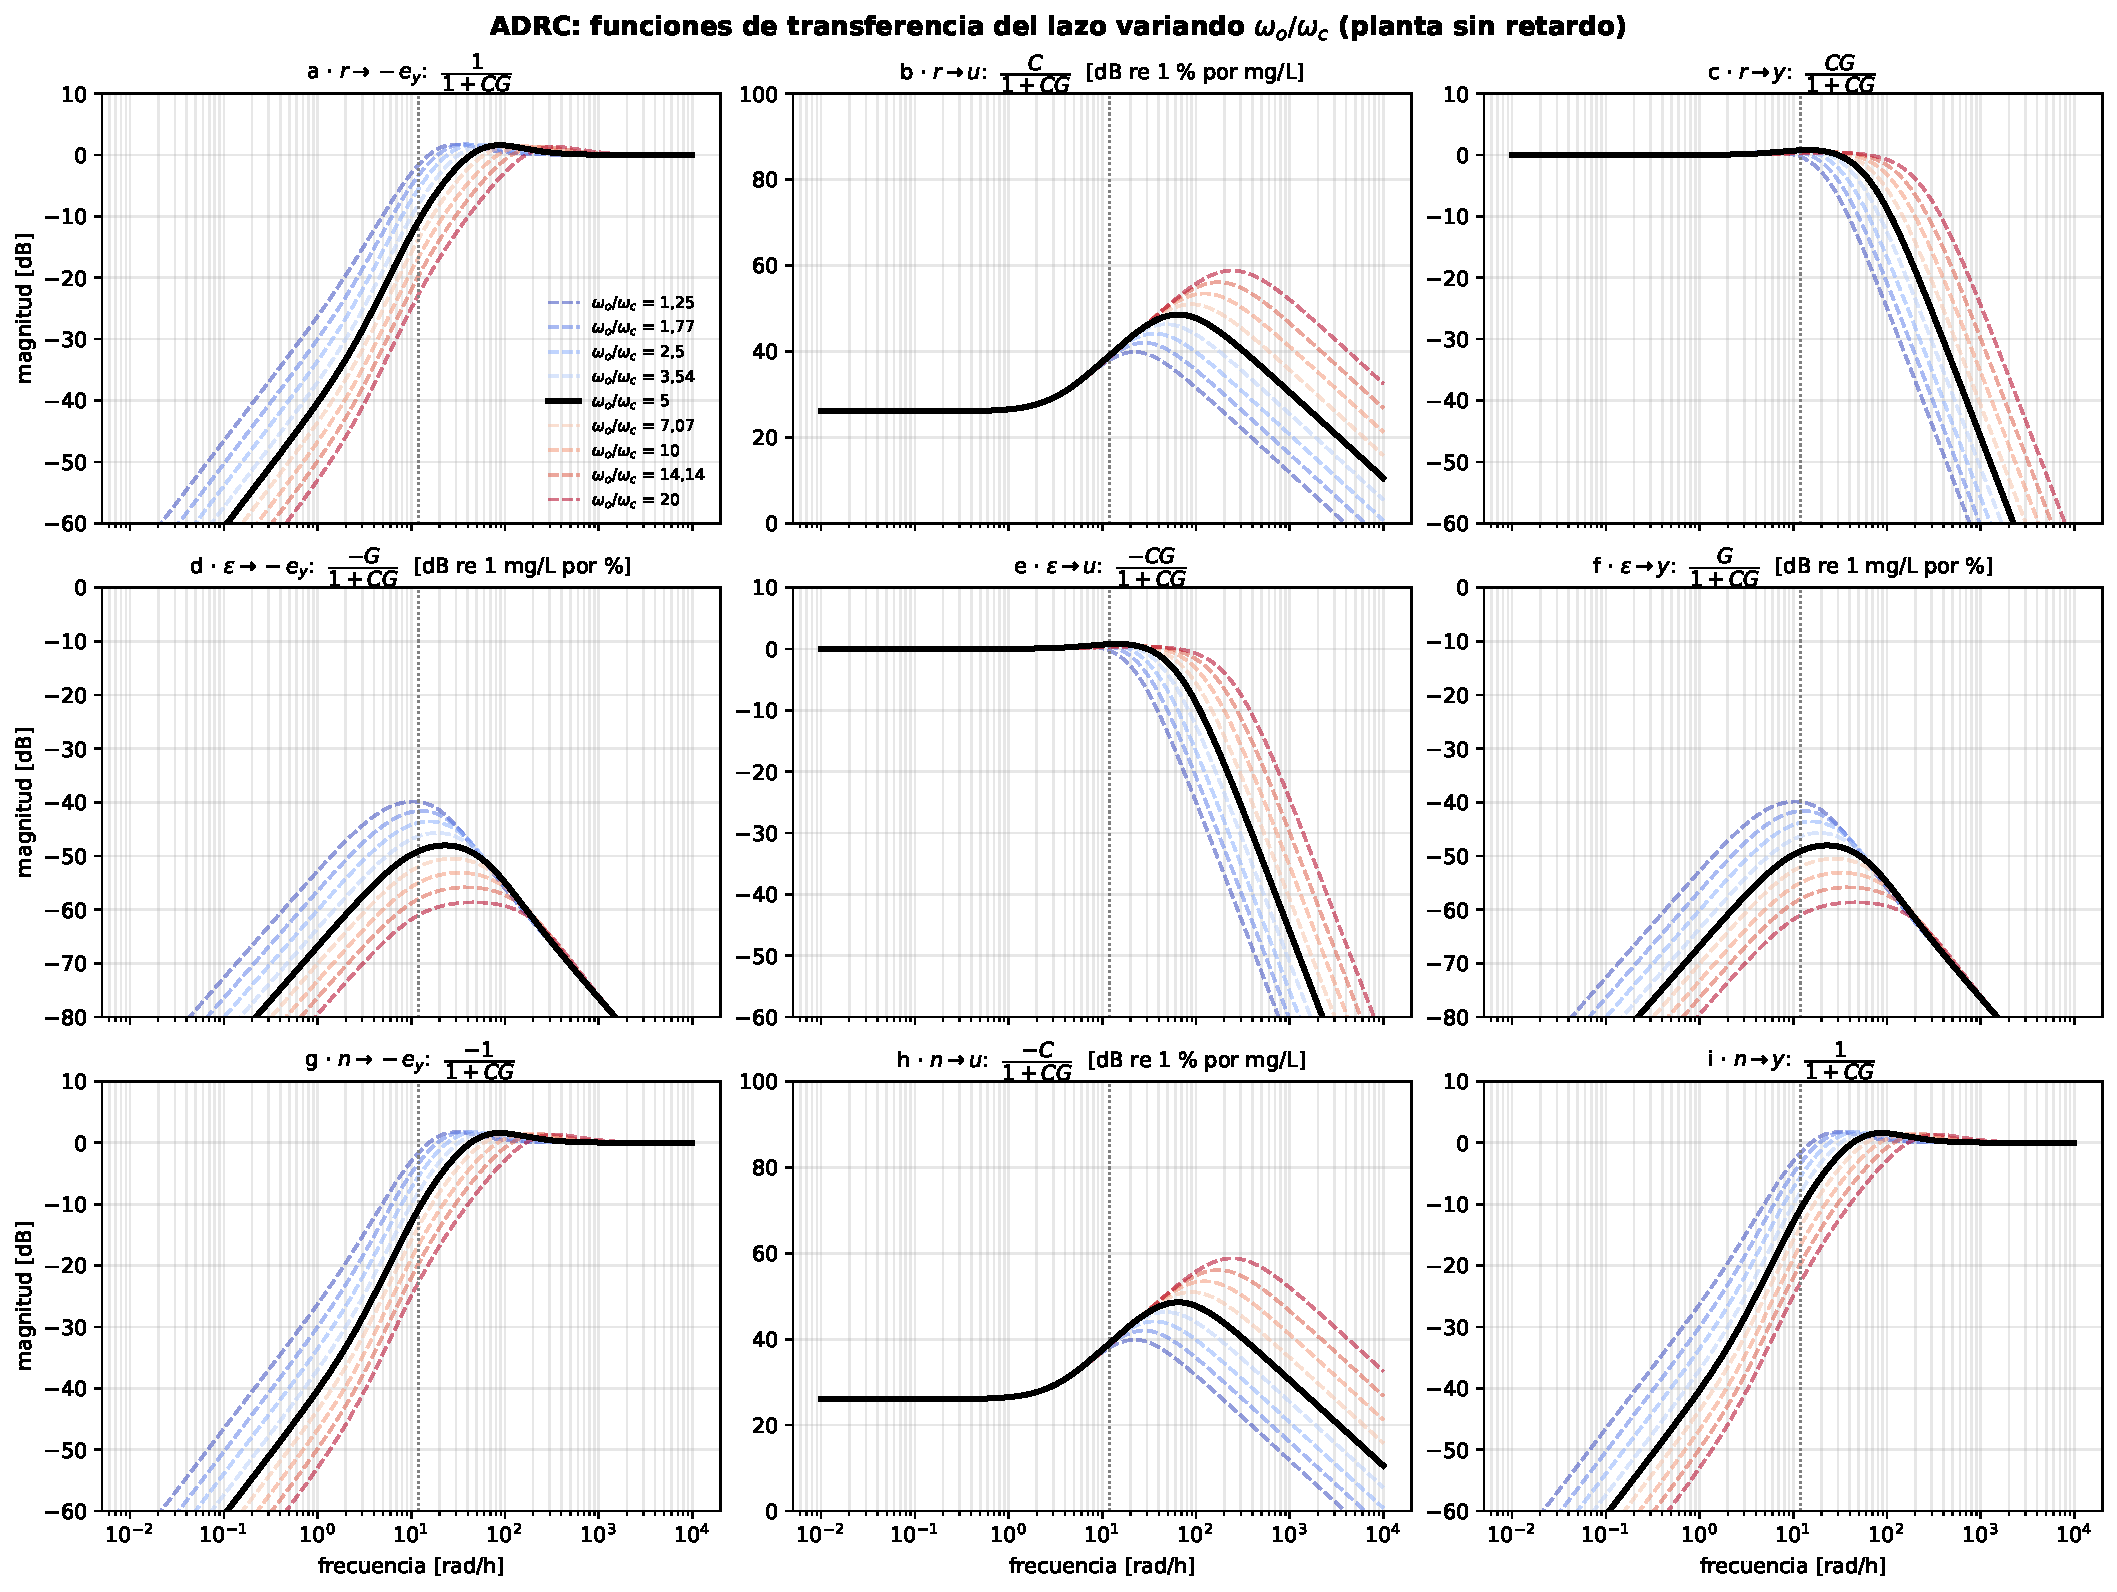
\includegraphics[width=\textwidth]{adrc_gang_kESO.pdf}
  \caption[Funciones de transferencia del lazo al variar
    $\omega_o/\omega_c$]{Funciones de transferencia de la
    Tabla~\ref{tab:caso_gang} con la planta sin retardo, $\omega_c$ fijo y
    $\omega_o/\omega_c$ de $1{,}25$ a $20$ (en negro, el diseño,
    $\omega_o = 5\,\omega_c$). Por filas, de $r$, $\varepsilon$ y $n$; por
    columnas, hacia $-e_y$, $u$ e $y$. La vertical marca $\omega_c$.}
  \label{fig:adrc_gang_kESO}
\end{figure}

La Figura~\ref{fig:adrc_gang_kESO} muestra cómo cambian al subir
$\omega_o/\omega_c$ con $\omega_c$ fijo. Aunque son nueve, en magnitud solo hay
cuatro curvas distintas, porque el signo no cambia la magnitud (por eso da lo
mismo mirar $e_y$ o $-e_y$): $1/(1 + CG)$ en (a), (g) e (i); $CG/(1 + CG)$ en (c)
y (e); $G/(1 + CG)$ en (d) y (f), y $C/(1 + CG)$ en (b) y (h). Con ellas se ve
qué sigue el lazo, qué rechaza y qué filtra:
\begin{itemize}
  \item \textbf{Seguimiento} (a y c). Al subir $\omega_o/\omega_c$, la salida
  sigue la consigna hasta frecuencias más altas y el error se corrige antes.
  \item \textbf{Rechazo de la perturbación} (d, e y f). El pico de la función de transferencia
  $y/\varepsilon$ baja al subir $\omega_o/\omega_c$, o sea que la
  perturbación se rechaza mejor, y en (e) se ve que $u$ la compensa hasta
  frecuencias más altas; es decir, el rechazo mejora cuando aumenta $\wo$.
  \item \textbf{Esfuerzo de control y ruido} (b y h). La ganancia de $C(s)$ sube con
  $\omega_o/\omega_c$ (Figura~\ref{fig:adrc_C_kESO}). Por eso un $\omega_o$ alto
  pide más señal de control ante el escalón y deja pasar más ruido del sensor
  al soplador, por lo que se deben ajustar bien las ganancias para que el ruido no llegue a la
  señal de control.
\end{itemize}
Es decir, con la relación $\omega_o/\omega_c$ se escoge qué tan rápido se sigue
la consigna y se rechaza la perturbación, a cambio de cuánto ruido se filtra.

\begin{figure}[H]
  \centering
  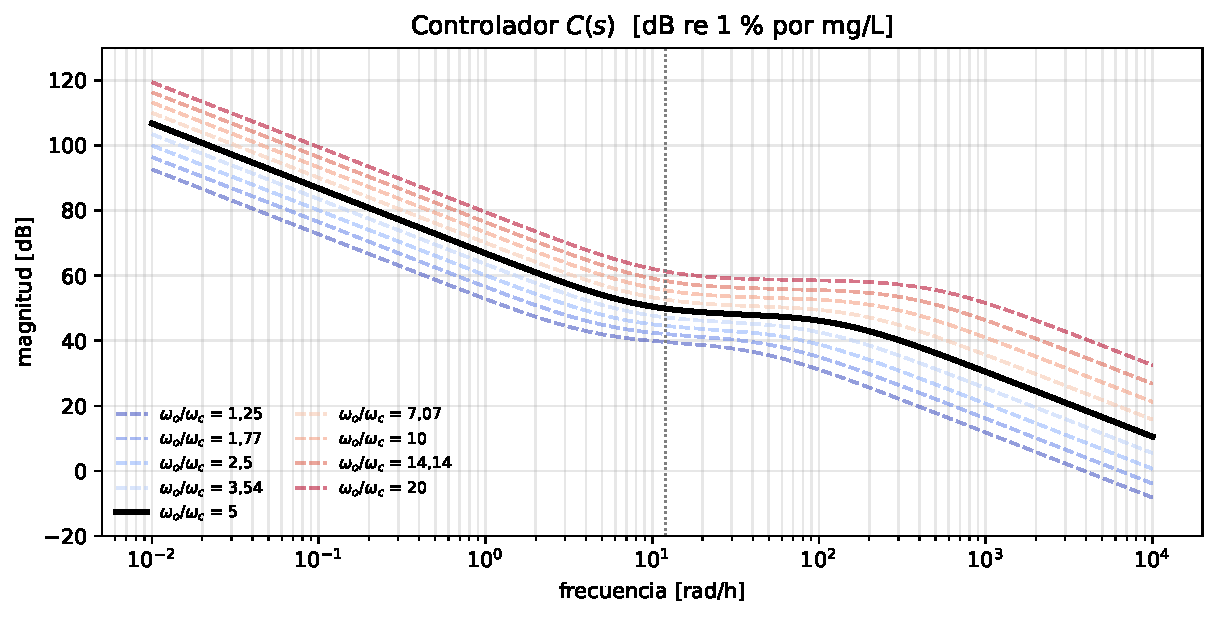
\includegraphics[width=0.8\textwidth]{adrc_C_kESO.pdf}
  \caption[Controlador del ADRC al variar $\omega_o/\omega_c$]{Magnitud del
    controlador $C(s)$ \eqref{eq:mapa_C} con $\omega_c$ fijo y
    $\omega_o/\omega_c$ de $1{,}25$ a $20$ (en negro, el diseño). La vertical
    marca $\omega_c$.}
  \label{fig:adrc_C_kESO}
\end{figure}

\paragraph{Margen de fase.}
La robustez se mide con el margen de fase, el retardo máximo que aguanta el
lazo y la sensibilidad máxima,
\begin{equation}
\begin{gathered}
\mathrm{MF} = 180^{\circ} + \angle G_L(j\omega_{gc}),\quad |G_L(j\omega_{gc})| = 1 ,
\qquad
\theta_{\max} = \frac{\pi}{180^{\circ}}\,\frac{\mathrm{MF}}{\omega_{gc}} ,\\[4pt]
M_s = \max_{\omega}\,|S(j\omega)|,\quad S(s) = \frac{1}{1 + G_L(s)} .
\end{gathered}
\label{eq:mapa_robustez}
\end{equation}
La Figura~\ref{fig:adrc_margen_fase_kESO} compara dos formas de cambiar la
relación $\omega_o/\omega_c$: moviendo $\omega_o$ con $\omega_c$ fijo
(izquierda) o moviendo $\omega_c$ con $\omega_o$ fijo (derecha). Al subir la
relación por encima del diseño se obtiene más fase, pero para una misma
relación da mejor resultado bajar $\omega_c$ que subir $\omega_o$: se gana más
margen y el cruce de ganancia baja un poco, así que el lazo también aguanta más
retardo. Al subir
$\omega_o$, en cambio, el cruce se va a frecuencias más altas y el retardo que
aguanta el lazo baja, hasta quedar por debajo de los $50$~s de diseño con
$\omega_o/\omega_c \approx 14$. Por eso, si se busca más margen, conviene bajar
$\omega_c$ antes que subir $\omega_o$.

\begin{figure}[H]
  \centering
  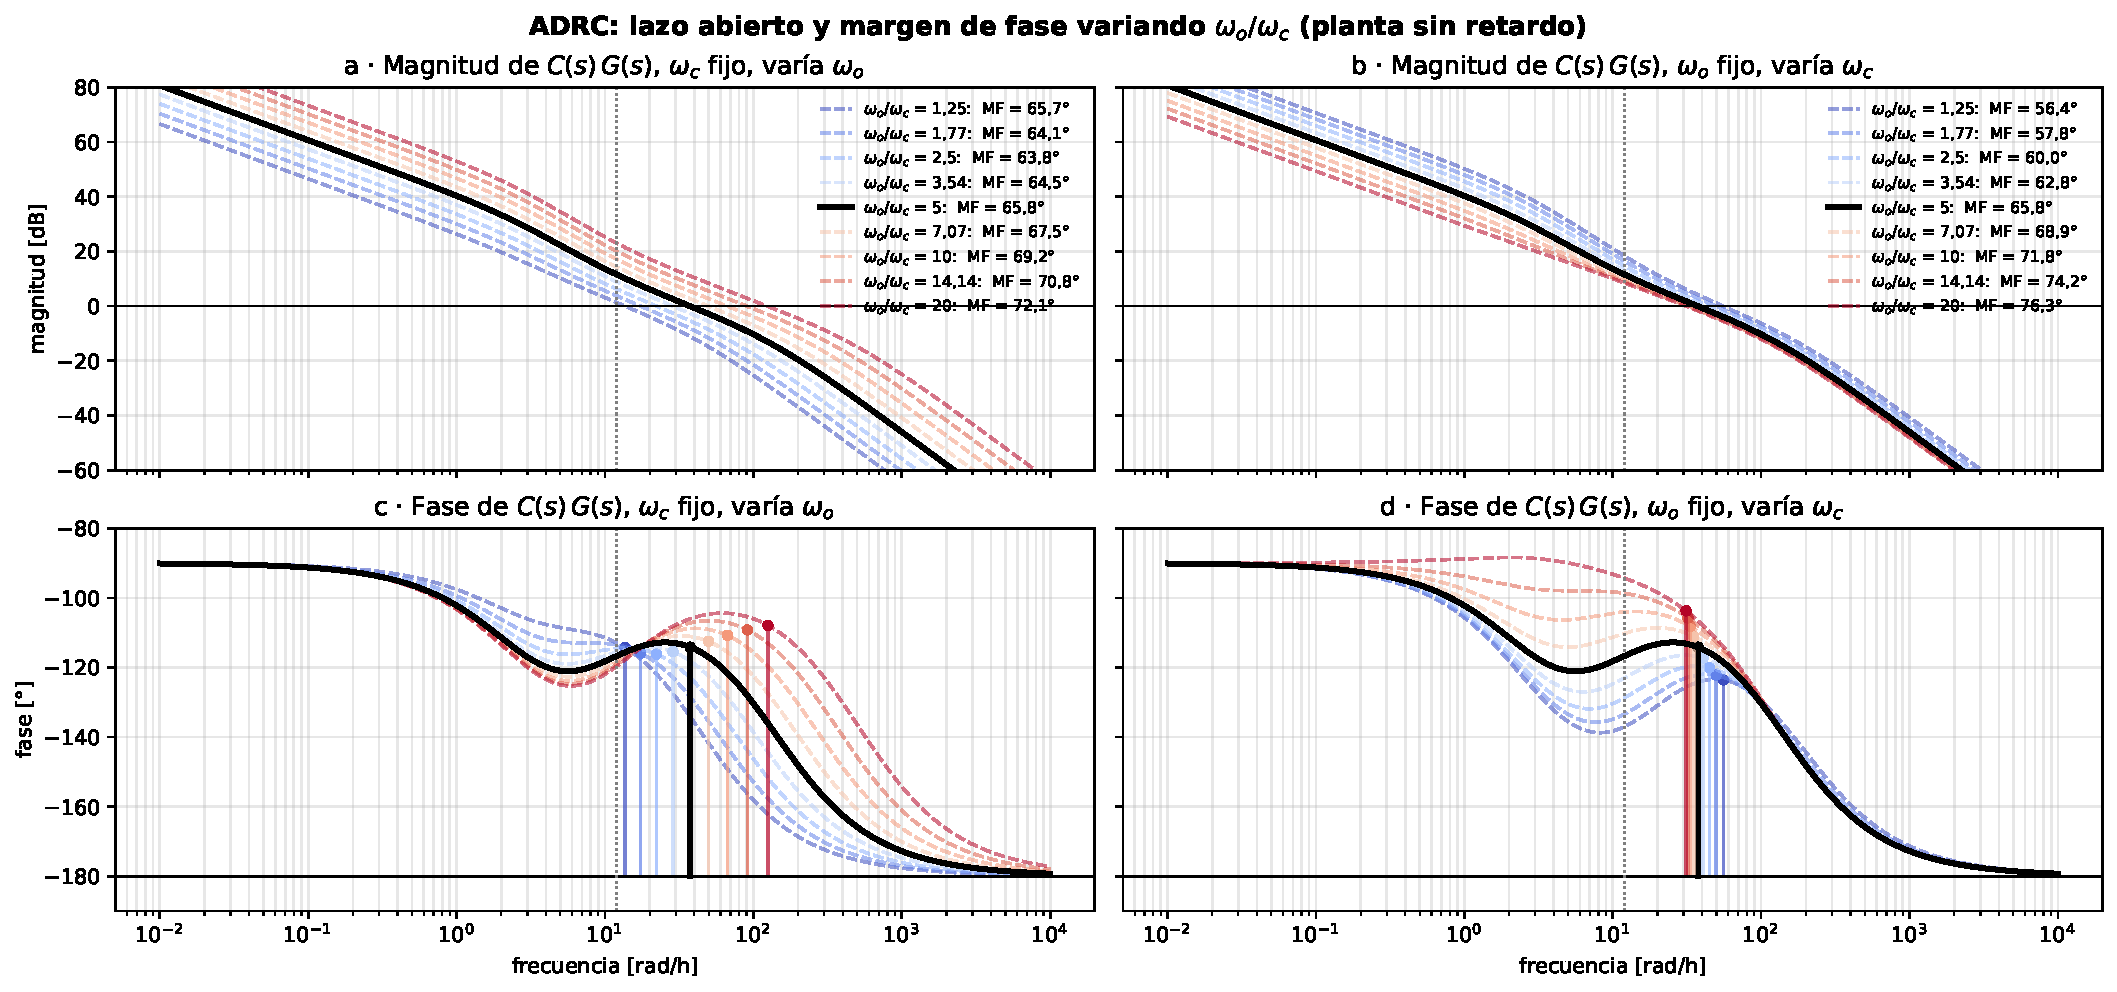
\includegraphics[width=\textwidth]{adrc_margen_fase_kESO.pdf}
  \caption[Margen de fase al variar $\omega_o/\omega_c$]{Lazo abierto
    $C(s)\,G(s)$ con la planta sin retardo y $\omega_o/\omega_c$ de $1{,}25$ a
    $20$ (en negro, el diseño): (a) y (c) con $\omega_c$ fijo, variando
    $\omega_o$; (b) y (d) con $\omega_o$ fijo, variando $\omega_c$. Arriba, la
    magnitud; abajo, la fase, con el margen de fase \eqref{eq:mapa_robustez}
    como segmento vertical y su valor en la leyenda.}
  \label{fig:adrc_margen_fase_kESO}
\end{figure}

\paragraph{Resumen.}
Las Tablas~\ref{tab:adrc_iae_anchos} y~\ref{tab:adrc_frecuencia_kESO} resumen
los tres barridos, la primera en el tiempo y la segunda en frecuencia. En
pocas palabras, $\omega_c$ define la forma de la respuesta y el margen de fase,
y $\omega_o$ define la velocidad, el rechazo de la perturbación y cuánto ruido
llega al soplador. Subir $\omega_o$ mejora el seguimiento y el rechazo, pero
pide más señal de control, deja pasar más ruido y aguanta menos retardo; bajar
$\omega_c$ suaviza la respuesta y da más margen sin pedir más esfuerzo.

\begin{table}[H]
\centering
\caption[Desempeño del escalón al variar los anchos de banda]{Escalón de
  $2{,}0$ a $2{,}2$~mg/L de la Figura~\ref{fig:adrc_pasos_anchos}: sobrepico $M_p$, tiempo de
  asentamiento $t_s$, IAE y pico de la señal de control (Tabla~\ref{tab:metricas}).}
\label{tab:adrc_iae_anchos}
\small
\begin{tabular}{llrrrr}
\toprule
\textbf{Variación} & \textbf{Factor} & $M_p$ [\%] & $t_s$ [min] & IAE [mg$\cdot$s/L] & $u_{\max}$ [\%] \\
\midrule
diseño & $1$ & $10{,}2$ & $15{,}7$ & $26{,}9$ & $80$ \\
\midrule
$\omega_c$ ($\omega_o$ fijo) & $1/4$ & $0{,}0$ & $5{,}7$ & $24{,}6$ & $72$ \\
 & $1/2$ & $4{,}1$ & $16{,}0$ & $26{,}6$ & $75$ \\
 & $2$ & $16{,}1$ & $11{,}7$ & $24{,}1$ & $88$ \\
 & $4$ & $19{,}8$ & $8{,}7$ & $20{,}1$ & $100$ \\
\midrule
$\omega_o$ ($\omega_c$ fijo) & $1/4$ & $7{,}5$ & $29{,}5$ & $62{,}1$ & $55$ \\
 & $1/2$ & $10{,}8$ & $22{,}0$ & $42{,}7$ & $64$ \\
 & $2$ & $7{,}7$ & $11{,}0$ & $15{,}8$ & $110$ \\
 & $4$ & $5{,}0$ & $7{,}0$ & $8{,}8$ & $169$ \\
\midrule
$\omega_c$ y $\omega_o$ ($\omega_o/\omega_c = 5$) & $1/4$ & $0{,}0$ & $54{,}2$ & $105{,}6$ & $50$ \\
 & $1/2$ & $4{,}3$ & $22{,}6$ & $44{,}1$ & $60$ \\
 & $2$ & $13{,}4$ & $8{,}3$ & $14{,}7$ & $119$ \\
 & $4$ & $15{,}1$ & $4{,}2$ & $7{,}7$ & $199$ \\
\bottomrule
\end{tabular}
\end{table}

\begin{table}[H]
\centering
\caption[Indicadores en frecuencia al variar los anchos de banda]{Los mismos
  casos de la Tabla~\ref{tab:adrc_iae_anchos} en frecuencia: margen de fase,
  cruce de ganancia y retardo máximo \eqref{eq:mapa_robustez}, pico de
  $1/(1 + CG)$ ($M_s$), pico de $G/(1 + CG)$ ($\varepsilon \to y$) y nivel de
  $-C/(1 + CG)$ ($n \to u$) a $10^4$~rad/h.}
\label{tab:adrc_frecuencia_kESO}
\small
\begin{tabular}{llrrrrrr}
\toprule
\textbf{Variación} & \textbf{Factor} & MF [°] & $\omega_{gc}$ [rad/h] & $\theta_{\max}$ [s] & $M_s$ &
$\varepsilon \to y$ [dB] & $n \to u$ [dB] \\
\midrule
diseño & $1$ & $65{,}8$ & $37{,}5$ & $110$ & $1{,}202$ & $-48{,}0$ & $10{,}5$ \\
\midrule
$\omega_c$ ($\omega_o$ fijo) & $1/4$ & $76{,}3$ & $31{,}2$ & $154$ & $1{,}160$ & $-47{,}2$ & $8{,}4$ \\
 & $1/2$ & $71{,}8$ & $33{,}4$ & $135$ & $1{,}175$ & $-47{,}5$ & $9{,}2$ \\
 & $2$ & $60{,}0$ & $44{,}7$ & $84$ & $1{,}241$ & $-49{,}0$ & $12{,}7$ \\
 & $4$ & $56{,}4$ & $55{,}6$ & $64$ & $1{,}273$ & $-50{,}5$ & $15{,}9$ \\
\midrule
$\omega_o$ ($\omega_c$ fijo) & $1/4$ & $65{,}7$ & $13{,}7$ & $302$ & $1{,}221$ & $-39{,}8$ & $-8{,}2$ \\
 & $1/2$ & $63{,}8$ & $22{,}2$ & $180$ & $1{,}221$ & $-43{,}5$ & $0{,}7$ \\
 & $2$ & $69{,}2$ & $66{,}9$ & $65$ & $1{,}183$ & $-53{,}1$ & $21{,}2$ \\
 & $4$ & $72{,}1$ & $125{,}2$ & $36$ & $1{,}170$ & $-58{,}6$ & $32{,}5$ \\
\midrule
$\omega_c$ y $\omega_o$ ($\omega_o/\omega_c = 5$) & $1/4$ & $79{,}8$ & $9{,}0$ & $558$ & $1{,}161$ & $-37{,}8$ & $-13{,}6$ \\
 & $1/2$ & $70{,}4$ & $18{,}6$ & $238$ & $1{,}186$ & $-42{,}7$ & $-1{,}5$ \\
 & $2$ & $63{,}5$ & $75{,}3$ & $53$ & $1{,}211$ & $-53{,}7$ & $22{,}6$ \\
 & $4$ & $62{,}4$ & $150{,}6$ & $26$ & $1{,}216$ & $-59{,}5$ & $34{,}6$ \\
\bottomrule
\end{tabular}
\end{table}


% =====================================================================

% ============================================================================
%  Capítulo 4 - Control GPI (filtrado plano)
% ============================================================================
\chapter{Control proporcional-integral generalizado (GPI)}
\label{cap:GPI}

En este capítulo se construye el controlador GPI usando la teoría de Sira \cite{fliess2002gpi,sira2017adrc},
para la misma dinámica del error del Capítulo~\ref{cap:ADRC-ESO}. Primero se plantea el lazo en forma de fracción,
con la planta y el controlador escritos como cocientes de polinomios, lo que facilita 
entender qué debe tener el controlador para rechazar la perturbación. Después se
construye ese controlador para $n = 1$ usando solo integrales del error y de la
señal de control, sin observador. En la segunda parte se muestra que el ADRC
con ESO es el mismo controlador escrito de otra forma: primero en general y
luego, paso a paso, para $n = 1$ y $m = 1$, con un ESO de orden 2, junto con la
relación entre las ganancias de los dos. Por último, se presenta el caso de estudio del lazo de oxígeno
disuelto en la etapa de lodos activados de una PTAR.

%--------------------------------------------------------------------
\section{Diseño en tiempo continuo}
\label{sec:gpi_continuo}

%--------------------------------------------------------------------
\subsection{Dinámica del error}
\label{subsec:gpi_error}

Se escribe la planta como una función de transferencia
$G(s) = N_G(s)/D_G(s)$ entre la señal de control normalizada,
$u_0 = b_0\,u$, más la perturbación $\bar{\xi}$, y la salida. Con la referencia
$y^{*}$ y el error $e_y = y - y^{*}$:
\begin{align}
y(s) &= \frac{N_G(s)}{D_G(s)}\Bigl[u_0(s) + \bar{\xi}(s)\Bigr] \nonumber\\[4pt]
y(s) - y^{*}(s) &= \frac{N_G(s)}{D_G(s)}\Bigl[u_0(s) + \bar{\xi}(s)\Bigr] - y^{*}(s) \nonumber\\[4pt]
e_y(s) &= \frac{N_G(s)}{D_G(s)}\left[u_0(s) + \bar{\xi}(s) - \frac{D_G(s)}{N_G(s)}\,y^{*}(s)\right] \nonumber\\[4pt]
e_y(s) &= \frac{N_G(s)}{D_G(s)}\Bigl[u_0(s) + \xi(s)\Bigr],
\qquad \xi(s) = \bar{\xi}(s) - \frac{D_G(s)}{N_G(s)}\,y^{*}(s) ,
\end{align}
de modo que
\begin{equation}
e_y(s)\,D_G(s) = N_G(s)\,u_0(s) + N_G(s)\,\xi(s) .
\label{eq:gpi_error_frac}
\end{equation}
Como en \eqref{eq:error_n}, la referencia queda dentro de la perturbación total:
para la cadena de integradores, $G(s) = 1/s^n$, el término
$\bigl(D_G(s)/N_G(s)\bigr)\,y^{*}(s) = s^n y^{*}(s)$ es la señal $u^{*} = y^{*(n)}$, y
$\xi = \bar{\xi} - u^{*}$, es decir, $u^{*}$ es lo que $u$ debe compensar por introducir la referencia en la perturbación.

%--------------------------------------------------------------------
\subsection{Ley de control y lazo cerrado}
\label{subsec:gpi_lazo}

El controlador se escribe también como fracción, separando los polos que quedan en el origen:
\begin{equation}
u_0(s) = \left[\frac{N_C(s)}{s^{m}\,\bar{D}_C(s)}\right]\bigl(-e_y(s)\bigr),
\qquad D_A(s) := s^{m} .
\label{eq:gpi_ley_general}
\end{equation}
$D_A$ es el modelo interno de la perturbación: una perturbación polinomial de
grado $m - 1$ en el tiempo es eliminada, o aniquilada, totalmente del sistema, en el mismo sentido
del modelo interno de orden $m$ del Capítulo~\ref{cap:ADRC-ESO}. Ahora bien,
sustituyendo la $u_0$ de \eqref{eq:gpi_ley_general} en \eqref{eq:gpi_error_frac}:
\begin{align}
e_y(s)\,D_G(s) &= N_G(s)\left[\frac{N_C(s)}{D_A(s)\,\bar{D}_C(s)}\right]\bigl(-e_y(s)\bigr) + N_G(s)\,\xi(s) \nonumber\\[4pt]
e_y(s)\,D_G(s) &= \frac{-N_G(s) N_C(s)\,e_y(s) + D_A(s) \bar{D}_C(s) N_G(s)\,\xi(s)}{D_A(s) \bar{D}_C(s)} \nonumber\\[4pt]
e_y(s)\,D_G(s) D_A(s) \bar{D}_C(s) + N_C(s) N_G(s)\,e_y(s) &= D_A(s) \bar{D}_C(s) N_G(s)\,\xi(s) ,
\end{align}
\begin{equation}
\begin{gathered}
\boxed{\;\bigl[D_G(s) \bar{D}_C(s) D_A(s) + N_C(s) N_G(s)\bigr]\,e_y(s) = D_A(s) \bar{D}_C(s) N_G(s)\,\xi(s)\;}\\[4pt]
P(s) := D_G(s) \bar{D}_C(s) D_A(s) + N_C(s) N_G(s) .
\end{gathered}
\label{eq:gpi_lazo_general}
\end{equation}
$P(s)$ es el polinomio característico del lazo cerrado, el que da la dinámica del
error de seguimiento, y el cociente es la
función de sensibilidad en lazo cerrado del sistema, que traduce el efecto de
la perturbación sobre el error \cite{sira2017adrc}. Se le pone el
subíndice $\xi$, $S_{\xi}$, porque es la sensibilidad frente a la perturbación
total, para no confundirla con la sensibilidad $S(s)$ de \eqref{eq:mapa_robustez}:
\begin{equation}
e_y(s) = S_{\xi}(s)\,\xi(s), \qquad
S_{\xi}(s) = \frac{D_A(s)\,\bar{D}_C(s)\,N_G(s)}{P(s)} .
\label{eq:gpi_sensibilidad}
\end{equation}
Si la perturbación es, o se aproxima por tramos a, una señal de grado $m - 1$ en el tiempo, su
derivada $m$-ésima es cero, y eso es justo lo que hace el $s^{m}$ de $D_A(s)$ en el numerador de
$S_{\xi}(s)$: aniquila la perturbación. Si además $P(s)$ es Hurwitz y la perturbación es anulada, el
error tiende a cero \eqref{eq:gpi_lazo_general}, y si la aproximación es solo por tramos, queda
pequeño. Por ejemplo, para una perturbación constante ($m = 1$, grado $0$ en el tiempo),
$\xi(s) = \xi(\infty)/s$ y $D_A(s) = s$, y con el teorema del valor final tendríamos:
\begin{equation}
\lim_{t\to\infty} e_y(t) = \lim_{s\to 0} s\,S_{\xi}(s)\,\frac{\xi(\infty)}{s}
= S_{\xi}(0)\,\xi(\infty) = 0 ,
\label{eq:gpi_valor_final}
\end{equation}
que es cero porque el $s$ de $D_A(s)$ pone un cero de $S_{\xi}(s)$ en el origen. El diseño
consiste entonces en escoger $N_C(s)$ y $\bar{D}_C(s)$ para que $P(s)$ tenga las raíces
deseadas, es decir, que la dinámica del error la definamos nosotros, y en escoger un $D_A(s)$ que
permita aniquilar o eliminar la perturbación.

%--------------------------------------------------------------------
\subsection{Construcción del controlador con integradores}
\label{subsec:gpi_integradores}
Se construye el controlador para la planta de primer orden, $n = 1$,
\begin{equation}
\dot{e}_y(t) = u_0(t) + \xi(t) ,
\label{eq:gpi_planta}
\end{equation}
usando solo $e_y$, $u_0$ y sus integrales: no hay derivadas ni observador. Como la orden
real es $u = u_0/b_0$, la planta de diseño vista desde $u$ es $b_0/s$ y el controlador completo
es $C(s)$; en el lazo los dos van multiplicados, $C(s)\,b_0/s$, y el $b_0$ de la planta se
cancela con el $1/b_0$ del controlador. Por eso lo que se diseña es $b_0\,C(s)$, de $-e_y$ a
$u_0$, con ganancias que no dependen de $b_0$, y $b_0$ solo vuelve a aparecer al final, al
pasar de $u_0$ a $u$. Las ganancias se numeran de forma que el subíndice coincida con la potencia de $s$
que multiplican en el polinomio característico. Su análisis se hizo de forma inductiva,
viendo patrones a medida que cambiamos la forma del controlador, por ejemplo:

\paragraph{A. Solo proporcional.}
\begin{equation}
u_0(t) = -k_0\,e_y(t)
\quad\Longrightarrow\quad
e_y(s)\,(s + k_0) = \xi(s)
\quad\Longrightarrow\quad
e_y(s) = \frac{\xi(s)}{s + k_0} .
\end{equation}
Con el teorema del valor final, como en \eqref{eq:gpi_valor_final} pero sin el
cero de $D_A$ en $S_{\xi}(s)$, el error final es $S_{\xi}(0)\,\xi(\infty) = \xi(\infty)/k_0 \neq 0$:
queda un error de estado estacionario porque falta el modelo interno de $\xi$
($m = 0$, no hay $D_A$).

\paragraph{B. Proporcional más integral (GPI mínimo).}
\begin{equation}
u_0(t) = -k_1\,e_y(t) - k_0\!\int_0^t\! e_y(\tau)\,d\tau
\quad\Longrightarrow\quad
s\,e_y(s) + k_1 e_y(s) + \frac{k_0}{s}\,e_y(s) = \xi(s) ,
\label{eq:gpi_pi}
\end{equation}
\begin{equation}
e_y(s)\bigl[s^2 + k_1 s + k_0\bigr] = s\,\xi(s)
\quad\Longrightarrow\quad
\lim_{t\to\infty} e_y(t) = 0 .
\end{equation}
La $s$ del lado derecho es el integrador del controlador, $D_A = s$: es lo que
anula una $\xi$ constante. Esto ya funciona, y es un PI clásico bipropio,
$b_0\,C(s) = (k_1 s + k_0)/s$.

\paragraph{C. Reemplazar la medida por una reconstrucción.} Para $n = 1$ el error se mide y no hace
falta reconstruirlo para conocerlo, pero reconstruirlo es lo que lleva al ESO, que también estima $e_y$
aunque se mida, y agrega un filtrado del ruido de la medida. Se busca reconstruir la
señal del error de seguimiento $e_y$ en términos de la señal de control, para usarla
en \eqref{eq:gpi_pi}. Para ello, integrando una vez la planta \eqref{eq:gpi_planta},
\begin{equation}
\begin{gathered}
\int_0^t\!\dot{e}_y(\tau)\,d\tau = \int_0^t\! u_0(\tau)\,d\tau + \int_0^t\! \xi(\tau)\,d\tau \\
\Longrightarrow\quad
e_y(t) = \int_0^t\! u_0(\tau)\,d\tau + \textcolor{red}{\int_0^t\! \xi(\tau)\,d\tau + e_y(0)} .
\end{gathered}
\end{equation}
Quitando lo desconocido, $e_y(0)$ y $\xi$, queda el reconstructor integral de
la salida,
\begin{equation}
\hat{e}_y(t) = \int_0^t\! u_0(\tau)\,d\tau .
\label{eq:gpi_reconstructor}
\end{equation}
Lo que se quitó, en rojo, es el residuo de la reconstrucción: un residuo tipo
constante, $e_y(0)$, por la condición inicial, y uno tipo rampa,
$\int_0^t \xi(\tau)\,d\tau$, que para una $\xi$ constante crece como $\xi\,t$. Al
suponer el error como en \eqref{eq:gpi_reconstructor}, ese residuo no se ve, y va
a tener que ser compensado después con integrales del error.
Si se realimenta esa reconstrucción en lugar del error medido, se tiene el siguiente controlador:
\begin{equation}
\begin{gathered}
u_0(t) = -k_1\!\int_0^t\! u_0(\tau)\,d\tau - k_0\!\int_0^t\! e_y(\tau)\,d\tau \\
\Longrightarrow\quad
u_0(s)\Bigl(1 + \frac{k_1}{s}\Bigr) = -\frac{k_0}{s}\,e_y(s)
\quad\Longrightarrow\quad
u_0(s) = -\frac{k_0}{s + k_1}\,e_y(s) ,
\end{gathered}
\end{equation}
\begin{equation}
e_y(s)\bigl[s^2 + k_1 s + k_0\bigr] = (s + k_1)\,\xi(s)
\quad\Longrightarrow\quad
\lim_{t\to\infty} e_y(t) = \frac{k_1\,\xi(\infty)}{k_0} \neq 0 .
\end{equation}
No se cumple: la integral de $u_0$ llevó el $1/s$ al denominador, así que
$b_0\,C(s) = k_0/(s + k_1)$ no tiene polo en el origen, y el integrador que antes rechazaba
$\xi$ se gastó en el reconstructor. Si bien la integral del error,
con $k_0$, elimina el residuo tipo constante $e_y(0)$, el residuo tipo rampa de
$\int \xi$ queda sin compensar, y de ahí el error final $k_1\,\xi(\infty)/k_0$, por lo que es necesario
compensarlo agregando más integradores.

\paragraph{D. Una integral más del error.} Para compensar
también el residuo tipo rampa se agrega una integral más del error, y con ella la
ganancia $k_2$; las ganancias se reorganizan para que tengan un orden relacionado con el
polinomio característico, es decir, se renombran para que el subíndice siga coincidiendo
con la potencia de $s$:
\begin{equation}
u_0(t) = -k_2\!\int_0^t\! u_0(\tau)\,d\tau - k_1\!\int_0^t\! e_y(\tau)\,d\tau
- k_0\!\iint e_y(\tau)\,d\tau ,
\label{eq:gpi_integrales}
\end{equation}
\begin{equation}
u_0(s) = -\frac{k_2}{s}\,u_0(s) - \frac{k_1}{s}\,e_y(s) - \frac{k_0}{s^2}\,e_y(s)
\quad\Longrightarrow\quad
u_0(s)\Bigl(1 + \frac{k_2}{s}\Bigr) = -\frac{k_1 s + k_0}{s^2}\,e_y(s) ,
\end{equation}
\begin{equation}
\boxed{\;u_0(s) = -\frac{k_1 s + k_0}{s\,(s + k_2)}\,e_y(s)\;}
\label{eq:gpi_ley}
\end{equation}
Cerrando el lazo con \eqref{eq:gpi_planta},
\begin{equation}
\begin{gathered}
s\,e_y(s) = -\frac{k_1 s + k_0}{s\,(s + k_2)}\,e_y(s) + \xi(s) \\
\Longrightarrow\quad
s\,e_y(s)\,s\,(s + k_2) + (k_1 s + k_0)\,e_y(s) = s\,(s + k_2)\,\xi(s) ,
\end{gathered}
\end{equation}
\begin{equation}
e_y(s)\bigl[s^3 + k_2 s^2 + k_1 s + k_0\bigr] = s\,(s + k_2)\,\xi(s)
\quad\Longrightarrow\quad
\lim_{t\to\infty} e_y(t) = 0 .
\label{eq:gpi_cerrado}
\end{equation}
El error tiende a cero solo si la señal de entrada, la perturbación $\xi$, es tipo constante, $1/s$
en Laplace.

\paragraph{Conteo de integradores.} En general, para una planta de orden
$n$ (la cadena de $n$ integradores) y una perturbación polinomial de grado $m - 1$ en el tiempo,
con $m$ polos en el origen, la ley lleva integrales de $u_0$ hasta de orden $n$, que reconstruyen el
error y sus derivadas, e integrales del error hasta de orden $n + m$. En Laplace,
las de $u_0$ quedan en el denominador y las del error en el numerador:
\begin{equation}
b_0\,C(s) = \frac{N_C(s)}{s^{m}\,\bar{D}_C(s)} ,
\qquad \operatorname{grado} \bar{D}_C = n ,
\qquad \operatorname{grado} N_C = n + m - 1 ,
\label{eq:gpi_integradores_netos}
\end{equation}
así van a quedar $m$ integradores, los de $D_A = s^{m}$, que corresponden al modelo interno. Con
$G(s) = 1/s^{n}$, el polinomio característico $P(s) = s^{n+m}\bar{D}_C(s) + N_C(s)$ tiene grado
$2n + m$, y el controlador tiene justo $2n + m$ ganancias, una por cada raíz que se quiere ubicar; es
decir, manteniendo este orden siempre se pueden escoger las ganancias para que $P(s)$ sea Hurwitz. La
Tabla~\ref{tab:gpi_conteo} muestra lo que cambia al subir el orden de la planta o
de la perturbación.

\begin{table}[H]
\centering
\caption[Integradores del GPI según la planta y la perturbación]{Controlador GPI
  \eqref{eq:gpi_integradores_netos} para una planta de orden $n$ y una
  perturbación modelada como la salida de $m$ integradores, $1/s^{m}$ en Laplace (un
  polinomio de grado $m - 1$ en el tiempo): orden de las integrales de $u_0$ y
  del error, y grado de $P(s)$, que es también el número de ganancias. Las
  ganancias se numeran con la potencia de $s$ que multiplican en $P(s)$. En
  negrita, el caso de este trabajo.}
\label{tab:gpi_conteo}
\small
\renewcommand{\arraystretch}{2.2}
\setlength{\tabcolsep}{4.5pt}
\begin{tabular}{ccccc}
\toprule
\textbf{Planta} & \textbf{Perturbación} & $b_0\,C(s)$ & \textbf{Integrales} $u_0$ / $e_y$ & \textbf{Grado de} $P(s)$ \\
\midrule
$\mathbf{n = 1}$ & \textbf{constante} ($\mathbf{m = 1}$) & $\dfrac{k_1 s + k_0}{s\,(s + k_2)}$ & $\mathbf{1}$ / $\mathbf{2}$ & $\mathbf{3}$ \\
$n = 1$ & rampa ($m = 2$) & $\dfrac{k_2 s^2 + k_1 s + k_0}{s^2\,(s + k_3)}$ & $1$ / $3$ & $4$ \\
$n = 2$ & constante ($m = 1$) & $\dfrac{k_2 s^2 + k_1 s + k_0}{s\,(s^2 + k_4 s + k_3)}$ & $2$ / $3$ & $5$ \\
$n = 2$ & rampa ($m = 2$) & $\dfrac{k_3 s^3 + k_2 s^2 + k_1 s + k_0}{s^2\,(s^2 + k_5 s + k_4)}$ & $2$ / $4$ & $6$ \\
\midrule
$n$ & polinomio ($m$) & $\dfrac{\sum_{i=0}^{n+m-1} k_i\,s^{i}}{s^{m}\,\bigl(s^{n} + \sum_{i=0}^{n-1} k_{n+m+i}\,s^{i}\bigr)}$ & $n$ / $n + m$ & $2n + m$ \\
\bottomrule
\end{tabular}
\end{table}

%--------------------------------------------------------------------
\subsection{Caso de primer orden en la forma general}
\label{subsec:gpi_primer_orden}

El controlador \eqref{eq:gpi_ley} es un caso de \eqref{eq:gpi_ley_general}, con
\begin{equation}
\begin{gathered}
n = 1,\quad G(s) = \frac{1}{s}\;\bigl(N_G(s) = 1,\ D_G(s) = s\bigr),\quad
m = 1\;\bigl(D_A(s) = s\bigr),\\[4pt]
N_C(s) = k_1 s + k_0,\quad \bar{D}_C(s) = s + k_2 .
\end{gathered}
\end{equation}
Sustituyendo en \eqref{eq:gpi_lazo_general} se llega al mismo lazo cerrado
\eqref{eq:gpi_cerrado}:
\begin{align}
\bigl[D_G(s) \bar{D}_C(s) D_A(s) + N_C(s) N_G(s)\bigr]\,e_y(s) &= D_A(s) \bar{D}_C(s) N_G(s)\,\xi(s) \nonumber\\[4pt]
\bigl[s\,\bar{D}_C(s)\,s + N_C(s)\bigr]\,e_y(s) &= s\,\bar{D}_C(s)\,\xi(s) \nonumber\\[4pt]
\bigl[s^2\,(s + k_2) + k_1 s + k_0\bigr]\,e_y(s) &= s\,(s + k_2)\,\xi(s) \nonumber\\[4pt]
\bigl[s^3 + k_2 s^2 + k_1 s + k_0\bigr]\,e_y(s) &= s\,(s + k_2)\,\xi(s) ,
\end{align}
con la función de sensibilidad en lazo cerrado
\begin{equation}
S_{\xi}(s) = \frac{s\,(s + k_2)}{s^3 + k_2 s^2 + k_1 s + k_0} , \qquad S_{\xi}(0) = 0 .
\label{eq:gpi_S}
\end{equation}

%--------------------------------------------------------------------
\section{Relación con el ESO}
\label{sec:gpi_eso}

%--------------------------------------------------------------------
\subsection{Forma general}
\label{subsec:gpi_eso_general}

El observador \eqref{eq:observador} del Capítulo~\ref{cap:ADRC-ESO} es
\begin{equation}
\dot{\widehat{\mathbf{X}}}(t) = \bigl(\mathbf{A} - \mathbf{L}\mathbf{C}\bigr)\widehat{\mathbf{X}}(t)
+ \mathbf{B}\,u_0(t) + \mathbf{L}\,e_y(t) .
\end{equation}
El observador solo ve la cadena de integradores, porque el sistema aumentado
solo contiene esa dinámica; por eso $b_0$ no entra en el observador, sino al
final, en $u(t) = u_0(t)/b_0$. Con la ley de control \eqref{eq:ley_matricial},
$u_0(t) = -\mathbf{K}\,\widehat{\mathbf{X}}(t)$, el observador queda con una sola
entrada, el error:
\begin{equation}
\dot{\widehat{\mathbf{X}}}(t) = \bigl(\mathbf{A} - \mathbf{L}\mathbf{C} - \mathbf{B}\mathbf{K}\bigr)\widehat{\mathbf{X}}(t)
+ \mathbf{L}\,e_y(t) ,
\end{equation}
que es un sistema en espacio de estados con
\begin{equation}
\mathbf{A}_c = \mathbf{A} - \mathbf{L}\mathbf{C} - \mathbf{B}\mathbf{K},\quad
\mathbf{B}_c = \mathbf{L}_{(n+m)\times 1},\quad
\mathbf{C}_c = \mathbf{I}_{(n+m)\times(n+m)},\quad
\mathbf{D}_c = \mathbf{0}_{(n+m)\times 1} .
\end{equation}
Su función de transferencia es un vector, una entrada por cada estado estimado:
\begin{equation}
\frac{\widehat{\mathbf{X}}(s)}{e_y(s)} = \mathbf{G}_X(s)
= \mathbf{C}_c\bigl[s\mathbf{I} - \mathbf{A}_c\bigr]^{-1}\mathbf{B}_c + \mathbf{D}_c
= \begin{bmatrix} G_{X_1}(s) \\ G_{X_2}(s) \\ \vdots \\ G_{X_{n+m}}(s) \end{bmatrix} ,
\end{equation}
y la ley de control la reduce a un escalar:
\begin{equation}
u(s) = -\frac{1}{b_0}\,\mathbf{K}_{1\times(n+m)}\,\mathbf{G}_X(s)_{(n+m)\times 1}\,e_y(s)
\quad\Longrightarrow\quad
b_0\,C(s) = \mathbf{K}\bigl[s\mathbf{I} - \mathbf{A}_c\bigr]^{-1}\mathbf{L} .
\label{eq:gpi_eso_general}
\end{equation}
Este $C(s)$ es una fracción de polinomios y tiene la forma
\eqref{eq:gpi_ley_general}. Para $m = 1$, la columna de $\mathbf{A}_c$ que
corresponde a $\hat{\xi}$ queda en ceros: en $\mathbf{A}$ esa columna solo tiene
el $1$ que conecta la perturbación con la última derivada, y $\mathbf{B}\mathbf{K}$
pone ahí el $1$ que la cancela. Por eso $\det(s\mathbf{I} - \mathbf{A}_c)$ tiene
el factor $s$, que es el $D_A = s$ de la forma general: el integrador del
controlador es el estado $\hat{\xi}$.

%--------------------------------------------------------------------
\subsection{Paso a paso para $n = 1$, $m = 1$}
\label{subsec:gpi_eso_tf}

Con un ESO de orden 2, las matrices del modelo de diseño (cadena de integradores
y perturbación constante) y las ganancias son
\begin{equation}
\mathbf{A} = \begin{bmatrix} 0 & 1 \\ 0 & 0 \end{bmatrix},\quad
\mathbf{B} = \begin{bmatrix} 1 \\ 0 \end{bmatrix},\quad
\mathbf{C} = \begin{bmatrix} 1 & 0 \end{bmatrix},\quad
\mathbf{L} = \begin{bmatrix} l_1 \\ l_2 \end{bmatrix},\quad
\mathbf{K} = \begin{bmatrix} k_{p_1} & 1 \end{bmatrix} ,
\end{equation}
con $\widehat{\mathbf{X}}(t) = [\hat{e}_y(t) \;\; \hat{\xi}(t)]^{\top}$. La segunda entrada
de $\mathbf{K}$ es el $1$ que cancela $\hat{\xi}$ en la ley de control.

\paragraph{Matriz del observador en lazo cerrado.}
\begin{equation}
\mathbf{A}_c =
\underbrace{\begin{bmatrix} 0 & 1 \\ 0 & 0 \end{bmatrix}}_{\mathbf{A}}
-\underbrace{\begin{bmatrix} l_1 \\ l_2 \end{bmatrix}\begin{bmatrix} 1 & 0 \end{bmatrix}}_{\mathbf{L}\mathbf{C}}
-\underbrace{\begin{bmatrix} 1 \\ 0 \end{bmatrix}\begin{bmatrix} k_{p_1} & 1 \end{bmatrix}}_{\mathbf{B}\mathbf{K}}
= \begin{bmatrix} 0 & 1 \\ 0 & 0 \end{bmatrix}
- \begin{bmatrix} l_1 & 0 \\ l_2 & 0 \end{bmatrix}
- \begin{bmatrix} k_{p_1} & 1 \\ 0 & 0 \end{bmatrix} ,
\end{equation}
\begin{equation}
\mathbf{A}_c = \begin{bmatrix} -(k_{p_1} + l_1) & 0 \\ -l_2 & 0 \end{bmatrix} .
\end{equation}
El $1$ de $\mathbf{A}$ y el $1$ de $\mathbf{B}\mathbf{K}$ se cancelan, por eso
la entrada $(1,2)$ es cero: es la columna nula de la forma general.

\paragraph{Resolvente.} Al restar $\mathbf{A}_c$ cambian de signo todas las entradas:
\begin{equation}
s\mathbf{I} - \mathbf{A}_c = \begin{bmatrix} s + k_{p_1} + l_1 & 0 \\ l_2 & s \end{bmatrix},
\qquad
\det\bigl(s\mathbf{I} - \mathbf{A}_c\bigr) = s\,(s + k_{p_1} + l_1) ,
\end{equation}
\begin{equation}
\bigl[s\mathbf{I} - \mathbf{A}_c\bigr]^{-1} = \frac{1}{s\,(s + k_{p_1} + l_1)}
\begin{bmatrix} s & 0 \\ -l_2 & s + k_{p_1} + l_1 \end{bmatrix} .
\end{equation}

\paragraph{Estados en función del error.} Como $\mathbf{B}_c = \mathbf{L}$, el
resolvente multiplica el vector de ganancias fila por fila:
\begin{equation}
\mathbf{G}_X(s) = \bigl[s\mathbf{I} - \mathbf{A}_c\bigr]^{-1}\mathbf{L}
= \frac{1}{s\,(s + k_{p_1} + l_1)}
\begin{bmatrix} s & 0 \\ -l_2 & s + k_{p_1} + l_1 \end{bmatrix}
\begin{bmatrix} l_1 \\ l_2 \end{bmatrix} ,
\end{equation}
\begin{equation}
\mathbf{G}_X(s)
= \frac{1}{s\,(s + k_{p_1} + l_1)}
\begin{bmatrix} s\cdot l_1 + 0\cdot l_2 \\ -l_2\cdot l_1 + (s + k_{p_1} + l_1)\,l_2 \end{bmatrix}
= \frac{1}{s\,(s + k_{p_1} + l_1)}
\begin{bmatrix} l_1\,s \\ l_2\,(s + k_{p_1}) \end{bmatrix} .
\end{equation}
En la segunda fila, el $-l_1 l_2$ se cancela con el $+l_1 l_2$ del producto, y
queda $l_2(s + k_{p_1})$.

\paragraph{Ley de control.} Con
$u(t) = -\frac{1}{b_0}\mathbf{K}\,\widehat{\mathbf{X}}(t) = -\frac{1}{b_0}\bigl(k_{p_1}\hat{e}_y(t) + \hat{\xi}(t)\bigr)$,
\eqref{eq:gpi_eso_general} da la función de transferencia de $-e_y$ a $u_0$:
\begin{equation}
b_0\,C(s) = k_{p_1}\frac{l_1\,s}{s\,(s + k_{p_1} + l_1)} + \frac{l_2\,(s + k_{p_1})}{s\,(s + k_{p_1} + l_1)}
= \frac{(k_{p_1} l_1 + l_2)\,s + k_{p_1} l_2}{s\,(s + k_{p_1} + l_1)} ,
\label{eq:gpi_eso_tf}
\end{equation}
que tiene la forma del filtro plano \eqref{eq:gpi_ley}, con
$D_A = s$, $\bar{D}_C = s + k_{p_1} + l_1$ y $N_C = (k_{p_1} l_1 + l_2)\,s + k_{p_1} l_2$.

%--------------------------------------------------------------------
\subsection{Relación entre las ganancias}
\label{subsec:gpi_eso_ganancias}

Igualando \eqref{eq:gpi_eso_tf} con \eqref{eq:gpi_ley}, las ganancias del GPI
se leen directamente de las del ESO:
\begin{equation}
\boxed{\;k_2 = k_{p_1} + l_1, \qquad k_1 = k_{p_1} l_1 + l_2, \qquad k_0 = k_{p_1} l_2\;}
\label{eq:eso2gpi}
\end{equation}
Con estos $N_C$ y $\bar{D}_C$, el polinomio $P(s)$ de \eqref{eq:gpi_lazo_general} es
un producto de polinomios:
\begin{equation}
P(s) = s^3 + k_2 s^2 + k_1 s + k_0
= \underbrace{(s + k_{p_1})}_{p_c(s)}\,\underbrace{(s^2 + l_1 s + l_2)}_{p_o(s)} .
\label{eq:gpi_producto}
\end{equation}
Es el principio de separación \eqref{eq:separacion} visto desde el GPI: el
polinomio característico es el producto del polinomio del
controlador, $p_c(s)$, y el del observador, $p_o(s)$
\cite{sira2017adrc}. Con \eqref{eq:gpi_S}, la función de
sensibilidad en lazo cerrado del ADRC queda
\begin{equation}
S_{\xi}(s) = \frac{s\,(s + k_{p_1} + l_1)}{(s + k_{p_1})\,(s^2 + l_1 s + l_2)} ,
\label{eq:gpi_producto_S}
\end{equation}
con el cero en el origen que rechaza $\xi$ constante. El polinomio
característico y los ceros de $e_y/\xi$ coinciden, así que es el mismo
controlador. Sin la $s$ del denominador de
\eqref{eq:gpi_eso_tf} el controlador no tendría integrador y una $\xi$ constante
no se rechazaría.

La Tabla~\ref{tab:gpi_eso} resume la relación con los valores del caso PTAR
($k_{p_1} = \omega_c$, $l_1 = 2\omega_o$, $l_2 = \omega_o^2$;
Tabla~\ref{tab:caso_parametros}).

\begin{table}[H]
\centering
\caption[Relación entre las ganancias del ESO y del GPI]{Relación entre las
ganancias del ADRC con ESO de orden 2 ($n = m = 1$) y las del GPI
\eqref{eq:gpi_ley}. Los valores numéricos son los del caso PTAR, con
$\omega_c = 3{,}33\times10^{-3}$~rad/s y $\omega_o = 5\,\omega_c$; entre
paréntesis, el controlador en las unidades de la planta, dividido por
$b_0 = 4{,}17\times10^{-5}$.}
\label{tab:gpi_eso}
\begin{tabular}{@{}llll@{}}
\toprule
GPI & Desde el ESO & Ancho de banda & Caso PTAR \\
\midrule
$k_2$ & $k_{p_1} + l_1$ & $\omega_c + 2\omega_o$
      & $0{,}0367$~s$^{-1}$ \\
$k_1$ & $k_{p_1} l_1 + l_2$ & $2\omega_c\omega_o + \omega_o^2$
      & $3{,}89\times10^{-4}$~s$^{-2}$ \quad ($k_1/b_0 = 9{,}33$) \\
$k_0$ & $k_{p_1} l_2$ & $\omega_c\,\omega_o^2$
      & $9{,}26\times10^{-7}$~s$^{-3}$ \quad ($k_0/b_0 = 0{,}0222$) \\
\bottomrule
\end{tabular}
\end{table}

%--------------------------------------------------------------------
\section{Caso de estudio: planta de primer orden y perturbación tipo paso (Ejemplo PTAR)}
\label{sec:gpi_caso}

En esta sección se aplica el GPI al caso de estudio. Se usa la planta nominal de
diseño (Sección~\ref{sec:ident_planta_diseno}) sin retardo, con
$k_{dc} = 0{,}05$~mg/(L$\cdot$\%) y $\tau = 20$~min, de modo que
$b_0 = k_{dc}/\tau = 0{,}15$~mg/(L$\cdot$h$\cdot$\%)
($4{,}17\times10^{-5}$~mg/(L$\cdot$s$\cdot$\%)). La Figura~\ref{fig:gpi_lazo}
presenta el lazo de control: la perturbación $\varepsilon$ entra sumada a la
orden del soplador, y el error está definido como $e_y = y - r$. El GPI
\eqref{eq:gpi_ley} usa las ganancias nominales de la Tabla~\ref{tab:gpi_eso}.

\begin{figure}[H]
  \centering
  \resizebox{\textwidth}{!}{%
  \begin{tikzpicture}[every path/.style={thick}]
    \node[sum] (s1) at (1.2,0) {};
    \node[block, minimum width=3.2cm, minimum height=1.4cm] (gpi) at (4.7,0)
      {$\dfrac{k_1 s + k_0}{s\,(s + k_2)}$};
    \node[block, minimum size=9mm] (ib) at (8.3,0) {$1/b_0$};
    \node[sum] (s2) at (10.3,0) {};
    \node[block, minimum width=2.4cm, minimum height=1.4cm] (plant) at (12.8,0)
      {$\dfrac{k_{dc}}{\tau s + 1}$};
    \coordinate (yb) at (15.0,0);

    % --- recuadro del controlador ---
    \draw[red, dashed, thick] (2.6,1.25) rectangle (9.0,-1.05);
    \node[below left] at (9.0,1.25) {GPI, $C(s)$};
    \node[above=1pt of plant] {$G(s)$};

    % --- señales ---
    \draw[->] (-0.3,0) node[above right] {$r(t)$} -- (s1.west);
    \node[sgn] at ($(s1.west)+(-0.15,0.25)$) {$+$};
    \draw[->] (s1.east) -- node[above, pos=0.45] {$-e_y(t)$} (gpi.west);
    \draw[->] (gpi.east) -- node[above] {$u_0(t)$} (ib.west);
    \draw[->] (ib.east) -- node[above, pos=0.6] {$u(t)$} (s2.west);
    \node[sgn] at ($(s2.west)+(-0.2,-0.25)$) {$+$};
    \draw[->] (s2 |- 0,1.5) node[above] {$\varepsilon(t)$} -- (s2.north);
    \node[sgn] at ($(s2.north)+(0.25,0.2)$) {$+$};
    \draw[->] (s2.east) -- (plant.west);
    \draw (plant.east) -- (yb);
    \draw[->] (yb) -- (16.1,0) node[above left] {$y(t)$};
    \fill (yb) circle (1.5pt);
    \draw[->] (yb) -- (15.0,-1.7) -- (1.2,-1.7) -- (s1.south);
    \node[sgn] at ($(s1.south)+(-0.25,-0.15)$) {$-$};
  \end{tikzpicture}%
  }
  \caption[Lazo cerrado con la planta del caso de estudio]{Lazo cerrado con la
    planta del caso de estudio, de primer orden y sin retardo, y el GPI, con
    $e_y = y - r$ y la perturbación de entrada $\varepsilon$. El
    controlador completo es $C(s) = \frac{1}{b_0}\,\frac{k_1 s + k_0}{s\,(s + k_2)}$:
    $b_0$ solo aparece al pasar de $u_0$ a la orden del soplador $u$.}
  \label{fig:gpi_lazo}
\end{figure}

Ahora bien, otra forma de escribir el mismo controlador es como un filtro
seguido de un PI (Figura~\ref{fig:gpi_pi_filtro}): $k_1/b_0$ es la ganancia
proporcional, $k_0/b_0$ la integral, y $k_2$ ubica el polo del filtro. Es similar a la
relación que muestran Cao et al.~\cite{cao2025cascaded} al escribir el ADRC como
un PID con filtros en cascada (Figura~\ref{fig:casc}).

\begin{figure}[H]
  \centering
  \resizebox{\textwidth}{!}{%
  \begin{tikzpicture}[every path/.style={thick}]
    \node[sum] (s1) at (1.2,0) {};
    \node[block, minimum width=1.9cm, minimum height=1.4cm] (fil) at (3.7,0)
      {$\dfrac{1}{s + k_2}$};
    \node[block, minimum width=2.6cm, minimum height=1.4cm] (pi) at (6.6,0)
      {$\dfrac{k_1 s + k_0}{s}$};
    \node[block, minimum size=9mm] (ib) at (9.4,0) {$1/b_0$};
    \node[sum] (s2) at (11.3,0) {};
    \node[block, minimum width=2.4cm, minimum height=1.4cm] (plant) at (13.8,0)
      {$\dfrac{k_{dc}}{\tau s + 1}$};
    \coordinate (yb) at (16.0,0);

    % --- recuadro del controlador ---
    \draw[red, dashed, thick] (2.45,1.85) rectangle (10.1,-1.05);
    \node[below left] at (10.1,1.85) {GPI $=$ ADRC, $C(s)$};
    \node[above=1pt of pi] {PI};
    \node[above=1pt of fil] {filtro};
    \node[above=1pt of plant] {$G(s)$};

    % --- señales ---
    \draw[->] (-0.3,0) node[above right] {$r(t)$} -- (s1.west);
    \node[sgn] at ($(s1.west)+(-0.15,0.25)$) {$+$};
    \draw[->] (s1.east) -- node[above, pos=0.4] {$-e_y(t)$} (fil.west);
    \draw[->] (fil.east) -- (pi.west);
    \draw[->] (pi.east) -- node[above] {$u_0(t)$} (ib.west);
    \draw[->] (ib.east) -- node[above, pos=0.6] {$u(t)$} (s2.west);
    \node[sgn] at ($(s2.west)+(-0.2,-0.25)$) {$+$};
    \draw[->] (s2 |- 0,1.85) node[above] {$\varepsilon(t)$} -- (s2.north);
    \node[sgn] at ($(s2.north)+(0.25,0.2)$) {$+$};
    \draw[->] (s2.east) -- (plant.west);
    \draw (plant.east) -- (yb);
    \draw[->] (yb) -- (17.1,0) node[above left] {$y(t)$};
    \fill (yb) circle (1.5pt);
    \draw[->] (yb) -- (16.0,-1.7) -- (1.2,-1.7) -- (s1.south);
    \node[sgn] at ($(s1.south)+(-0.25,-0.15)$) {$-$};
  \end{tikzpicture}%
  }
  \caption[El GPI como un PI con filtro]{El mismo controlador de la
    Figura~\ref{fig:gpi_lazo}, con el polo $s + k_2$ en un bloque aparte: un
    filtro de primer orden seguido de un PI.}
  \label{fig:gpi_pi_filtro}
\end{figure}

Al reemplazar los valores del controlador se obtiene
\begin{equation}
C(s) = \frac{1}{b_0}\,\frac{k_1 s + k_0}{s\,(s + k_2)}
= \frac{1}{b_0}\,\frac{1}{s + k_2}\cdot\frac{k_1 s + k_0}{s}
= \frac{1}{s + 0{,}0367}\cdot\frac{9{,}33\,s + 0{,}0222}{s} .
\label{eq:gpi_pi_filtro}
\end{equation}
Este controlador es estrictamente propio gracias al filtro: su ganancia cae en
alta frecuencia, y eso más adelante da ventajas frente al ruido del sensor
(Sección~\ref{sec:impl_ruido}).

La Figura~\ref{fig:gpi_vs_adrc} muestra la respuesta al escalón de consigna en el
punto de operación, de $2{,}0$ a $2{,}2$~mg/L, y a los $40$~min una perturbación
$\varepsilon = -15~\%$. El GPI tiene un sobrepico de $10{,}2~\%$ y exactamente el
mismo comportamiento del ADRC basado en observador de estado extendido, tanto en
el seguimiento como en el rechazo de la perturbación: las dos curvas se
superponen. La señal de control no se satura en ninguno de los dos
controladores, por lo que el diseño es adecuado para escalones cerca de este
punto de operación.

\begin{figure}[H]
  \centering
  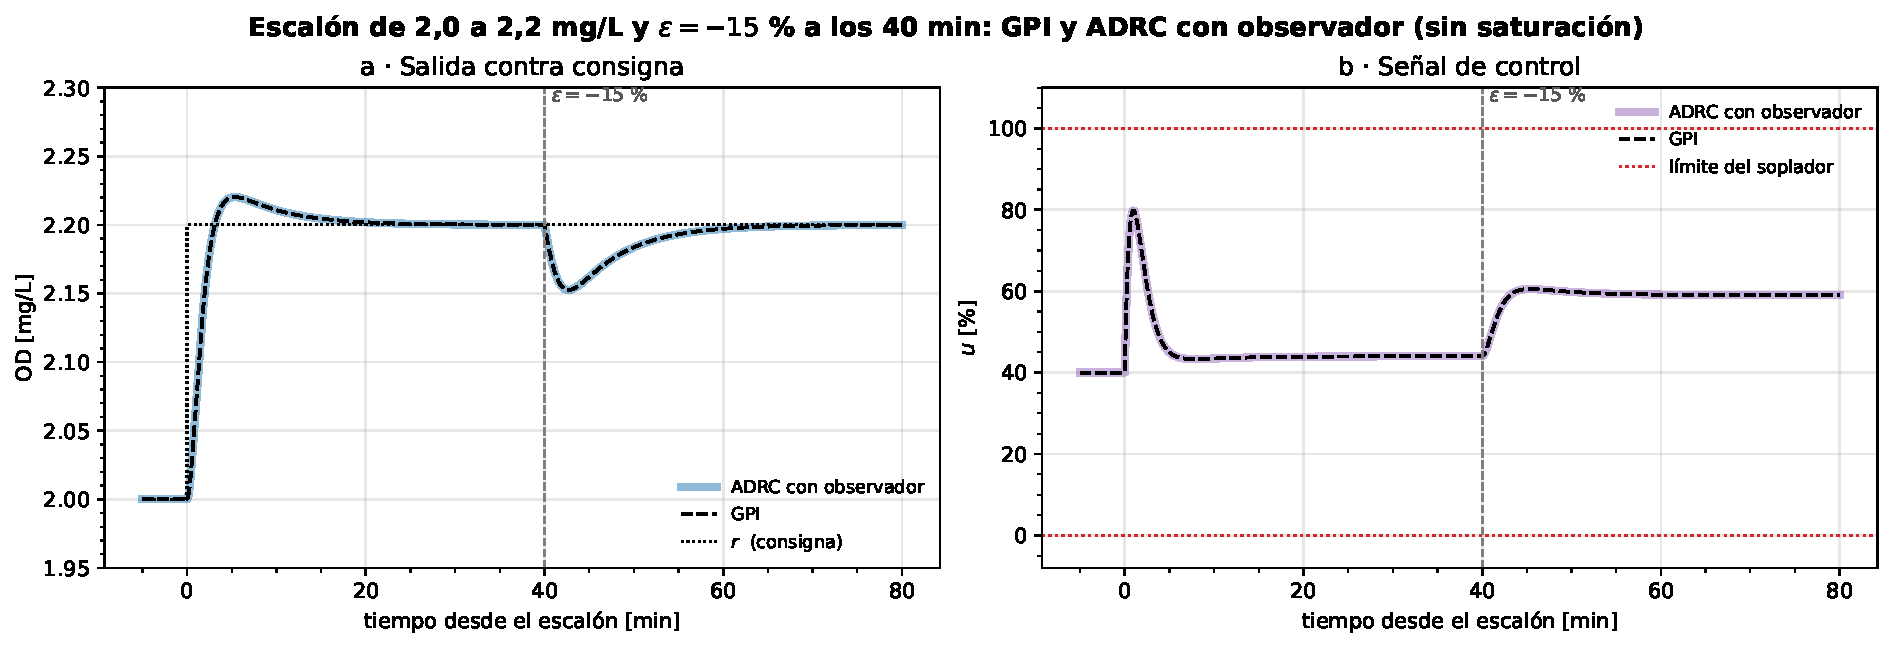
\includegraphics[width=\textwidth]{gpi_vs_adrc.pdf}
  \caption[GPI y ADRC con observador en el escalón de consigna]{Escalón de
    consigna de $2{,}0$ a $2{,}2$~mg/L y perturbación de entrada
    $\varepsilon = -15~\%$ a los $40$~min, con la planta nominal sin retardo ni
    saturación: GPI \eqref{eq:gpi_pi_filtro} y ADRC con observador
    (Sección~\ref{subsec:caso_simulacion}). (a) Salida. (b) Señal de control.}
  \label{fig:gpi_vs_adrc}
\end{figure}

Con retardo en la planta, la Figura~\ref{fig:gpi_perturbacion_retardo} repite la
entrada de la perturbación $\varepsilon = -15~\%$ con el OD en $2{,}0$~mg/L, para
$\theta$ de $0$ a $60$~s. El retardo sí afecta el rechazo: el OD baja un poco más,
de $1{,}95$ a $1{,}93$~mg/L con $60$~s, y aparece una pequeña oscilación que se
amortigua, pero la perturbación se sigue rechazando adecuadamente y la señal de
control no llega a saturarse.

\begin{figure}[H]
  \centering
  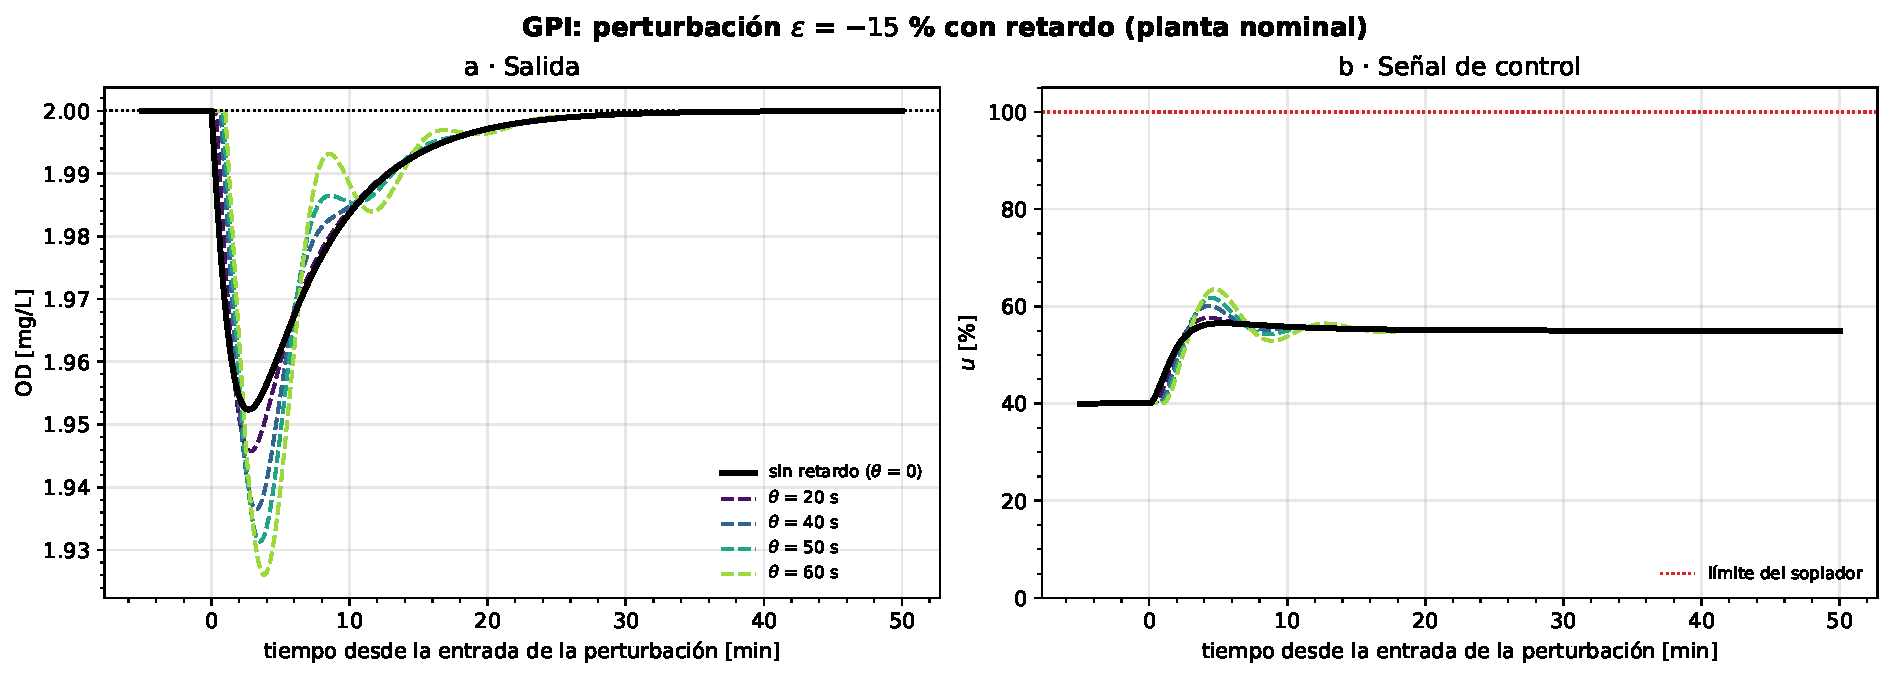
\includegraphics[width=\textwidth]{gpi_perturbacion_retardo.pdf}
  \caption[Rechazo de la perturbación con retardo con el GPI]{Entrada de una
    perturbación $\varepsilon = -15~\%$ con el OD en régimen en $2{,}0$~mg/L y la
    planta nominal con retardo $\theta$, con el GPI; en negro, sin retardo.
    (a) Salida. (b) Señal de control.}
  \label{fig:gpi_perturbacion_retardo}
\end{figure}

%--------------------------------------------------------------------
\subsection{Variación de las ganancias en el tiempo}
\label{subsec:gpi_caso_tiempo}

Para validar su comportamiento, se repite el escalón de consigna de $2{,}0$ a
$2{,}2$~mg/L, con la planta cerca del punto de operación y $u = 40~\%$, variando
cada ganancia de $1/4$ a $4$ veces su valor nominal, una a la vez y sin
saturación (Figura~\ref{fig:gpi_variacion}). El GPI se comporta como un PI con
filtro:
\begin{itemize}
  \item \textbf{$k_0$, la integral}, amplifica o disminuye el sobrepico: al
  subirla el sobrepico crece, hasta $40~\%$ con $4\,k_0$, y al bajarla
  desaparece.
  \item \textbf{$k_1$, la proporcional}, cambia el tiempo de asentamiento y las
  oscilaciones: al bajarla la respuesta oscila y tarda más en asentarse, y al
  subirla se asienta en pocos minutos, a costa de una señal de control que pasa
  del $100~\%$.
  \item \textbf{$k_2$}: al subirla, el transitorio tiene una respuesta más lenta y
  pide menos señal de control; al bajarla, el controlador es más agresivo y el
  sobrepico crece, porque además el polo del filtro se acerca al cruce de
  ganancia y le quita fase.
\end{itemize}
La Tabla~\ref{tab:gpi_transitorio} es el resumen de todo lo relacionado con las
variaciones de $k_0$ a $k_2$: sobrepico $M_p$, tiempo de asentamiento $t_s$, IAE y pico de la señal de
control (Tabla~\ref{tab:metricas}).

\begin{figure}[H]
  \centering
  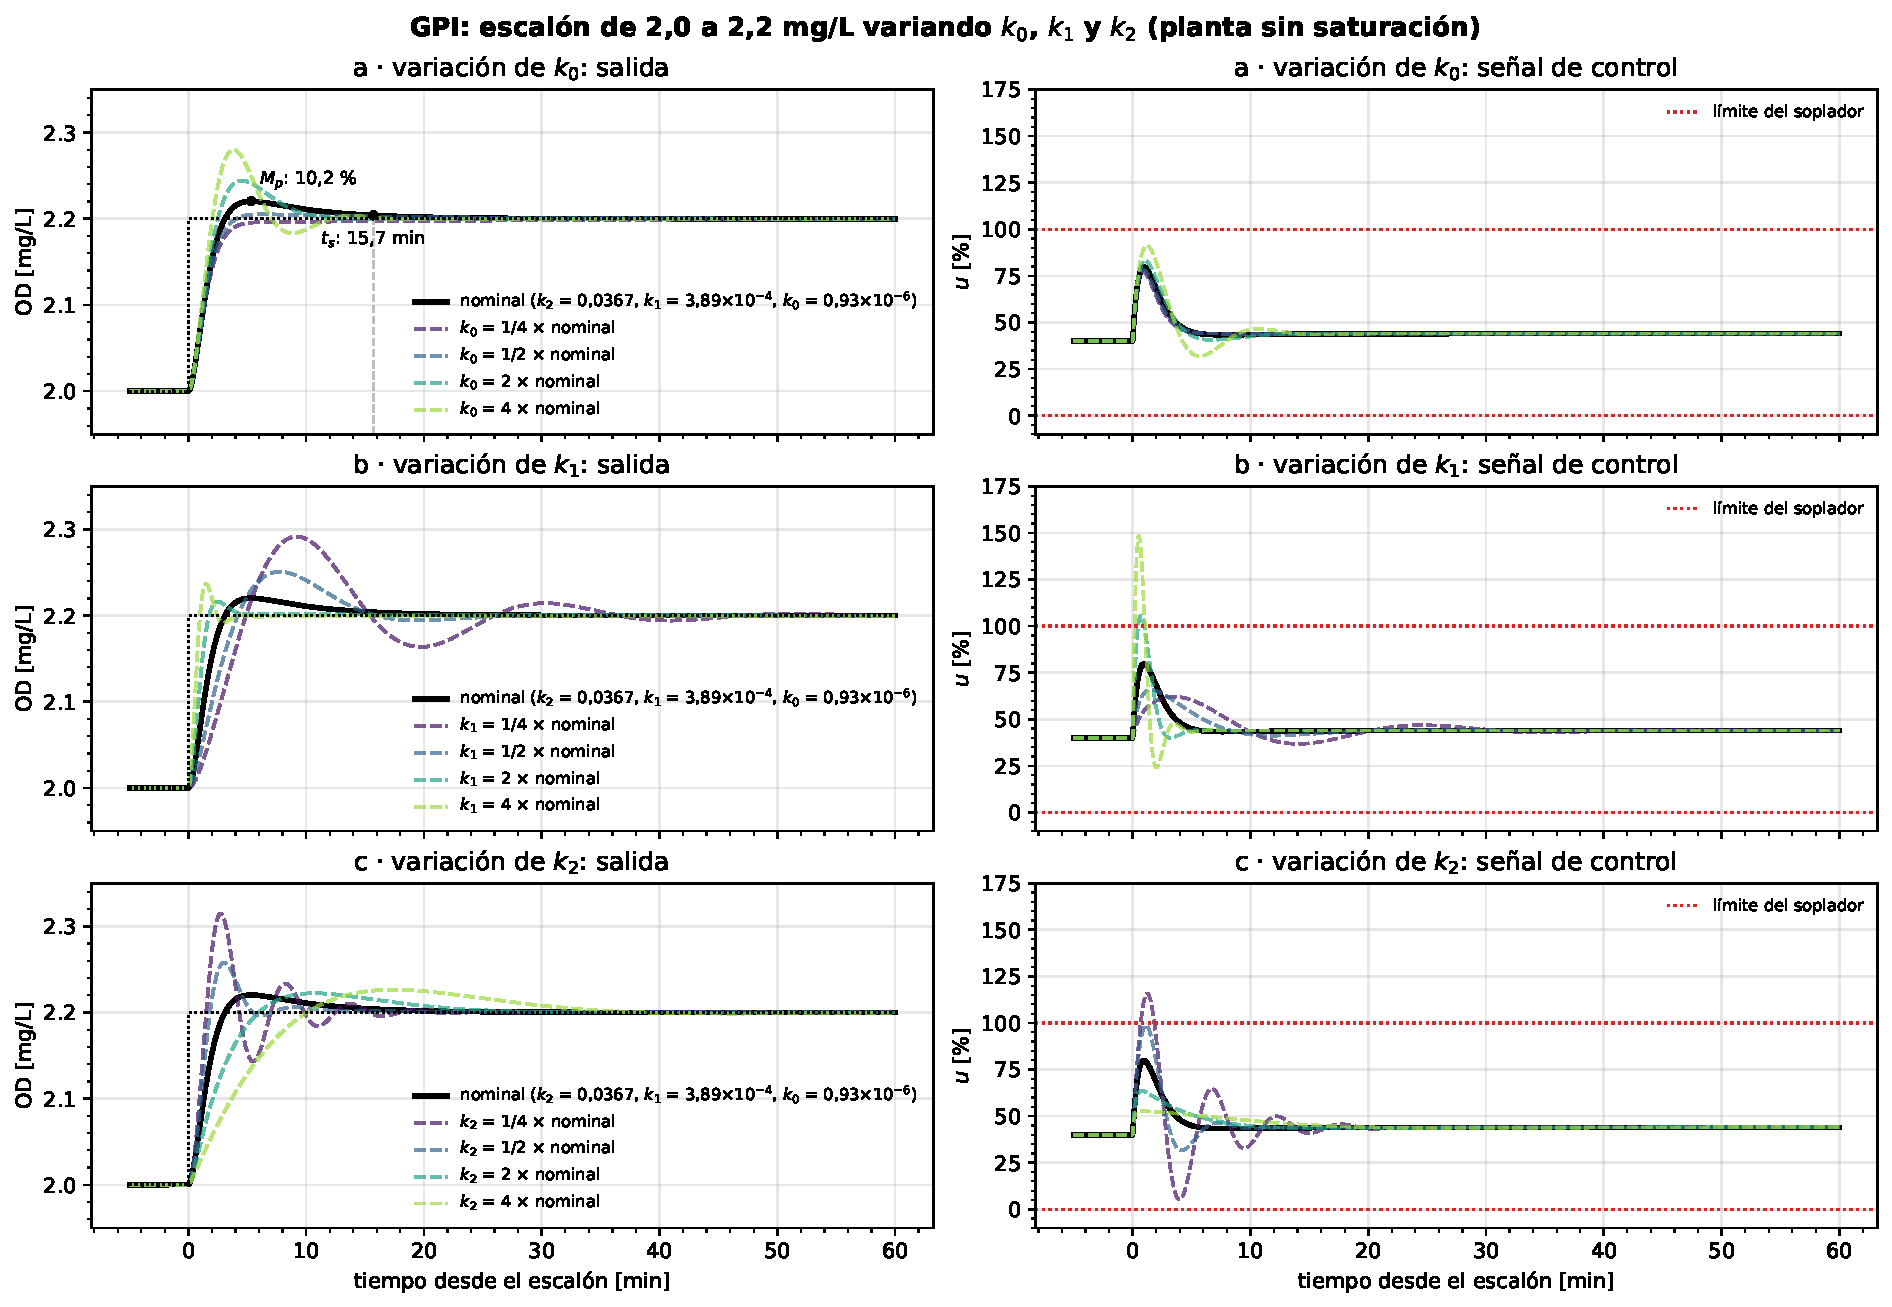
\includegraphics[width=\textwidth]{gpi_variacion_ganancias.pdf}
  \caption[Escalón de consigna con variación de las ganancias del GPI]{Escalón
    de consigna de $2{,}0$ a $2{,}2$~mg/L con el GPI y la planta, variando
    (a) $k_0$, (b) $k_1$ y (c) $k_2$. Izquierda, la salida; derecha, la señal
    de control. En negro, las ganancias nominales de la Tabla~\ref{tab:gpi_eso}.}
  \label{fig:gpi_variacion}
\end{figure}

\begin{table}[H]
\centering
\caption[Resumen del transitorio del GPI al variar sus ganancias]{Resumen del
transitorio del escalón de $2{,}0$ a $2{,}2$~mg/L de la
Figura~\ref{fig:gpi_variacion} al variar $k_0$, $k_1$ y $k_2$.}
\label{tab:gpi_transitorio}
\small
\begin{tabular}{llrrrr}
\toprule
\textbf{Ganancia} & \textbf{Factor} & $M_p$ [\%] & $t_s$ [min] & IAE [mg$\cdot$min/L] & $u_{\max}$ [\%] \\
\midrule
nominal & $1$    & $10{,}2$  & $15{,}7$  & $0{,}448$ & $79{,}8$ \\
\midrule
$k_0$   & $1/4$  & $0{,}0$   & $5{,}9$   & $0{,}423$ & $77{,}4$ \\
        & $1/2$  & $2{,}6$   & $10{,}4$  & $0{,}382$ & $78{,}2$ \\
        & $2$    & $22{,}2$  & $10{,}4$  & $0{,}458$ & $83{,}3$ \\
        & $4$    & $40{,}1$  & $11{,}3$  & $0{,}531$ & $91{,}2$ \\
\midrule
$k_1$   & $1/4$  & $45{,}9$  & $43{,}6$  & $1{,}531$ & $62{,}1$ \\
        & $1/2$  & $25{,}4$  & $22{,}4$  & $0{,}796$ & $65{,}8$ \\
        & $2$    & $8{,}2$   & $4{,}0$   & $0{,}233$ & $105{,}7$ \\
        & $4$    & $18{,}4$  & $3{,}6$   & $0{,}171$ & $148{,}4$ \\
\midrule
$k_2$   & $1/4$  & $57{,}3$  & $16{,}8$  & $0{,}604$ & $115{,}9$ \\
        & $1/2$  & $28{,}8$  & $10{,}6$  & $0{,}368$ & $98{,}7$ \\
        & $2$    & $11{,}1$  & $23{,}1$  & $0{,}722$ & $63{,}6$ \\
        & $4$    & $13{,}2$  & $33{,}1$  & $1{,}229$ & $52{,}8$ \\
\bottomrule
\end{tabular}
\end{table}

%--------------------------------------------------------------------
\subsection{Sensibilidad en lazo cerrado}
\label{subsec:gpi_caso_sensibilidad}

Para ver el efecto de las ganancias en frecuencia se usa la función de
sensibilidad en lazo cerrado frente a la perturbación total,
$e_y(s) = S_{\xi}(s)\,\xi(s)$ \eqref{eq:gpi_S}. Con los valores de la
Tabla~\ref{tab:gpi_eso},
\begin{align}
S_{\xi}(s) &= \frac{s\,(s + k_2)}{s^3 + k_2 s^2 + k_1 s + k_0}
= \frac{s\,(s + 0{,}0367)}{s^3 + 0{,}0367\,s^2 + 3{,}89\times10^{-4}\,s + 9{,}26\times10^{-7}} \nonumber\\[4pt]
&= \frac{s\,(s + 0{,}0367)}{(s + 0{,}00333)\,(s + 0{,}0167)^2} ,
\label{eq:gpi_caso_S}
\end{align}
cuyo denominador tiene los polos de diseño, en $-\omega_c$ y $-\omega_o$; con la
planta nominal el lazo cerrado los mueve un poco (Tabla~\ref{tab:caso_polos}),
pero $S_{\xi}$ no cambia, porque esa diferencia queda dentro de $\xi$.
\begin{equation}
S_{\xi}(s) \xrightarrow{\;s\to 0\;} \frac{k_2}{k_0}\,s ,
\qquad
S_{\xi}(s) \xrightarrow{\;s\to \infty\;} \frac{1}{s} .
\label{eq:gpi_caso_S_asintotas}
\end{equation}
A baja frecuencia $S_{\xi}$ crece como $(k_2/k_0)\,s$: el integrador del
controlador rechaza las perturbaciones lentas, y entre más pequeño sea
$k_2/k_0$, mejor las rechaza. A alta frecuencia tiende a $1/s$, una integral,
que es lo mismo que pasaría sin control: perturbaciones tan rápidas el
controlador ya no las alcanza a compensar, y solo las suaviza la planta. Entre
más baja esté la curva, mejor se rechaza la perturbación; $S_{\xi}$ no habla del
ruido del sensor, que entra por la medida y llega al soplador por otra función
del lazo (Figura~\ref{fig:adrc_gang_kESO}(h)). En la
Figura~\ref{fig:gpi_sensibilidad} se ve que:
\begin{itemize}
  \item con $k_0$ y $k_2$ se sube o se baja la curva a baja frecuencia: subir
  $k_0$ o bajar $k_2$ la baja y rechaza mejor las perturbaciones lentas, y lo
  contrario la sube;
  \item con $k_1$ se mueve el pico central, el de resonancia: al bajar $k_1$ el
  pico crece y la perturbación se amplifica cerca de esa frecuencia, y al
  subirlo el pico baja y se corre a frecuencias más altas.
\end{itemize}

\begin{figure}[H]
  \centering
  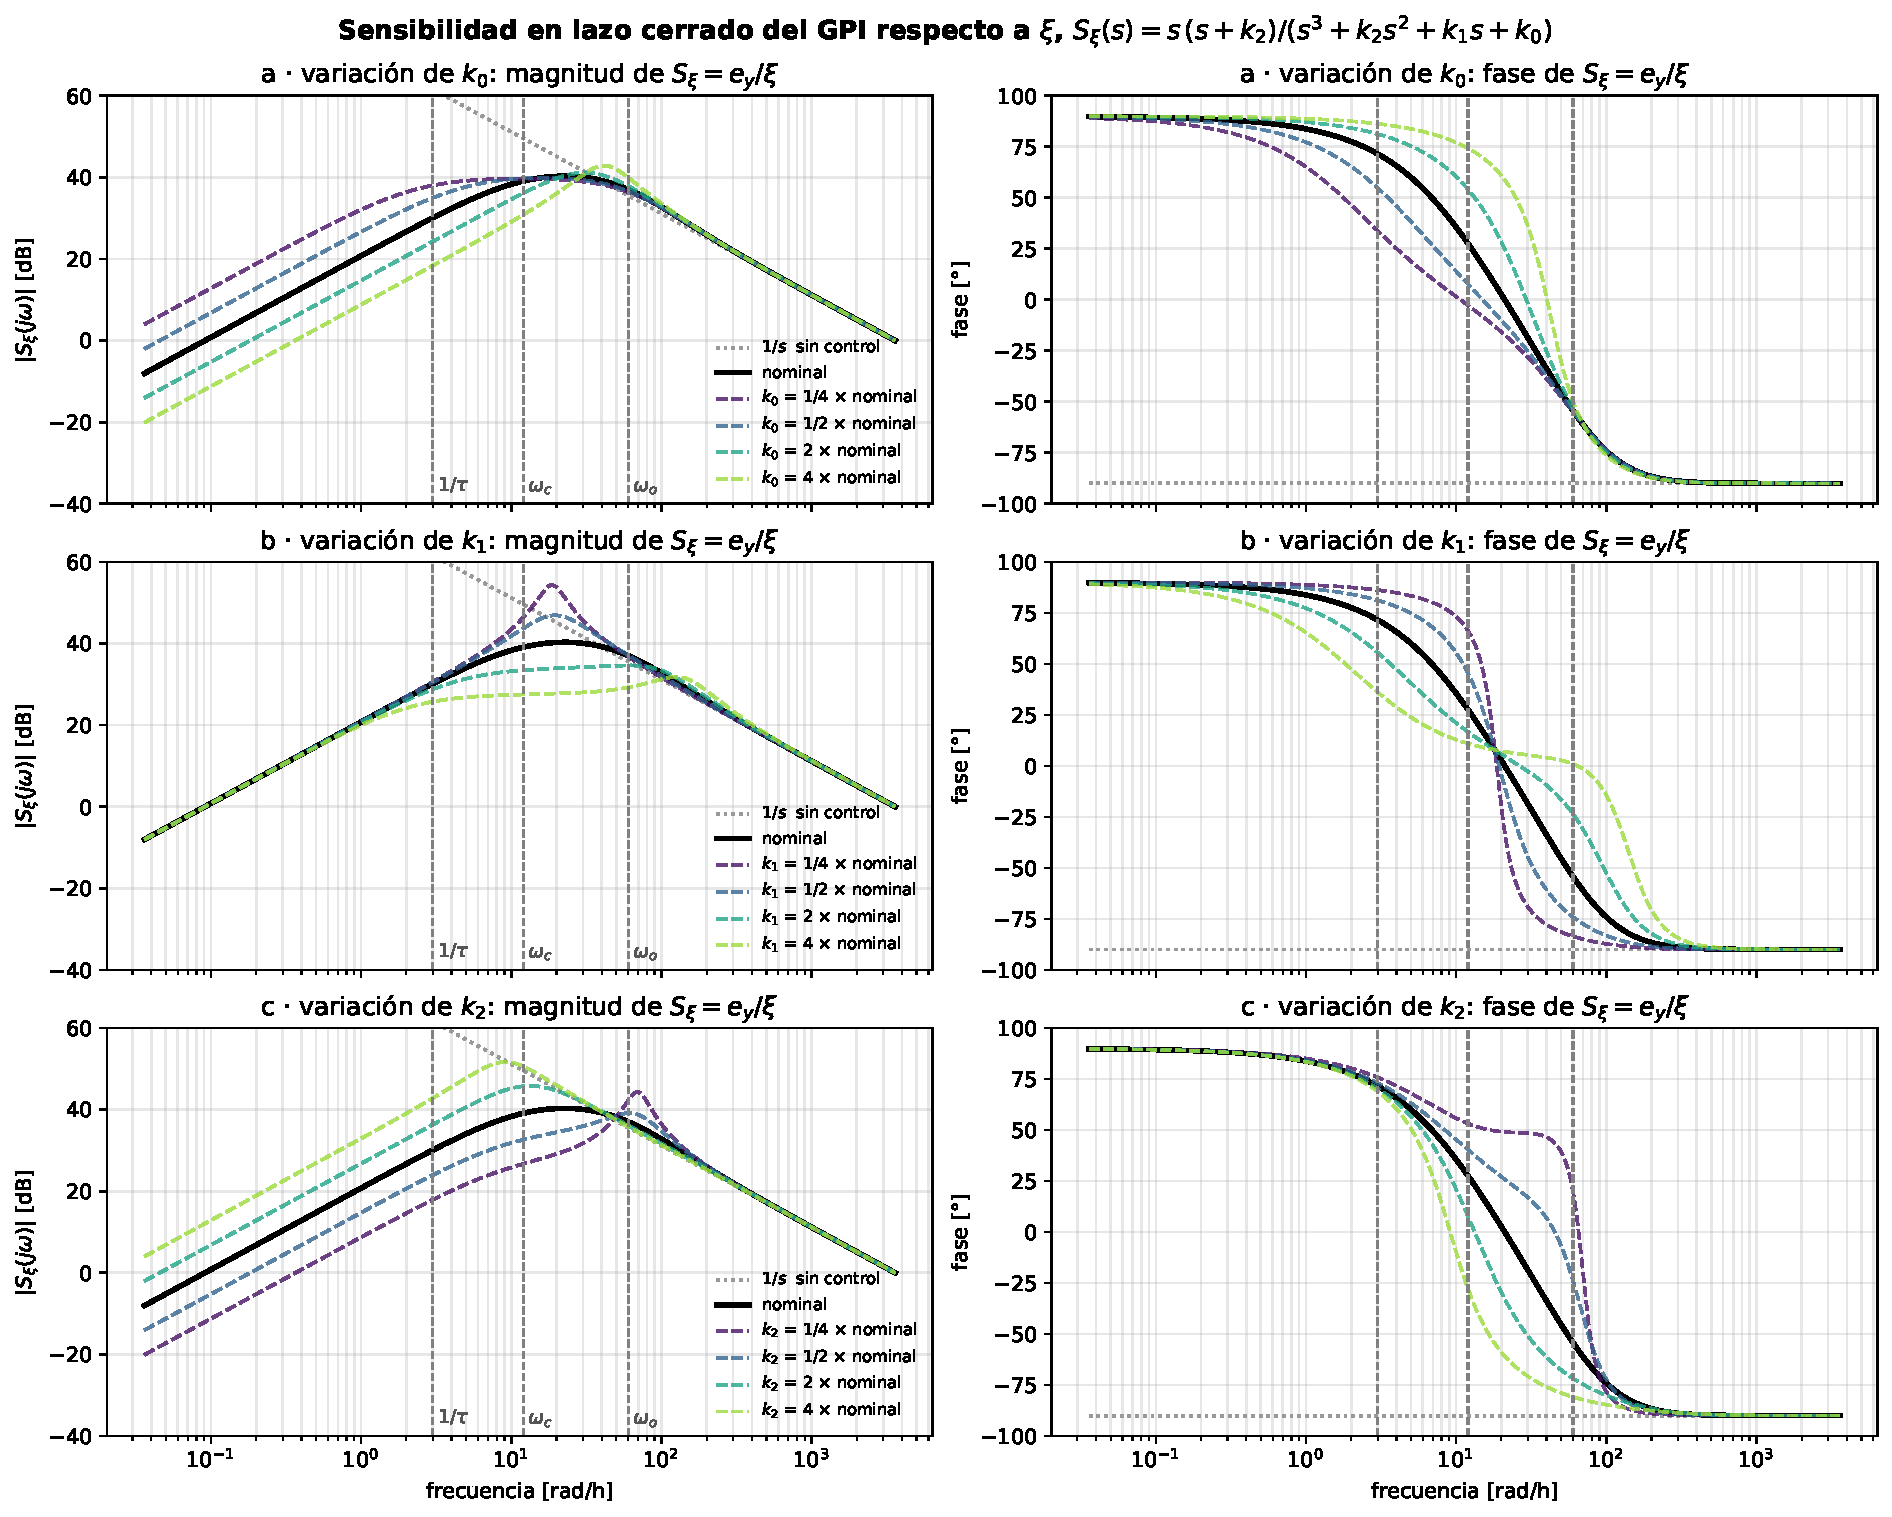
\includegraphics[width=\textwidth]{gpi_sensibilidad.pdf}
  \caption[Sensibilidad en lazo cerrado del GPI al variar sus ganancias]{Bode
    de la sensibilidad en lazo cerrado $S_{\xi}(s) = e_y/\xi$ \eqref{eq:gpi_caso_S},
    variando (a) $k_0$, (b) $k_1$ y (c) $k_2$; $\xi$ en mg/(L$\cdot$s), así que
    $|S_{\xi}|$ está en dB respecto a $1$~s. Izquierda, magnitud; derecha, fase. En
    gris punteado, $1/s$, el error sin control; las verticales marcan $1/\tau$,
    $\omega_c$ y $\omega_o$.}
  \label{fig:gpi_sensibilidad}
\end{figure}


Para ver cómo cambia la robustez con cada ganancia, la
Figura~\ref{fig:gpi_margen_fase} muestra el lazo abierto $C(s)\,G(s)$ con la
planta nominal al variar $k_0$, $k_1$ y $k_2$, con el margen de fase de cada caso.
Lo que se gana en rechazo se pierde en robustez, y se debe llegar siempre a un
equilibrio: subir $k_0$ le quita fase cerca del cruce de ganancia, y subir $k_1$ o
bajar $k_2$ lleva el cruce a frecuencias más altas; en los dos casos el margen de
fase y el retardo que aguanta el lazo tienden a bajar. Con $k_2/4$, por ejemplo, el margen
cae a unos $21^{\circ}$ y el lazo solo aguanta unos $20$~s de retardo, menos que
los $50$~s de la planta. Bajar $k_1$ tampoco ayuda, porque el pico de resonancia
que crece también le quita margen. Subir $k_2$ hace lo contrario: más margen y
más retardo tolerable, pero peor rechazo de las perturbaciones.

Estas relaciones no siempre se cumplen, porque dependen de dónde quede la frecuencia de cruce de
ganancia y de cómo se comporte la fase. Lo mejor es disminuir $k_0$, para tener un sistema más lento
y ganar margen de fase, sintonizar $k_2$ a partir del ruido que se desea filtrar, y siempre validarlo
con simulación. La Tabla~\ref{tab:gpi_frecuencia} resume las Figuras~\ref{fig:gpi_sensibilidad}
y~\ref{fig:gpi_margen_fase}.

\begin{figure}[H]
  \centering
  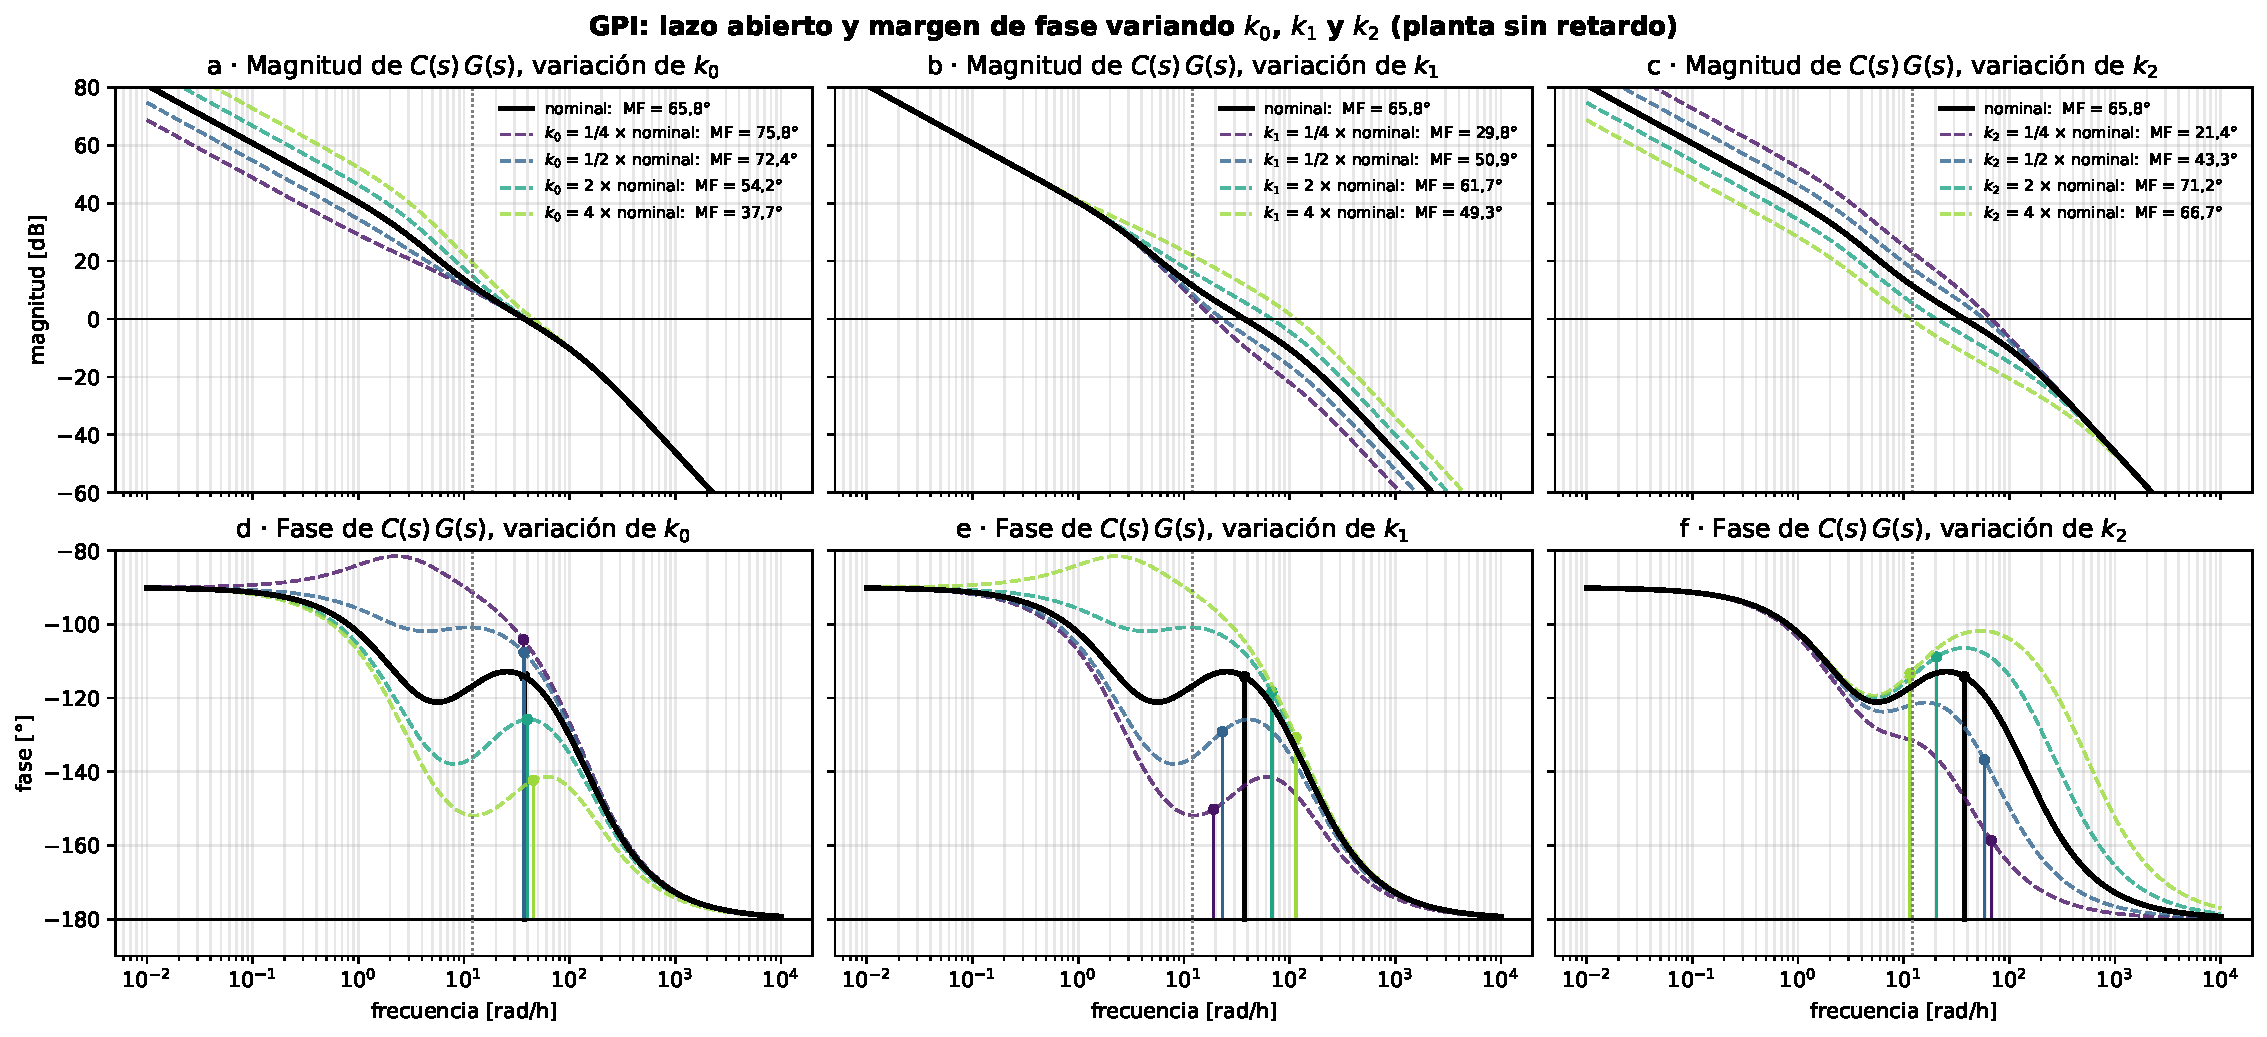
\includegraphics[width=\textwidth]{gpi_margen_fase.pdf}
  \caption[Margen de fase del GPI al variar sus ganancias]{Lazo abierto
    $C(s)\,G(s)$ con la planta nominal sin retardo, variando (a, d) $k_0$,
    (b, e) $k_1$ y (c, f) $k_2$; en negro, las ganancias nominales. Arriba, la
    magnitud; abajo, la fase, con el margen de fase como segmento vertical y su
    valor en la leyenda. La vertical punteada marca $\omega_c$.}
  \label{fig:gpi_margen_fase}
\end{figure}

\begin{table}[H]
\centering
\caption[Sensibilidad y robustez del GPI al variar sus ganancias]{Resumen de
  las Figuras~\ref{fig:gpi_sensibilidad} y~\ref{fig:gpi_margen_fase}: pico de
  $|S_{\xi}| = |e_y/\xi|$ \eqref{eq:gpi_caso_S} y su frecuencia, pendiente $k_2/k_0$
  a baja frecuencia \eqref{eq:gpi_caso_S_asintotas}, y margen de fase, retardo
  máximo y $M_s$ del lazo con la planta nominal sin retardo,
  variando una ganancia a la vez.}
\label{tab:gpi_frecuencia}
\small
\begin{tabular}{llrrrrrr}
\toprule
\textbf{Ganancia} & \textbf{Factor} & pico $|S_{\xi}|$ [dB] & en [rad/h] & $k_2/k_0$ [h] & MF [°] & $\theta_{\max}$ [s] & $M_s$ \\
\midrule
nominal & $1$ & $40{,}3$ & $22{,}6$ & $11{,}0$ & $65{,}8$ & $110$ & $1{,}202$ \\
\midrule
$k_0$ & $1/4$ & $39{,}7$ & $11{,}7$ & $44{,}0$ & $75{,}8$ & $130$ & $1{,}171$ \\
 & $1/2$ & $39{,}9$ & $16{,}3$ & $22{,}0$ & $72{,}4$ & $123$ & $1{,}180$ \\
 & $2$ & $41{,}1$ & $30{,}8$ & $5{,}5$ & $54{,}2$ & $86$ & $1{,}271$ \\
 & $4$ & $42{,}9$ & $41{,}5$ & $2{,}8$ & $37{,}7$ & $52$ & $1{,}608$ \\
\midrule
$k_1$ & $1/4$ & $54{,}3$ & $18{,}6$ & $11{,}0$ & $29{,}8$ & $98$ & $1{,}977$ \\
 & $1/2$ & $46{,}9$ & $19{,}5$ & $11{,}0$ & $50{,}9$ & $138$ & $1{,}240$ \\
 & $2$ & $34{,}6$ & $60{,}6$ & $11{,}0$ & $61{,}7$ & $57$ & $1{,}313$ \\
 & $4$ & $31{,}8$ & $125{,}4$ & $11{,}0$ & $49{,}3$ & $27$ & $1{,}516$ \\
\midrule
$k_2$ & $1/4$ & $44{,}3$ & $69{,}1$ & $2{,}8$ & $21{,}4$ & $20$ & $2{,}865$ \\
 & $1/2$ & $39{,}1$ & $61{,}0$ & $5{,}5$ & $43{,}3$ & $47$ & $1{,}627$ \\
 & $2$ & $45{,}8$ & $13{,}3$ & $22{,}0$ & $71{,}2$ & $219$ & $1{,}062$ \\
 & $4$ & $51{,}7$ & $9{,}1$ & $44{,}0$ & $66{,}7$ & $364$ & $1{,}023$ \\
\bottomrule
\end{tabular}
\end{table}



% ============================================================================
%  Capítulo 5 - Aspectos prácticos de implementación
% ============================================================================
\chapter{Aspectos prácticos de implementación}
\label{cap:implementacion}
En este capítulo se tratan algunos aspectos prácticos de implementación que se deben
considerar a la hora de utilizar el ADRC ya en la puesta en marcha, para tener el mejor
funcionamiento posible: el manejo de la saturación, el acondicionamiento de la referencia,
el manejo del ruido y la discretización, para poder usarlo en equipos digitales. Al
finalizar el capítulo se resume toda una metodología de implementación para llegar a
utilizar el ADRC desde la teoría hasta la puesta en marcha.

%--------------------------------------------------------------------
\section{Manejo de la saturación}
\label{sec:impl_saturacion}

%--------------------------------------------------------------------
\subsection{Saturación ADRC basado en observador}
\label{subsec:sat_adrc}

El soplador solo puede entregar entre $0$ y $100~\%$, así que la orden que
llega a la planta no es $u(t)$, sino su versión limitada
\cite[sec.~9.1.1]{herbst2024adrc},
\begin{equation}
u_{\mathrm{sat}}(t) = \operatorname{sat}\bigl(u(t)\bigr) =
\begin{cases}
0~\%, & u(t) < 0~\%, \\
u(t), & 0~\% \le u(t) \le 100~\%, \\
100~\%, & u(t) > 100~\%,
\end{cases}
\qquad u(t) = \frac{u_0(t)}{b_0}.
\label{eq:saturacion}
\end{equation}
Si el observador siguiera recibiendo $u_0(t)$, estimaría el efecto de una orden
que la planta no recibió: la diferencia entre $u$ y $u_{\mathrm{sat}}$
aparecería como perturbación en $\hat{\xi}$ y la ley de control la seguiría
acumulando, que es el \emph{windup} del ADRC. Para evitarlo, al observador se le
realimenta la orden aplicada, multiplicada por $b_0$ para que vuelva a las
unidades de $u_0$ (Figura~\ref{fig:adrc_saturacion}; en la Figura~\ref{fig:simulink_eso} se
muestra el mismo esquema con bloques de Simulink):
\begin{equation}
\dot{\widehat{\mathbf{X}}}(t) =
\bigl(\mathbf{A} - \mathbf{L}\,\mathbf{C}\bigr)\,\widehat{\mathbf{X}}(t)
+ \mathbf{B}\,b_0\,u_{\mathrm{sat}}(t) + \mathbf{L}\,e_y(t).
\label{eq:observador_saturacion}
\end{equation}
Así, el ADRC con observador de estado extendido trae su propio
\emph{anti-windup}: según Herbst y Madoński, realimentar la señal limitada en
lugar de $u$ es la única medida necesaria, y no añade parámetros que sintonizar
\cite[sec.~9.1.1]{herbst2024adrc}, lo que resulta en una forma muy fácil y eficiente de
manejar la saturación.


\begin{figure}[H]
  \centering
  \resizebox{\textwidth}{!}{%
  \begin{tikzpicture}[every path/.style={thick}]

    % --- Nodos principales ---
    \node[sum] (s1) at (1.4,0) {};

    \node[block, minimum width=4.4cm, minimum height=1.9cm] (obs) at (5.9,-0.4)
      {$\mathbf{A}_o\widehat{\mathbf{X}}(t) + \mathbf{B}_o \mathbf{u}_t(t)$ \\[10pt] $\mathbf{C}_o\widehat{\mathbf{X}}(t) + \mathbf{D}_o \mathbf{u}_t(t)$};
    \node[above=1pt of obs] {Observador};

    \node[block, minimum size=9mm] (K) at (9.6,0) {$-\mathbf{K}$};
    \coordinate (u0) at (10.7,0);
    \node[block, minimum size=9mm] (ib) at (11.7,0) {$1/b_0$};

    % saturacion (icono clasico de Simulink)
    \node[block, minimum size=11mm] (sat) at (13.9,0) {};
    \draw[thin, gray] ($(sat.center)+(-0.38,0)$) -- ($(sat.center)+(0.38,0)$);
    \draw[thin, gray] ($(sat.center)+(0,-0.38)$) -- ($(sat.center)+(0,0.38)$);
    \draw[line width=1.1pt] ($(sat.center)+(-0.38,-0.22)$) -- ($(sat.center)+(-0.18,-0.22)$)
                         -- ($(sat.center)+(0.18,0.22)$) -- ($(sat.center)+(0.38,0.22)$);
    \node[above=1pt of sat, font=\small] {0--100~\%};

    \coordinate (us) at (15.3,0);
    \node[sum] (s2) at (16.7,0) {};

    \node[block, minimum width=3.6cm, minimum height=1.9cm] (plant) at (20.0,0)
      {$\mathbf{A}_g \mathbf{x}_g(t) + \mathbf{B}_g \bar{u}(t)$ \\[10pt] $\mathbf{C}_g \mathbf{x}_g(t) + \mathbf{D}_g \bar{u}(t)$};

    \coordinate (yb) at (22.4,0);

    % ganancia b0 en la realimentacion hacia el observador
    \node[block, minimum size=9mm] (gb) at (9.6,-1.9) {$b_0$};

    % --- Recuadro ADRC ---
    \draw[red, dashed, thick] (3.0,1.6) rectangle (12.4,-2.6);
    \node[below left] at (12.4,1.6) {ADRC};

    % --- Señales ---
    \draw[->] (0,0) node[above right] {$r(t)$} -- (s1.west);
    \node[sgn] at ($(s1.west)+(-0.15,0.25)$) {$-$};

    \draw[->] (s1.east) -- node[above, pos=0.45] {$e_y(t)$} (obs.west |- s1);
    \draw[->] (obs.east |- K) -- node[above] {$\widehat{\mathbf{X}}(t)$} (K.west);

    \draw (K.east) -- (u0) node[above] {$u_0(t)$};
    \draw[->] (u0) -- (ib.west);
    \draw[->] (ib.east) -- node[above, pos=0.6] {$u(t)$} (sat.west);
    \draw (sat.east) -- (us) node[above] {$u_{\mathrm{sat}}(t)$};
    \fill (us) circle (1.5pt);
    \draw[->] (us) -- (s2.west);
    \node[sgn] at ($(s2.west)+(-0.2,0.25)$) {$+$};

    % u_sat -> b0 -> observador
    \draw[->] (us) -- (us |- 0,-1.9) -- (gb.east);
    \draw[->] (gb.west) -- (3.35,-1.9) node[below right] {$b_0\,u_{\mathrm{sat}}(t)$}
              -- (3.35,-0.85) -- (obs.west |- 0,-0.85);

    \draw[->] (s2 |- 0,1.6) node[above] {$\varepsilon(t)$} -- (s2.north);
    \node[sgn] at ($(s2.north)+(-0.25,0.2)$) {$+$};

    \draw[->] (s2.east) -- node[above] {$\bar{u}(t)$} (plant.west);

    \draw (plant.east) -- (yb);
    \draw[->] (yb) -- (23.5,0) node[above left] {$y(t)$};
    \fill (yb) circle (1.5pt);

    \draw[->] (yb) -- (22.4,-3.2) -- (1.4,-3.2) -- (s1.south);
    \node[sgn] at ($(s1.south)+(-0.25,-0.15)$) {$+$};
    \node[right] at ($(s1.south)+(0,-0.45)$) {$y(t)$};

  \end{tikzpicture}%
  }
  \caption[ADRC con saturación del actuador]{ADRC con saturación del actuador.
    La orden $u = u_0/b_0$ se limita entre $0$ y $100~\%$, y al observador se le
    realimenta la orden aplicada, $b_0\,u_{\mathrm{sat}}$, que está en las
    unidades de $u_0$.}
  \label{fig:adrc_saturacion}
\end{figure}

\begin{figure}[H]
  \centering
  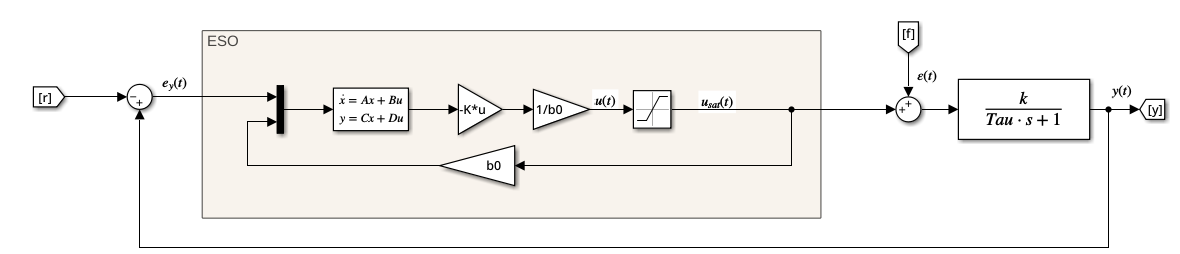
\includegraphics[width=\textwidth]{simulink_eso_saturacion.png}
  \caption[Implementación en Simulink del ADRC con saturación]{Implementación
    en Simulink del ADRC con observador, saturación del actuador y realimentación
    de la orden aplicada al observador.}
  \label{fig:simulink_eso}
\end{figure}

La Figura~\ref{fig:adrc_lazo_cerrado_saturacion} repite la simulación de la
Figura~\ref{fig:adrc_lazo_cerrado} con el soplador limitado y el observador
realimentado con $b_0\,u_{\mathrm{sat}}$. Al arrancar, el soplador se queda en
$100~\%$ unos $325$~s y el oxígeno sube más despacio (alcanza el $63~\%$ del
primer escalón en $354$~s, frente a $98$~s sin saturación), pero sin
sobreimpulso ni \emph{windup}: en cuanto la salida se acerca a la consigna, $u$
deja el límite y vuelve la dinámica diseñada. En el panel (c) se ve la perturbación exógena
aplicada y la perturbación total estimada: al entrar un cambio de referencia, el observador lo
estima como parte de la perturbación total, por lo que se ve un pico enorme que luego vuelve al
estado estacionario.


En el cambio de la referencia de $2{,}0$ a $2{,}2$~mg/L se ve el mismo comportamiento
que en el caso sin el manejo de saturación: cerca del
punto de operación de $2$~mg/L, el controlador regula y sigue cambios pequeños
de consigna sin llegar a los límites. Esta es la ventaja del esquema: sigue y
rechaza distintos tipos de señales con solo incluirlas en el modelo interno.
Su desventaja es que, con escalones grandes o una sintonía agresiva, puede
saturar el actuador. Para seguir consignas tipo escalón sin saturar, la
referencia se suaviza antes de entrar al controlador, ya sea, como se presenta en este
documento, con una curva de Bézier o con un prefiltro de la señal de consigna, de modo que la salida llegue a la consigna de forma gradual sin que la señal
de control se sature (Sección~\ref{sec:impl_referencia}).


\begin{figure}[H]
  \centering
  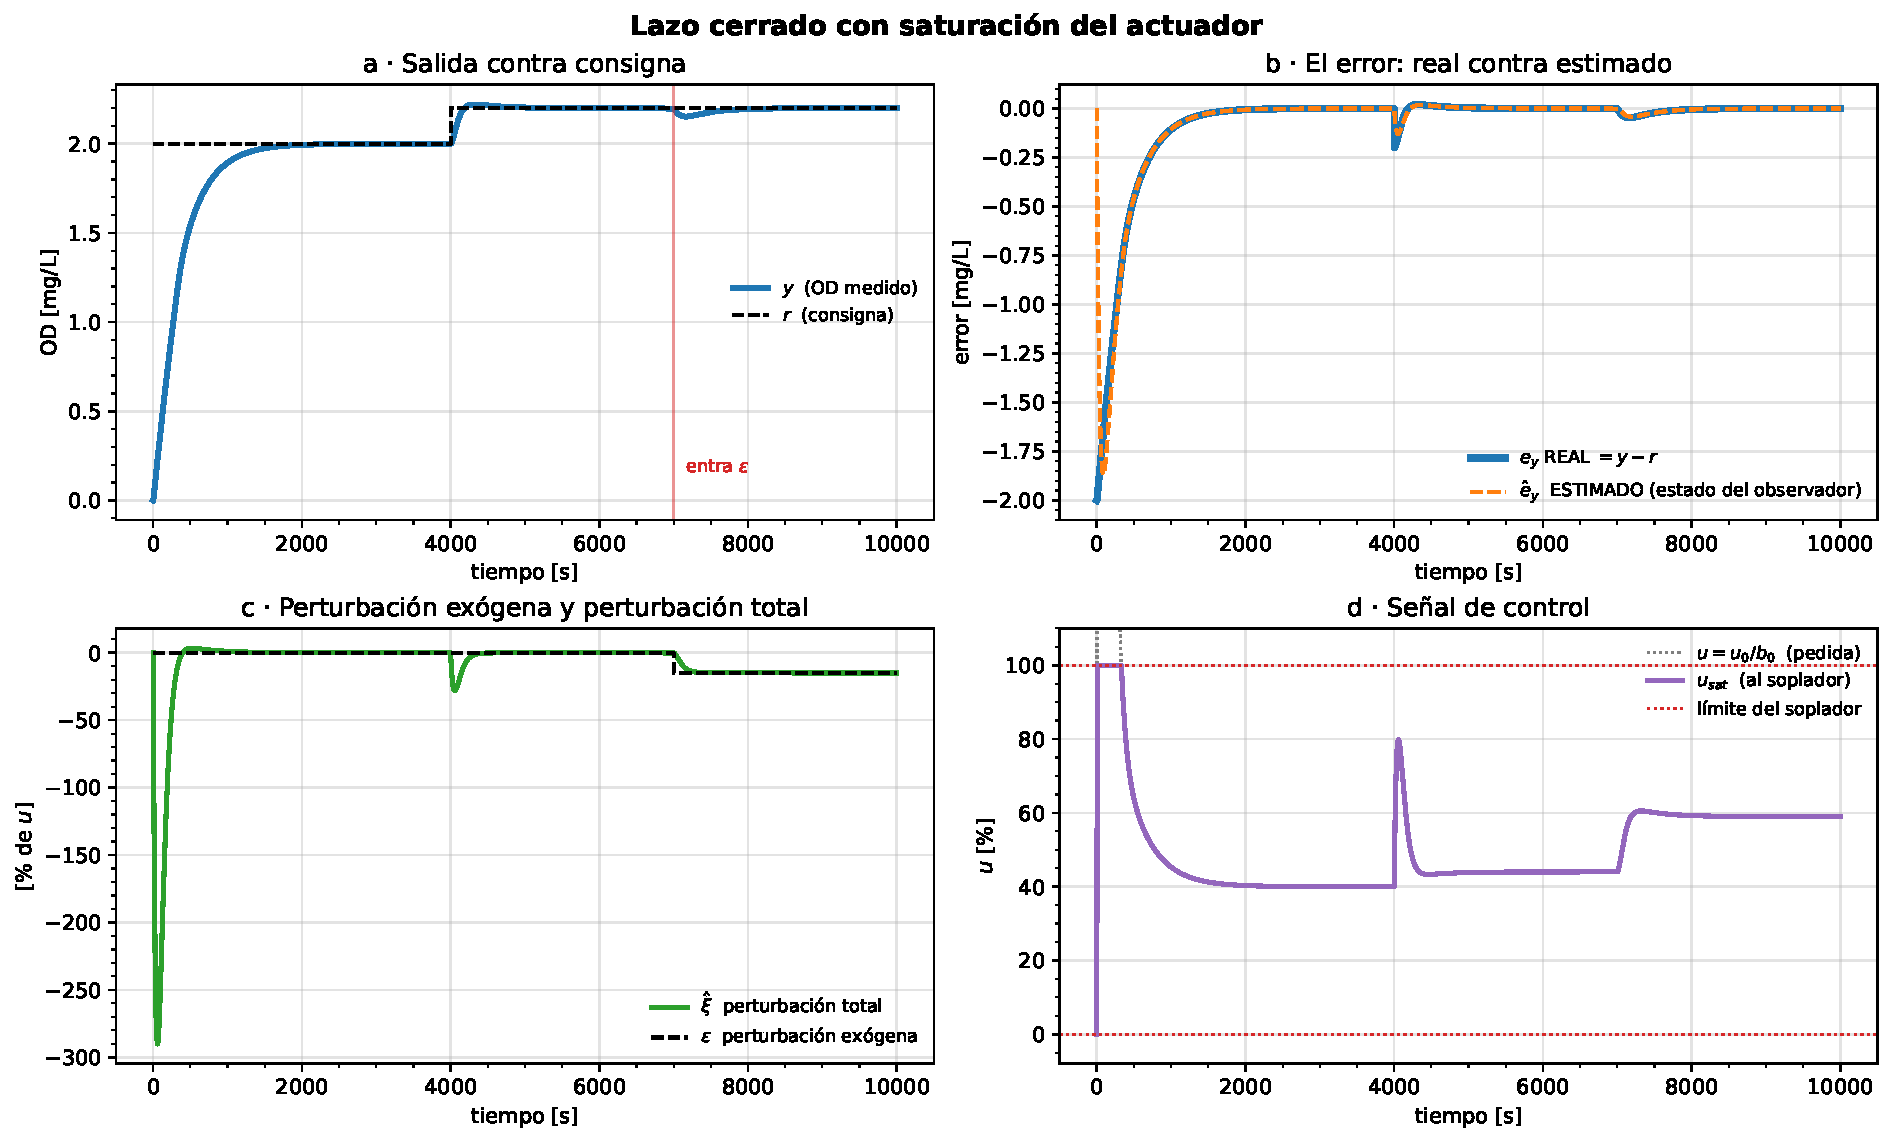
\includegraphics[width=\textwidth]{adrc_lazo_cerrado_saturacion.pdf}
  \caption[Lazo cerrado del ADRC con saturación del actuador]{Lazo cerrado del
    ADRC con la planta y el soplador limitado entre $0$ y $100~\%$.
    (a) Salida contra consigna. (b) Error de seguimiento real y estimado.
    (c) Perturbación exógena y perturbación total, en \% de $u$. (d) Orden
    pedida por el controlador y orden aplicada.}
  \label{fig:adrc_lazo_cerrado_saturacion}
\end{figure}

%--------------------------------------------------------------------
\subsection{Saturación GPI}
\label{subsec:sat_gpi}

\paragraph{Implementación con realimentación de la saturación.} Todo
controlador lineal puede escribirse como un cociente de polinomios, con $L(s)$
mónico de grado $n$ \cite[sec.~19.1.3]{levine2011handbook}, el mismo punto de partida que usan
Cortés-Romero y colaboradores para el \emph{anti-windup} de un GPI robusto
\cite{vargas2026microgrids}, mostrado con un esquema de saturación del Handbook:
\begin{equation}
u(s) = C(s)\,\bigl(-e_y(s)\bigr) = \frac{P(s)}{L(s)}\,\bigl(-e_y(s)\bigr),
\qquad L(s) = s^{n} + l_{n-1}s^{n-1} + \cdots + l_0 .
\end{equation}
Se puede implementar realimentando la señal saturada, con un polinomio mónico y estable
$E_1(s)$ del mismo grado $n$ (Figura~\ref{fig:gpi_antiwindup}), esquema obtenido de
\cite[sec.~19.1.3]{levine2011handbook}:
\begin{equation}
v(s) = \frac{P(s)}{E_1(s)}\,\bigl(-e_y(s)\bigr) - \frac{L(s) - E_1(s)}{E_1(s)}\,u_{\mathrm{sat}}(s),
\qquad u_{\mathrm{sat}}(t) = \operatorname{sat}\bigl(v(t)\bigr) .
\label{eq:aw_handbook}
\end{equation}
Cuando el actuador no se satura, $v = u_{\mathrm{sat}} = u$, y se recupera el
controlador original:
\begin{align}
u(s) &= \frac{P(s)}{E_1(s)}\,\bigl(-e_y(s)\bigr) - \frac{L(s) - E_1(s)}{E_1(s)}\,u(s) \nonumber\\[4pt]
u(s)\left[1 + \frac{L(s) - E_1(s)}{E_1(s)}\right] &= \frac{P(s)}{E_1(s)}\,\bigl(-e_y(s)\bigr) \nonumber\\[4pt]
u(s)\left[\frac{L(s)}{E_1(s)}\right] &= \frac{P(s)}{E_1(s)}\,\bigl(-e_y(s)\bigr) \nonumber\\[4pt]
u(s) &= \frac{P(s)}{L(s)}\,\bigl(-e_y(s)\bigr) .
\end{align}

\begin{figure}[H]
  \centering
  \resizebox{\textwidth}{!}{%
  \begin{tikzpicture}[every path/.style={thick}]
    \node[sum] (s1) at (1.2,0) {};
    \node[block, minimum width=2.0cm, minimum height=1.3cm] (pe) at (3.9,0)
      {$\dfrac{P(s)}{E_1(s)}$};
    \node[sum] (s2) at (6.2,0) {};

    % saturacion (icono clasico de Simulink)
    \node[block, minimum size=11mm] (sat) at (8.0,0) {};
    \draw[thin, gray] ($(sat.center)+(-0.38,0)$) -- ($(sat.center)+(0.38,0)$);
    \draw[thin, gray] ($(sat.center)+(0,-0.38)$) -- ($(sat.center)+(0,0.38)$);
    \draw[line width=1.1pt] ($(sat.center)+(-0.38,-0.22)$) -- ($(sat.center)+(-0.18,-0.22)$)
                         -- ($(sat.center)+(0.18,0.22)$) -- ($(sat.center)+(0.38,0.22)$);
    \node[above=1pt of sat, font=\small] {0--100~\%};

    \coordinate (us) at (9.6,0);
    \node[block, minimum width=2.4cm, minimum height=1.3cm] (fb) at (7.9,-1.9)
      {$\dfrac{L(s) - E_1(s)}{E_1(s)}$};
    \node[sum] (s3) at (11.4,0) {};
    \node[block, minimum width=2.4cm, minimum height=1.3cm] (plant) at (13.9,0)
      {$G(s)$};
    \coordinate (yb) at (16.1,0);

    % --- recuadro del controlador ---
    \draw[red, dashed, thick] (2.5,1.85) rectangle (10.1,-2.85);
    \node[below left] at (10.1,1.85) {GPI con \emph{anti-windup}};

    % --- señales ---
    \draw[->] (-0.3,0) node[above right] {$r(t)$} -- (s1.west);
    \node[sgn] at ($(s1.west)+(-0.15,0.25)$) {$+$};
    \draw[->] (s1.east) -- node[above, pos=0.35] {$-e_y(t)$} (pe.west);
    \draw[->] (pe.east) -- (s2.west);
    \node[sgn] at ($(s2.west)+(-0.2,0.25)$) {$+$};
    \draw[->] (s2.east) -- node[above] {$v(t)$} (sat.west);
    \draw (sat.east) -- (us);
    \fill (us) circle (1.5pt);
    \draw[->] (us) -- node[above, pos=0.62] {$u_{\mathrm{sat}}(t)$} (s3.west);
    \node[sgn] at ($(s3.west)+(-0.2,-0.25)$) {$+$};
    \draw[->] (s3 |- 0,1.6) node[above] {$\xi(t)$} -- (s3.north);
    \node[sgn] at ($(s3.north)+(0.25,0.2)$) {$+$};
    \draw[->] (s3.east) -- node[above] {$\bar{u}(t)$} (plant.west);
    \draw[->] (us) -- (us |- fb) -- (fb.east);
    \draw[->] (fb.west) -- (s2 |- fb) -- (s2.south);
    \node[sgn] at ($(s2.south)+(-0.25,-0.2)$) {$-$};
    \draw (plant.east) -- (yb);
    \draw[->] (yb) -- (17.2,0) node[above left] {$y(t)$};
    \fill (yb) circle (1.5pt);
    \draw[->] (yb) -- (16.1,-3.3) -- (1.2,-3.3) -- (s1.south);
    \node[sgn] at ($(s1.south)+(-0.25,-0.15)$) {$-$};
  \end{tikzpicture}%
  }
  \caption[GPI con realimentación de la saturación]{Implementación del GPI con
    realimentación de la saturación \cite[sec.~19.1.3]{levine2011handbook}. A
    $E_1(s)$ llega la señal aplicada $u_{\mathrm{sat}}$, no la pedida $v$.}
  \label{fig:gpi_antiwindup}
\end{figure}


\paragraph{Anti-windup escrito con las ganancias del GPI.} Para el GPI
\eqref{eq:gpi_ley}, con la planta de diseño $b_0/s$, la orden se calcula en
unidades de $u_0$ y $b_0$ solo convierte a la salida, $u = u_0/b_0$, como en el
ADRC. En unidades de $u_0$ el controlador es
\begin{equation}
C_0(s) = b_0\,C(s) = \frac{k_1 s + k_0}{s\,(s + k_2)} = \frac{P(s)}{L(s)},
\qquad
P(s) = k_1 s + k_0,
\qquad
L(s) = s^2 + k_2 s \quad (n = 2) ,
\end{equation}
y el polinomio característico del lazo es
\begin{equation}
1 + C(s)\,\frac{b_0}{s}
= 1 + \frac{1}{b_0}\,\frac{k_1 s + k_0}{s\,(s + k_2)}\cdot\frac{b_0}{s} = 0
\quad\Longrightarrow\quad
\Delta(s) = s^3 + k_2 s^2 + k_1 s + k_0 .
\end{equation}
El Handbook menciona que $E_1$ puede ser cualquier polinomio mónico y estable del mismo grado
que el denominador del controlador, $L(s)$, y recomienda que esté construido con los polos más
rápidos del lazo cerrado \cite[ec.~19.3]{levine2011handbook}. Para este primer caso, $E_1$ se eligió de forma práctica a partir de las
ganancias, sin calcular los polos, para facilitar la implementación posterior: se toma como $E_1$
el polinomio $\Delta$ sin su término independiente, dividido por $s$, es decir, un polinomio
mónico de grado $2$ construido solo con las ganancias, sin factorizar,
\begin{equation}
E_1(s) = s^2 + k_2 s + k_1 .
\label{eq:aw_E1_ganancias}
\end{equation}
Con $C = C_0/b_0$, el anti-windup \eqref{eq:aw_handbook} deja $1/b_0$ justo
después del bloque de $P/E_1$, y a la rama de realimentación llega la orden
aplicada $u_{\mathrm{sat}}$:
\begin{align}
v_1(s) &= \frac{k_1 s + k_0}{s^2 + k_2 s + k_1}\,\bigl(-e_y(s)\bigr), \nonumber\\[4pt]
v_2(s) &= \frac{\bigl[s^2 + k_2 s\bigr] - \bigl[s^2 + k_2 s + k_1\bigr]}{s^2 + k_2 s + k_1}\,u_{\mathrm{sat}}(s)
= \frac{-k_1}{s^2 + k_2 s + k_1}\,u_{\mathrm{sat}}(s), \nonumber\\[4pt]
v(s) &= \frac{v_1(s)}{b_0} - v_2(s), \qquad u_{\mathrm{sat}}(t) = \operatorname{sat}\bigl(v(t)\bigr) .
\label{eq:aw_gpi}
\end{align}
Ahora bien, $E_1$ es estable siempre que $k_2, k_1 > 0$, y
la ganancia estática de la realimentación interna es exactamente $-k_1/k_1 = -1$,
así que la acción integral se recupera sin restar números casi iguales. Si el
actuador no se satura, $u_{\mathrm{sat}} = v$ y el lazo vuelve a
$u(s) = \frac{1}{b_0}\bigl(P(s)/L(s)\bigr)\bigl(-e_y(s)\bigr) = C(s)\bigl(-e_y(s)\bigr)$.

\begin{figure}[H]
  \centering
  \resizebox{\textwidth}{!}{%
  \begin{tikzpicture}[every path/.style={thick}]
    \node[sum] (s1) at (1.2,0) {};
    \node[block, minimum width=3.0cm, minimum height=1.3cm] (pe) at (4.7,0)
      {$\dfrac{k_1 s + k_0}{s^2 + k_2 s + k_1}$};
    \node[block, minimum size=9mm] (ib) at (7.8,0) {$1/b_0$};
    \node[sum] (s2) at (9.3,0) {};

    % saturacion (icono clasico de Simulink)
    \node[block, minimum size=11mm] (sat) at (11.0,0) {};
    \draw[thin, gray] ($(sat.center)+(-0.38,0)$) -- ($(sat.center)+(0.38,0)$);
    \draw[thin, gray] ($(sat.center)+(0,-0.38)$) -- ($(sat.center)+(0,0.38)$);
    \draw[line width=1.1pt] ($(sat.center)+(-0.38,-0.22)$) -- ($(sat.center)+(-0.18,-0.22)$)
                         -- ($(sat.center)+(0.18,0.22)$) -- ($(sat.center)+(0.38,0.22)$);
    \node[above=1pt of sat, font=\small] {0--100~\%};

    \coordinate (us) at (12.8,0);
    \node[block, minimum width=2.6cm, minimum height=1.3cm] (fb) at (11.0,-1.9)
      {$\dfrac{-k_1}{s^2 + k_2 s + k_1}$};
    \node[sum] (s3) at (14.2,0) {};
    \node[block, minimum width=2.4cm, minimum height=1.3cm] (plant) at (16.7,0)
      {$\dfrac{k_{dc}}{\tau s + 1}$};
    \node[above=1pt of plant] {$G(s)$};
    \coordinate (yb) at (18.8,0);

    % --- recuadro del controlador ---
    \draw[red, dashed, thick] (2.7,1.7) rectangle (13.1,-2.9);
    \node[below left] at (13.1,1.7) {GPI};

    % --- señales ---
    \draw[->] (-0.3,0) node[above right] {$r(t)$} -- (s1.west);
    \node[sgn] at ($(s1.west)+(-0.15,0.25)$) {$+$};
    \draw[->] (s1.east) -- node[above, pos=0.4] {$-e_y(t)$} (pe.west);
    \draw[->] (pe.east) -- node[above] {$v_1(t)$} (ib.west);
    \draw[->] (ib.east) -- (s2.west);
    \node[sgn] at ($(s2.west)+(-0.2,0.25)$) {$+$};
    \draw[->] (s2.east) -- node[above] {$v(t)$} (sat.west);
    \draw (sat.east) -- node[above] {$u_{\mathrm{sat}}(t)$} (us);
    \fill (us) circle (1.5pt);
    \draw[->] (us) -- (s3.west);
    \node[sgn] at ($(s3.west)+(-0.2,-0.25)$) {$+$};
    \draw[->] (s3 |- 0,1.6) node[above] {$\varepsilon(t)$} -- (s3.north);
    \node[sgn] at ($(s3.north)+(-0.25,0.2)$) {$+$};
    \draw[->] (s3.east) -- node[above] {$\bar{u}(t)$} (plant.west);
    \draw[->] (us) -- (us |- fb) -- (fb.east);
    \draw[->] (fb.west) -- (s2 |- fb) -- node[left, pos=0.5] {$v_2(t)$} (s2.south);
    \node[sgn] at ($(s2.south)+(0.25,-0.2)$) {$-$};
    \draw (plant.east) -- (yb);
    \draw[->] (yb) -- (19.9,0) node[above left] {$y(t)$};
    \fill (yb) circle (1.5pt);
    \draw[->] (yb) -- (18.8,-3.4) -- (1.2,-3.4) -- (s1.south);
    \node[sgn] at ($(s1.south)+(-0.25,-0.15)$) {$-$};
  \end{tikzpicture}%
  }
  \caption[GPI con realimentación de la saturación escrito con sus
    ganancias]{GPI con realimentación de la saturación escrito con sus
    ganancias, según \eqref{eq:aw_gpi}: $v = v_1/b_0 - v_2$, con
    $E_1(s) = s^2 + k_2 s + k_1$ en los dos bloques. $1/b_0$ va después del
    bloque $P/E_1$ ($u = u_0/b_0$) y a la rama de realimentación llega la señal
    aplicada $u_{\mathrm{sat}}$.}
  \label{fig:gpi_antiwindup_ganancias}
\end{figure}

\paragraph{Anti-windup escrito con el polinomio del observador.} Como $E_1$ es de libre
elección, también se puede tomar del polinomio característico factorizado. Con las ganancias en
función de los anchos de banda (Tabla~\ref{tab:gpi_eso}),
\begin{equation}
k_2 = \omega_c + 2\omega_o, \qquad k_1 = \omega_o\,(\omega_o + 2\omega_c), \qquad k_0 = \omega_c\,\omega_o^2,
\end{equation}
el polinomio característico se separa en la parte del controlador y la del observador,
\begin{equation}
\Delta(s) = s^3 + k_2 s^2 + k_1 s + k_0 = (s + \omega_c)\,(s + \omega_o)^2 ,
\end{equation}
y se toma como $E_1$ la parte del observador,
\begin{equation}
E_1(s) = (s + \omega_o)^2 = s^2 + 2\omega_o\,s + \omega_o^2 = s^2 + l_1 s + l_2 .
\end{equation}
Con $P(s) = k_1 s + k_0$ y $L(s) = s^2 + k_2 s$, el anti-windup \eqref{eq:aw_handbook} queda
\begin{align}
v_1(s) &= \frac{\omega_o\bigl[(\omega_o + 2\omega_c)\,s + \omega_c\,\omega_o\bigr]}{(s + \omega_o)^2}\,\bigl(-e_y(s)\bigr), \nonumber\\[4pt]
v_2(s) &= \frac{\bigl[s^2 + (\omega_c + 2\omega_o)\,s\bigr] - \bigl[s^2 + 2\omega_o\,s + \omega_o^2\bigr]}{(s + \omega_o)^2}\,u_{\mathrm{sat}}(s)
= \frac{\omega_c\,s - \omega_o^2}{(s + \omega_o)^2}\,u_{\mathrm{sat}}(s), \nonumber\\[4pt]
v(s) &= \frac{v_1(s)}{b_0} - v_2(s), \qquad u_{\mathrm{sat}}(t) = \operatorname{sat}\bigl(v(t)\bigr)
\label{eq:aw_gpi_wo}
\end{align}
(Figura~\ref{fig:gpi_antiwindup_wo}). Este $E_1$ es estable siempre, con el polo
doble en $-\omega_o$, y la ganancia estática de la realimentación interna también
es $-\omega_o^2/\omega_o^2 = -1$. Con él, el GPI con anti-windup es exactamente el
ADRC con observador realimentado con $b_0\,u_{\mathrm{sat}}$
(Sección~\ref{subsec:sat_adrc}), y en el arranque de la
Figura~\ref{fig:sat_arranque} las dos respuestas coinciden exactamente.

Si en cambio se usa el $E_1$ escrito con las ganancias \eqref{eq:aw_E1_ganancias},
la diferencia solo aparece cuando el sistema se satura: la saturación se maneja con
una dinámica un poco distinta. Cualquier $E_1$ es válido siempre que sea estable y
del mismo orden que el denominador del controlador; la versión exacta, la que
coincide con el ADRC, es la escrita con las ganancias del observador. Además, la
Figura~\ref{fig:sat_arranque} muestra el GPI sin anti-windup: al saturarse, la
dinámica se afecta por completo y aparecen sobrepicos enormes. 


\begin{figure}[H]
  \centering
  \resizebox{\textwidth}{!}{%
  \begin{tikzpicture}[every path/.style={thick}]
    \node[sum] (s1) at (1.0,0) {};
    \node[block, minimum width=3.6cm, minimum height=1.3cm] (pe) at (5.0,0)
      {$\dfrac{\omega_o\bigl[(\omega_o + 2\omega_c)\,s + \omega_c\omega_o\bigr]}{(s + \omega_o)^2}$};
    \node[above=1pt of pe] {$H_1(s)$};
    \node[block, minimum size=9mm] (ib) at (8.9,0) {$1/b_0$};
    \node[sum] (s2) at (10.4,0) {};

    % saturacion (icono clasico de Simulink)
    \node[block, minimum size=11mm] (sat) at (12.1,0) {};
    \draw[thin, gray] ($(sat.center)+(-0.38,0)$) -- ($(sat.center)+(0.38,0)$);
    \draw[thin, gray] ($(sat.center)+(0,-0.38)$) -- ($(sat.center)+(0,0.38)$);
    \draw[line width=1.1pt] ($(sat.center)+(-0.38,-0.22)$) -- ($(sat.center)+(-0.18,-0.22)$)
                         -- ($(sat.center)+(0.18,0.22)$) -- ($(sat.center)+(0.38,0.22)$);
    \node[above=1pt of sat, font=\small] {0--100~\%};

    \coordinate (us) at (14.0,0);
    \node[block, minimum width=2.6cm, minimum height=1.3cm] (fb) at (12.1,-1.9)
      {$\dfrac{\omega_c\,s - \omega_o^2}{(s + \omega_o)^2}$};
    \node[below=1pt of fb] {$H_2(s)$};
    \node[sum] (s3) at (15.5,0) {};
    \node[block, minimum width=2.4cm, minimum height=1.3cm] (plant) at (18.0,0)
      {$\dfrac{k_{dc}}{\tau s + 1}$};
    \node[above=1pt of plant] {$G(s)$};
    \coordinate (yb) at (20.1,0);

    % --- recuadro del controlador ---
    \draw[red, dashed, thick] (2.2,1.75) rectangle (14.4,-3.2);
    \node[below left] at (14.4,1.75) {GPI};

    % --- señales ---
    \draw[->] (-0.5,0) node[above right] {$r(t)$} -- (s1.west);
    \node[sgn] at ($(s1.west)+(-0.15,0.25)$) {$+$};
    \draw[->] (s1.east) -- node[above, pos=0.35] {$-e_y(t)$} (pe.west);
    \draw[->] (pe.east) -- node[above] {$v_1(t)$} (ib.west);
    \draw[->] (ib.east) -- (s2.west);
    \node[sgn] at ($(s2.west)+(-0.2,0.25)$) {$+$};
    \draw[->] (s2.east) -- node[above] {$v(t)$} (sat.west);
    \draw (sat.east) -- node[above] {$u_{\mathrm{sat}}(t)$} (us);
    \fill (us) circle (1.5pt);
    \draw[->] (us) -- (s3.west);
    \node[sgn] at ($(s3.west)+(-0.2,-0.25)$) {$+$};
    \draw[->] (s3 |- 0,1.6) node[above] {$\varepsilon(t)$} -- (s3.north);
    \node[sgn] at ($(s3.north)+(-0.25,0.2)$) {$+$};
    \draw[->] (s3.east) -- node[above] {$\bar{u}(t)$} (plant.west);
    \draw[->] (us) -- (us |- fb) -- (fb.east);
    \draw[->] (fb.west) -- (s2 |- fb) -- node[left, pos=0.5] {$v_2(t)$} (s2.south);
    \node[sgn] at ($(s2.south)+(0.25,-0.2)$) {$-$};
    \draw (plant.east) -- (yb);
    \draw[->] (yb) -- (21.2,0) node[above left] {$y(t)$};
    \fill (yb) circle (1.5pt);
    \draw[->] (yb) -- (20.1,-3.7) -- (1.0,-3.7) -- (s1.south);
    \node[sgn] at ($(s1.south)+(-0.25,-0.15)$) {$-$};
  \end{tikzpicture}%
  }
  \caption[GPI con realimentación de la saturación escrito con el observador]{GPI con
    realimentación de la saturación escrito con el polinomio del observador, según
    \eqref{eq:aw_gpi_wo}: $v = v_1/b_0 - v_2$, con $E_1(s) = (s + \omega_o)^2$ en los dos
    bloques.}
  \label{fig:gpi_antiwindup_wo}
\end{figure}
Seguidamente, la Figura~\ref{fig:simulink_gpi} presenta el mismo esquema, pero
realizado en Simulink, con el objetivo de validar cada una de las funciones de
transferencia en continuo y simplificar un poco el esfuerzo de ver las señales al
momento de variar los controladores.

\begin{figure}[H]
  \centering
  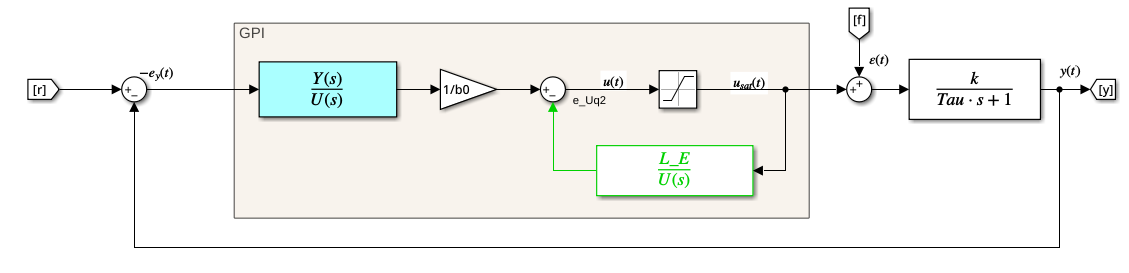
\includegraphics[width=\textwidth]{simulink_gpi_antiwindup.png}
  \caption[Implementación en Simulink del GPI con anti-windup]{Implementación en
    Simulink del GPI con realimentación de la saturación.}
  \label{fig:simulink_gpi}
\end{figure}

\begin{figure}[H]
  \centering
  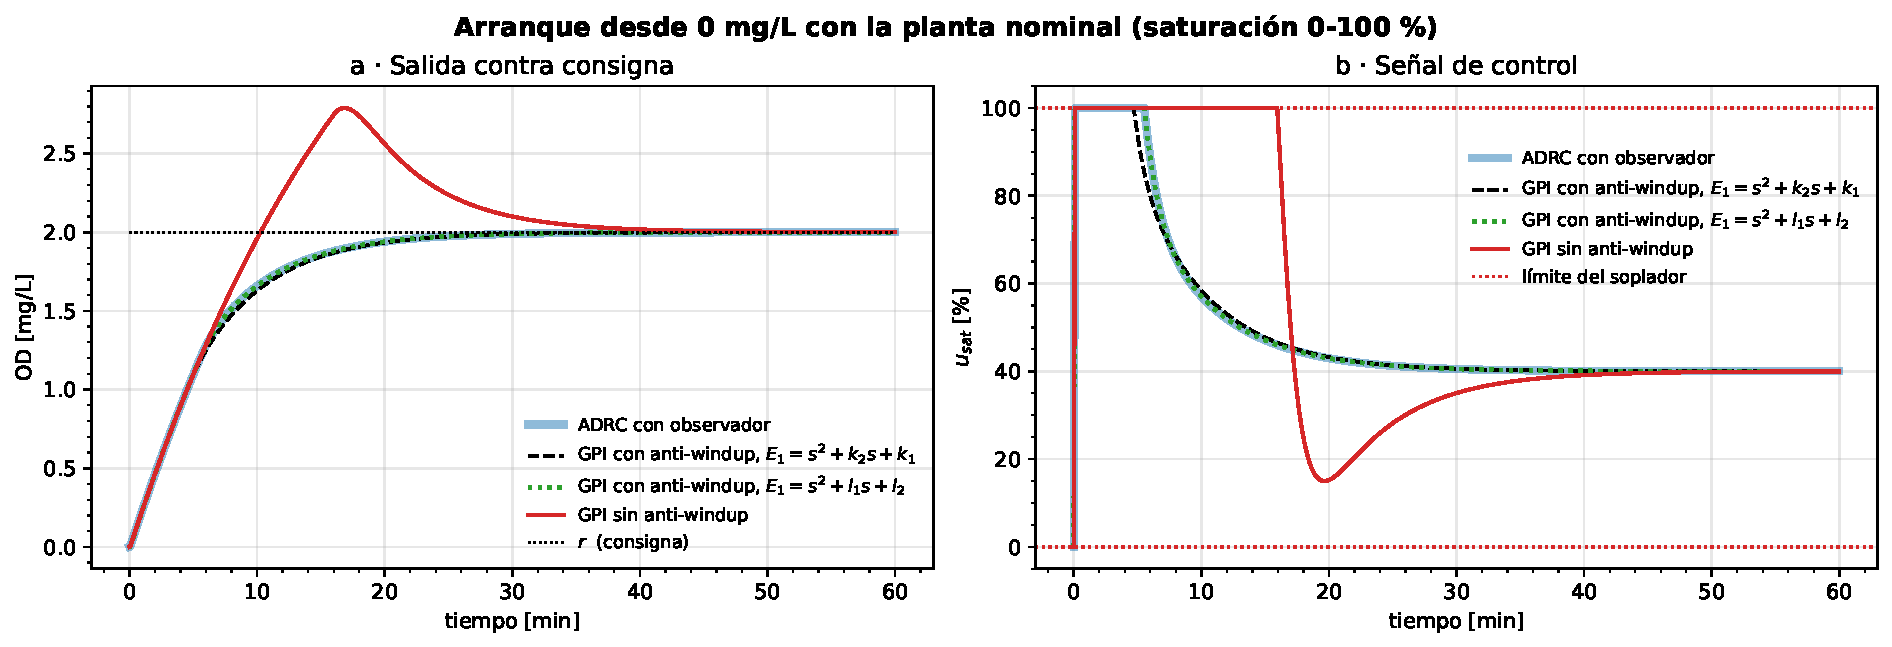
\includegraphics[width=\textwidth]{saturacion_arranque.pdf}
  \caption[Arranque desde cero con saturación]{Arranque desde $0$~mg/L con la
    planta nominal y el soplador limitado entre $0$ y $100~\%$: ADRC con
    observador, GPI con \emph{anti-windup} con $E_1 = s^2 + k_2 s + k_1$ y con
    el polinomio del observador, $E_1 = s^2 + l_1 s + l_2$, y GPI sin
    \emph{anti-windup}. (a) Salida contra consigna. (b) Señal de control.}
  \label{fig:sat_arranque}
\end{figure}

%--------------------------------------------------------------------
\subsection{Variación de los parámetros de la planta con saturación}
\label{subsec:sat_variacion}

Se repiten las variaciones de la Sección~\ref{subsec:caso_variacion} con el
soplador limitado entre $0$ y $100~\%$, para el GPI con realimentación de la
saturación \eqref{eq:aw_gpi} y las ganancias nominales
(Figura~\ref{fig:sat_adrc_gpi_variacion}). El ADRC con observador
(Sección~\ref{subsec:sat_adrc}) da prácticamente las mismas respuestas, así que
solo se muestra el GPI. Al retardo se le añade un caso
extremo, $\theta = 100$~s, el doble del de diseño y cerca del margen de retardo
de $110$~s (Sección~\ref{subsec:caso_margenes}): el oxígeno sube hasta
$2{,}42$~mg/L y el soplador llega a $100~\%$ y a $0~\%$, pero con la
realimentación de la saturación el controlador no se desestabiliza,
y la oscilación se amortigua lentamente. En caso de que la ganancia de la planta sea muy pequeña
(caso $K_{dc} = 0{,}022$ de la Figura~\ref{fig:sat_adrc_gpi_variacion}(a)), el controlador se
mantiene saturado, es decir, el sistema no llega a la referencia; y cuando el controlador vuelva a
responder, la salida se irá acercando lentamente a la referencia a medida que el sistema se
recupere, sin sobrepicos agresivos ni enormes, gracias al \emph{anti-windup}.


\begin{figure}[H]
  \centering
  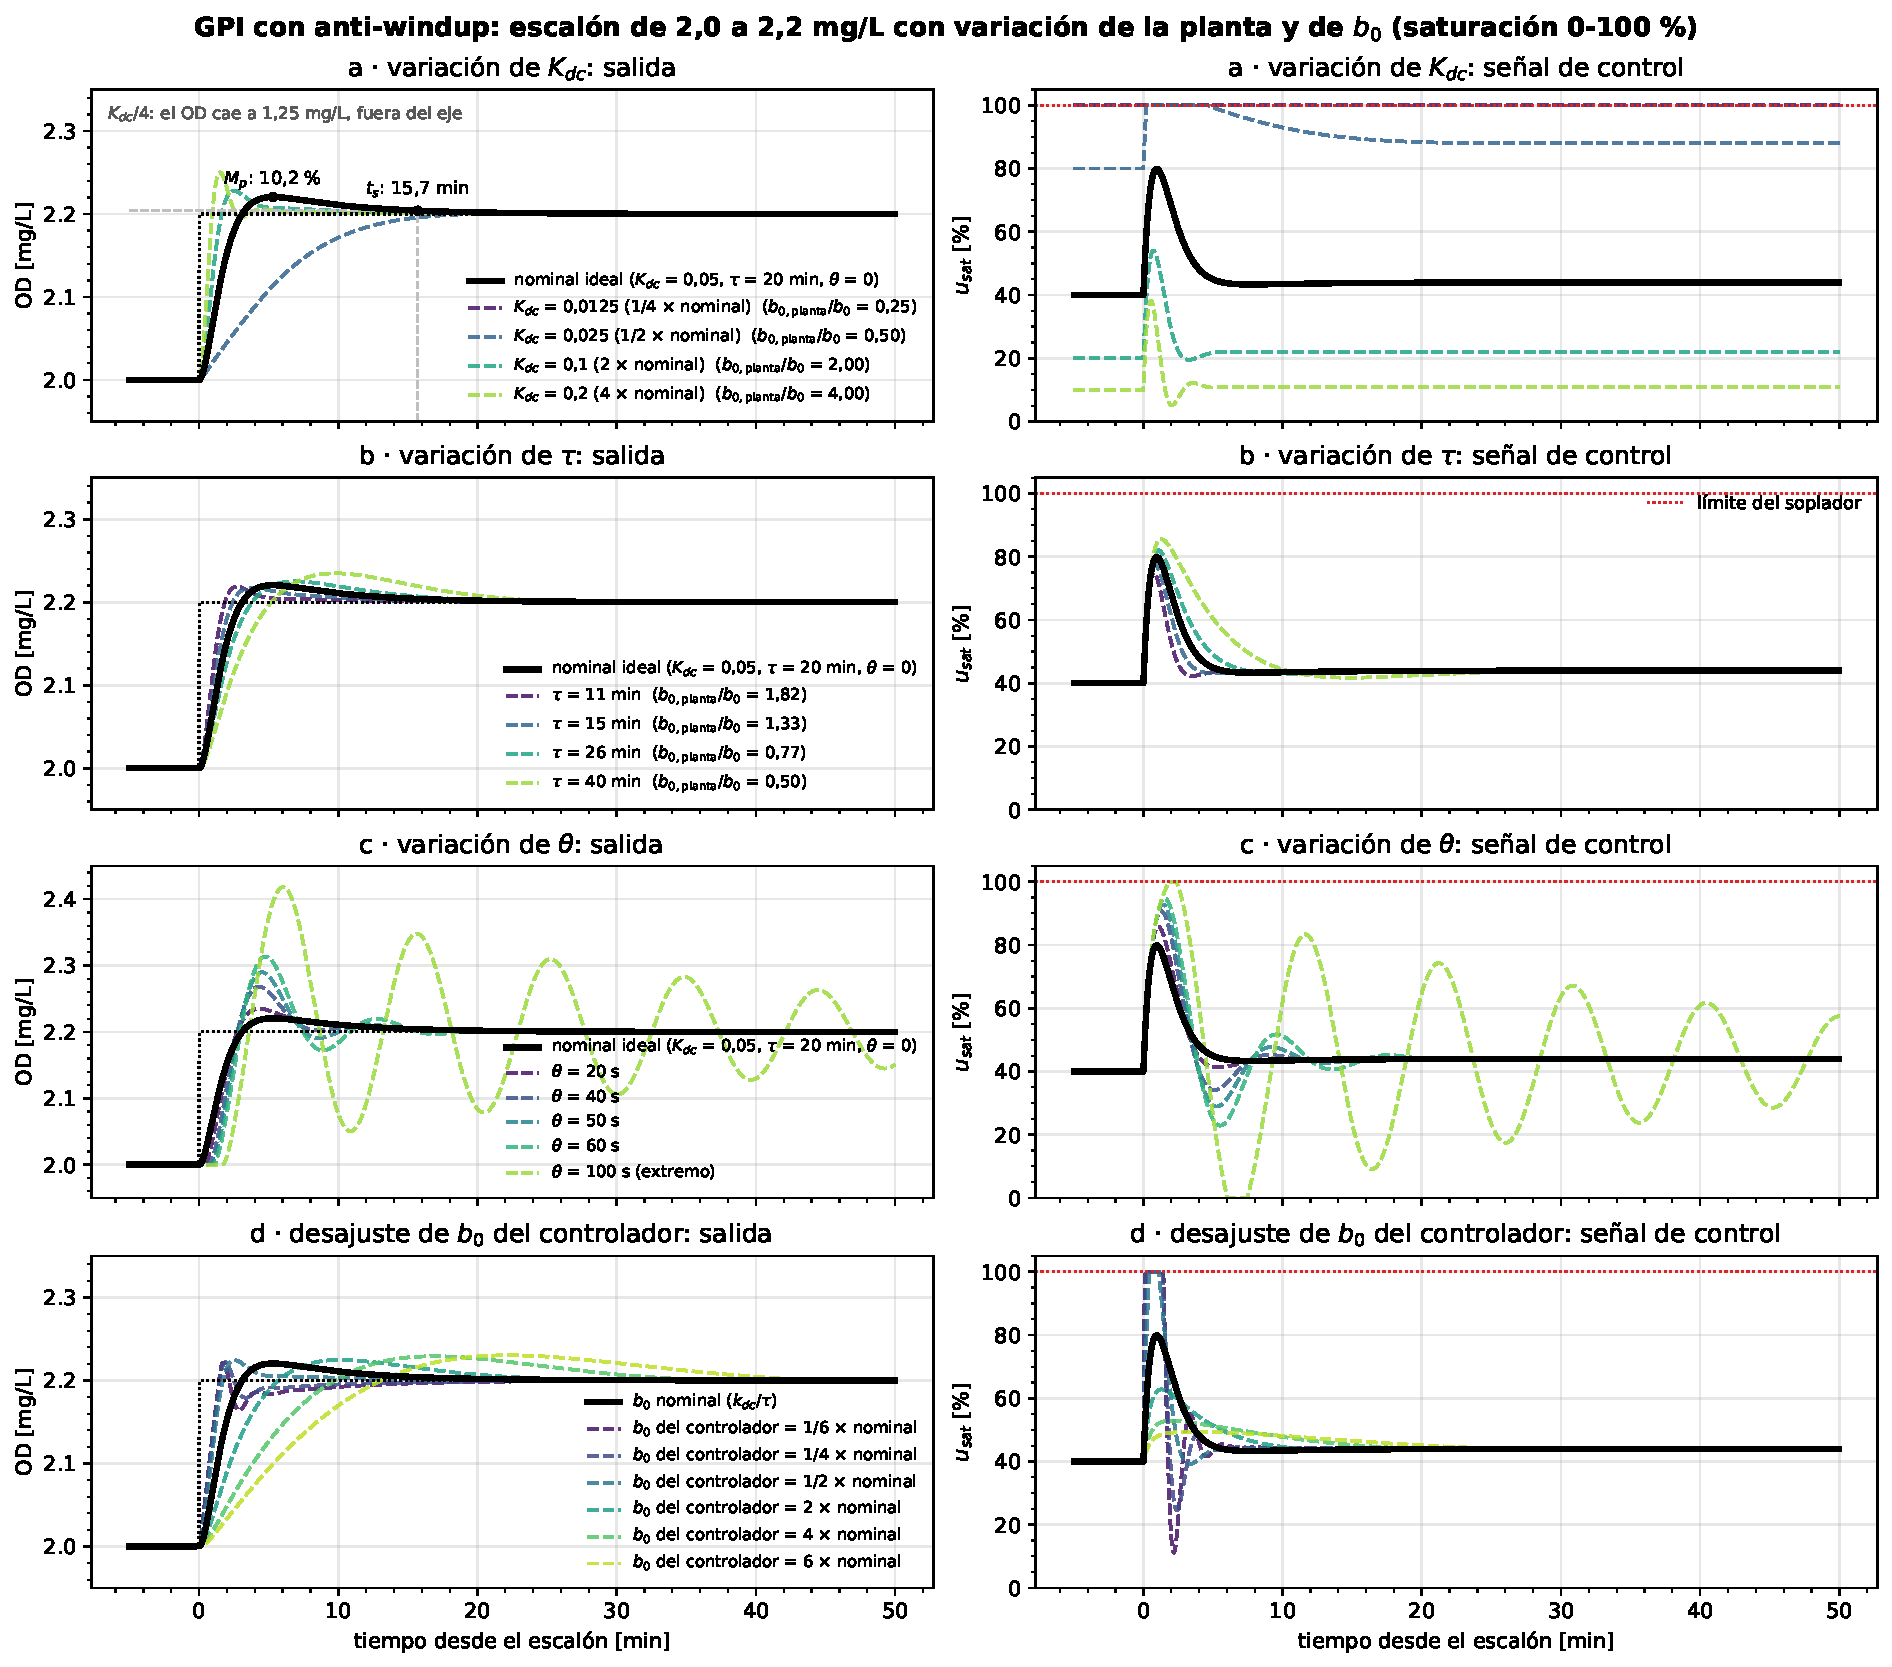
\includegraphics[width=\textwidth]{saturacion_adrc_gpi_variacion.pdf}
  \caption[GPI con saturación ante variaciones de la planta]{Escalón de
    consigna de $2{,}0$ a $2{,}2$~mg/L con el soplador limitado entre $0$ y
    $100~\%$ y el GPI con \emph{anti-windup} \eqref{eq:aw_gpi}, variando
    (a) $K_{dc}$, (b) $\tau$, (c) $\theta$, con un caso extremo de
    $\theta = 100$~s que satura el soplador, y (d) el $b_0$ del controlador. En
    negro, la planta nominal ideal, con $M_p$ y $t_s$ como en la Tabla~\ref{tab:metricas}.}
  \label{fig:sat_adrc_gpi_variacion}
\end{figure}



%--------------------------------------------------------------------
\section{Acondicionamiento de la referencia}
\label{sec:impl_referencia}

Ante un cambio de consigna, el ADRC basado en el error se pasa de la consigna aunque todos sus
polos sean reales (Sección~\ref{subsec:caso_variacion}). En el modelo de diseño (la cadena de
integradores), la respuesta a la consigna es
\begin{equation}
\frac{y}{r} = \frac{k_1 s + k_0}{s^3 + k_2 s^2 + k_1 s + k_0}
= \frac{k_1 s + k_0}{(s + \omega_c)\,(s + \omega_o)^2} .
\label{eq:pref_yr}
\end{equation}
Tiene tres polos, $-\omega_c$ (el del controlador) y $-\omega_o$ doble (el del observador), y un
cero en
\begin{equation}
s = -\frac{k_0}{k_1} = -\frac{\omega_c\,\omega_o}{\omega_o + 2\omega_c} = -\frac{5}{7}\,\omega_c ,
\end{equation}
más lento que el polo $-\omega_c$: ese cero es el que produce el sobrepico. Además, como se vio en
la Sección~\ref{subsec:caso_simulacion}, un escalón en la consigna pide un pico muy grande en la
señal de control, porque el controlador debe compensar $u^* = \dot{y}^*$, que es un impulso.

Las dos cosas se reducen acondicionando la referencia antes de que entre al lazo, de dos formas:
suavizándola con un polinomio de Bézier (Sección~\ref{subsec:impl_bezier}) o pasándola por un
prefiltro de primer orden (Sección~\ref{sec:impl_esfuerzo}). En ambos casos el controlador no cambia
y el rechazo de la perturbación sigue siendo el mismo.

%--------------------------------------------------------------------
\subsection{Polinomio de Bézier}
\label{subsec:impl_bezier}
Se presenta el esquema de la Figura~\ref{fig:lazo_bezier}, donde se muestra un
acondicionamiento previo de la señal de referencia: la entrada es suavizada por un
polinomio de Bézier, que se busca que inicie lento, es decir, con derivadas en cero,
y que termine lento, también con derivadas en cero.

\begin{figure}[H]
  \centering
  \begin{tikzpicture}[>=Stealth, thick, font=\small,
      blk/.style={draw, thick, minimum width=1.5cm, minimum height=0.9cm},
      suma/.style={draw, thick, circle, minimum size=0.45cm, inner sep=0pt}]
    % bloque de Bezier con la curva en S
    \node[blk, minimum width=1.7cm, minimum height=1.2cm] (bz) at (2.1,0) {};
    \draw[thin, gray, ->] ($(bz.center)+(-0.65,-0.42)$) -- ($(bz.center)+(0.68,-0.42)$);
    \draw[thin, gray, ->] ($(bz.center)+(-0.65,-0.42)$) -- ($(bz.center)+(-0.65,0.48)$);
    \draw[line width=1.1pt, domain=0:1, samples=40, variable=\x]
      plot ({-0.55+1.1*\x+2.1}, {-0.32+0.65*\x*\x*(3-2*\x)});
    \node[above=1pt of bz, font=\footnotesize] {Bézier};
    \node[suma] (sa) at (5.3,0) {};
    \node[blk] (Ca) at (8.0,0) {$C(s)$};
    \node[suma] (sb) at (10.1,0) {};
    \node[blk] (Ga) at (12.2,0) {$G(s)$};
    \draw[->] (0,0) node[above right] {$r(t)$} -- (bz.west);
    \draw[->] (bz.east) -- node[above, pos=0.4] {$y^*(t)$} (sa.west);
    \draw[->] (sa.east) -- node[above] {$-e_y(t)$} (Ca.west);
    \draw[->] (Ca.east) -- node[above] {$u(t)$} (sb.west);
    \draw[->] (sb |- 0,1.2) node[above] {$\varepsilon(t)$} -- (sb.north);
    \draw[->] (sb.east) -- (Ga.west);
    \node at ($(sb.west)+(-0.2,-0.25)$) {$+$};
    \node at ($(sb.north)+(0.25,0.2)$) {$+$};
    \draw[->] (Ga.east) -- (15.2,0) node[above left] {$y(t)$};
    \fill (14.5,0) circle (1.5pt);
    \draw[->] (14.5,0) -- (14.5,-1.2) -- (5.3,-1.2) -- (sa.south);
    \node at ($(sa.west)+(-0.2,0.25)$) {$+$};
    \node at ($(sa.south)+(-0.25,-0.2)$) {$-$};
  \end{tikzpicture}
  \caption[Lazo con acondicionamiento de la referencia]{Lazo de control por
    realimentación del error con acondicionamiento de la referencia: la
    consigna $r(t)$ pasa por el polinomio de Bézier y el lazo sigue $y^*(t)$,
    con $e_y = y - y^*$.}
  \label{fig:lazo_bezier}
\end{figure}

%--------------------------------------------------------------------
\subsubsection{Planificación de la referencia}
\label{subsec:bz_planificacion}
Ahora bien, para esto, la referencia lleva la salida desde $y_0$ hasta la consigna $y_f$, partiendo y
llegando en reposo. Como la planta es de primer orden, basta con que $y^*$ y
$\dot{y}^*$ sean continuas: dos condiciones en cada extremo y un polinomio de
grado 3,
\begin{equation}
\begin{aligned}
y^*(t) &= a_3 t^3 + a_2 t^2 + a_1 t + a_0 , \\
\dot{y}^*(t) &= 3a_3 t^2 + 2a_2 t + a_1 .
\end{aligned}
\label{eq:bz_pol}
\end{equation}
Evaluando en $t_0$ y $t_f$,
\begin{equation}
\underbrace{\begin{bmatrix} y^*(t_0) \\ \dot{y}^*(t_0) \\ y^*(t_f) \\ \dot{y}^*(t_f) \end{bmatrix}}_{\mathbf{y}_{t_0,t_f}}
=
\underbrace{\begin{bmatrix}
t_0^3 & t_0^2 & t_0 & 1 \\
3t_0^2 & 2t_0 & 1 & 0 \\
t_f^3 & t_f^2 & t_f & 1 \\
3t_f^2 & 2t_f & 1 & 0
\end{bmatrix}}_{\mathbf{A}_y}
\underbrace{\begin{bmatrix} a_3 \\ a_2 \\ a_1 \\ a_0 \end{bmatrix}}_{\mathbf{a}_y} ,
\qquad
\mathbf{y}_{t_0,t_f} = \begin{bmatrix} y_0 & 0 & y_f & 0 \end{bmatrix}^{\top} ,
\qquad
\mathbf{a}_y = \mathbf{A}_y^{-1}\,\mathbf{y}_{t_0,t_f} .
\label{eq:bz_sistema}
\end{equation}
Con $t_0 = 0$ y $\Delta = y_f - y_0$,
\begin{equation}
a_0 = y_0 , \qquad a_1 = 0 , \qquad a_2 = \frac{3\,\Delta}{t_f^2} , \qquad a_3 = -\frac{2\,\Delta}{t_f^3} ,
\label{eq:bz_cerrada}
\end{equation}
y con el tiempo normalizado $\tau = t/t_f \in [0, 1]$,
\begin{equation}
\left.
\begin{aligned}
y^*(t) &= y_0 + \Delta\,\tau^2\,(3 - 2\tau) , \\
\dot{y}^*(t) &= \frac{\Delta}{t_f}\,6\,\tau\,(1 - \tau) ,
\end{aligned}
\right\}
\qquad 0 \le t \le t_f ,
\label{eq:bz_normalizada}
\end{equation}
con $y^* = y_0$ para $t < t_0$ y $y^* = y_f$ para $t > t_f$. Es el polinomio de
Bézier de grado 3 con puntos de control $\{y_0,\, y_0,\, y_f,\, y_f\}$, y su
velocidad máxima, en $\tau = 1/2$, es
\begin{equation}
\dot{y}^*_{\max} = 1{,}5\,\frac{\Delta}{t_f} .
\label{eq:bz_vmax}
\end{equation}
Las ecuaciones \eqref{eq:bz_normalizada} son las que se programan dentro de un bloque
de PLC: solo es necesario obtener la normalización del tiempo $\tau$ y medir el
tiempo actual, que se obtienen fácilmente con un contador y el tiempo de muestreo.
%--------------------------------------------------------------------
\subsubsection{Cambio de consigna y replanificación}
\label{subsec:bz_replanificacion}
Seguidamente se plantea el caso en que el operario realiza un cambio de consigna
cuando el sistema va subiendo.
Si la consigna cambia en $t_c$, el nuevo tramo parte del estado de la referencia,
no de la medición, con $t_0 = 0$ y $\tau = (t - t_c)/t_f$:
\begin{equation}
y_c = y^*(t_c) , \qquad \dot{y}_c = \dot{y}^*(t_c) , \qquad \bar{\Delta} = y_f - y_c ,
\label{eq:bz_estado_c}
\end{equation}
\begin{equation}
\begin{bmatrix} y_c \\ \dot{y}_c \\ y_f \\ 0 \end{bmatrix}
=
\begin{bmatrix}
0 & 0 & 0 & 1 \\
0 & 0 & 1 & 0 \\
t_f^3 & t_f^2 & t_f & 1 \\
3t_f^2 & 2t_f & 1 & 0
\end{bmatrix}
\begin{bmatrix} a_3 \\ a_2 \\ a_1 \\ a_0 \end{bmatrix}
\quad\Longrightarrow\quad
\begin{aligned}
a_0 &= y_c , & a_1 &= \dot{y}_c , \\
a_2 &= \frac{3\bar{\Delta} - 2\,\dot{y}_c\,t_f}{t_f^2} , & a_3 &= \frac{-2\bar{\Delta} + \dot{y}_c\,t_f}{t_f^3} .
\end{aligned}
\label{eq:bz_sistema_c}
\end{equation}
Con $c_i = a_i\,t_f^{\,i}$,
\begin{equation}
c_1 = \dot{y}_c\,t_f , \qquad
c_2 = 3\bar{\Delta} - 2\,\dot{y}_c\,t_f , \qquad
c_3 = -2\bar{\Delta} + \dot{y}_c\,t_f ,
\label{eq:bz_c}
\end{equation}
y de forma compacta:
\begin{equation}
\left.
\begin{aligned}
y^*(\tau) &= y_c + \tau\,\bigl(c_1 + \tau\,(c_2 + \tau\,c_3)\bigr) , \\
\dot{y}^*(\tau) &= \frac{1}{t_f}\,\bigl(c_1 + \tau\,(2c_2 + 3\tau\,c_3)\bigr) ,
\end{aligned}
\right\}
\qquad 0 \le \tau \le 1 ,
\label{eq:bz_horner}
\end{equation}
con $y^* = y_f$ y $\dot{y}^* = 0$ para $\tau > 1$. Con $\dot{y}_c = 0$,
\eqref{eq:bz_c} da $c_1 = 0$, $c_2 = 3\bar{\Delta}$ y $c_3 = -2\bar{\Delta}$, que es
\eqref{eq:bz_cerrada}. En el PLC, $\tau = n\,T_s/t_f$, con $n$ los ciclos desde
el inicio del tramo; al cambiar la consigna se recalcula \eqref{eq:bz_c} y se
reinicia $n = 0$, y al salir de \texttt{RESET} se toma $y_c = y$ medido y
$\dot{y}_c = 0$.

%--------------------------------------------------------------------
\subsubsection{Simulación en lazo cerrado}
\label{subsec:bz_simulacion}
La Figura~\ref{fig:adrc_lazo_cerrado_bezier} muestra el comportamiento de la planta cuando
se usa una referencia más suave, como la de Bézier. En el panel (a), el transitorio de $0$ a
$2{,}0$~mg/L dura unos $48$~min (cerca de $2{,}4\,\tau$), el tiempo final elegido para esa
maniobra, y el cambio de consigna de $2{,}0$ a $2{,}2$~mg/L se hace con un tiempo final de
$1\,\tau$. Como el suavizado solo se aplica a la referencia, el rechazo de la perturbación
exógena es prácticamente igual. En el panel (b) se puede observar que el observador logra
estimar adecuadamente el error de seguimiento (por ser de alta ganancia), aunque no de forma
exacta, por lo que sí se
sigue la curva de Bézier a pesar de que el modelo interno no tiene ese polinomio. Finalmente,
la señal de control se mantiene por debajo del $62~\%$ (panel d), por lo que sí se ve
reflejada una disminución muy buena de la señal de control.

Ahora bien, la Figura~\ref{fig:adrc_bezier_retardo} muestra el comportamiento de la planta
cuando se involucran retardos. Sin el acondicionamiento de la referencia (panel a), el
sobrepico va aumentando a medida que crece $\theta$; pero cuando se usa Bézier (panel b),
las oscilaciones prácticamente desaparecen, y aunque haya retardo, la planta logra un
transitorio suave, sin oscilaciones grandes que puedan llegar a saturar el controlador.

\begin{figure}[H]
  \centering
  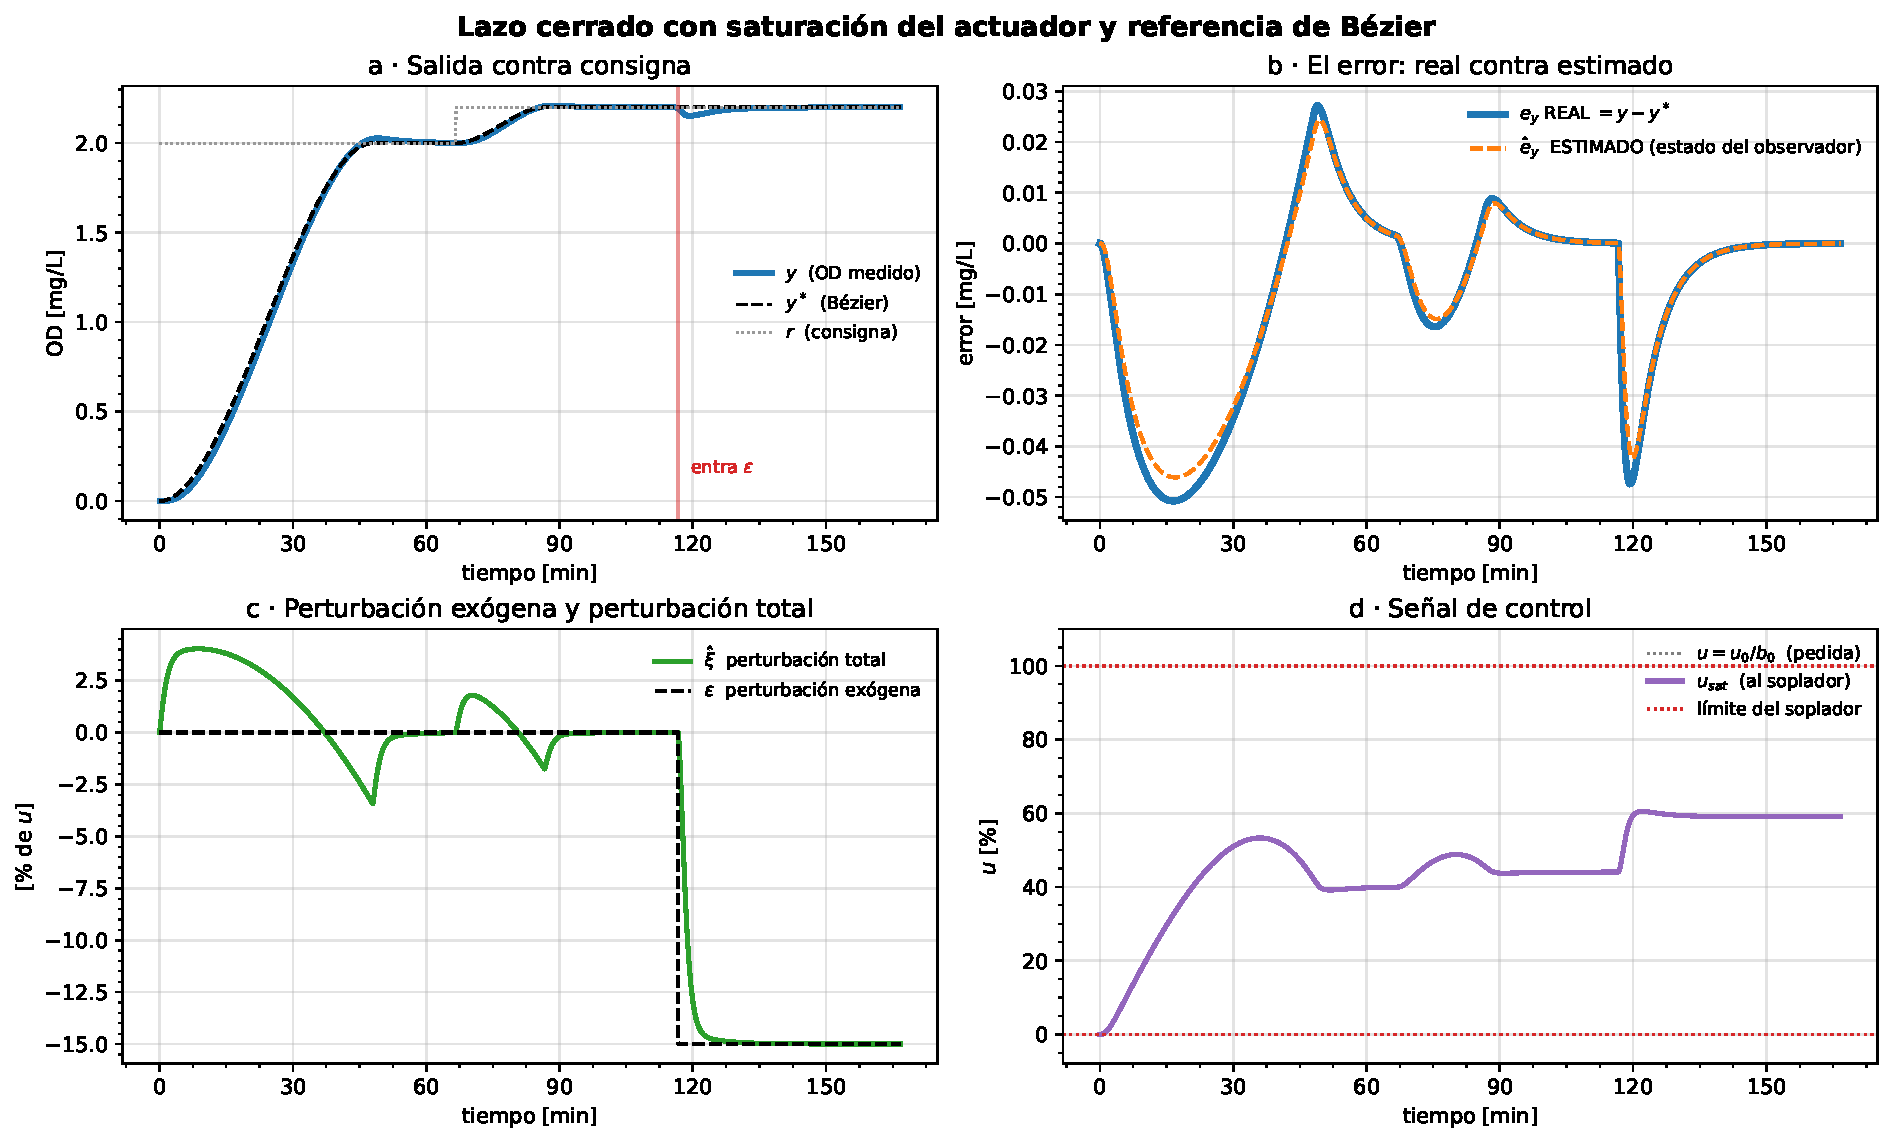
\includegraphics[width=\textwidth]{adrc_lazo_cerrado_bezier.pdf}
  \caption[Lazo cerrado del ADRC con referencia de Bézier]{Lazo cerrado del
    ADRC con la planta, el soplador limitado entre $0$ y $100~\%$ y la
    referencia de Bézier \eqref{eq:bz_normalizada}, en el mismo escenario de la
    Figura~\ref{fig:adrc_lazo_cerrado_saturacion}. (a) Salida contra la
    referencia $y^*$ y la consigna $r$. (b) Error de seguimiento real y
    estimado. (c) Perturbación exógena y perturbación total, en \% de $u$.
    (d) Orden pedida por el controlador y orden aplicada.}
  \label{fig:adrc_lazo_cerrado_bezier}
\end{figure}

\begin{figure}[H]
  \centering
  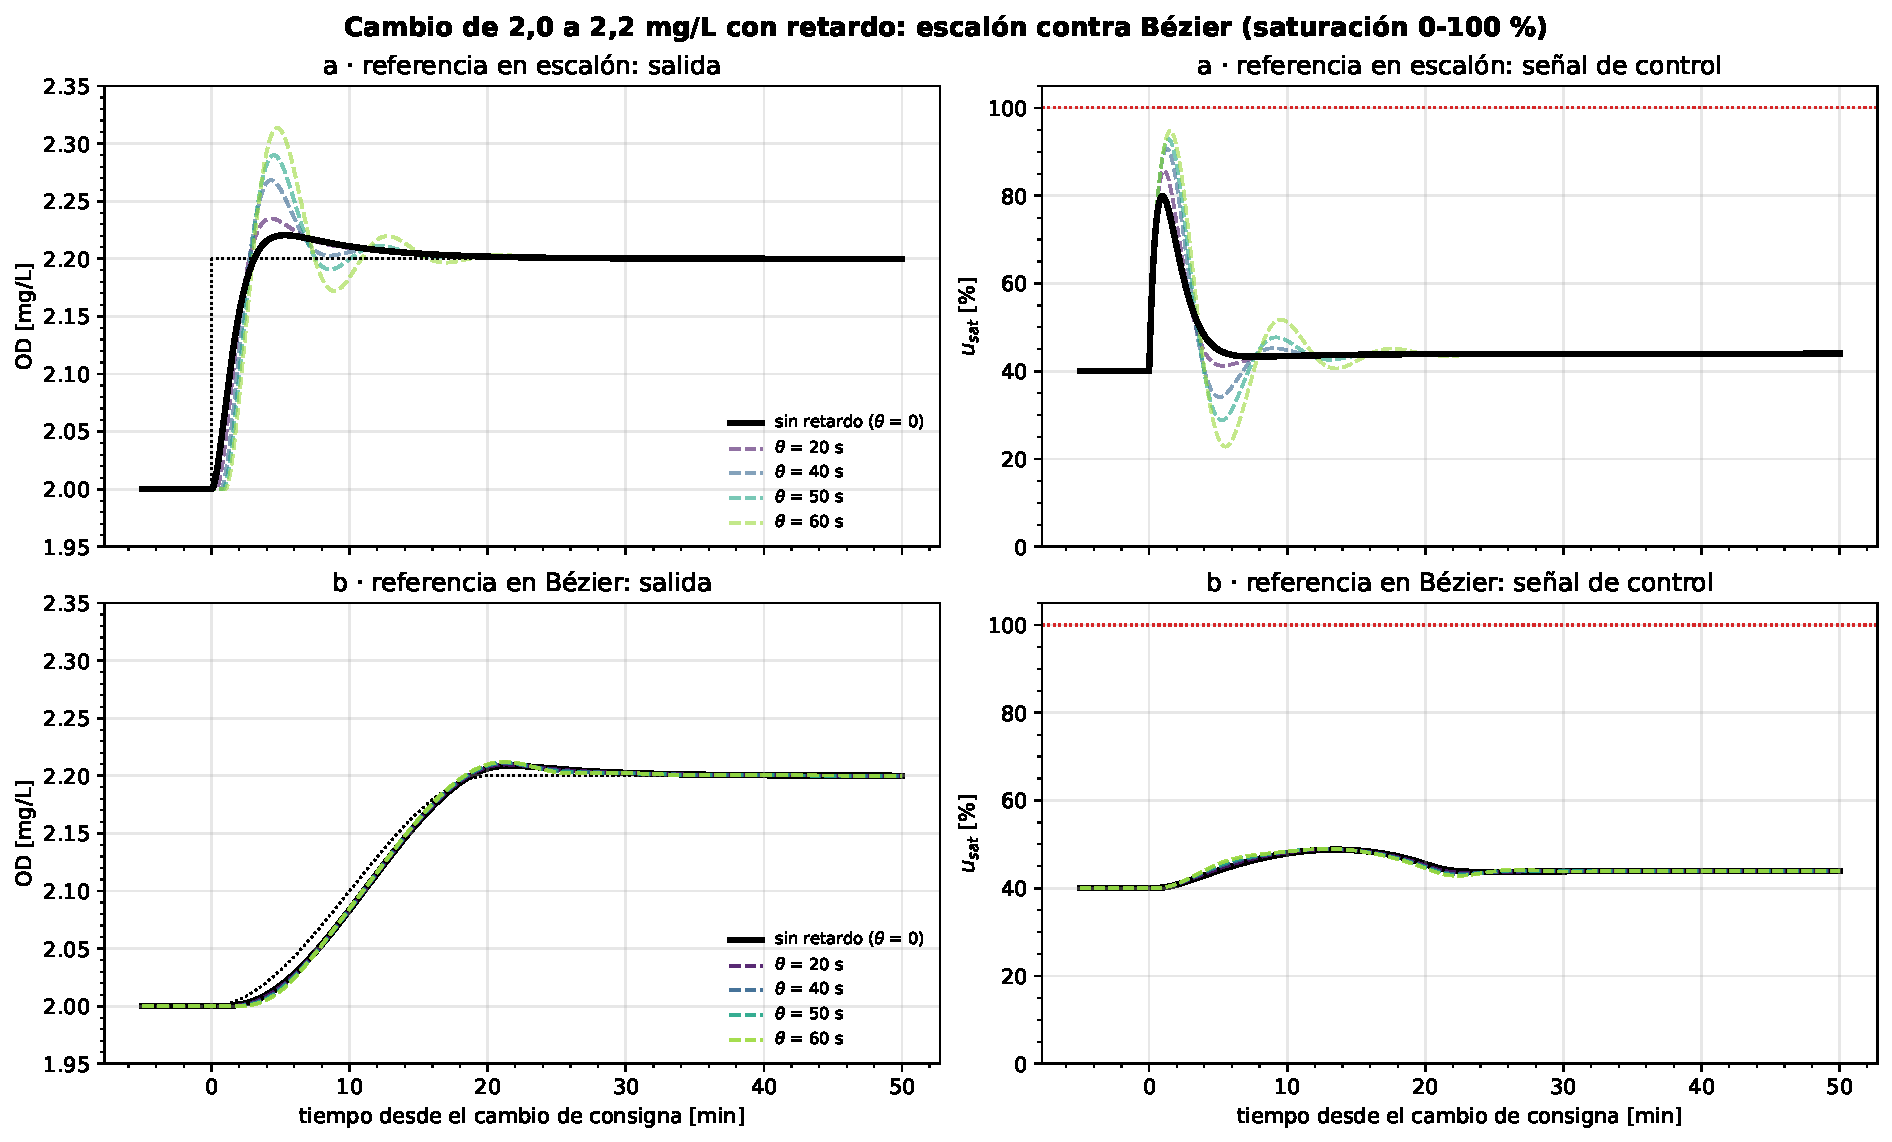
\includegraphics[width=\textwidth]{adrc_bezier_retardo.pdf}
  \caption[Escalón contra Bézier con retardo]{Cambio de consigna de $2{,}0$ a
    $2{,}2$~mg/L con la planta nominal, retardo $\theta$ en la entrada y el
    soplador limitado entre $0$ y $100~\%$: (a) consigna en escalón y
    (b) referencia de Bézier con $t_f = 20$~min. En negro, sin retardo.}
  \label{fig:adrc_bezier_retardo}
\end{figure}


%--------------------------------------------------------------------
\subsection{Prefiltro de consigna}
\label{sec:impl_esfuerzo}

Herbst y Madoński proponen agregar un prefiltro en el canal de la referencia del ADRC basado en
el error \cite[sec.~6.4.2]{herbst2024adrc}. Para quitar el cero de \eqref{eq:pref_yr}, aquí se pone
antes de la suma un prefiltro de primer orden con el polo justo en ese cero
(Figura~\ref{fig:pref_lazo}):
\begin{equation}
F(s) = \frac{k_0}{k_1 s + k_0} = \frac{1}{\dfrac{k_1}{k_0}\,s + 1}
= \frac{1}{\dfrac{\omega_o + 2\omega_c}{\omega_c\,\omega_o}\,s + 1} ,
\label{eq:pref_f}
\end{equation}
con ganancia estática $1$, para que la salida llegue a la consigna, y constante de tiempo
$k_1/k_0 = 420$~s ($7$~min). El prefiltro está fuera del lazo: el controlador no cambia y le sigue
entrando solo el error, ahora $e_y = y - r_f$.

\begin{figure}[H]
  \centering
  \begin{tikzpicture}[>=Stealth, thick, font=\small,
      blk/.style={draw, thick, minimum width=1.5cm, minimum height=0.9cm},
      suma/.style={draw, thick, circle, minimum size=0.45cm, inner sep=0pt}]
    \node[blk, minimum width=2.2cm, minimum height=1.1cm] (pf) at (2.2,0) {$\dfrac{k_0}{k_1 s + k_0}$};
    \node[above=1pt of pf, font=\footnotesize] {prefiltro};
    \node[suma] (sa) at (5.5,0) {};
    \node[blk] (Ca) at (8.0,0) {$C(s)$};
    \node[suma] (sb) at (10.5,0) {};
    \node[blk] (Ga) at (12.6,0) {$G(s)$};
    \draw[->] (0,0) node[above right] {$r(t)$} -- (pf.west);
    \draw[->] (pf.east) -- node[above] {$r_f(t)$} (sa.west);
    \draw[->] (sa.east) -- node[above] {$-e_y(t)$} (Ca.west);
    \draw[->] (Ca.east) -- node[above] {$u(t)$} (sb.west);
    \draw[->] (sb |- 0,1.2) node[above] {$\varepsilon(t)$} -- (sb.north);
    \draw[->] (sb.east) -- node[above] {$\bar{u}(t)$} (Ga.west);
    \draw[->] (Ga.east) -- (15.1,0) node[above left] {$y(t)$};
    \fill (14.4,0) circle (1.5pt);
    \draw[->] (14.4,0) -- (14.4,-1.2) -- (5.5,-1.2) -- (sa.south);
    \node at ($(sa.west)+(-0.2,0.25)$) {$+$};
    \node at ($(sa.south)+(-0.25,-0.2)$) {$-$};
    \node at ($(sb.west)+(-0.2,0.25)$) {$+$};
    \node at ($(sb.north)+(0.25,0.2)$) {$+$};
  \end{tikzpicture}
  \caption[Lazo con prefiltro de consigna]{Lazo de control con prefiltro de consigna, con
    $e_y = y - r_f$. El prefiltro está fuera del lazo.}
  \label{fig:pref_lazo}
\end{figure}

Con el prefiltro, el polo se cancela con el cero en \eqref{eq:pref_yr} y quedan los tres polos del
diseño, sin cero:
\begin{equation}
\begin{aligned}
\frac{y}{r} &= \frac{k_0}{k_1 s + k_0}\cdot\frac{k_1 s + k_0}{s^3 + k_2 s^2 + k_1 s + k_0} \\[4pt]
&= \frac{k_0}{s^3 + k_2 s^2 + k_1 s + k_0} = \frac{k_0}{(s + \omega_c)\,(s + \omega_o)^2} .
\end{aligned}
\label{eq:pref_yr_f}
\end{equation}
La respuesta a la perturbación no pasa por el prefiltro, así que sigue siendo la misma. En el
modelo de diseño, la perturbación total $\bar{\xi}$ entra a la cadena de integradores junto con $u_0$, y
\begin{equation}
\frac{y}{\bar{\xi}} = \frac{s\,(s + k_2)}{s^3 + k_2 s^2 + k_1 s + k_0}
= \frac{s\,(s + k_2)}{(s + \omega_c)\,(s + \omega_o)^2} ,
\label{eq:pref_rechazo}
\end{equation}
que no tiene ese cero y no cambia con $F(s)$. Es decir, el filtro solo se ve en el seguimiento de
la referencia y no en el rechazo de la perturbación.

En el escalón de $2{,}0$ a $2{,}2$~mg/L con la planta (Figura~\ref{fig:pref_escalon}), sin
retardo el prefiltro quita el sobrepico ($10{,}3$ a $0~\%$), baja el pico de $u$ de $80$ a $50~\%$
y la energía de la señal de control $E_u$ (Tabla~\ref{tab:metricas}) de $2132$ a $203~\%^2\cdot$min. Con
$\theta = 50$~s el sobrepico baja de $46$ a $0~\%$, el pico de $u$ de $93$ a $54~\%$ y $E_u$ de $4844$ a
$320~\%^2\cdot$min. A
cambio llega más tarde: entra a la banda de $2~\%$ en $24{,}4$~min en vez de $15{,}7$ sin retardo, y
en $24{,}7$ en vez de $14{,}7$ con $\theta = 50$~s. La perturbación de $-15~\%$ da la misma caída con
y sin prefiltro: el oxígeno baja hasta $2{,}15$~mg/L sin retardo y hasta $2{,}13$~mg/L con
$\theta = 50$~s.

\begin{figure}[H]
  \centering
  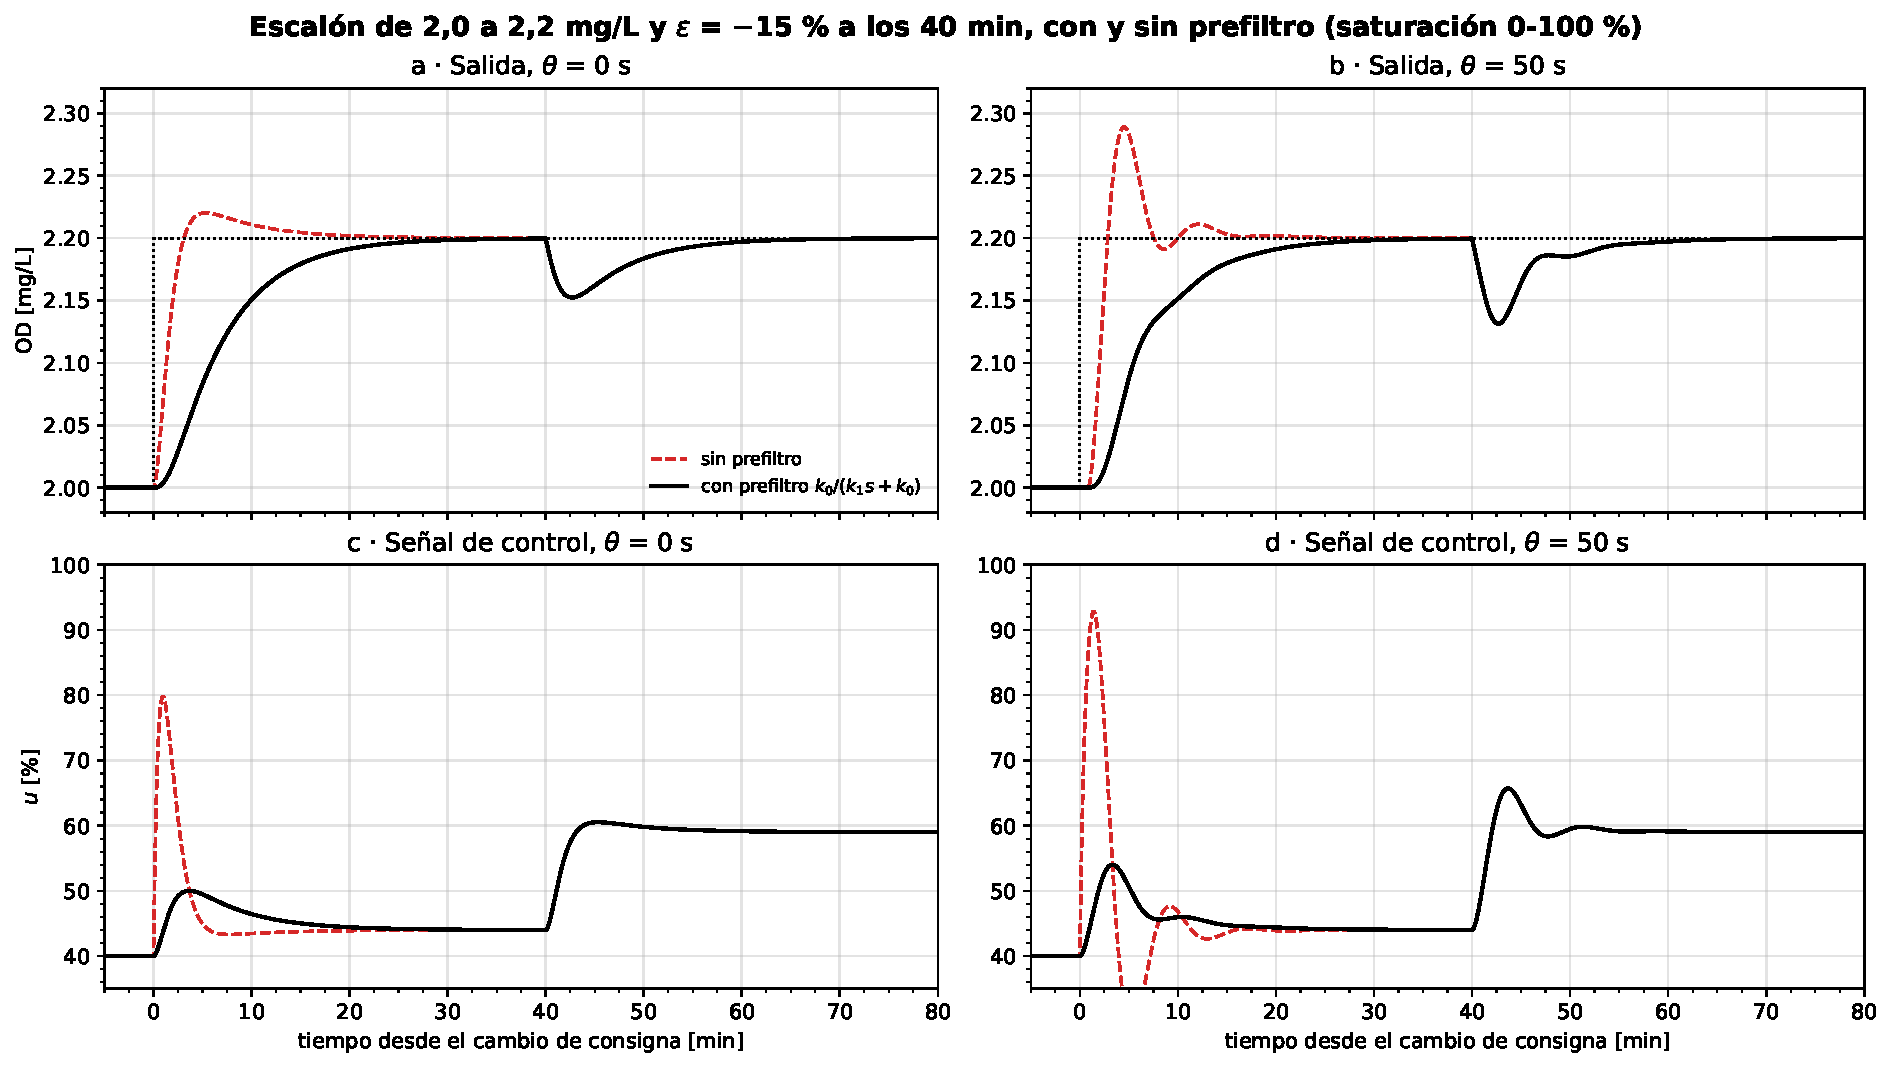
\includegraphics[width=\textwidth]{adrc_prefiltro.pdf}
  \caption[Escalón de consigna y perturbación con y sin prefiltro]{Escalón de consigna de
    $2{,}0$ a $2{,}2$~mg/L y perturbación $\varepsilon = -15~\%$ a los $40$~min, con la planta
    y el soplador limitado entre $0$ y $100~\%$, sin prefiltro y con el prefiltro
    \eqref{eq:pref_f}. (a) y (c) Sin retardo; (b) y (d) con $\theta = 50$~s. Arriba, la salida;
    abajo, la señal de control.}
  \label{fig:pref_escalon}
\end{figure}
Si se llega a cambiar la estructura del controlador, para seguir otro tipo de referencias, como
una rampa, o por el orden de la planta, es necesario reajustar el filtro según la estructura del
controlador, para anular los ceros del numerador de $y/r$. No es una regla exacta: poniendo un
filtro libre se pueden obtener buenos resultados suavizando la referencia, como en el ejemplo de
Herbst y Madoński \cite[sec.~6.4.2]{herbst2024adrc}; pero si se quiere la dinámica exacta del
diseño, sí es necesario reajustar el filtro con polos que cancelen los ceros del lazo cerrado.

%--------------------------------------------------------------------
\section{Manejo del ruido}
\label{sec:impl_ruido}

Chen clasifica las funciones de transferencia según lo que hacen en alta frecuencia, y eso es lo que
decide cómo tratan el ruido. Una función de transferencia es estrictamente propia si $G(\infty) = 0$,
bipropia si $G(\infty)$ es finito y distinto de cero, e impropia si
$G(\infty) = \infty$ \cite[sec.~2.4]{chen1993analog}. Las impropias amplifican
el ruido de alta frecuencia, como un derivador, y las estrictamente propias lo
atenúan, como un integrador \cite[pp.~31--32]{chen1993analog}; por eso todo
compensador debe ser al menos propio \cite[sec.~6.5]{chen1993analog}.

El ruido $n$ de la medida llega al error y al soplador por las funciones de transferencia de la
Tabla~\ref{tab:caso_gang}:
\begin{equation}
\frac{-e_y}{n} = \frac{-1}{1 + CG},
\qquad
\frac{u}{n} = \frac{-C}{1 + CG} .
\label{eq:ruido_ft}
\end{equation}
Por encima del ancho de banda, con $C$ bipropio el
ruido pasa al soplador con la ganancia $C(\infty)$ hasta la frecuencia de
Nyquist; con $C$ estrictamente propio, se atenúa.

El GPI \eqref{eq:gpi_pi_filtro} es estrictamente propio: su ganancia cae como
$1/\omega$ y tiende a cero,
\begin{equation}
C_{GPI}(s) = \frac{1}{b_0}\,\frac{k_1 s + k_0}{s\,(s + k_2)},
\qquad
|C_{GPI}(j\omega)| \xrightarrow{\;\omega \to \infty\;} \frac{k_1}{b_0\,\omega} \to 0,
\qquad
C_{GPI}(\infty) = 0 .
\end{equation}
Sin el filtro, con su
ganancia estática $1/k_2$, queda el PI bipropio clásico, cuya ganancia tiende a
una constante:
\begin{equation}
C_{PI}(s) = \frac{1}{b_0 k_2}\,\frac{k_1 s + k_0}{s},
\qquad
C_{PI}(\infty) = \frac{k_1}{b_0 k_2} = 254{,}5~\%/(\mathrm{mg/L}) .
\end{equation}
El ruido en el error llega casi el mismo con los dos controladores, pero en $u$ el PI se queda en
$48{,}1$~dB hasta Nyquist y el GPI cae $20$~dB/década
(Figura~\ref{fig:ruido_gpi_vs_pi}). Simulados con el ruido del sensor
(Sección~\ref{sec:ident_ruido}), $\sigma_u$ da $0{,}0080~\%$ con el GPI y
$0{,}28~\%$ con el PI, $35$ veces más: el PI deja pasar mucho más ruido a la señal de control. En
el escalón del
Capítulo~\ref{cap:comparacion_pid} pasa lo mismo con el PID ISA, también
bipropio: $0{,}22~\%$ frente a $0{,}009~\%$ del ADRC
(Figura~\ref{fig:pid_adrc_escalon},
Tabla~\ref{tab:pid_escalon}).

\begin{figure}[H]
  \centering
  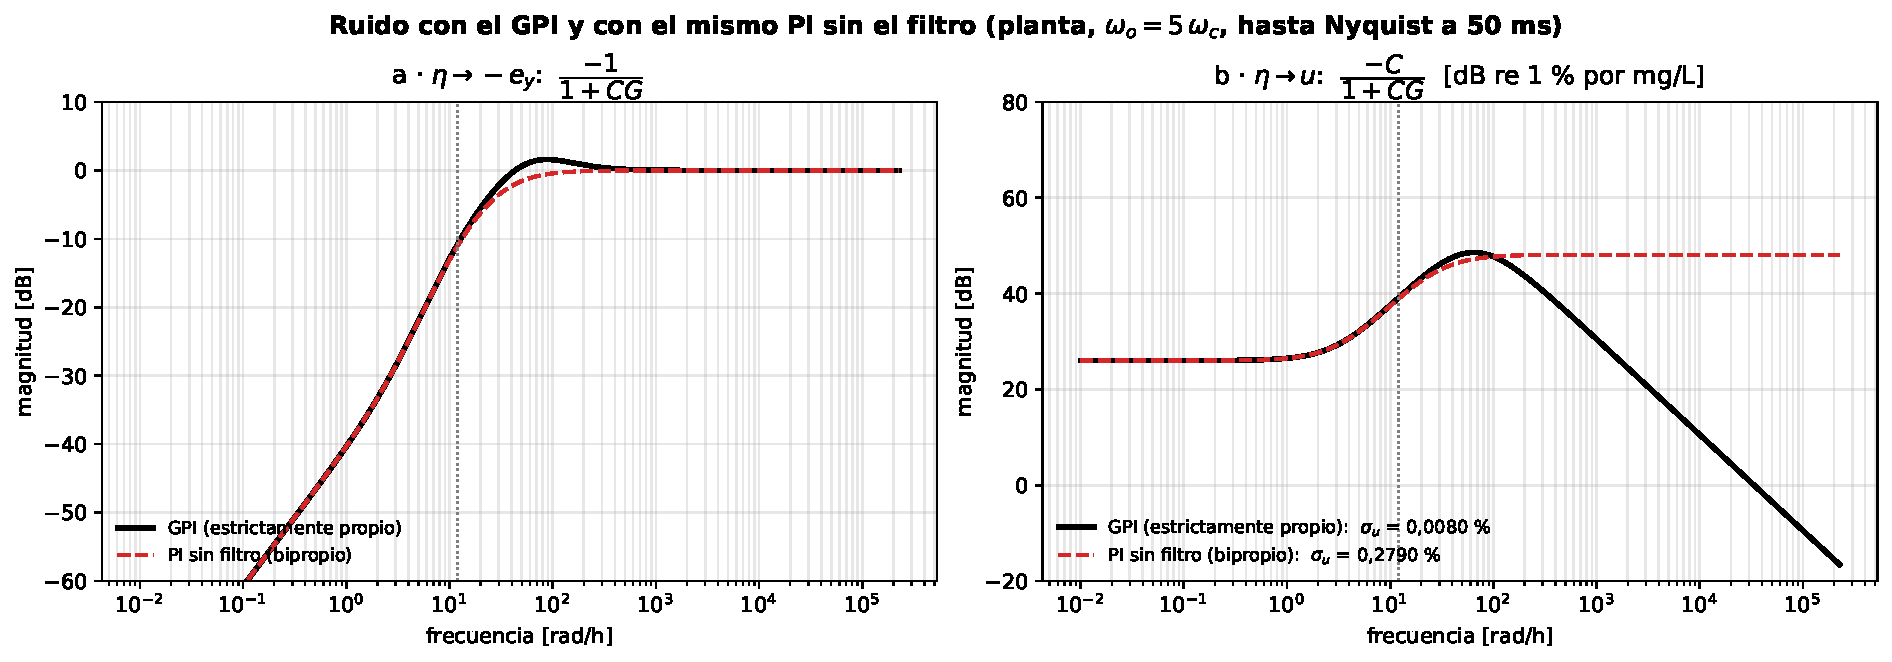
\includegraphics[width=\textwidth]{ruido_gpi_vs_pi.pdf}
  \caption[Ruido con el GPI y con el PI sin filtro]{Funciones de transferencia
    del ruido \eqref{eq:ruido_ft} con la planta y $\omega_o = 5\,\omega_c$,
    hasta la frecuencia de Nyquist a $50$~ms: GPI (estrictamente propio) y el
    mismo PI sin el filtro (bipropio). (a) Hacia $-e_y$. (b) Hacia $u$, con la
    $\sigma_u$ simulada con el ruido del sensor. La vertical marca $\omega_c$.}
  \label{fig:ruido_gpi_vs_pi}
\end{figure}

Herbst y Madoński presentan la misma idea: el controlador del ADRC, que es el mismo en el enfoque
basado en el error, es estrictamente propio \cite[ecs.~4.20 y 6.30]{herbst2024adrc}, y el máximo de
$\omega_o$ lo pone el ruido admisible en $u$
\cite[secs.~5.3.3 y 9.3]{herbst2024adrc}. Es decir, al pasar de $\omega_o = 5\,\omega_c$ a
$10\,\omega_c$, el ruido llega al soplador con $3{,}4$ veces más ganancia
(Figura~\ref{fig:adrc_gang_kESO}(h)). Con $\omega_o = 5\,\omega_c$ y un
controlador estrictamente propio no hacen falta filtros adicionales. Por ende, con el ADRC, ya sea basado en
observador de estado extendido o en su forma GPI, se puede ajustar el ruido admisible con el ancho de banda
del observador, $\omega_o$. Queda entonces la anotación de que el ajuste de $\omega_o$ dependerá de
las frecuencias de las perturbaciones que se desean rechazar y del tope máximo de ruido admisible
que se deja pasar a la señal de control.

%--------------------------------------------------------------------
\section{Discretización}
\label{sec:impl_discretizacion}

En el PLC el controlador es un sistema digital: el error se muestrea con un
conversor A/D, el controlador discreto $C(z)$ calcula la orden en cada periodo de
muestreo $T_s$, y un conversor D/A la mantiene constante hasta la muestra
siguiente (Figura~\ref{fig:lazo_digital}) \cite[sec.~12.1]{chen1993analog}.

\begin{figure}[H]
  \centering
  \begin{tikzpicture}[>=Stealth, thick, font=\small,
      blk/.style={draw, thick, minimum width=1.3cm, minimum height=0.9cm},
      suma/.style={draw, thick, circle, minimum size=0.45cm, inner sep=0pt}]
    \node[suma] (sa) at (1.6,0) {};
    \node[blk] (ad) at (3.9,0) {A/D};
    \node[blk, minimum width=1.6cm] (cz) at (6.5,0) {$C(z)$};
    \node[blk] (da) at (9.1,0) {D/A};
    \node[blk, minimum width=1.6cm] (gs) at (11.7,0) {$G(s)$};
    \node[blk, minimum width=1.5cm, minimum height=0.6cm] (ck) at (6.5,-1.05) {reloj};
    \draw[->] (0,0) node[above right] {$r(t)$} -- (sa.west);
    \draw[->] (sa.east) -- node[above] {$-e_y(t)$} (ad.west);
    \draw[->] (ad.east) -- node[above] {$-e_y[k]$} (cz.west);
    \draw[->] (cz.east) -- node[above] {$u[k]$} (da.west);
    \draw[->] (da.east) -- node[above] {$u(t)$} (gs.west);
    \draw[->] (gs.east) -- (14.4,0) node[above left] {$y(t)$};
    \fill (13.7,0) circle (1.5pt);
    \draw[->] (13.7,0) -- (13.7,-1.75) -- (1.6,-1.75) -- (sa.south);
    \draw[->] (ck.west) -- (ad |- ck) -- (ad.south);
    \draw[->] (ck.east) -- (da |- ck) -- (da.south);
    \draw[->] (ck.north) -- (cz.south);
    \node at ($(sa.west)+(-0.2,0.25)$) {$+$};
    \node at ($(sa.south)+(-0.25,-0.2)$) {$-$};
  \end{tikzpicture}
  \caption[Lazo de control digital]{Lazo de control digital, con
    $e_y = y - r$ \cite[fig.~12.1]{chen1993analog}.}
  \label{fig:lazo_digital}
\end{figure}

Las técnicas de realimentación de estado y de estimadores del caso continuo se
aplican sin modificaciones al discreto; la diferencia es que los polos deseados
se ubican dentro del círculo unitario \cite[sec.~13.7]{chen1993analog}.

\paragraph{Métodos de discretización.} El controlador continuo,
$C(s) = \frac{1}{b_0}\frac{k_1 s + k_0}{s\,(s + k_2)}$, se puede llevar a $C(z)$ con
\begin{equation}
\begin{gathered}
\text{ZOH: } C(z) = (1 - z^{-1})\,\mathcal{Z}\!\left\{\frac{C(s)}{s}\right\},
\qquad
\text{Tustin: } s \to \frac{2}{T_s}\,\frac{z - 1}{z + 1},\\[4pt]
\text{Euler hacia adelante: } s \to \frac{z - 1}{T_s},
\qquad
\text{Euler hacia atrás: } s \to \frac{z - 1}{T_s\,z},
\end{gathered}
\label{eq:disc_metodos}
\end{equation}
o diseñarse directamente en discreto (Sección~\ref{subsec:disc_adrc}). La
Figura~\ref{fig:disc_metodos_bode} compara sus respuestas en frecuencia,
evaluadas en $z = e^{j\omega T_s}$ hasta la frecuencia de Nyquist, $\pi/T_s$.

\begin{figure}[H]
  \centering
  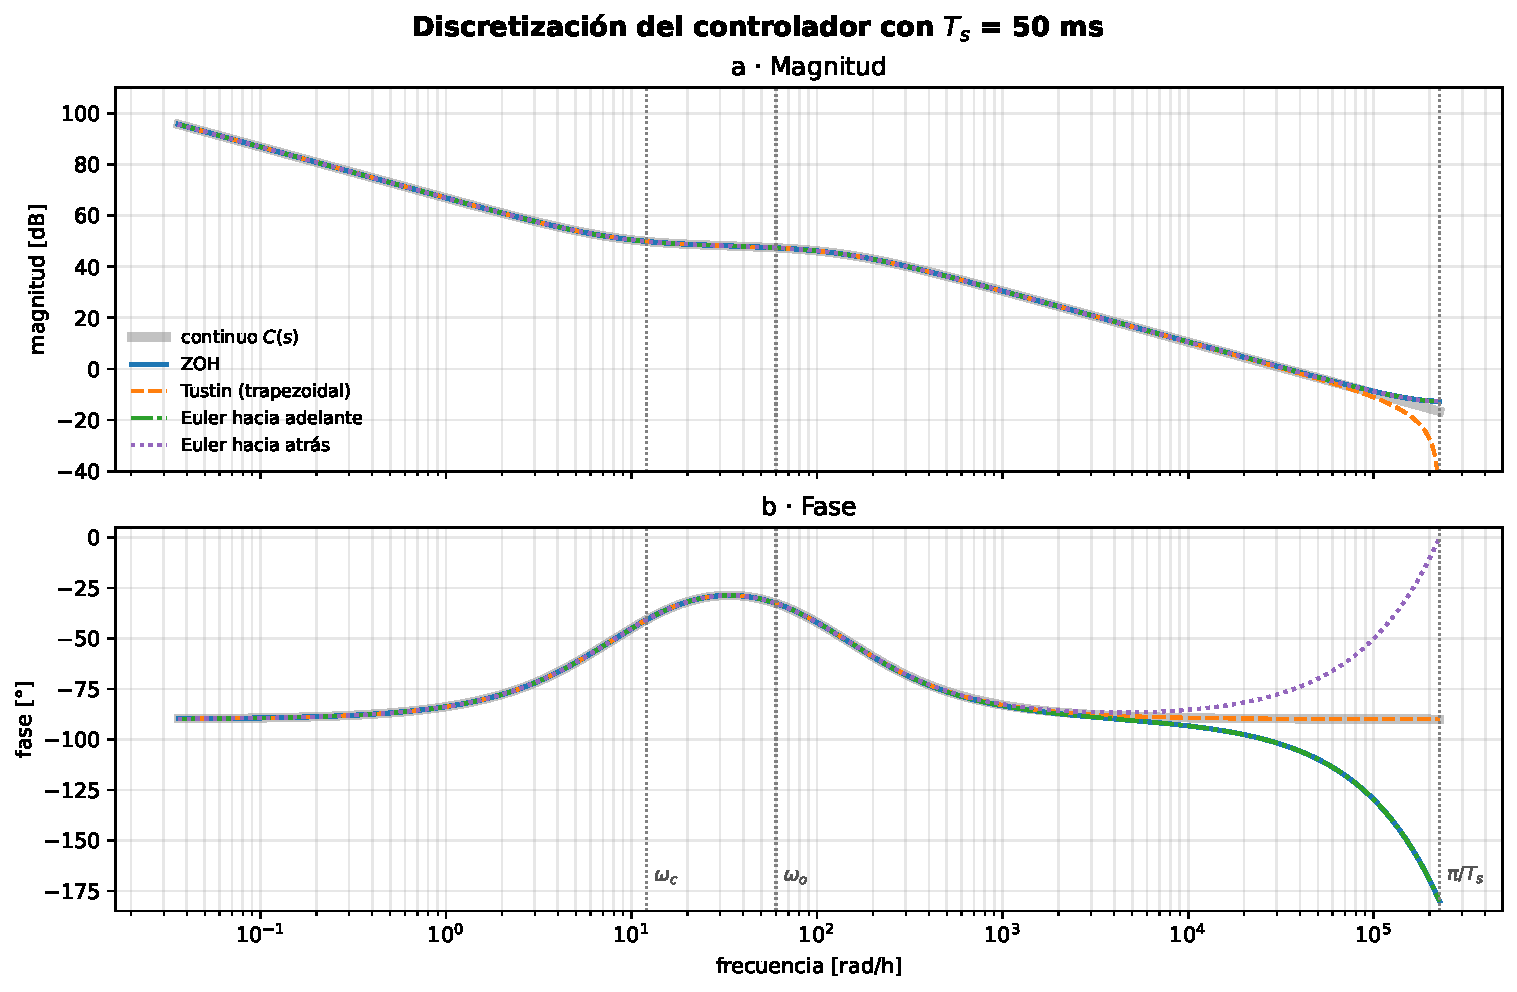
\includegraphics[width=0.85\textwidth]{disc_metodos_bode.pdf}
  \caption[Discretización del controlador por distintos métodos]{Respuesta en
    frecuencia del controlador continuo $C(s)$ y de sus versiones discretas con
    $T_s = 50$~ms: ZOH, Tustin, Euler hacia adelante y Euler hacia atrás.
    (a) Magnitud y (b) fase; las verticales
    marcan $\omega_c$, $\omega_o$ y la frecuencia de Nyquist $\pi/T_s$.}
  \label{fig:disc_metodos_bode}
\end{figure}

En la Figura~\ref{fig:disc_metodos_bode} se observa que, hasta unos
$10^4$~rad/h, todas las curvas prácticamente coinciden con la del controlador
continuo, y que las frecuencias $\omega_o$ y $\omega_c$ se encuentran alejadas
en más de dos décadas de ese valor. Por lo tanto, en este caso se obtiene un buen
resultado sin importar el método de discretización que se use. Esto se debe
directamente al tiempo de muestreo, ya que la planta es muy lenta comparada con
él. Chen menciona que el muestreo debe ser, como mínimo, unas 10 veces el ancho
de banda del lazo cerrado, recomienda unas 20 veces, y concluye que, si el periodo
es suficientemente pequeño, cualquier método sirve para discretizar un
compensador analógico
\cite[sec.~13.3.1]{chen1993analog}. El ancho de banda del lazo cerrado con la planta es de
$56{,}4$~rad/h, y la frecuencia de muestreo,
$\omega_s = 2\pi/T_s = 125{,}7$~rad/s, es decir,
$4{,}52\times10^{5}$~rad/h, queda casi cuatro órdenes de magnitud por encima. Si
se muestreara a 10 veces el ancho de banda del lazo cerrado, se tendría
$\omega_s = 564$~rad/h, es decir, un tiempo de muestreo de $40$~s; con este
valor de $T_s$ se obtiene la Figura~\ref{fig:disc_metodos_bode_40}. Se observa
que, en las frecuencias del lazo de control, las magnitudes se mantienen juntas,
mientras que en la fase algunos métodos empiezan a separarse del continuo. El
método que mantuvo un comportamiento más parecido al continuo, en magnitud y en
fase, a la frecuencia del lazo cerrado es Tustin.

\begin{figure}[H]
  \centering
  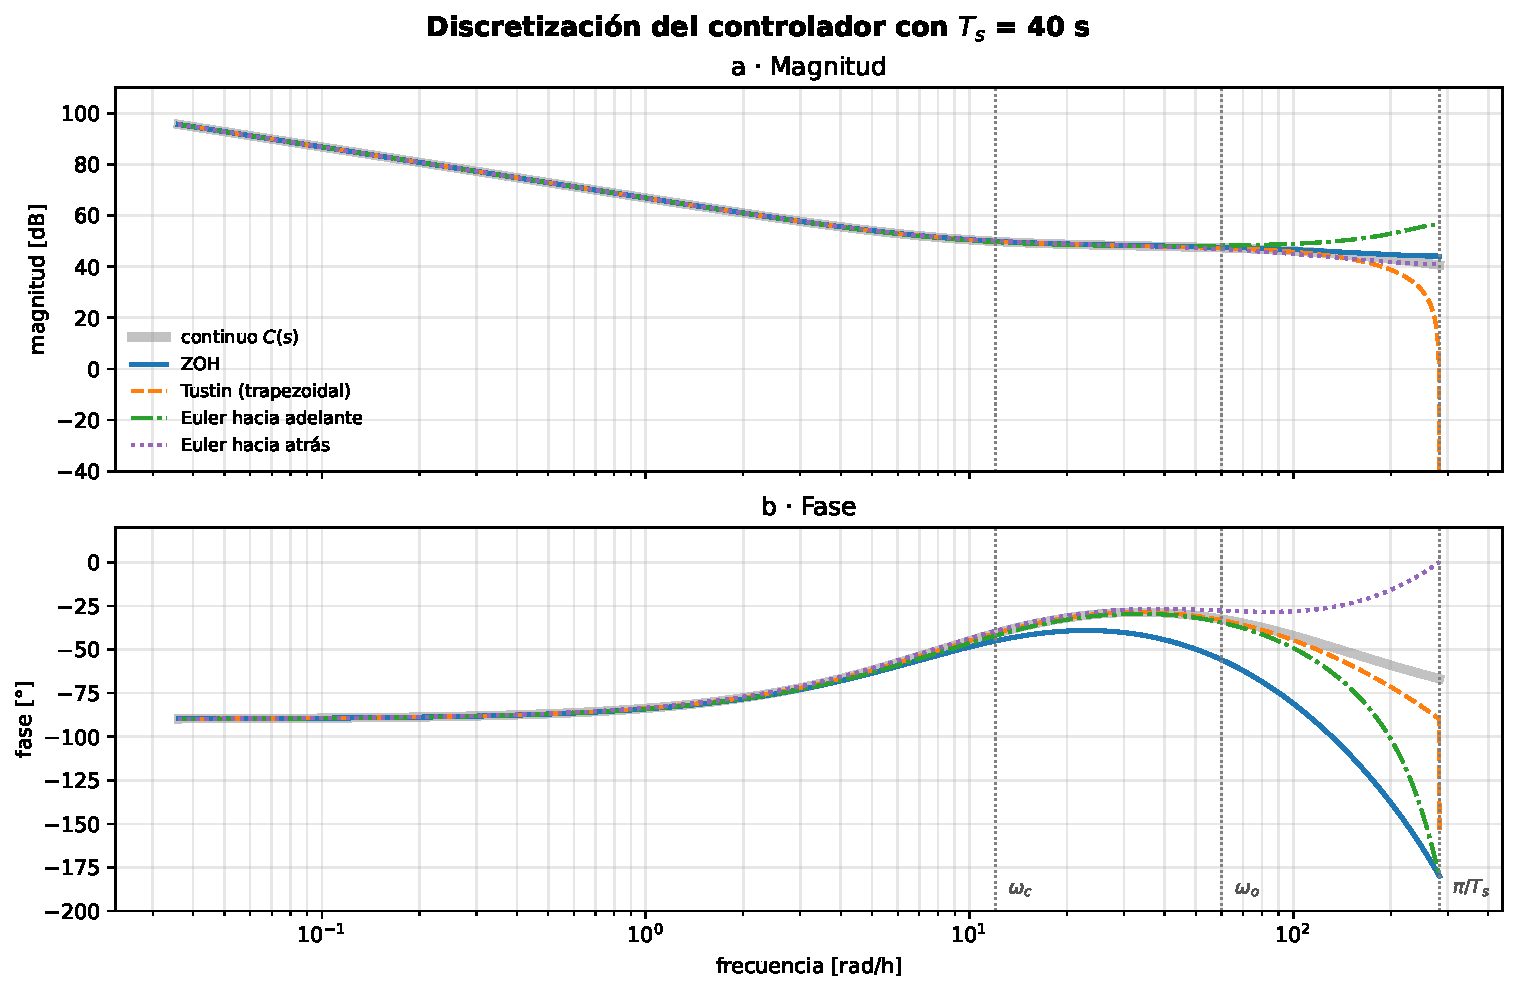
\includegraphics[width=0.85\textwidth]{disc_metodos_bode_40s.pdf}
  \caption[Discretización del controlador con $T_s = 40$~s]{Respuesta en
    frecuencia del controlador continuo $C(s)$ y de sus versiones discretas con
    $T_s = 40$~s, 10 veces el ancho de banda del lazo cerrado: ZOH, Tustin,
    Euler hacia adelante y Euler hacia atrás. (a) Magnitud y (b) fase; las
    verticales marcan $\omega_c$,
    $\omega_o$ y la frecuencia de Nyquist $\pi/T_s$.}
  \label{fig:disc_metodos_bode_40}
\end{figure}

%--------------------------------------------------------------------
\subsection{ADRC basado en observador de estado}
\label{subsec:disc_adrc}

El controlador se ejecuta cada $T_s = 50$~ms: el conversor A/D muestrea el
error y el conversor D/A mantiene la orden aplicada constante entre muestras,
como un retenedor de orden cero (ZOH). El modelo de diseño se discretiza con el
mismo retenedor (Figura~\ref{fig:adrc_discreto}).

\begin{figure}[H]
  \centering
  \resizebox{\textwidth}{!}{%
  \begin{tikzpicture}[>=Stealth, thick, font=\small,
      blk/.style={draw, thick, minimum width=1.3cm, minimum height=0.9cm},
      suma/.style={draw, thick, circle, minimum size=0.45cm, inner sep=0pt}]
    \node[suma] (sa) at (3.2,0) {};

    % --- ADRC discreto: observador, ley de control y saturacion ---
    \node[block, minimum width=6.0cm, minimum height=1.9cm] (obs) at (8.9,-0.4)
      {$\mathbf{A}_o\widehat{\mathbf{X}}[k] + \mathbf{B}_o \mathbf{u}_t[k]$ \\[10pt]
       $\mathbf{C}_o\widehat{\mathbf{X}}[k] + \mathbf{D}_o \mathbf{u}_t[k]$};
    \node[above=2pt of obs] {Observador discreto};
    \node[block, minimum size=9mm] (K) at (13.8,0) {$-\mathbf{K}_d$};
    \coordinate (u0) at (15.3,0);
    \node[block, minimum size=9mm] (ib) at (16.7,0) {$1/b_0$};
    \node[block, minimum size=11mm] (sat) at (19.0,0) {};
    \draw[thin, gray] ($(sat.center)+(-0.38,0)$) -- ($(sat.center)+(0.38,0)$);
    \draw[thin, gray] ($(sat.center)+(0,-0.38)$) -- ($(sat.center)+(0,0.38)$);
    \draw[line width=1.1pt] ($(sat.center)+(-0.38,-0.22)$) -- ($(sat.center)+(-0.18,-0.22)$)
                         -- ($(sat.center)+(0.18,0.22)$) -- ($(sat.center)+(0.38,0.22)$);
    \node[above=2pt of sat, font=\footnotesize] {0--100~\%};
    \coordinate (us) at (20.5,0);
    \node[block, minimum size=9mm] (gb) at (13.8,-2.1) {$b_0$};
    \draw[red, dashed, thick] (5.35,1.8) rectangle (21.0,-2.9);
    \node[below right] at (5.35,1.8) {ADRC discreto};

    % --- planta discreta ---
    \node[suma] (sb) at (22.6,0) {};
    \node[block, align=center, minimum width=4.4cm, minimum height=1.9cm] (gs) at (26.5,0)
      {$\mathbf{A}_{g,d}\,\mathbf{x}_g[k] + \mathbf{B}_{g,d}\,\bar{u}[k]$ \\[10pt]
       $\mathbf{C}_{g,d}\,\mathbf{x}_g[k] + \mathbf{D}_{g,d}\,\bar{u}[k]$};
    \node[above=2pt of gs] {Planta discreta};

    % --- señales ---
    \draw[->] (1.4,0) node[above right] {$r[k]$} -- (sa.west);
    \draw[->] (sa.east) -- node[above, pos=0.35] {$e_y[k]$} (obs.west |- 0,0);
    \draw[->] (obs.east |- K) -- node[above] {$\widehat{\mathbf{X}}[k]$} (K.west);
    \draw (K.east) -- (u0) node[above] {$u_0[k]$};
    \draw[->] (u0) -- (ib.west);
    \draw[->] (ib.east) -- node[above] {$u[k]$} (sat.west);
    \draw (sat.east) -- (us);
    \fill (us) circle (1.5pt);
    \draw[->] (us) -- node[above, pos=0.55] {$u_{\mathrm{sat}}[k]$} (sb.west);
    \draw[->] (us) -- (us |- 0,-2.1) -- (gb.east);
    \draw[->] (gb.west) -- (5.62,-2.1) node[above right] {$b_0\,u_{\mathrm{sat}}[k]$}
              -- (5.62,-0.85) -- (obs.west |- 0,-0.85);
    \draw[->] (sb |- 0,1.5) node[above] {$\varepsilon[k]$} -- (sb.north);
    \draw[->] (sb.east) -- node[above, pos=0.5] {$\bar{u}[k]$} (gs.west);
    \draw[->] (gs.east) -- (30.0,0) node[above left] {$y[k]$};
    \fill (29.3,0) circle (1.5pt);
    \draw[->] (29.3,0) -- (29.3,-3.5) -- (3.2,-3.5) -- (sa.south);
    \node at ($(sa.west)+(-0.2,0.25)$) {$-$};
    \node at ($(sa.south)+(-0.25,-0.2)$) {$+$};
    \node at ($(sb.west)+(-0.2,-0.25)$) {$+$};
    \node at ($(sb.north)+(-0.25,0.2)$) {$+$};
  \end{tikzpicture}%
  }
  \caption[ADRC discreto con saturación]{Lazo discreto con el ADRC discreto y
    la planta discretizada (Tabla~\ref{tab:disc_matrices}). El observador y la
    ley de control con saturación se evalúan en el instante $k$, y al
    observador se le realimenta la orden aplicada $b_0\,u_{\mathrm{sat}}[k]$. El
    observador tiene una estructura predictiva \cite[sec.~8.1.1]{herbst2024adrc}: con la
    medida del instante $k$ estima el estado en $k+1$.}
  \label{fig:adrc_discreto}
\end{figure}

\paragraph{Sistema aumentado discreto.} El sistema aumentado
\eqref{eq:aumentado} se arma con la planta de diseño y el modelo interno. Para
pasarlo a discreto, cada parte se discretiza por separado con la discretización
de \cite[sec.~4.2.1]{chen1999linear}, $\mathbf{A}_d = e^{\mathbf{A}T_s}$ y
$\mathbf{B}_d = \int_0^{T_s} e^{\mathbf{A}t}\,dt\;\mathbf{B}$, con $\gamma_i = 0$.

\textit{Planta de diseño} (cadena de $n$ integradores):
\begin{equation}
\begin{gathered}
\mathbf{A}_p =
\begin{bmatrix} 0 & 1 & \cdots & 0 \\ \vdots & \ddots & \ddots & \vdots \\ 0 & \cdots & 0 & 1 \\ 0 & \cdots & 0 & 0 \end{bmatrix}_{n \times n},
\qquad
\mathbf{B}_p = \begin{bmatrix} 0 \\ \vdots \\ 0 \\ 1 \end{bmatrix}_{n \times 1},
\qquad
\mathbf{C}_p = \begin{bmatrix} 1 & 0 & \cdots & 0 \end{bmatrix}_{1 \times n},
\\[8pt]
\mathbf{A}_{p,d} = e^{\mathbf{A}_p T_s} =
\begin{bmatrix} 1 & T_s & \cdots & \frac{T_s^{n-1}}{(n-1)!} \\ \vdots & \ddots & \ddots & \vdots \\ 0 & \cdots & 1 & T_s \\ 0 & \cdots & 0 & 1 \end{bmatrix},
\quad
\mathbf{B}_{p,d} = \int_0^{T_s} e^{\mathbf{A}_p t}\,dt\;\mathbf{B}_p =
\begin{bmatrix} \frac{T_s^{n}}{n!} \\ \vdots \\ \frac{T_s^{2}}{2!} \\ T_s \end{bmatrix},
\quad
\mathbf{C}_{p,d} = \mathbf{C}_p .
\end{gathered}
\label{eq:disc_planta}
\end{equation}

\textit{Modelo interno} (cadena de $m$ integradores):
\begin{equation}
\begin{gathered}
\mathbf{A}_{\xi} =
\begin{bmatrix} 0 & 1 & \cdots & 0 \\ \vdots & \ddots & \ddots & \vdots \\ 0 & \cdots & 0 & 1 \\ 0 & \cdots & 0 & 0 \end{bmatrix}_{m \times m},
\qquad
\mathbf{B}_{\xi} = \begin{bmatrix} 0 \\ \vdots \\ 0 \\ 1 \end{bmatrix}_{m \times 1},
\qquad
\mathbf{C}_{\xi} = \begin{bmatrix} 1 & 0 & \cdots & 0 \end{bmatrix}_{1 \times m},
\\[8pt]
\mathbf{A}_{\xi,d} = e^{\mathbf{A}_{\xi} T_s} =
\begin{bmatrix} 1 & T_s & \cdots & \frac{T_s^{m-1}}{(m-1)!} \\ \vdots & \ddots & \ddots & \vdots \\ 0 & \cdots & 1 & T_s \\ 0 & \cdots & 0 & 1 \end{bmatrix},
\quad
\mathbf{B}_{\xi,d} = \int_0^{T_s} e^{\mathbf{A}_{\xi} t}\,dt\;\mathbf{B}_{\xi} =
\begin{bmatrix} \frac{T_s^{m}}{m!} \\ \vdots \\ \frac{T_s^{2}}{2!} \\ T_s \end{bmatrix},
\quad
\mathbf{C}_{\xi,d} = \mathbf{C}_{\xi} .
\end{gathered}
\label{eq:disc_modelo}
\end{equation}

El sistema aumentado discreto se arma igual que en el continuo:
\begin{equation}
\begin{gathered}
\mathbf{A}_d =
\begin{bmatrix} \mathbf{A}_{p,d} & \mathbf{B}_{p,d}\,\mathbf{C}_{\xi} \\ \mathbf{0}_{m \times n} & \mathbf{A}_{\xi,d} \end{bmatrix},
\qquad
\mathbf{B}_d = \begin{bmatrix} \mathbf{B}_{p,d} \\ \mathbf{0}_{m \times 1} \end{bmatrix},
\qquad
\mathbf{E}_d = \begin{bmatrix} \mathbf{0}_{n \times 1} \\ \mathbf{B}_{\xi,d} \end{bmatrix},
\\[6pt]
\mathbf{C}_d = \mathbf{C}, \qquad \mathbf{D}_d = \mathbf{D} = 0 .
\end{gathered}
\label{eq:disc_armado}
\end{equation}
La discretización es exacta para $u_0$, dado que, al usar el D/A, se mantiene constante
entre muestras (retenedor de orden cero): entre dos muestras la planta acumula la integral
de lo que le entra, y como $u_0$ no cambia durante el periodo, sale de esa integral y queda
$\mathbf{B}_{p,d}\,u_0[k]$ sin ninguna aproximación. A $\xi$ se le da el mismo trato: se
supone constante durante cada periodo y entra a la planta por el mismo canal que $u_0$, a
través del bloque $\mathbf{B}_{p,d}\,\mathbf{C}_{\xi}$ de $\mathbf{A}_d$. Para $\xi$ esto ya
no es exacto, porque sí puede cambiar dentro del periodo; lo que el modelo interno no
alcanza a describir queda en el residuo $p_{\xi}[k]$, que entra al modelo interno por
$\mathbf{E}_d$ \eqref{eq:disc_separacion}. Este residuo es cero cuando $\xi$ sigue
exactamente el modelo interno elegido, por ejemplo, una $\xi$ constante con $m = 1$; en ese
caso, además, armar el sistema por partes da lo mismo que discretizar el sistema aumentado
completo, $\mathbf{A}_d = e^{\mathbf{A}T_s}$. Las matrices $\mathbf{C}$ y $\mathbf{D}$ no
cambian, y el sistema discreto queda:

\begin{recuadro}{Sistema aumentado discreto de orden $n+m$}
\begin{equation}
\begin{gathered}
\mathbf{X}[k+1] = \mathbf{A}_d\,\mathbf{X}[k] + \mathbf{B}_d\,u_0[k] + \mathbf{E}_d\,p_{\xi}[k],
\\[4pt]
e_y[k] = \mathbf{C}_d\,\mathbf{X}[k],
\qquad \mathbf{C}_d = \begin{bmatrix} 1 & 0 & \cdots & 0 \end{bmatrix},
\end{gathered}
\label{eq:disc_aumentado}
\end{equation}
\begin{equation}
\begin{gathered}
\mathbf{A}_d =
\left[\begin{array}{cccc|cccc}
1 & T_s & \cdots & \frac{T_s^{n-1}}{(n-1)!} & \frac{T_s^{n}}{n!} & 0 & \cdots & 0 \\
\vdots & \ddots & \ddots & \vdots & \vdots & \vdots & & \vdots \\
0 & \cdots & 1 & T_s & \frac{T_s^{2}}{2!} & 0 & \cdots & 0 \\
0 & \cdots & 0 & 1 & T_s & 0 & \cdots & 0 \\ \hline
0 & \cdots & 0 & 0 & 1 & T_s & \cdots & \frac{T_s^{m-1}}{(m-1)!} \\
\vdots & & \vdots & \vdots & \vdots & \ddots & \ddots & \vdots \\
0 & \cdots & 0 & 0 & 0 & \cdots & 1 & T_s \\
0 & \cdots & 0 & 0 & 0 & \cdots & 0 & 1
\end{array}\right],
\\[8pt]
\mathbf{B}_d =
\left[\begin{array}{c}
\frac{T_s^{n}}{n!} \\ \vdots \\ \frac{T_s^{2}}{2!} \\ T_s \\ \hline \mathbf{0}_{m \times 1}
\end{array}\right],
\qquad
\mathbf{E}_d =
\left[\begin{array}{c}
\mathbf{0}_{n \times 1} \\[2pt] \hline \frac{T_s^{m}}{m!} \rule{0pt}{3ex} \\ \vdots \\ \frac{T_s^{2}}{2!} \\ T_s
\end{array}\right] .
\end{gathered}
\label{eq:disc_matrices}
\end{equation}
Los bloques diagonales son $\mathbf{A}_{p,d}$ ($n \times n$) y
$\mathbf{A}_{\xi,d}$ ($m \times m$); el acople $\mathbf{B}_{p,d}\,\mathbf{C}_{\xi}$
solo ocupa la primera columna del bloque superior derecho, $\mathbf{B}_{p,d}$
son las primeras $n$ filas de $\mathbf{B}_d$ y $\mathbf{B}_{\xi,d}$ las últimas $m$
de $\mathbf{E}_d$.
\end{recuadro}

\paragraph{Observador y ley de control.} El observador corrige la predicción
del modelo con el error de salida,
\begin{equation}
\widehat{\mathbf{X}}[k+1] = \mathbf{A}_d\,\widehat{\mathbf{X}}[k] + \mathbf{B}_d\,u_0[k]
+ \mathbf{L}_d\bigl(e_y[k] - \mathbf{C}_d\,\widehat{\mathbf{X}}[k]\bigr),
\label{eq:disc_observador_pred}
\end{equation}
y, agrupando, igual que en el continuo (Sección~\ref{subsec:sat_adrc}) y con la
orden aplicada:
\begin{equation}
\widehat{\mathbf{X}}[k+1] = \underbrace{\bigl(\mathbf{A}_d - \mathbf{L}_d\,\mathbf{C}_d\bigr)}_{\mathbf{A}_o}\widehat{\mathbf{X}}[k]
+ \underbrace{\begin{bmatrix} \mathbf{L}_d & \mathbf{B}_d \end{bmatrix}}_{\mathbf{B}_o}
\underbrace{\begin{bmatrix} e_y[k] \\ b_0\,u_{\mathrm{sat}}[k] \end{bmatrix}}_{\mathbf{u}_t[k]},
\qquad
\mathbf{C}_o = \mathbf{I},\quad \mathbf{D}_o = \mathbf{0},
\label{eq:disc_observador}
\end{equation}
\begin{equation}
u_0[k] = -\mathbf{K}_d\,\widehat{\mathbf{X}}[k],
\qquad \mathbf{K}_d = \begin{bmatrix} \mathbf{K}_{p,d} & \mathbf{C}_{\xi,d} \end{bmatrix},
\qquad u[k] = \frac{u_0[k]}{b_0} .
\label{eq:disc_ley}
\end{equation}
Igual que en el caso continuo \eqref{eq:separacion}, el lazo cerrado cumple el principio de
separación: con el error de estimación $\bar{\mathbf{e}}[k] = \mathbf{X}[k] - \widehat{\mathbf{X}}[k]$,
los polos del lazo cerrado son los polos del lazo de control más los polos del observador,
\begin{equation}
\begin{gathered}
\bar{\mathbf{e}}[k+1] - \bigl(\mathbf{A}_d - \mathbf{L}_d\,\mathbf{C}_d\bigr)\,\bar{\mathbf{e}}[k] = \mathbf{E}_d\,p_{\xi}[k],\\[4pt]
\operatorname{eig}(\text{lazo cerrado}) =
\operatorname{eig}\bigl(\mathbf{A}_{p,d} - \mathbf{B}_{p,d}\mathbf{K}_{p,d}\bigr) \cup
\operatorname{eig}\bigl(\mathbf{A}_d - \mathbf{L}_d\,\mathbf{C}_d\bigr),
\end{gathered}
\label{eq:disc_separacion}
\end{equation}
donde $p_{\xi}[k]$ es el residuo del modelo interno en el periodo $k$, nulo
cuando $\xi$ sigue exactamente el modelo discreto (por ejemplo, $\xi$ constante
con $m = 1$). Así, los polos del controlador y del observador se ubican por separado.

\paragraph{Ackermann discreto.} Los polos deseados se llevan al plano $z$ con
$z = e^{\lambda T_s}$: un polo en $s = -\omega$ queda en $z = e^{-\omega T_s}$,
dentro del círculo unitario. Con ellos se forman los polinomios característicos
deseados, ahora en $z$:
\begin{equation}
\begin{aligned}
\Delta_c(z) &= \prod_{i=1}^{n} \bigl(z - z_{c,i}\bigr)
= z^{n} + \alpha_{c,n-1}\, z^{n-1} + \cdots + \alpha_{c,1}\, z + \alpha_{c,0}
&& \text{(controlador)}, \\[6pt]
\Delta_o(z) &= \prod_{i=1}^{n+m} \bigl(z - z_{o,i}\bigr)
= z^{n+m} + \alpha_{o,1}\, z^{n+m-1} + \cdots + \alpha_{o,n+m}
&& \text{(observador)},
\end{aligned}
\label{eq:disc_polinomios}
\end{equation}
con $z_{c,i} = e^{\lambda_{c,i} T_s}$ y $z_{o,i} = e^{\lambda_{o,i} T_s}$. Las fórmulas \eqref{eq:ackermann_K} y \eqref{eq:ackermann_L} son las mismas;
cambian las matrices, que ahora son las discretas, y el polinomio se evalúa en
la matriz reemplazando $z^j$ por $\mathbf{A}_{p,d}^{\,j}$ o por $\mathbf{A}_d^{\,j}$; como en el
continuo, por el teorema de Cayley--Hamilton, cada matriz satisface su propio polinomio
característico.

\textit{Controlador.} Con la matriz de controlabilidad de la planta,
$\mathcal{C}_{p,d}$,
\begin{equation}
\begin{aligned}
\mathbf{K}_{p,d} &=
\begin{bmatrix} 0 & \cdots & 0 & 1 \end{bmatrix}
\underbrace{\begin{bmatrix} \mathbf{B}_{p,d} & \mathbf{A}_{p,d}\mathbf{B}_{p,d} & \cdots & \mathbf{A}_{p,d}^{\,n-1}\mathbf{B}_{p,d} \end{bmatrix}^{-1}}_{\mathcal{C}_{p,d}^{-1}}
\Delta_c(\mathbf{A}_{p,d}),
\\
\Delta_c(\mathbf{A}_{p,d}) &= \mathbf{A}_{p,d}^{\,n} + \alpha_{c,n-1}\mathbf{A}_{p,d}^{\,n-1} + \cdots + \alpha_{c,1}\mathbf{A}_{p,d} + \alpha_{c,0}\mathbf{I} .
\end{aligned}
\label{eq:disc_ackermann}
\end{equation}

\textit{Observador.} Con la matriz de observabilidad del sistema aumentado,
$\mathcal{O}_d$,
\begin{equation}
\begin{aligned}
\mathbf{L}_d &= \Delta_o(\mathbf{A}_d)
\underbrace{\begin{bmatrix}
\mathbf{C}_d \\ \mathbf{C}_d\,\mathbf{A}_d \\ \vdots \\ \mathbf{C}_d\,\mathbf{A}_d^{\,n+m-1}
\end{bmatrix}^{-1}}_{\mathcal{O}_d^{-1}}
\begin{bmatrix} 0 \\ \vdots \\ 0 \\ 1 \end{bmatrix},
\\
\Delta_o(\mathbf{A}_d) &= \mathbf{A}_d^{\,n+m} + \alpha_{o,1}\mathbf{A}_d^{\,n+m-1} + \cdots + \alpha_{o,n+m-1}\mathbf{A}_d + \alpha_{o,n+m}\mathbf{I} .
\end{aligned}
\label{eq:disc_ackermann_L}
\end{equation}
A diferencia del continuo, $\mathcal{C}_{p,d}$ y $\mathcal{O}_d$ ya no son
matrices de unos y ceros, sino que contienen potencias de $T_s$, de modo que las
ganancias dejan de ser directamente los coeficientes del polinomio y dependen
de $T_s$. Con la sintonía por ancho de banda,
$\Delta_c(z) = (z - z_c)^{n}$ y $\Delta_o(z) = (z - z_o)^{n+m}$, con
$z_c = e^{-\omega_c T_s}$ y $z_o = e^{-\omega_o T_s}$.
El muestreo conserva la controlabilidad de la planta y la observabilidad del
sistema aumentado, porque todos los valores propios están en $s = 0$, es decir, en $z = 1$ en el discreto,
dado que son cadenas de integradores expresadas en discreto. Ahora bien, las matrices de controlabilidad y observabilidad
son las de \cite[sec.~12.6.1]{chen1993analog}.

\paragraph{Caso $n = 1$, $m = 1$ con $T_s = 50$~ms.} Con $n = m = 1$,
\eqref{eq:disc_matrices} da $\mathbf{A}_d = \mathbf{I} + \mathbf{A}\,T_s$ y
$\mathbf{B}_d = T_s\,\mathbf{B}$.

\textit{Controlador.} Con $\Delta_c(z) = z - z_c$, $\mathbf{A}_{p,d} = 1$ y
$\mathcal{C}_{p,d} = \mathbf{B}_{p,d} = T_s$,
\begin{equation}
k_{p,d} = \frac{1}{T_s}\,\bigl(\mathbf{A}_{p,d} - z_c\bigr) = \frac{1 - z_c}{T_s} .
\end{equation}

\textit{Observador.} Con $\Delta_o(z) = (z - z_o)^2 = z^2 - 2z_o\,z + z_o^2$ y
$\mathbf{A}_d^2 = \begin{bmatrix} 1 & 2T_s \\ 0 & 1 \end{bmatrix}$:
\begin{equation}
\begin{gathered}
\Delta_o(\mathbf{A}_d) = \mathbf{A}_d^2 - 2z_o\,\mathbf{A}_d + z_o^2\,\mathbf{I}
= \begin{bmatrix} (1 - z_o)^2 & 2T_s\,(1 - z_o) \\ 0 & (1 - z_o)^2 \end{bmatrix},
\\[4pt]
\mathcal{O}_d = \begin{bmatrix} 1 & 0 \\ 1 & T_s \end{bmatrix},
\qquad
\mathcal{O}_d^{-1}\begin{bmatrix} 0 \\ 1 \end{bmatrix} = \begin{bmatrix} 0 \\ 1/T_s \end{bmatrix},
\end{gathered}
\end{equation}
y la fórmula \eqref{eq:disc_ackermann_L} deja
\begin{equation}
\mathbf{L}_d = \begin{bmatrix} 2\,(1 - z_o) \\ (1 - z_o)^2/T_s \end{bmatrix} .
\label{eq:disc_ganancias}
\end{equation}

\begin{recuadro}{Ganancias del ADRC discreto a partir de $\omega_c$ y $\omega_o$ ($n = m = 1$)}
\begin{equation}
\begin{gathered}
z_c = e^{-\omega_c T_s}, \qquad z_o = e^{-\omega_o T_s}, \\[6pt]
\mathbf{K}_d = \begin{bmatrix} \dfrac{1 - z_c}{T_s} & 1 \end{bmatrix},
\qquad
\mathbf{L}_d = \begin{bmatrix} 2\,(1 - z_o) \\[4pt] \dfrac{(1 - z_o)^2}{T_s} \end{bmatrix} .
\end{gathered}
\label{eq:disc_ganancias_wc_wo}
\end{equation}
\end{recuadro}

La Tabla~\ref{tab:disc_matrices} resume las matrices del caso de estudio. La
Figura~\ref{fig:adrc_discreto_lazo_cerrado} muestra el comportamiento del lazo cerrado del ADRC
con la planta también discretizada y dos tiempos de muestreo, $50$~ms y $40$~s; el segundo es el
mínimo de 10 veces el ancho de banda del lazo cerrado, y sirve para validar si con él todavía se
obtiene un resultado coherente. En el panel (a) se ve la salida del sistema: como al observador
se le introduce la $u$ saturada, se evidencia que el sistema tiene \emph{anti-windup}. Con
$T_s = 50$~ms la discretización no se alcanza a percibir; con $T_s = 40$~s, en cambio, ya se ven
los escalones del muestreo, sobre todo en el error estimado (panel b). La señal de control se
satura en el arranque (panel d), y la estimación de la perturbación total logra incorporar la
perturbación exógena (panel c) y, por ende, rechazarla. Finalmente, en los paneles (e) y (f),
ante el escalón de $2{,}0$ a $2{,}2$~mg/L, con $T_s = 50$~ms el sobrepico es básicamente el mismo
del continuo, $10{,}2~\%$, mientras que con $T_s = 40$~s crece un poco, hasta $14{,}2~\%$. Por lo
tanto, la discretización sí puede llegar a afectar la respuesta, y por eso Chen recomienda
muestrear a unas 20 veces el ancho de banda del lazo cerrado \cite[sec.~13.3.1]{chen1993analog}.


\begin{table}[H]
\centering
\caption{Matrices del ADRC discreto para el lazo de oxígeno disuelto ($n = 1$,
$m = 1$, $T_s = 50$~ms).}
\label{tab:disc_matrices}
\renewcommand{\arraystretch}{1.6}
\resizebox{\textwidth}{!}{%
\begin{tabular}{lll}
\toprule
\textbf{Sistema} & \textbf{Matrices} & \textbf{Valores} \\
\midrule
Cadena de integradores & $\mathbf{A}_{p,d} = 1,\ \mathbf{B}_{p,d} = T_s$ & $\mathbf{B}_{p,d} = 0{,}05$ \\
Modelo interno & $\mathbf{A}_{\xi,d} = 1,\ \mathbf{B}_{\xi,d} = T_s,\ \mathbf{C}_{\xi} = 1$ & $\mathbf{B}_{\xi,d} = 0{,}05$ \\
Sistema aumentado &
$\mathbf{A}_d = \begin{bmatrix} 1 & T_s \\ 0 & 1 \end{bmatrix},\
\mathbf{B}_d = \begin{bmatrix} T_s \\ 0 \end{bmatrix},\
\mathbf{E}_d = \begin{bmatrix} 0 \\ T_s \end{bmatrix},\
\mathbf{C}_d = \begin{bmatrix} 1 & 0 \end{bmatrix}$ &
$\mathbf{A}_d = \begin{bmatrix} 1 & 0{,}05 \\ 0 & 1 \end{bmatrix},\
\mathbf{B}_d = \begin{bmatrix} 0{,}05 \\ 0 \end{bmatrix},\
\mathbf{E}_d = \begin{bmatrix} 0 \\ 0{,}05 \end{bmatrix}$ \\
Controlabilidad (planta) &
$\mathcal{C}_{p,d} = \mathbf{B}_{p,d} = T_s$ &
$\mathcal{C}_{p,d} = 0{,}05,\ \operatorname{rank}\mathcal{C}_{p,d} = 1$ \\
Observabilidad &
$\mathcal{O}_d = \begin{bmatrix} 1 & 0 \\ 1 & T_s \end{bmatrix},\ \det\mathcal{O}_d = T_s$ &
$\mathcal{O}_d = \begin{bmatrix} 1 & 0 \\ 1 & 0{,}05 \end{bmatrix},\ \operatorname{rank}\mathcal{O}_d = 2$ \\
Polos & $z_c = e^{-\omega_c T_s},\ z_o = e^{-\omega_o T_s}$ & $z_c = 0{,}999833,\ z_o = 0{,}999167$ \\
Controlador &
$\mathbf{K}_d = \begin{bmatrix} (1 - z_c)/T_s & 1 \end{bmatrix}$ &
$\mathbf{K}_d = \begin{bmatrix} 3{,}3331\times10^{-3} & 1 \end{bmatrix}$ \\
Observador &
$\mathbf{L}_d = \begin{bmatrix} 2(1 - z_o) \\ (1 - z_o)^2/T_s \end{bmatrix},\
\mathbf{A}_o = \begin{bmatrix} 1 - l_{1,d} & T_s \\ -l_{2,d} & 1 \end{bmatrix}$ &
$\mathbf{L}_d = \begin{bmatrix} 1{,}6660\times10^{-3} \\ 1{,}3877\times10^{-5} \end{bmatrix},\
\mathbf{A}_o = \begin{bmatrix} 0{,}998334 & 0{,}05 \\ -1{,}3877\times10^{-5} & 1 \end{bmatrix}$ \\
 &
$\mathbf{B}_o = \begin{bmatrix} \mathbf{L}_d & \mathbf{B}_d \end{bmatrix}$ &
$\mathbf{B}_o = \begin{bmatrix} 1{,}6660\times10^{-3} & 0{,}05 \\ 1{,}3877\times10^{-5} & 0 \end{bmatrix}$ \\
Planta &
$\mathbf{A}_{g,d} = e^{-T_s/\tau},\ \mathbf{B}_{g,d} = k_{dc}\,(1 - e^{-T_s/\tau}),\ \mathbf{C}_{g,d} = \mathbf{C}_g = 1$ &
$\mathbf{A}_{g,d} = 0{,}999958,\ \mathbf{B}_{g,d} = 2{,}0833\times10^{-6},\ \mathbf{C}_{g,d} = 1$ \\
\bottomrule
\end{tabular}%
}
\end{table}


\begin{figure}[H]
  \centering
  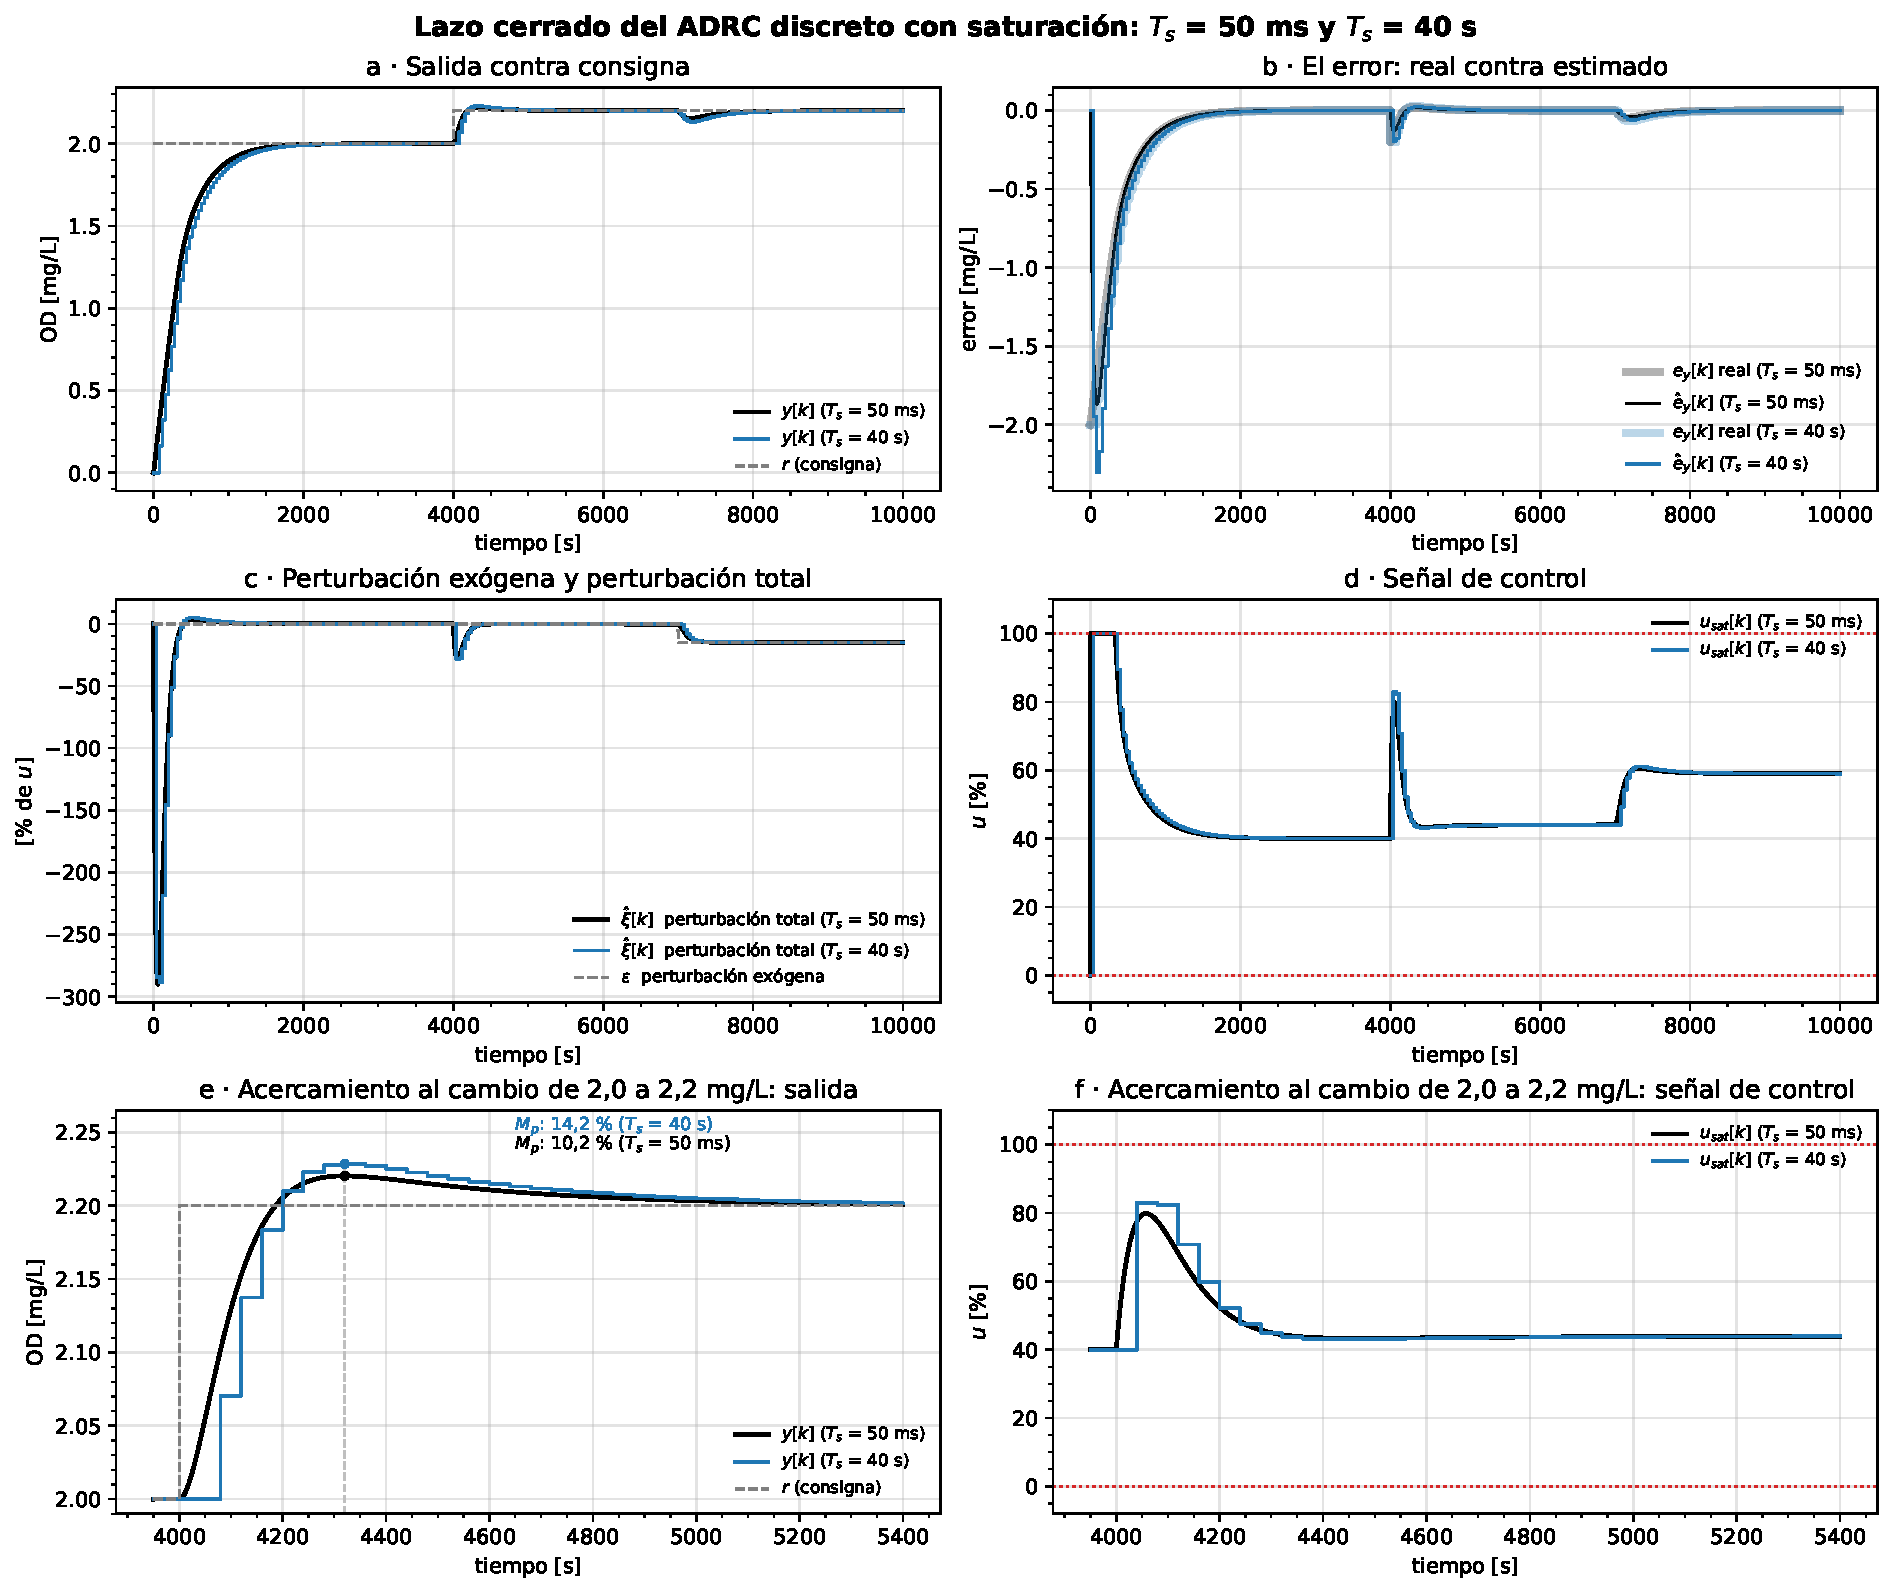
\includegraphics[width=\textwidth]{adrc_discreto_lazo_cerrado.pdf}
  \caption[Lazo cerrado del ADRC discreto con $T_s = 50$~ms y $T_s = 40$~s]{Lazo
    cerrado del ADRC diseñado en discreto, con la planta, el soplador
    limitado entre $0$ y $100~\%$ y el mismo escenario de la
    Figura~\ref{fig:adrc_lazo_cerrado_saturacion}, con $T_s = 50$~ms y
    $T_s = 40$~s, dibujadas en escalones. (a) Salida muestreada $y[k]$ contra
    la consigna. (b) Error de seguimiento real y estimado. (c) Perturbación
    exógena y perturbación total, en \% de $u$. (d) Señal de control.
    (e) y (f) Acercamiento al cambio de consigna de $2{,}0$ a $2{,}2$~mg/L; en (e),
    el sobrepico $M_p$ de cada caso.}
  \label{fig:adrc_discreto_lazo_cerrado}
\end{figure}

\paragraph{Ecuaciones en diferencias.} Para facilitar la implementación en equipos digitales, el
observador se expresa en ecuaciones en diferencias; como el sistema es de orden dos, se tienen dos
ecuaciones en diferencias, una para cada estado estimado. Con
$\widehat{\mathbf{X}}[k] = [\hat{x}_1[k]\ \ \hat{x}_2[k]]^{\top}$, donde
$\hat{x}_1$ estima $e_y$ y $\hat{x}_2$ estima $\xi$, el observador
\eqref{eq:disc_observador} con la orden aplicada es
\begin{equation}
\begin{gathered}
\widehat{\mathbf{X}}[k+1] = \bigl(\mathbf{A}_d - \mathbf{L}_d\,\mathbf{C}_d\bigr)\,\widehat{\mathbf{X}}[k]
+ \mathbf{B}_d\,b_0\,u_{\mathrm{sat}}[k] + \mathbf{L}_d\,e_y[k],
\\[6pt]
\mathbf{A}_d - \mathbf{L}_d\,\mathbf{C}_d =
\begin{bmatrix} a_{11} - l_{1,d}\,c_1 & a_{12} - l_{1,d}\,c_2 \\ a_{21} - l_{2,d}\,c_1 & a_{22} - l_{2,d}\,c_2 \end{bmatrix} .
\end{gathered}
\end{equation}
Fila por fila:
\begin{equation}
\begin{aligned}
\hat{x}_1[k+1] &= (a_{11} - l_{1,d}\,c_1)\,\hat{x}_1[k] + (a_{12} - l_{1,d}\,c_2)\,\hat{x}_2[k] + b_{1,d}\,b_0\,u_{\mathrm{sat}}[k] + l_{1,d}\,e_y[k], \\[2pt]
\hat{x}_2[k+1] &= (a_{21} - l_{2,d}\,c_1)\,\hat{x}_1[k] + (a_{22} - l_{2,d}\,c_2)\,\hat{x}_2[k] + b_{2,d}\,b_0\,u_{\mathrm{sat}}[k] + l_{2,d}\,e_y[k] .
\end{aligned}
\end{equation}
Con $a_{11} = 1$, $a_{12} = T_s$, $a_{21} = 0$, $a_{22} = 1$, $b_{1,d} = T_s$,
$b_{2,d} = 0$, $c_1 = 1$ y $c_2 = 0$ (Tabla~\ref{tab:disc_matrices}):
\begin{equation}
\begin{aligned}
\hat{x}_1[k+1] &= (1 - l_{1,d})\,\hat{x}_1[k] + T_s\,\hat{x}_2[k] + T_s\,b_0\,u_{\mathrm{sat}}[k] + l_{1,d}\,e_y[k], \\[2pt]
\hat{x}_2[k+1] &= -\,l_{2,d}\,\hat{x}_1[k] + \hat{x}_2[k] + l_{2,d}\,e_y[k] .
\end{aligned}
\label{eq:disc_filas}
\end{equation}
Para implementarlo se escribe con retardos, desplazando un periodo
($k \to k-1$):
\begin{equation}
\begin{aligned}
\hat{x}_1[k] &= (1 - l_{1,d})\,\hat{x}_1[k-1] + T_s\,\hat{x}_2[k-1] + T_s\,b_0\,u_{\mathrm{sat}}[k-1] + l_{1,d}\,e_y[k-1], \\[2pt]
\hat{x}_2[k] &= -\,l_{2,d}\,\hat{x}_1[k-1] + \hat{x}_2[k-1] + l_{2,d}\,e_y[k-1] .
\end{aligned}
\label{eq:disc_filas_retardos}
\end{equation}
Las dos ecuaciones usan solo valores del periodo anterior; en el PLC se
calculan con copias de $\hat{x}_1[k-1]$ y $\hat{x}_2[k-1]$, es decir, con la información de cada
variable guardada previamente en memoria, para que
$\hat{x}_2[k]$ no use el $\hat{x}_1[k]$ ya actualizado.
La ley de control \eqref{eq:disc_ley}, con $\mathbf{K}_d = [k_{p,d}\ \ \mathbf{C}_{\xi,d}] = [k_{p,d}\ \ 1]$, es
\begin{equation}
u_0[k] = -\bigl(k_{p,d}\,\hat{x}_1[k] + \hat{x}_2[k]\bigr),
\qquad
u[k] = \frac{u_0[k]}{b_0},
\qquad
u_{\mathrm{sat}}[k] = \operatorname{sat}_{0}^{100}\bigl(u[k]\bigr) .
\label{eq:disc_ley_escalar}
\end{equation}
$u_0$ es la orden normalizada que actúa sobre la cadena de integradores; $b_0$
solo convierte entre $u_0$ y la orden del soplador, a la salida
($u = u_0/b_0$) y en la realimentación al observador ($b_0\,u_{\mathrm{sat}}$).
Con $T_s = 50$~ms, $k_{p,d}$, $l_{1,d}/T_s$ y $l_{2,d}/T_s$ difieren de
$\omega_c$, $2\omega_o$ y $\omega_o^2$ en menos de $0{,}1~\%$
(Tabla~\ref{tab:disc_matrices}).
\paragraph{Realización con retardos.} Las ecuaciones \eqref{eq:disc_filas_retardos}
y \eqref{eq:disc_ley_escalar} se realizan con dos retardos, uno por estado del
observador (Figura~\ref{fig:adrc_discreto_retardos}); en resumen, son necesarios dos retardos y
tres bloques de suma para implementarlo en cualquier equipo digital.

\begin{figure}[H]
  \centering
  \resizebox{\textwidth}{!}{%
  \begin{tikzpicture}[every path/.style={thick}, >={Stealth},
        g/.style={draw, thick, minimum width=1.25cm, minimum height=0.65cm, inner sep=2pt},
        dl/.style={draw, thick, minimum width=1.0cm, minimum height=0.7cm},
        blk/.style={draw, thick, minimum size=0.8cm}]
    % ganancias del observador
    \node[g] (g1a) at (3.9, 1.5) {$l_{1,d}$};
    \node[g] (g1b) at (3.9, 0.5) {$T_s\,b_0$};
    \node[g] (g1c) at (3.9,-0.5) {$1 - l_{1,d}$};
    \node[g] (g1d) at (3.9,-1.5) {$T_s$};
    \node[g] (g2a) at (3.9,-3.5) {$l_{2,d}$};
    \node[g] (g2b) at (3.9,-4.5) {$-l_{2,d}$};
    \node[g] (g2c) at (3.9,-5.5) {$1$};
    \node[sum, minimum size=0.5cm] (S1) at (5.9, 0)   {$+$};
    \node[sum, minimum size=0.5cm] (S2) at (5.9,-4.5) {$+$};
    \node[dl] (D1) at (8.3, 0)   {$z^{-1}$};
    \node[dl] (D2) at (8.3,-4.5) {$z^{-1}$};
    \foreach \n in {g1a,g1b,g1c,g1d} \draw[->] (\n.east) -- (S1);
    \foreach \n in {g2a,g2b,g2c} \draw[->] (\n.east) -- (S2);
    \draw[->] (S1.east) -- node[above] {$\hat{x}_1[k+1]$} (D1.west);
    \draw[->] (S2.east) -- node[above] {$\hat{x}_2[k+1]$} (D2.west);
    \draw (D1.east) -- (9.9,0);
    \draw (D2.east) -- (9.9,-4.5);
    \fill (9.9,0) circle (1.5pt);
    \fill (9.9,-4.5) circle (1.5pt);
    \node[above right] at (8.85,0) {$\hat{x}_1[k]$};
    \node[above right] at (8.85,-4.5) {$\hat{x}_2[k]$};

    % entrada e_y[k]
    \draw (-0.8,1.5) node[left] {$e_y[k]$} -- (0.8,1.5);
    \fill (0.8,1.5) circle (1.5pt);
    \draw[->] (0.8,1.5) -- (g1a.west);
    \draw (0.8,1.5) -- (0.8,-3.5);
    \draw[->] (0.8,-3.5) -- (g2a.west);

    % realimentacion de x1 (por arriba) y de x2 (por abajo)
    \draw (9.9,0) -- (9.9,2.6) -- (2.0,2.6) -- (2.0,-4.5);
    \fill (2.0,-0.5) circle (1.5pt);
    \draw[->] (2.0,-0.5) -- (g1c.west);
    \draw[->] (2.0,-4.5) -- (g2b.west);
    \draw (9.9,-4.5) -- (9.9,-6.6) -- (2.6,-6.6) -- (2.6,-1.5);
    \fill (2.6,-5.5) circle (1.5pt);
    \draw[->] (2.6,-5.5) -- (g2c.west);
    \draw[->] (2.6,-1.5) -- (g1d.west);

    % ley de control
    \node[g] (kp) at (11.5, 0)   {$-k_{p,d}$};
    \node[g] (k1) at (11.5,-4.5) {$-1$};
    \node[sum, minimum size=0.5cm] (S3) at (13.2,-2.25) {$+$};
    \node[blk] (ib) at (14.7,-2.25) {$1/b_0$};
    \draw[->] (9.9,0) -- (kp.west);
    \draw[->] (9.9,-4.5) -- (k1.west);
    \draw[->] (kp.east) -- (S3);
    \draw[->] (k1.east) -- (S3);
    \draw[->] (S3.east) -- node[above] {$u_0[k]$} (ib.west);
    \draw[->] (ib.east) -- (16.8,-2.25) node[right] {$u[k]$};

    % orden aplicada al observador
    \draw[->] (-0.8,0.5) node[left] {$u_{\mathrm{sat}}[k]$} -- (g1b.west);
  \end{tikzpicture}%
  }
  \caption[Realización con retardos del ADRC discreto]{Realización con
    retardos del ADRC discreto: observador \eqref{eq:disc_filas_retardos} y ley
    de control \eqref{eq:disc_ley_escalar}. A la entrada de cada $z^{-1}$ está
    $\hat{x}_i[k+1]$ y a la salida $\hat{x}_i[k]$; la orden aplicada
    $u_{\mathrm{sat}}[k]$ entra al observador con la ganancia $T_s\,b_0$.}
  \label{fig:adrc_discreto_retardos}
\end{figure}

%--------------------------------------------------------------------
\subsection{GPI discreto}
\label{subsec:disc_gpi}

Cada función de transferencia del lazo de las
Figuras~\ref{fig:gpi_antiwindup_ganancias} y~\ref{fig:gpi_antiwindup_wo} se discretiza con
Tustin \eqref{eq:disc_metodos}, el método que más se parece al continuo en la
Figura~\ref{fig:disc_metodos_bode_40}: $H_1 = P/E_1$ (entra $-e_y$, sale $v_1$),
$H_2 = (L - E_1)/E_1$ (entra $u_{\mathrm{sat}}$, sale $v_2$) y la planta $G$ (entra
$\bar{u}$, sale $y$); $1/b_0$ es una ganancia estática y no cambia. Con los dos $E_1$,
\eqref{eq:aw_gpi} y \eqref{eq:aw_gpi_wo}, $H_1$ y $H_2$ son de grado $2$ sobre grado $2$ con el
mismo denominador, así que con $s \to \frac{2}{T_s}\,\frac{1 - z^{-1}}{1 + z^{-1}}$ quedan con
la misma forma:
\begin{equation}
\begin{aligned}
H_1(s) &= \frac{P(s)}{E_1(s)} & \;\longrightarrow\; H_1(z) &= \frac{\beta_0 + \beta_1 z^{-1} + \beta_2 z^{-2}}{1 + \alpha_1 z^{-1} + \alpha_2 z^{-2}}, \\[6pt]
H_2(s) &= \frac{L(s) - E_1(s)}{E_1(s)} & \;\longrightarrow\; H_2(z) &= \frac{\bar{\gamma}_0 + \bar{\gamma}_1 z^{-1} + \bar{\gamma}_2 z^{-2}}{1 + \alpha_1 z^{-1} + \alpha_2 z^{-2}}, \\[6pt]
G(s) &= \frac{k_{dc}}{\tau s + 1} & \;\longrightarrow\; G(z) &= \frac{\beta_g\,\bigl(1 + z^{-1}\bigr)}{1 + \alpha_g z^{-1}} .
\end{aligned}
\label{eq:disc_gpi_tf}
\end{equation}
Solo cambian los valores de los coeficientes, dependiendo de si se usa $E_1 = s^2 + k_2 s + k_1$
o $E_1 = (s + \omega_o)^2$ (Tabla~\ref{tab:disc_gpi_coef}).


\begin{table}[H]
\centering
\caption[Coeficientes del GPI y de la planta discretizados con Tustin]{Coeficientes
  de \eqref{eq:disc_gpi_tf} con los dos $E_1$, con $k_0$, $k_1$ y $k_2$ de la
  Sección~\ref{sec:gpi_caso} y $b_0 = 4{,}1667\times10^{-5}$.}
\label{tab:disc_gpi_coef}
\renewcommand{\arraystretch}{1.3}
\small
\begin{tabular}{llll}
\toprule
 & \textbf{Expresión} & $\boldsymbol{T_s = 50}$~\textbf{ms} & $\boldsymbol{T_s = 40}$~\textbf{s} \\
\midrule
\multicolumn{4}{l}{\textbf{Con las ganancias}, $E_1 = s^2 + k_2 s + k_1$ \eqref{eq:aw_gpi}} \\
$D_0$      & $4 + 2k_2 T_s + k_1 T_s^2$                    & $4{,}0036676$              & $7{,}5555556$ \\
$\alpha_1$ & $(2k_1 T_s^2 - 8)/D_0$                        & $-1{,}99816737$            & $-0{,}89411765$ \\
$\alpha_2$ & $(4 - 2k_2 T_s + k_1 T_s^2)/D_0$              & $0{,}99816835$             & $0{,}22352941$ \\
$\beta_0$  & $(k_0 T_s^2 + 2k_1 T_s)/D_0$                  & $9{,}71389\times10^{-6}$   & $4{,}31373\times10^{-3}$ \\
$\beta_1$  & $2k_0 T_s^2/D_0$                              & $1{,}15635\times10^{-9}$   & $3{,}92157\times10^{-4}$ \\
$\beta_2$  & $(k_0 T_s^2 - 2k_1 T_s)/D_0$                  & $-9{,}71274\times10^{-6}$  & $-3{,}92157\times10^{-3}$ \\
$\bar{\gamma}_0$ & $-k_1 T_s^2/D_0 = -\rho$                      & $-2{,}42833\times10^{-7}$  & $-8{,}23529\times10^{-2}$ \\
$\bar{\gamma}_1$ & $-2k_1 T_s^2/D_0 = -2\rho$                    & $-4{,}85666\times10^{-7}$  & $-1{,}64706\times10^{-1}$ \\
$\bar{\gamma}_2$ & $-k_1 T_s^2/D_0 = -\rho$                      & $-2{,}42833\times10^{-7}$  & $-8{,}23529\times10^{-2}$ \\
\midrule
\multicolumn{4}{l}{\textbf{Con el observador}, $E_1 = (s + \omega_o)^2$ \eqref{eq:aw_gpi_wo}} \\
$D_0$      & $(2 + \omega_o T_s)^2$                                         & $4{,}0033340$              & $7{,}1111111$ \\
$\alpha_1$ & $-2\,(4 - \omega_o^2 T_s^2)/D_0$                               & $-1{,}99833403$            & $-1$ \\
$\alpha_2$ & $(2 - \omega_o T_s)^2/D_0$                                     & $0{,}99833472$             & $0{,}25$ \\
$\beta_0$  & $\omega_o T_s\,[\omega_c\omega_o T_s + 2(\omega_o + 2\omega_c)]/D_0$ & $9{,}71470\times10^{-6}$ & $4{,}58333\times10^{-3}$ \\
$\beta_1$  & $2\,\omega_c\omega_o^2 T_s^2/D_0$                              & $1{,}15644\times10^{-9}$   & $4{,}16667\times10^{-4}$ \\
$\beta_2$  & $\omega_o T_s\,[\omega_c\omega_o T_s - 2(\omega_o + 2\omega_c)]/D_0$ & $-9{,}71355\times10^{-6}$ & $-4{,}16667\times10^{-3}$ \\
$\bar{\gamma}_0$ & $T_s\,(2\omega_c - \omega_o^2 T_s)/D_0$                        & $8{,}30905\times10^{-5}$   & $-0{,}025$ \\
$\bar{\gamma}_1$ & $-2\,\omega_o^2 T_s^2/D_0$                                     & $-3{,}46933\times10^{-7}$  & $-0{,}125$ \\
$\bar{\gamma}_2$ & $-T_s\,(2\omega_c + \omega_o^2 T_s)/D_0$                       & $-8{,}34374\times10^{-5}$  & $-0{,}1$ \\
\midrule
\multicolumn{4}{l}{\textbf{Planta}} \\
$\beta_g$  & $k_{dc}\,T_s/(2\tau + T_s)$                   & $1{,}04164\times10^{-6}$   & $8{,}19672\times10^{-4}$ \\
$\alpha_g$ & $(T_s - 2\tau)/(2\tau + T_s)$                 & $-0{,}99995833$            & $-0{,}96721311$ \\
\bottomrule
\end{tabular}
\end{table}


Ahora bien, la Figura~\ref{fig:gpi_discreto} muestra cómo queda el lazo cerrado en discreto con los
bloques $H_1$ y $H_2$ y sus respectivos coeficientes. Hay que recordar que, cuando el sistema no se
satura, $u = v$ y la dinámica vuelve a ser la diseñada.


\begin{figure}[H]
  \centering
  \resizebox{\textwidth}{!}{%
  \begin{tikzpicture}[every path/.style={thick}]
    \node[sum] (s1) at (1.0,0) {};
    \node[block, minimum width=4.2cm, minimum height=1.3cm] (pe) at (5.0,0)
      {$\dfrac{\beta_0 + \beta_1 z^{-1} + \beta_2 z^{-2}}{1 + \alpha_1 z^{-1} + \alpha_2 z^{-2}}$};
    \node[above=1pt of pe] {$H_1(z)$};
    \node[block, minimum size=9mm] (ib) at (8.8,0) {$1/b_0$};
    \node[sum] (s2) at (10.2,0) {};

    % saturacion (icono clasico de Simulink)
    \node[block, minimum size=11mm] (sat) at (12.2,0) {};
    \draw[thin, gray] ($(sat.center)+(-0.38,0)$) -- ($(sat.center)+(0.38,0)$);
    \draw[thin, gray] ($(sat.center)+(0,-0.38)$) -- ($(sat.center)+(0,0.38)$);
    \draw[line width=1.1pt] ($(sat.center)+(-0.38,-0.22)$) -- ($(sat.center)+(-0.18,-0.22)$)
                         -- ($(sat.center)+(0.18,0.22)$) -- ($(sat.center)+(0.38,0.22)$);
    \node[above=1pt of sat, font=\small] {0--100~\%};

    \coordinate (us) at (14.8,0);
    \node[block, minimum width=4.2cm, minimum height=1.3cm] (fb) at (12.5,-2.1)
      {$\dfrac{\bar{\gamma}_0 + \bar{\gamma}_1 z^{-1} + \bar{\gamma}_2 z^{-2}}{1 + \alpha_1 z^{-1} + \alpha_2 z^{-2}}$};
    \node[below=1pt of fb] {$H_2(z)$};
    \node[sum] (s3) at (16.3,0) {};
    \node[block, minimum width=1.6cm, minimum height=1.1cm] (plant) at (18.6,0) {$G(z)$};
    \coordinate (yb) at (20.1,0);

    % --- recuadro del controlador ---
    \draw[red, dashed, thick] (2.5,1.75) rectangle (15.2,-3.35);
    \node[below left] at (15.2,1.75) {GPI discreto};

    % --- señales ---
    \draw[->] (-0.9,0) node[above right] {$r[k]$} -- (s1.west);
    \node[sgn] at ($(s1.west)+(-0.15,0.25)$) {$+$};
    \draw[->] (s1.east) -- node[above, pos=0.4] {$-e_y[k]$} (pe.west);
    \draw[->] (pe.east) -- node[above] {$v_1[k]$} (ib.west);
    \draw[->] (ib.east) -- (s2.west);
    \node[sgn] at ($(s2.west)+(-0.2,0.25)$) {$+$};
    \draw[->] (s2.east) -- node[above] {$v[k]$} (sat.west);
    \draw (sat.east) -- node[above] {$u_{\mathrm{sat}}[k]$} (us);
    \fill (us) circle (1.5pt);
    \draw[->] (us) -- (s3.west);
    \node[sgn] at ($(s3.west)+(-0.2,-0.25)$) {$+$};
    \draw[->] (s3 |- 0,1.6) node[above] {$\varepsilon[k]$} -- (s3.north);
    \node[sgn] at ($(s3.north)+(-0.25,0.2)$) {$+$};
    \draw[->] (s3.east) -- node[above] {$\bar{u}[k]$} (plant.west);
    \draw[->] (us) -- (us |- fb) -- (fb.east);
    \draw[->] (fb.west) -- (s2 |- fb) -- node[left, pos=0.5] {$v_2[k]$} (s2.south);
    \node[sgn] at ($(s2.south)+(0.25,-0.2)$) {$-$};
    \draw (plant.east) -- (yb);
    \draw[->] (yb) -- (21.2,0) node[above left] {$y[k]$};
    \fill (yb) circle (1.5pt);
    \draw[->] (yb) -- (20.1,-3.9) -- (1.0,-3.9) -- (s1.south);
    \node[sgn] at ($(s1.south)+(-0.25,-0.15)$) {$-$};
  \end{tikzpicture}%
  }
  \caption[GPI discreto con realimentación de la saturación]{GPI discreto con
    realimentación de la saturación: cada bloque de las
    Figuras~\ref{fig:gpi_antiwindup_ganancias} y~\ref{fig:gpi_antiwindup_wo} y la planta
    discretizados con Tustin \eqref{eq:disc_gpi_tf}. La estructura es la misma con los dos
    $E_1$; solo cambian los coeficientes (Tabla~\ref{tab:disc_gpi_coef}).}
  \label{fig:gpi_discreto}
\end{figure}
\paragraph{Simulación.} En el cambio de consigna de $2{,}0$ a $2{,}2$~mg/L el
soplador no se satura, así que $u = v$ y, con cualquiera de los dos $E_1$, el controlador es
$C(z) = \frac{1}{b_0}\,H_1(z)/\bigl(1 + H_2(z)\bigr)$, exactamente el Tustin de
$C(s)$. La Figura~\ref{fig:gpi_discreto_vs_adrc} compara ese lazo, con la
planta también por Tustin, con el ADRC discreto de la
Figura~\ref{fig:adrc_discreto_lazo_cerrado}. Con $T_s = 50$~ms coinciden; con
$T_s = 40$~s el GPI responde desde la misma muestra del cambio, porque Tustin, en su realización,
deja términos directos en el controlador ($\beta_0$) y en la planta ($\beta_g$), mientras que el
ADRC usa el error del periodo anterior. Esto quiere decir que Tustin tiende a estar más en fase y no
se atrasa tanto como otras discretizaciones.

\begin{figure}[H]
  \centering
  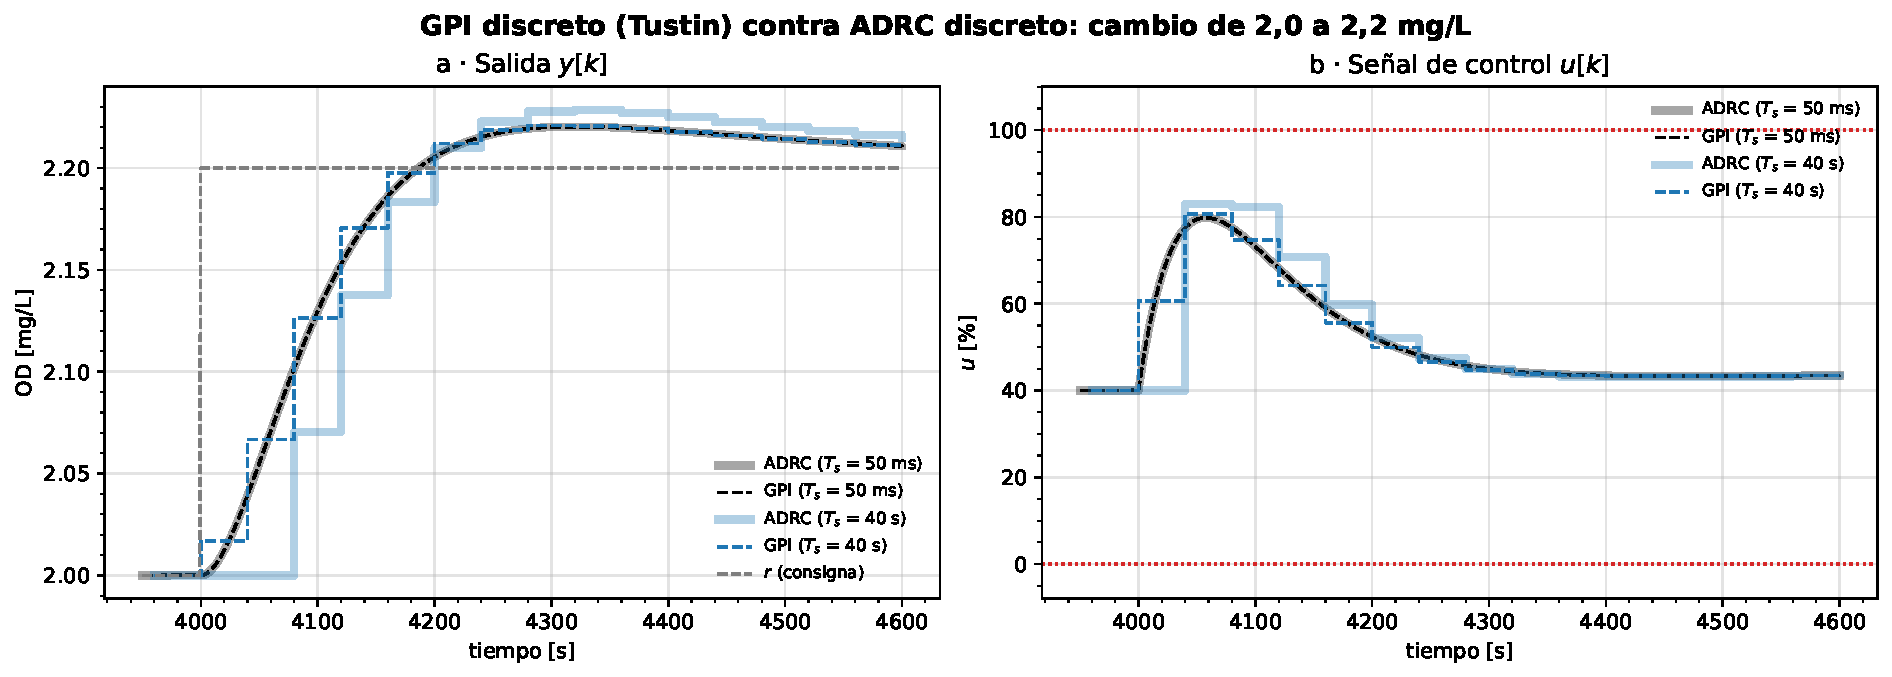
\includegraphics[width=\textwidth]{gpi_discreto_vs_adrc.pdf}
  \caption[GPI discreto contra ADRC discreto]{GPI discreto con
    $E_1 = (s + \omega_o)^2$ \eqref{eq:aw_gpi_wo}, con controlador y
    planta por Tustin (discontinua), contra ADRC discreto con la planta exacta
    (banda), en el cambio de consigna de $2{,}0$ a $2{,}2$~mg/L, sin
    saturación, con $T_s = 50$~ms (negro) y $T_s = 40$~s (azul), dibujados en
    escalones. (a) Salida $y[k]$. (b) Señal de control $u[k]$.}
  \label{fig:gpi_discreto_vs_adrc}
\end{figure}

\paragraph{Ecuaciones en diferencias.} Para facilitar la implementación, las funciones de
transferencia en $z$ se pasan a ecuaciones en diferencias en el tiempo discreto, con $x[k] = -e_y[k]$:
\begin{equation}
\begin{aligned}
v_1[k] &= \beta_0\,x[k] + \beta_1\,x[k-1] + \beta_2\,x[k-2] - \alpha_1\,v_1[k-1] - \alpha_2\,v_1[k-2], \\[2pt]
v_2[k] &= \bar{\gamma}_0\,u_{\mathrm{sat}}[k] + \bar{\gamma}_1\,u_{\mathrm{sat}}[k-1] + \bar{\gamma}_2\,u_{\mathrm{sat}}[k-2] - \alpha_1\,v_2[k-1] - \alpha_2\,v_2[k-2], \\[2pt]
v[k] &= \frac{v_1[k]}{b_0} - v_2[k], \qquad u_{\mathrm{sat}}[k] = \operatorname{sat}_{0}^{100}\bigl(v[k]\bigr) .
\end{aligned}
\label{eq:disc_gpi_dif}
\end{equation}
\paragraph{Realización.} Como $H_1$ y $H_2$ comparten el denominador, los dos
bloques se realizan juntos en forma directa I \cite{chen1993analog}, con
entradas $-e_y[k]$ y $u_{\mathrm{sat}}[k]$ y salida $v[k]$
(Figura~\ref{fig:disc_formas_directas}). De
$v = H_1\,(-e_y)/b_0 - H_2\,u_{\mathrm{sat}}$, la función de transferencia
discreta completa del controlador tiene dos entradas y una salida, y se puede escribir en la
siguiente forma compacta:
\begin{equation}
V(z) =
\begin{bmatrix}
\dfrac{\beta_0 + \beta_1 z^{-1} + \beta_2 z^{-2}}{b_0\,\bigl(1 + \alpha_1 z^{-1} + \alpha_2 z^{-2}\bigr)}
&
\dfrac{-\bigl(\bar{\gamma}_0 + \bar{\gamma}_1 z^{-1} + \bar{\gamma}_2 z^{-2}\bigr)}{1 + \alpha_1 z^{-1} + \alpha_2 z^{-2}}
\end{bmatrix}
\begin{bmatrix} -E_y(z) \\[4pt] U_{\mathrm{sat}}(z) \end{bmatrix},
\label{eq:disc_gpi_miso}
\end{equation}
y en forma directa I, con $x[k] = -e_y[k]$:
\begin{equation}
\begin{aligned}
v[k] = {} & \frac{\beta_0\,x[k] + \beta_1\,x[k-1] + \beta_2\,x[k-2]}{b_0}
- \bigl(\bar{\gamma}_0\,u_{\mathrm{sat}}[k] + \bar{\gamma}_1\,u_{\mathrm{sat}}[k-1] + \bar{\gamma}_2\,u_{\mathrm{sat}}[k-2]\bigr) \\
& - \alpha_1\,v[k-1] - \alpha_2\,v[k-2] .
\end{aligned}
\label{eq:disc_gpi_fd1}
\end{equation}
Son seis retardos y un solo sumador. Los estados son señales del lazo, con
rangos conocidos, y se pueden inicializar al arrancar. Hay que trabajar en doble precisión (LREAL en el PLC, de 64 bits, y no REAL de 32 bits): con $T_s = 50$~ms los polos de
$E_1(z)$ están en $|z| = 0{,}99908$ con las ganancias y en $0{,}99917$ (doble) con el
observador, y $1 + \alpha_1 + \alpha_2$ vale $9{,}7\times10^{-7}$ y $6{,}9\times10^{-7}$; por
eso $\alpha_1$ y $\alpha_2$ llevan ocho decimales.

\begin{figure}[H]
  \centering
  \resizebox{0.75\textwidth}{!}{%
  \begin{tikzpicture}[every path/.style={thick},
      g/.style={draw, thick, minimum width=0.9cm, minimum height=0.7cm, inner sep=2pt},
      dl/.style={draw, thick, minimum width=0.95cm, minimum height=0.6cm}]
    % --- entrada -e_y ---
    \node[g] (a0) at (2.9,0)    {$\beta_0/b_0$};
    \node[g] (a1) at (2.9,-1.6) {$\beta_1/b_0$};
    \node[g] (a2) at (2.9,-3.2) {$\beta_2/b_0$};
    \node[dl] (dx1) at (0.9,-0.8) {$z^{-1}$};
    \node[dl] (dx2) at (0.9,-2.4) {$z^{-1}$};
    % --- entrada u_sat ---
    \node[g] (c0) at (2.9,-4.8) {$-\bar{\gamma}_0$};
    \node[g] (c1) at (2.9,-6.4) {$-\bar{\gamma}_1$};
    \node[g] (c2) at (2.9,-8.0) {$-\bar{\gamma}_2$};
    \node[dl] (du1) at (0.9,-5.6) {$z^{-1}$};
    \node[dl] (du2) at (0.9,-7.2) {$z^{-1}$};
    % --- sumador y salida ---
    \node[sum, minimum size=0.55cm] (S) at (5.2,-4.0) {$+$};
    \node[g] (e1) at (6.4,-5.6) {$-\alpha_1$};
    \node[g] (e2) at (6.4,-7.2) {$-\alpha_2$};
    \node[dl] (dv1) at (7.8,-4.8) {$z^{-1}$};
    \node[dl] (dv2) at (7.8,-6.4) {$z^{-1}$};

    \draw[->] (-0.6,0) node[left] {$-e_y[k]$} -- (a0.west);
    \fill (0.9,0) circle (1.5pt);
    \draw[->] (0.9,0) -- (dx1.north);
    \draw (dx1.south) -- (0.9,-1.6);
    \fill (0.9,-1.6) circle (1.5pt);
    \draw[->] (0.9,-1.6) -- (a1.west);
    \draw[->] (0.9,-1.6) -- (dx2.north);
    \draw (dx2.south) -- (0.9,-3.2);
    \draw[->] (0.9,-3.2) -- (a2.west);
    \node[font=\scriptsize, left] at (0.9,-1.6) {$-e_y[k-1]$};
    \node[font=\scriptsize, left] at (0.9,-3.2) {$-e_y[k-2]$};

    \draw[->] (-0.6,-4.8) node[left] {$u_{\mathrm{sat}}[k]$} -- (c0.west);
    \fill (0.9,-4.8) circle (1.5pt);
    \draw[->] (0.9,-4.8) -- (du1.north);
    \draw (du1.south) -- (0.9,-6.4);
    \fill (0.9,-6.4) circle (1.5pt);
    \draw[->] (0.9,-6.4) -- (c1.west);
    \draw[->] (0.9,-6.4) -- (du2.north);
    \draw (du2.south) -- (0.9,-8.0);
    \draw[->] (0.9,-8.0) -- (c2.west);
    \node[font=\scriptsize, left] at (0.9,-6.4) {$u_{\mathrm{sat}}[k-1]$};
    \node[font=\scriptsize, left] at (0.9,-8.0) {$u_{\mathrm{sat}}[k-2]$};

    \foreach \n in {a0,a1,a2,c0,c1,c2} \draw[->] (\n.east) -- (S);
    \draw[->] (e1.north west) -- (S);
    \draw[->] (e2.north west) -- (S);

    \draw[->] (S.east) -- (9.0,-4.0) node[right] {$v[k]$};
    \fill (7.8,-4.0) circle (1.5pt);
    \draw[->] (7.8,-4.0) -- (dv1.north);
    \draw (dv1.south) -- (7.8,-5.6);
    \fill (7.8,-5.6) circle (1.5pt);
    \draw[->] (7.8,-5.6) -- (e1.east);
    \draw[->] (7.8,-5.6) -- (dv2.north);
    \draw (dv2.south) -- (7.8,-7.2);
    \draw[->] (7.8,-7.2) -- (e2.east);
    \node[font=\scriptsize, right] at (7.8,-5.6) {$v[k-1]$};
    \node[font=\scriptsize, right] at (7.8,-7.2) {$v[k-2]$};
  \end{tikzpicture}%
  }
  \caption[Realización en forma directa I del GPI discreto]{Realización en
    forma directa I de los dos bloques del GPI discreto juntos
    \eqref{eq:disc_gpi_fd1}: entradas $-e_y[k]$ y $u_{\mathrm{sat}}[k]$,
    salida $v[k]$; todas las entradas del sumador suman. Es la misma con los dos $E_1$, con los
    coeficientes de la Tabla~\ref{tab:disc_gpi_coef}.}
  \label{fig:disc_formas_directas}
\end{figure}


%--------------------------------------------------------------------
\subsection{Prefiltro de consigna discreto}
\label{subsec:disc_prefiltro}

El prefiltro \eqref{eq:pref_f} se discretiza con Tustin \eqref{eq:disc_metodos}, igual que el GPI.
Con $s \to \frac{2}{T_s}\,\frac{1 - z^{-1}}{1 + z^{-1}}$,
\begin{equation}
F(s) = \frac{k_0}{k_1 s + k_0}
\quad\longrightarrow\quad
F(z) = \frac{\beta_f\,\bigl(1 + z^{-1}\bigr)}{1 + \alpha_f\,z^{-1}},
\qquad
\alpha_f = \frac{k_0 T_s - 2 k_1}{k_0 T_s + 2 k_1},
\qquad
\beta_f = \frac{k_0 T_s}{k_0 T_s + 2 k_1} .
\label{eq:disc_pref_tf}
\end{equation}
Las dos son ganancias fijas: se calculan una vez y solo cambian con $k_0$, $k_1$ o $T_s$; $k_2$ no
entra. En términos de los anchos de banda,
\begin{equation}
\alpha_f = \frac{\omega_c\,\omega_o\,T_s - 2\,(\omega_o + 2\,\omega_c)}{\omega_c\,\omega_o\,T_s + 2\,(\omega_o + 2\,\omega_c)},
\qquad
\beta_f = \frac{\omega_c\,\omega_o\,T_s}{\omega_c\,\omega_o\,T_s + 2\,(\omega_o + 2\,\omega_c)} .
\end{equation}
La ganancia estática es exactamente $F(1) = 2\beta_f/(1 + \alpha_f) = 1$. Como Tustin es una
sustitución de $s$, el polo de $F(z)$ es la imagen del cero del lazo y la cancelación de
\eqref{eq:pref_yr_f} se conserva exacta con el GPI discreto. La Tabla~\ref{tab:disc_pref} resume los
valores.

\begin{table}[H]
\centering
\caption{Ganancias del prefiltro discreto \eqref{eq:disc_pref_tf}.}
\label{tab:disc_pref}
\renewcommand{\arraystretch}{1.3}
\begin{tabular}{llll}
\toprule
 & \textbf{Expresión} & $\boldsymbol{T_s = 50}$~\textbf{ms} & $\boldsymbol{T_s = 40}$~\textbf{s} \\
\midrule
$\alpha_f$ & $(k_0 T_s - 2 k_1)/(k_0 T_s + 2 k_1)$ & $-0{,}99988096$ & $-0{,}90909091$ \\
$\beta_f$ & $k_0 T_s/(k_0 T_s + 2 k_1)$ & $5{,}952027\times10^{-5}$ & $4{,}545455\times10^{-2}$ \\
\bottomrule
\end{tabular}
\end{table}

\paragraph{Ecuación en diferencias.} Para simplificar la implementación, el prefiltro se presenta
como una ecuación en diferencias:
\begin{equation}
r_f[k] = -\alpha_f\,r_f[k-1] + \beta_f\,\bigl(r[k] + r[k-1]\bigr),
\qquad
e_y[k] = y[k] - r_f[k] .
\label{eq:disc_pref_dif}
\end{equation}
Con $T_s = 50$~ms, $\beta_f$ es del orden de $10^{-5}$, así que hay que trabajar en doble precisión
(LREAL), como en el GPI.

La Figura~\ref{fig:disc_prefiltro_retardo} muestra el cambio de consigna con el prefiltro discreto, con
la planta exacta y con $\theta = 0$ y $50$~s, y la Tabla~\ref{tab:disc_prefiltro_indices} resume sus
índices. En ningún caso hay sobrepico. Con $T_s = 50$~ms, el ADRC y el GPI discretos se comportan
igual: tienen el mismo tiempo de asentamiento y el mismo pico de la señal de control, y el retardo
solo alarga un poco el transitorio y sube el pico de $u$. Cuando se aumenta el tiempo de muestreo a
$T_s = 40$~s ya se ven diferencias: el ADRC se asienta un poco antes, el pico de $u$ sube, sobre todo
con el GPI, y con $\theta = 50$~s aparece una pequeña oscilación en la señal de control. Aun así, en
todos los casos el prefiltro discreto funciona adecuadamente: la salida llega a la consigna sin
sobrepico y la señal de control queda lejos de la saturación. Además, el $t_s$ coincide con el que se
buscó al elegir $\omega_c = 4/\tau$: con $\tau = 20$~min en la planta y el controlador acelerándola a
cuatro veces la velocidad del lazo abierto, el sistema debería estabilizarse cerca de los $20$~min en
lazo cerrado, según el criterio que se use, lo cual es adecuado y se comprueba con este experimento.

\begin{figure}[H]
  \centering
  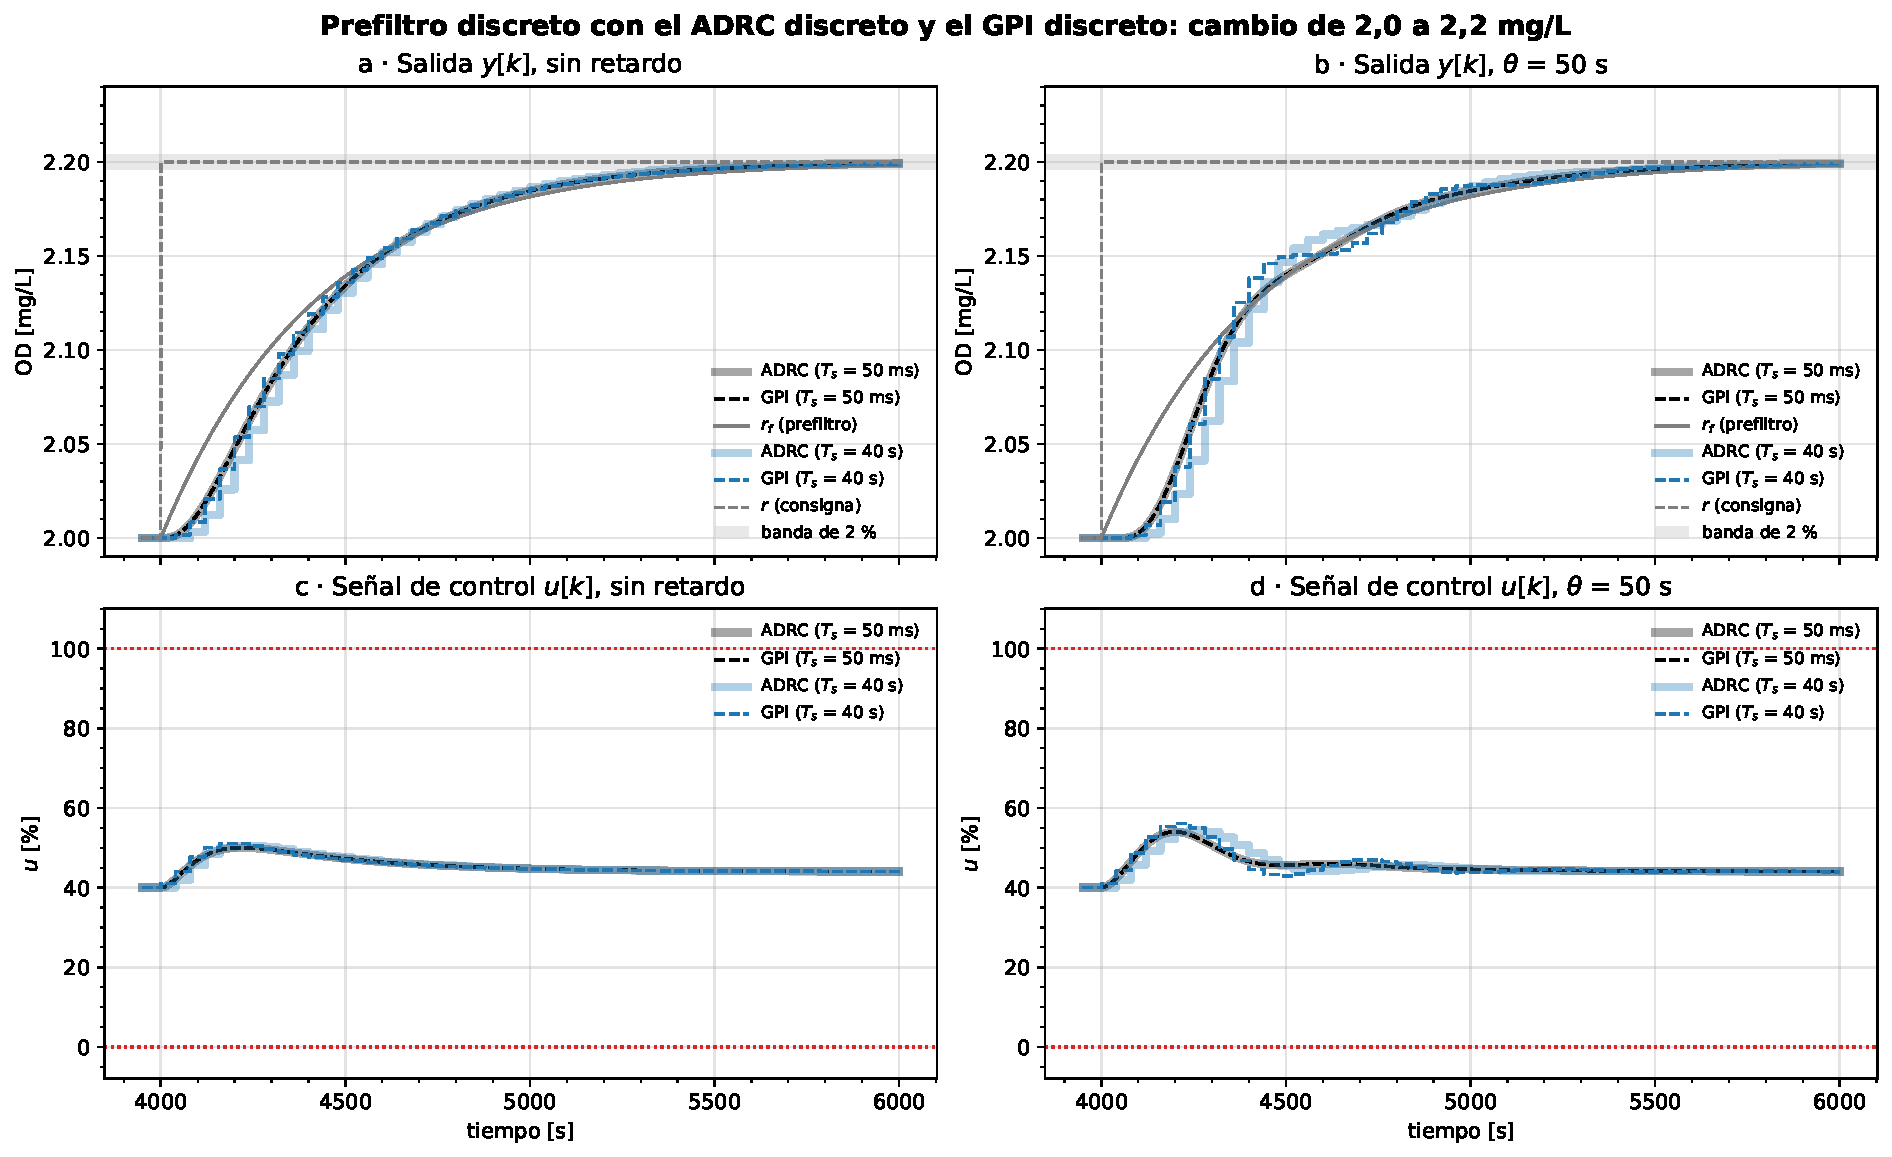
\includegraphics[width=\textwidth]{disc_prefiltro_retardo.pdf}
  \caption[Prefiltro discreto con el ADRC y el GPI discretos]{Cambio de consigna de $2{,}0$ a
    $2{,}2$~mg/L con el prefiltro discreto \eqref{eq:disc_pref_dif}, la planta exacta y el soplador
    limitado entre $0$ y $100~\%$: ADRC discreto (banda) y GPI discreto con
    $E_1 = (s + \omega_o)^2$ (discontinua), con $T_s = 50$~ms (negro) y $T_s = 40$~s (azul),
    dibujados en escalones. (a) y (c) Sin retardo; (b) y (d) con $\theta = 50$~s. Arriba, la
    salida $y[k]$ con la banda de $2~\%$ del escalón; abajo, la señal de control $u[k]$.}
  \label{fig:disc_prefiltro_retardo}
\end{figure}

\begin{table}[H]
\centering
\caption[Índices del cambio de consigna con el prefiltro discreto]{Tiempo de asentamiento $t_s$ y
  pico de la señal de control $u_{\max}$ (Tabla~\ref{tab:metricas}) en el cambio de $2{,}0$ a
  $2{,}2$~mg/L de la Figura~\ref{fig:disc_prefiltro_retardo}. En ningún caso hay sobrepico.}
\label{tab:disc_prefiltro_indices}
\renewcommand{\arraystretch}{1.3}
\begin{tabular}{llcccc}
\toprule
 & & \multicolumn{2}{c}{\textbf{Sin retardo}} & \multicolumn{2}{c}{$\boldsymbol{\theta = 50}$~\textbf{s}} \\
\cmidrule(lr){3-4}\cmidrule(lr){5-6}
\textbf{Controlador} & $\boldsymbol{T_s}$ & $t_s$ [min] & $u_{\max}$ [\%] & $t_s$ [min] & $u_{\max}$ [\%] \\
\midrule
ADRC & $50$~ms & $24{,}4$ & $50{,}0$ & $24{,}7$ & $54{,}0$ \\
GPI  & $50$~ms & $24{,}4$ & $50{,}0$ & $24{,}7$ & $54{,}0$ \\
\midrule
ADRC & $40$~s  & $22{,}7$ & $50{,}5$ & $23{,}7$ & $54{,}5$ \\
GPI  & $40$~s  & $24{,}2$ & $51{,}1$ & $23{,}3$ & $56{,}1$ \\
\bottomrule
\end{tabular}
\end{table}

%--------------------------------------------------------------------
\section{Planta con retardo}
\label{sec:impl_retardo}

La planta de diseño tiene un retardo $\theta = 50$~s
\eqref{eq:ident_planta_diseno} que el observador no conoce: recibe la orden
aplicada en el mismo periodo en que se calcula, mientras que la planta solo la
ve $\theta$ segundos después. Si el retardo se conoce, una solución simple es
sincronizar el observador con la planta retrasando la orden que le entra
\cite[sec.~9.4]{herbst2024adrc}, \cite{herbst2013practical}. Con el observador
discreto \eqref{eq:disc_observador},
\begin{equation}
\widehat{\mathbf{X}}[k+1] = \bigl(\mathbf{A}_d - \mathbf{L}_d\,\mathbf{C}_d\bigr)\,\widehat{\mathbf{X}}[k]
+ \mathbf{B}_d\,b_0\,u_{\mathrm{sat}}[k - n_d] + \mathbf{L}_d\,e_y[k],
\qquad
n_d \approx \frac{\theta}{T_s} ,
\label{eq:disc_retardo}
\end{equation}
y fila por fila solo cambia la primera ecuación de \eqref{eq:disc_filas}:
\begin{equation}
\hat{x}_1[k+1] = (1 - l_{1,d})\,\hat{x}_1[k] + T_s\,\hat{x}_2[k] + T_s\,b_0\,u_{\mathrm{sat}}[k - n_d] + l_{1,d}\,e_y[k] .
\end{equation}
Las matrices, las ganancias $\mathbf{K}_d$ y $\mathbf{L}_d$ y la ley de control
\eqref{eq:disc_ley_escalar} no cambian; lo único que se añade es un registro de
las últimas $n_d$ órdenes aplicadas. Con $T_s = 50$~ms y $\theta = 50$~s,
$n_d = 1000$ muestras.

La Figura~\ref{fig:adrc_discreto_retardo} compara el ADRC discreto sin
sincronizar ($n_d = 0$) y sincronizado ($n_d = \theta/T_s$) para
$\theta = 20$, $40$, $50$, $60$ y $100$~s, con el escalón de consigna de $2{,}0$ a
$2{,}2$~mg/L y la perturbación $\varepsilon = -15~\%$ a los 40~min. Con
$\theta = 50$~s, el pico de oxígeno baja de $2{,}29$ a $2{,}24$~mg/L y la señal
de control deja de oscilar (sin sincronizar baja hasta $29~\%$; sincronizado no
pasa por debajo del $40~\%$ del régimen). En el caso extremo de $100$~s, sin
sincronizar el lazo oscila y el soplador llega a $0$ y a $100~\%$;
sincronizado, el pico es de $2{,}26$~mg/L y la orden no pasa del $86~\%$. A
cambio, la respuesta es algo más lenta ($t_s$ de $17{,}4$ frente a $14{,}7$~min
con $\theta = 50$~s, con banda de $2~\%$ del escalón) y la caída por la
perturbación es un poco mayor ($2{,}129$ frente a $2{,}132$~mg/L), pero sin oscilación, por lo que
sincronizar el observador da mejores respuestas.

El retardo real no se conoce con exactitud: solo se obtuvo visualmente
(Sección~\ref{sec:ident_retardo}), y los diseños se hicieron con $\theta = 50$~s en la planta. Ahora
bien, sobreestimarlo es seguro: con $n_d T_s = 100$~s el pico es de $2{,}23$~mg/L y $t_s$ sube a
$20{,}7$~min. Subestimarlo mejora menos, pero sigue ayudando: con $n_d T_s = 25$~s el pico es de
$2{,}26$~mg/L, frente a $2{,}29$. Por eso es mejor sobreestimar $\theta$ y elegir un valor un poco más
grande.

\begin{figure}[H]
  \centering
  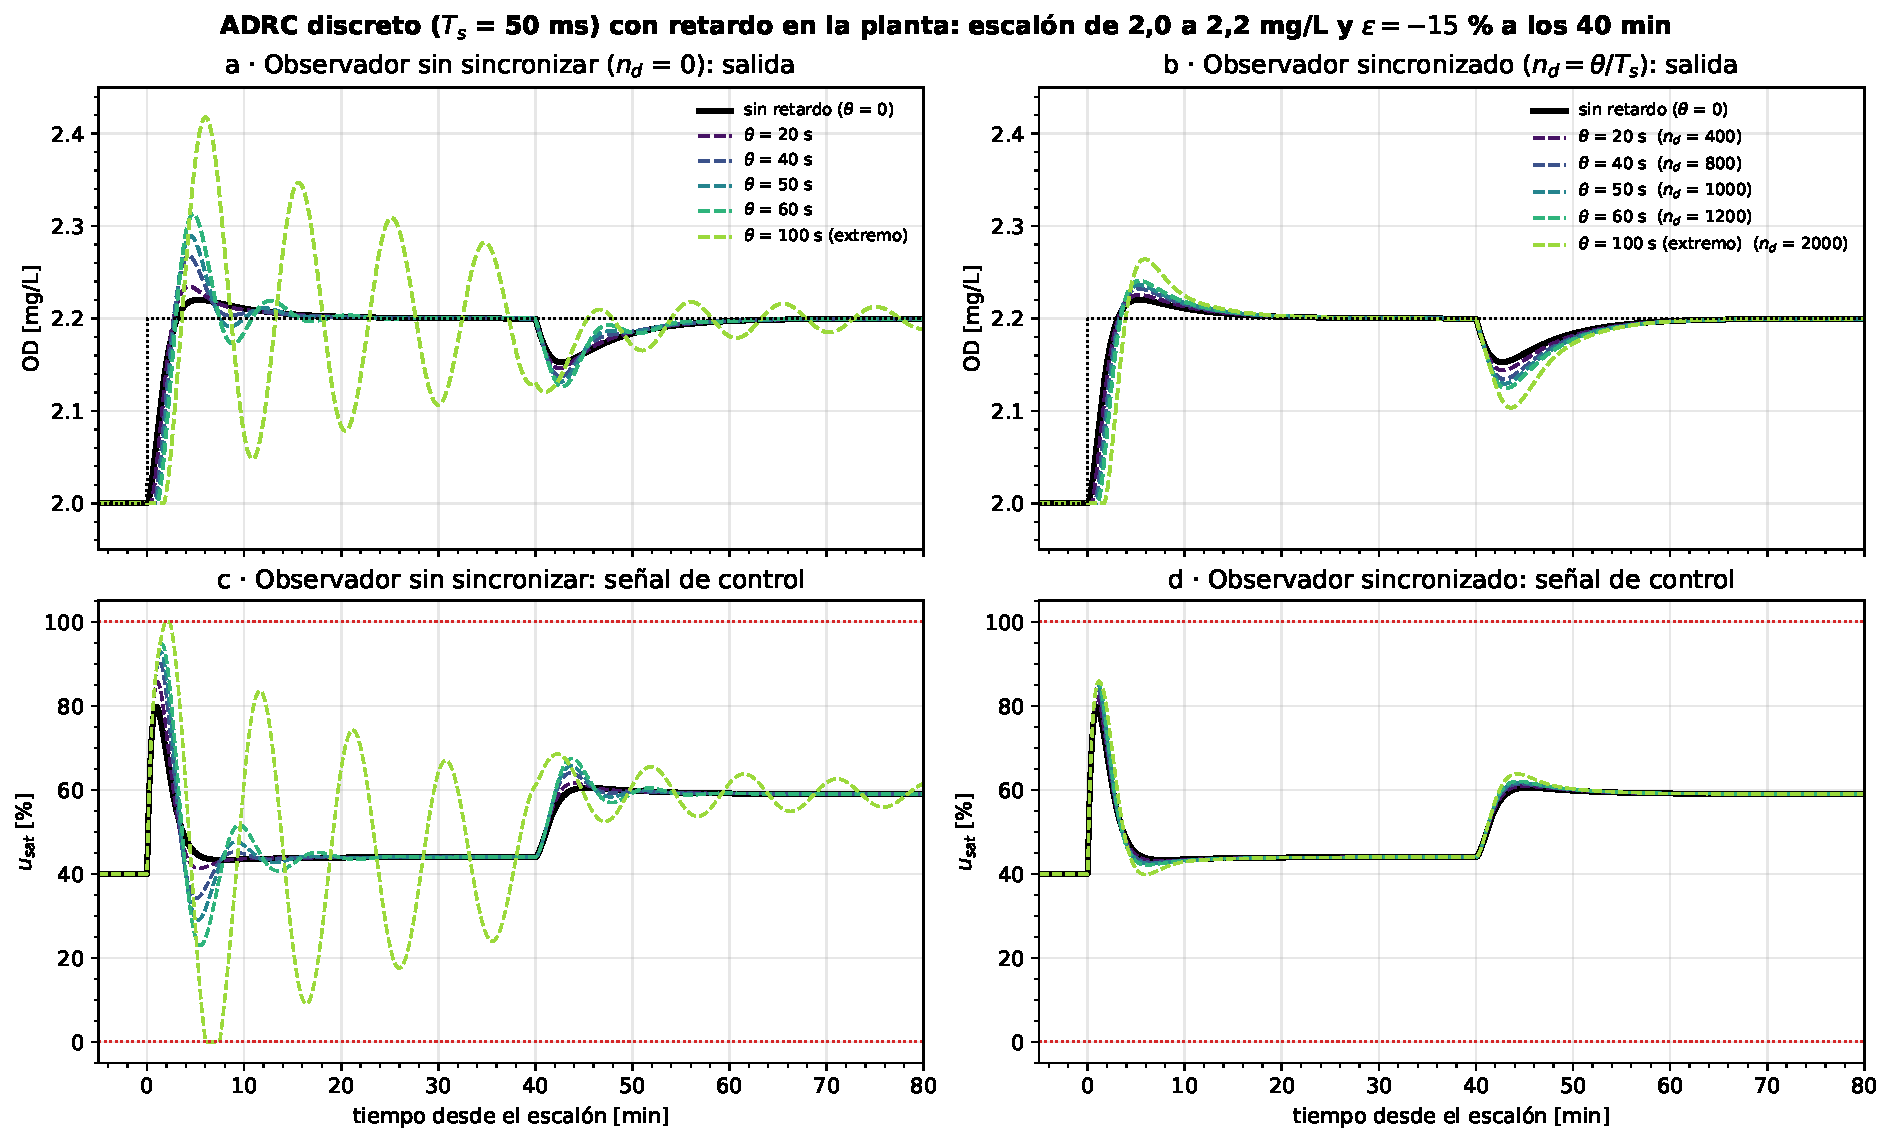
\includegraphics[width=\textwidth]{adrc_discreto_retardo.pdf}
  \caption[ADRC discreto con retardo: observador sin sincronizar y
    sincronizado]{ADRC discreto ($T_s = 50$~ms) con la planta nominal con
    retardo $\theta$ y el soplador limitado entre $0$ y $100~\%$: escalón de
    consigna de $2{,}0$ a $2{,}2$~mg/L y $\varepsilon = -15~\%$ a los 40~min.
    (a) y (c) Observador sin sincronizar ($n_d = 0$); (b) y (d) observador
    sincronizado \eqref{eq:disc_retardo}, con $n_d = \theta/T_s$. Arriba, la
    salida; abajo, la señal de control. En negro, sin retardo.}
  \label{fig:adrc_discreto_retardo}
\end{figure}

%--------------------------------------------------------------------
\section{Implementación en PLC}
\label{sec:impl_plc}
\label{sec:met_plc}
Esta sección contiene el desarrollo de los diseños propuestos anteriormente, llevando los esquemas
de saturación y algunas de las realizaciones que se obtuvieron en discreto a una forma que se pueda
implementar en un PLC. Se parte de una idea de alto nivel, donde se fundamentan las ideas
principales, y cada vez se va formalizando más con los resultados teóricos de las secciones
anteriores, hasta obtener un producto con una metodología bien definida para su implementación.

%--------------------------------------------------------------------
\subsection{Producto digital}
\label{subsec:plc_producto}

Todo producto digital empieza en alto nivel, como una caja negra con sus bloques de entradas y
salidas. Por dentro, cada bloque debe seguir un flujo descrito por una máquina de estados, y eso es
lo que permite integrar productos digitales en procesos industriales. En la industria se manejan
estándares con estados como inicio, arranque y parada de emergencia, entre otros. Aquí, dada la
simplicidad de los bloques, se simplificaron a solo dos estados, \texttt{RESET} y \texttt{AUTOMATIC}
(Figura~\ref{fig:plc_estados}), que ofrecen una configuración para integrarlos en procesos
industriales, ya que con ellos se puede habilitar o deshabilitar el módulo: \texttt{AUTOMATIC} lo
habilita y \texttt{RESET} lo deshabilita.


\begin{figure}[H]
  \centering
  \begin{tikzpicture}[>=Stealth, thick, font=\small,
      est/.style={draw, circle, thick, minimum size=3.2cm, text width=2.9cm, align=center,
        inner sep=0pt, fill=white, font=\footnotesize\bfseries},
      et/.style={font=\footnotesize\ttfamily, fill=white, inner sep=1.5pt, align=center}]
    \node[est] (R) at (0,0) {RESET};
    \node[est] (A) at (7.5,0) {AUTOMATIC};
    \draw[->] (R.25) to[bend left=18] node[et, above=2pt] {RESET = 0 AND Ready} (A.155);
    \draw[->] (A.205) to[bend left=18] node[et, below=2pt] {RESET = 1} (R.335);
  \end{tikzpicture}
  \caption[Máquina de estados de los bloques de función]{Máquina de estados de los bloques de
    función.}
  \label{fig:plc_estados}
\end{figure}

El producto de este trabajo son bloques de función para el PLC. Para el control
son tres: el ADRC basado en observador, el GPI con sus ganancias y el GPI con
los anchos de banda (Tablas~\ref{tab:plc_adrc_eso}, \ref{tab:plc_gpi} y \ref{tab:plc_adrc_gpi}). El
ADRC se sintoniza con $\omega_c$, $\omega_o$ y $b_0$
(Sección~\ref{subsec:sintonia}). El GPI recibe directamente $k_0$, $k_1$, $k_2$
y $b_0$: si se conocen $\omega_c$ y $\omega_o$, las ganancias salen de
\eqref{eq:eso2gpi} y los dos bloques dan el mismo lazo; si no, se sintoniza
como un PI con filtro (Figura~\ref{fig:gpi_pi_filtro}), con $k_1$ y $k_0$ como
acciones proporcional e integral y $k_2$ como polo del filtro. En ese caso nada
garantiza la estabilidad, así que el bloque verifica que $k_0, k_1, k_2 > 0$ y
$k_2 k_1 > k_0$, la condición de Routh--Hurwitz de
$\Delta(s) = s^3 + k_2 s^2 + k_1 s + k_0$ con la planta de diseño, y si no se
cumple conserva las ganancias anteriores. \texttt{ADRC\_GPI} recibe $\omega_c$, $\omega_o$
y $b_0$, calcula $k_0$, $k_1$ y $k_2$ con \eqref{eq:eso2gpi} y usa
$E_1(s) = (s + \omega_o)^2$ \eqref{eq:aw_gpi_wo}, con lo que se comporta igual que el
ADRC también cuando satura. La
consigna y la medida
entran como \texttt{SET\_POINT} y \texttt{ACTUAL}, y dentro se calcula la resta que da el error de
seguimiento; la salida \texttt{U} es la orden al soplador, ya limitada entre \texttt{U\_MIN} y
\texttt{U\_MAX}.

El estado \texttt{RESET} funciona como el de un PID industrial, que lleva la salida a un valor fijo
(\texttt{Y\_OFFSET}) y borra la parte integral: aquí la salida va a cero, dentro de los límites, y los estados se reinician. Las
ganancias solo se actualizan en \texttt{RESET}, y el bloque sale de ese estado cuando ya tiene
parámetros válidos (\texttt{Ready}). Cada tabla muestra el símbolo del bloque, qué hace cada entrada
y salida, y las ecuaciones que implementa; el código está en el repositorio del Anexo~\ref{anx:st}. Todas las entradas
son reales salvo \texttt{TS}, de tipo \texttt{TIME}, y \texttt{RESET}, que es booleana.

% bloque de funcion: \bloqueplc{x}{nombre}{alto}{entradas}{salidas}
\newcommand{\bloqueplc}[5]{%
  \begin{scope}[xshift=#1 cm]
    \draw (0,0) rectangle (3.2,#3);
    \node[font=\ttfamily] at (1.6,-0.35) {#2};
    \draw[thin] (0,-0.7) -- (3.2,-0.7);
    \foreach \i/\pin/\sen in {#4} {
      \draw[->] (-0.6,-0.6-0.55*\i) node[left] {\sen} -- (0,-0.6-0.55*\i);
      \node[right, font=\ttfamily\footnotesize] at (0,-0.6-0.55*\i) {\pin};
    }
    \foreach \i/\pin/\sen in {#5} {
      \draw[->] (3.2,-0.6-0.55*\i) -- (3.8,-0.6-0.55*\i) node[right] {\sen};
      \node[left, font=\ttfamily\footnotesize] at (3.2,-0.6-0.55*\i) {\pin};
    }
  \end{scope}%
}

% ficha de un bloque: \fichaplc{nombre}{etiqueta}{alto}{entradas}{salidas}{filas de entradas}{fila de salida}{descripcion}{ecuaciones}
\newcommand{\fichaplc}[9]{%
  \begin{table}[H]
  \centering
  \caption[Bloque \texttt{#1}]{Bloque de función \texttt{#1}.}
  \label{#2}
  \footnotesize
  \renewcommand{\arraystretch}{1.1}
  \begin{tabular}{@{}p{0.255\linewidth}p{0.465\linewidth}p{0.23\linewidth}@{}}
  \toprule
  \textbf{Símbolo} & \textbf{Entradas y salida} & \textbf{Descripción} \\
  \midrule
  \centering
  \begin{tikzpicture}[>=Stealth, thick, font=\small, scale=0.7, transform shape,
      baseline=(current bounding box.north)]
    \bloqueplc{0}{#1}{#3}{#4}{#5}
  \end{tikzpicture}
  &
  \begin{tabular}[t]{@{}p{1.72cm}@{\hspace{5pt}}>{\raggedright\arraybackslash}p{5.8cm}@{}}
  #6
  \cmidrule{1-2}
  #7
  \end{tabular}
  &
  \begin{minipage}[t]{\linewidth}
    \raggedright #8\par\medskip
    \textbf{Ecuaciones}\par
    #9
  \end{minipage} \\
  \bottomrule
  \end{tabular}
  \end{table}%
}

\fichaplc{ADRC\_ESO}{tab:plc_adrc_eso}{-5.85}
  {1/SET\_POINT/$r$, 2/ACTUAL/$y$, 3/WC/$\omega_c$, 4/WO/$\omega_o$, 5/B0/$b_0$, 6/TS/$T_s$,
    7/U\_MIN/$u_{\min}$, 8/U\_MAX/$u_{\max}$, 9/RESET/\textit{reset}}{1/U/$u_{\mathrm{sat}}$}
  {\texttt{SET\_POINT} & Consigna en mg/L. \\
   \texttt{ACTUAL} & Medida en mg/L. \\
   \texttt{WC} & Ancho de banda del controlador en rad/s; mayor que 0. \\
   \texttt{WO} & Ancho de banda del observador en rad/s; mayor que \texttt{WC}. \\
   \texttt{B0} & Ganancia en mg/(L$\cdot$s$\cdot$\%); positiva. \\
   \texttt{TS} & Periodo de la tarea cíclica (\texttt{TIME}). \\
   \texttt{U\_MIN} & Mínimo de \texttt{U}; por defecto, 0. \\
   \texttt{U\_MAX} & Máximo de \texttt{U}; por defecto, 100. \\
   \texttt{RESET} & Con \texttt{TRUE} lleva \texttt{U} a cero dentro de los límites, reinicia el observador
     ($\hat{x}_1 = 0$, $\hat{x}_2 = -b_0\,u_{\mathrm{sat}}$) y carga los parámetros. Con
     \texttt{FALSE} controla. \\}
  {\texttt{U} & Orden al soplador, ya limitada.}
  {ADRC basado en el error con observador de estado extendido. Estima el error y la perturbación
    total, y la ley de control cancela esa perturbación.}
  {Observador: \eqref{eq:disc_filas_retardos}\\
    Ley de control: \eqref{eq:disc_ley_escalar}\\
    Ganancias: \eqref{eq:disc_ganancias_wc_wo}}

\fichaplc{GPI}{tab:plc_gpi}{-6.4}
  {1/SET\_POINT/$r$, 2/ACTUAL/$y$, 3/K0/$k_0$, 4/K1/$k_1$, 5/K2/$k_2$, 6/B0/$b_0$, 7/TS/$T_s$,
    8/U\_MIN/$u_{\min}$, 9/U\_MAX/$u_{\max}$, 10/RESET/\textit{reset}}{1/U/$u_{\mathrm{sat}}$}
  {\texttt{SET\_POINT} & Consigna en mg/L. \\
   \texttt{ACTUAL} & Medida en mg/L. \\
   \texttt{K0} & Acción integral; mayor que 0. \\
   \texttt{K1} & Acción proporcional; mayor que 0. \\
   \texttt{K2} & Polo del filtro; mayor que 0 y con $k_2 k_1 > k_0$. \\
   \texttt{B0} & Ganancia en mg/(L$\cdot$s$\cdot$\%); positiva. \\
   \texttt{TS} & Periodo de la tarea cíclica (\texttt{TIME}). \\
   \texttt{U\_MIN} & Mínimo de \texttt{U}; por defecto, 0. \\
   \texttt{U\_MAX} & Máximo de \texttt{U}; por defecto, 100. \\
   \texttt{RESET} & Con \texttt{TRUE} lleva \texttt{U} a cero dentro de los límites, pone en cero los
     retardos de $-e_y$, deja los de $v$ y $u_{\mathrm{sat}}$ en esa orden y carga los parámetros. Con
     \texttt{FALSE} controla. \\}
  {\texttt{U} & Orden al soplador, ya limitada.}
  {GPI sintonizado con sus ganancias. Si estas salen de $\omega_c$ y $\omega_o$, da el mismo lazo que
    el ADRC; si no se conocen, se sintoniza como un PI con filtro.}
  {Ley en retardos: \eqref{eq:disc_gpi_fd1}\\
    Coeficientes: Tabla~\ref{tab:disc_gpi_coef}\\
    Anti-\emph{windup}: \eqref{eq:aw_gpi}}

\fichaplc{ADRC\_GPI}{tab:plc_adrc_gpi}{-5.85}
  {1/SET\_POINT/$r$, 2/ACTUAL/$y$, 3/WC/$\omega_c$, 4/WO/$\omega_o$, 5/B0/$b_0$, 6/TS/$T_s$,
    7/U\_MIN/$u_{\min}$, 8/U\_MAX/$u_{\max}$, 9/RESET/\textit{reset}}{1/U/$u_{\mathrm{sat}}$}
  {\texttt{SET\_POINT} & Consigna en mg/L. \\
   \texttt{ACTUAL} & Medida en mg/L. \\
   \texttt{WC} & Ancho de banda del controlador en rad/s; mayor que 0. \\
   \texttt{WO} & Ancho de banda del observador en rad/s; mayor que \texttt{WC}. \\
   \texttt{B0} & Ganancia en mg/(L$\cdot$s$\cdot$\%); positiva. \\
   \texttt{TS} & Periodo de la tarea cíclica (\texttt{TIME}). \\
   \texttt{U\_MIN} & Mínimo de \texttt{U}; por defecto, 0. \\
   \texttt{U\_MAX} & Máximo de \texttt{U}; por defecto, 100. \\
   \texttt{RESET} & Con \texttt{TRUE} lleva \texttt{U} a cero dentro de los límites, pone en cero los
     retardos de $-e_y$, deja los de $v$ y $u_{\mathrm{sat}}$ en esa orden y carga los parámetros. Con
     \texttt{FALSE} controla. \\}
  {\texttt{U} & Orden al soplador, ya limitada.}
  {GPI sintonizado con $\omega_c$, $\omega_o$ y $b_0$, igual que el ADRC. Calcula sus coeficientes por
    dentro y se comporta como el ADRC también cuando satura.}
  {Ley en retardos: \eqref{eq:disc_gpi_fd1}\\
    Coeficientes: Tabla~\ref{tab:disc_gpi_coef}\\
    Anti-\emph{windup}: \eqref{eq:aw_gpi_wo}\\
    Ganancias: \eqref{eq:eso2gpi}}

La consigna puede pasar antes por uno de tres bloques (Tablas~\ref{tab:plc_prefilter_gpi}, \ref{tab:plc_prefilter_adrc} y \ref{tab:plc_bezier}), cuya salida
va a \texttt{SET\_POINT} del controlador. \texttt{PREFILTER\_GPI} y \texttt{PREFILTER\_ADRC} son el mismo
prefiltro \eqref{eq:disc_pref_dif}: el primero calcula $\alpha_f$ y $\beta_f$ con $k_0$ y $k_1$, y el
segundo con $\omega_c$ y $\omega_o$. \texttt{BEZIER\_REF} genera la referencia de Bézier
\eqref{eq:bz_horner} con duración $t_f$, también de tipo \texttt{TIME}, y replanifica en cada cambio
de consigna (Sección~\ref{subsec:bz_replanificacion}). El usuario elige $t_f$, que se aplica en el
siguiente cambio de consigna. Con \texttt{RESET} la salida de los tres sigue a \texttt{ACTUAL}, y al
soltarlo la maniobra arranca desde la medida, de modo que el filtro recibe el escalón $r - y$. Su
\texttt{RESET} se conecta al del controlador, porque si la referencia siguiera hacia la consigna
mientras el controlador no actúa, este saltaría al volver a \texttt{AUTOMATIC}. Todos reciben $T_s$ en \texttt{TS}, de tipo \texttt{TIME}, que debe ser
el periodo de la tarea cíclica. La Tabla~\ref{tab:plc_plant} presenta además el bloque \texttt{PLANT}, que
sirve para probar los anteriores sin conectarlos al proceso.

\fichaplc{PREFILTER\_GPI}{tab:plc_prefilter_gpi}{-4.2}
  {1/SET\_POINT/$r$, 2/ACTUAL/$y$, 3/K0/$k_0$, 4/K1/$k_1$, 5/TS/$T_s$, 6/RESET/\textit{reset}}{1/Y/$r_f$}
  {\texttt{SET\_POINT} & Consigna sin filtrar, en mg/L. \\
   \texttt{ACTUAL} & Medida en mg/L; de ahí arranca el filtro al soltar \texttt{RESET}. \\
   \texttt{K0} & Ganancia del filtro; mayor que 0. \\
   \texttt{K1} & Ganancia del filtro; mayor que 0. \\
   \texttt{TS} & Periodo de la tarea cíclica (\texttt{TIME}). \\
   \texttt{RESET} & Con \texttt{TRUE} la salida sigue a \texttt{ACTUAL} y se cargan los parámetros. Con
     \texttt{FALSE} filtra desde ese valor. Se conecta al \texttt{RESET} del controlador. \\}
  {\texttt{Y} & Consigna filtrada; va a \texttt{SET\_POINT} del controlador.}
  {Filtro de primer orden de la consigna, con constante de tiempo $k_1/k_0$. Cancela el cero del
    lazo, así que quita el sobrepico y reduce el pico de la orden, sin cambiar el rechazo de
    perturbaciones.}
  {Prefiltro: \eqref{eq:pref_f}\\
    En diferencias: \eqref{eq:disc_pref_dif}\\
    Coeficientes: \eqref{eq:disc_pref_tf}}

\fichaplc{PREFILTER\_ADRC}{tab:plc_prefilter_adrc}{-4.2}
  {1/SET\_POINT/$r$, 2/ACTUAL/$y$, 3/WC/$\omega_c$, 4/WO/$\omega_o$, 5/TS/$T_s$, 6/RESET/\textit{reset}}{1/Y/$r_f$}
  {\texttt{SET\_POINT} & Consigna sin filtrar, en mg/L. \\
   \texttt{ACTUAL} & Medida en mg/L; de ahí arranca el filtro al soltar \texttt{RESET}. \\
   \texttt{WC} & Ancho de banda del controlador en rad/s; mayor que 0. \\
   \texttt{WO} & Ancho de banda del observador en rad/s; mayor que \texttt{WC}. \\
   \texttt{TS} & Periodo de la tarea cíclica (\texttt{TIME}). \\
   \texttt{RESET} & Con \texttt{TRUE} la salida sigue a \texttt{ACTUAL} y se cargan los parámetros. Con
     \texttt{FALSE} filtra desde ese valor. Se conecta al \texttt{RESET} del controlador. \\}
  {\texttt{Y} & Consigna filtrada; va a \texttt{SET\_POINT} del controlador.}
  {El mismo prefiltro de la Tabla~\ref{tab:plc_prefilter_gpi}, sintonizado con $\omega_c$ y $\omega_o$.
    Su constante de tiempo es $(\omega_o + 2\omega_c)/(\omega_c\,\omega_o)$.}
  {Prefiltro: \eqref{eq:pref_f}\\
    En diferencias: \eqref{eq:disc_pref_dif}\\
    Coeficientes: \eqref{eq:disc_pref_tf}\\
    Ganancias: \eqref{eq:eso2gpi}}

\fichaplc{BEZIER\_REF}{tab:plc_bezier}{-3.65}
  {1/SET\_POINT/$r$, 2/ACTUAL/$y$, 3/TF/$t_f$, 4/TS/$T_s$, 5/RESET/\textit{reset}}{1/Y/$y^*$}
  {\texttt{SET\_POINT} & Consigna en mg/L; cada cambio replanifica la referencia. \\
   \texttt{ACTUAL} & Medida en mg/L; de ahí arranca la maniobra al soltar \texttt{RESET}. \\
   \texttt{TF} & Duración de la maniobra (\texttt{TIME}); se lee en cada cambio de consigna. Por
     defecto, 20 min. \\
   \texttt{TS} & Periodo de la tarea cíclica (\texttt{TIME}). \\
   \texttt{RESET} & Con \texttt{TRUE} la salida sigue a \texttt{ACTUAL} y se cargan los parámetros. Con
     \texttt{FALSE} la maniobra vuelve a empezar desde la medida. Se conecta al \texttt{RESET} del
     controlador. \\}
  {\texttt{Y} & Referencia suave; va a \texttt{SET\_POINT} del controlador.}
  {Genera una referencia de Bézier que llega a la consigna en $t_f$, sin saltos de valor ni de
    pendiente, para reducir el esfuerzo de control.}
  {Coeficientes: \eqref{eq:bz_c}\\
    Referencia: \eqref{eq:bz_horner}\\
    Replanificación: Sección~\ref{subsec:bz_replanificacion}}

\fichaplc{PLANT}{tab:plc_plant}{-3.1}
  {1/U/$u$, 2/K\_DC/$k_{dc}$, 3/TAU/$\tau$, 4/TS/$T_s$}{1/Y/$y$}
  {\texttt{U} & Entrada de la planta; se conecta a \texttt{U} del controlador. \\
   \texttt{K\_DC} & Ganancia estática en mg/(L$\cdot$\%). \\
   \texttt{TAU} & Constante de tiempo en s. \\
   \texttt{TS} & Periodo de la tarea cíclica (\texttt{TIME}). \\}
  {\texttt{Y} & Oxígeno simulado; se conecta a \texttt{ACTUAL}.}
  {Planta de primer orden discretizada con Tustin, para probar los bloques en el PLC. Se llama después
    del controlador y no tiene \texttt{RESET}.}
  {Coeficientes $\alpha_g$ y $\beta_g$: Tabla~\ref{tab:disc_gpi_coef}}

%--------------------------------------------------------------------
\subsection{Implementación en lenguajes}
\label{subsec:plc_lenguajes}

Las realizaciones discretas de las Figuras~\ref{fig:adrc_discreto_retardos} y
\ref{fig:disc_formas_directas} solo tienen sumas, ganancias y retardos. Las sumas y las ganancias
existen en todos los lenguajes de la norma IEC~61131-3 \cite{iec61131}, así que lo único que hay que
resolver es el retardo $z^{-1}$, es decir, guardar un valor para usarlo en el ciclo siguiente. Incluso
hay plataformas que ya traen un bloque de retardo, como \texttt{IL\_DeadtimeType01} en ctrlX PLC
\cite[sec.~14.5.2]{ctrlxLibraries}. Aun así, se puede construir con cualquiera de los lenguajes de la
norma, y la
regla es la misma en todos: la variable debe conservar su valor entre ciclos, por lo que va en un
bloque de función o en un programa y no en una función; se lee antes de escribirla, y en una cadena
de retardos se actualiza primero el más viejo. La norma define los lenguajes textuales, como ST, y
los gráficos FBD y LD, además de SFC para organizar secuencias; el CFC no hace parte de la norma,
sino que es un editor gráfico que CODESYS, y por lo tanto ctrlX PLC, ofrece como extensión del FBD
\cite{codesysHelp}. La Tabla~\ref{tab:plc_lenguajes} muestra cómo se hace el retardo en cada uno. En
este trabajo se usó ST para los bloques y CFC solo para visualizarlos y conectarlos; las demás filas
muestran cómo se haría.

\begin{table}[H]
\centering
\caption[Retardo $z^{-1}$ en cada lenguaje]{Retardo $z^{-1}$ en cada lenguaje, con
  $x_1 = x[k-1]$ y $x_2 = x[k-2]$.}
\label{tab:plc_lenguajes}
\footnotesize
\renewcommand{\arraystretch}{1.2}
\begin{tabular}{@{}>{\raggedright\arraybackslash}p{0.17\linewidth}p{0.32\linewidth}>{\raggedright\arraybackslash}p{0.45\linewidth}@{}}
\toprule
\textbf{Lenguaje} & \textbf{Retardo} & \textbf{Cómo funciona} \\
\midrule
Texto estructurado (ST) &
  \texttt{x\_2 := x\_1;}\newline\texttt{x\_1 := x;} &
  Las asignaciones se ejecutan en orden. Se escriben al final, después de calcular la salida, y
  primero la del retardo más viejo. Así están hechos los bloques de este trabajo. \\
\addlinespace
Diagrama de bloques de función (FBD) &
  \begin{tikzpicture}[>=Stealth, thick, font=\scriptsize\ttfamily, baseline=(current bounding box.north)]
    \foreach \y/\a/\b in {0/x\_1/x\_2, -0.8/x/x\_1} {
      \draw (0,\y) rectangle (1.1,\y-0.6);
      \node at (0.55,\y-0.3) {MOVE};
      \draw[->] (-0.4,\y-0.3) node[left] {\a} -- (0,\y-0.3);
      \draw[->] (1.1,\y-0.3) -- (1.5,\y-0.3) node[right] {\b};
    }
  \end{tikzpicture} &
  Dos bloques \texttt{MOVE} en las últimas redes. Las redes se ejecutan de arriba hacia abajo, así
  que las anteriores leen el valor del ciclo pasado. \\
\addlinespace
Diagrama de escalera (LD) &
  \begin{tikzpicture}[>=Stealth, thick, font=\scriptsize\ttfamily, baseline=(current bounding box.north)]
    \draw[line width=1.2pt] (0,0) -- (0,-0.9);
    \draw[line width=1.2pt] (3.5,0) -- (3.5,-0.9);
    \draw (0,-0.25) -- (1.1,-0.25);
    \draw (2.4,-0.25) -- (3.5,-0.25);
    \draw (1.1,0) rectangle (2.4,-0.9);
    \node at (1.75,-0.25) {MOVE};
    \draw (0.8,-0.65) node[left] {x} -- (1.1,-0.65);
    \draw (2.4,-0.65) -- (2.7,-0.65) node[right] {x\_1};
  \end{tikzpicture} &
  Un escalón con \texttt{MOVE}, debajo de los escalones que leen el valor, porque se ejecutan de
  arriba hacia abajo. Las sumas y ganancias van en bloques \texttt{ADD} y \texttt{MUL}. \\
\addlinespace
SFC, derivado del GRAFCET &
  \begin{tikzpicture}[>=Stealth, thick, font=\scriptsize\ttfamily, baseline=(current bounding box.north)]
    \draw (0.875,0.25) -- (0.875,0);
    \draw (0,0) rectangle (1.75,-0.5);
    \draw (0.05,-0.05) rectangle (1.7,-0.45);
    \node at (0.875,-0.25) {AUTOMATIC};
    \draw (1.75,-0.25) -- (2.0,-0.25);
    \draw (2.0,0) rectangle (3.5,-0.5);
    \draw (2.35,0) -- (2.35,-0.5);
    \node at (2.175,-0.25) {N};
    \node at (2.925,-0.25) {DELAYS};
    \draw (0.875,-0.5) -- (0.875,-0.95);
    \draw (0.675,-0.75) -- (1.075,-0.75);
    \node[right] at (1.075,-0.75) {RESET};
  \end{tikzpicture} &
  Organiza la secuencia, no calcula: el retardo va dentro de la acción de la etapa, escrita en ST,
  FBD o LD. Con el calificador \texttt{N} la acción corre mientras la etapa esté activa
  \cite{codesysHelp}. Las etapas pueden ser las de la Figura~\ref{fig:plc_estados}. \\
\bottomrule
\end{tabular}
\end{table}

%--------------------------------------------------------------------
\subsection{Implementación en software}
\label{subsec:plc_software}

Los bloques se escribieron en ST en la plataforma ctrlX WORKS de Bosch Rexroth, que está basada en
CODESYS. Para armar el lazo se usó
CFC (\emph{Continuous Function Chart}), porque en ese lenguaje se ven los bloques y sus conexiones
de una forma más fácil, pero por dentro cada bloque sigue siendo ST. La
Figura~\ref{fig:plc_codesys} muestra las instancias de los bloques ya creados.

\begin{figure}[H]
  \centering
  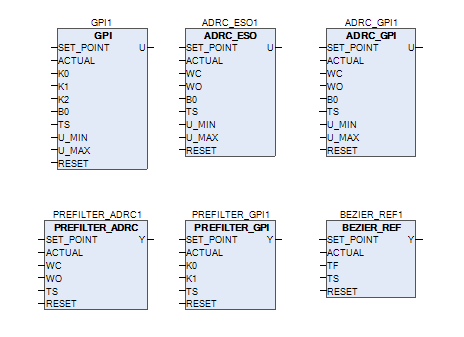
\includegraphics[width=0.68\textwidth]{codesys_bloques.png}
  \caption[Instancias de los bloques en CODESYS]{Instancias de los bloques de función en CODESYS.}
  \label{fig:plc_codesys}
\end{figure}

Para probar el lazo completo se conectó cada combinación de consigna y controlador al bloque
\texttt{PLANT}, configurado como la planta de diseño, $\tau = 1200$~s y $k_{dc} = 0{,}05$~mg/(L$\cdot$\%),
y con la misma sintonía de las secciones anteriores: $\omega_c = 4/\tau$, $\omega_o = 5\,\omega_c$,
$b_0 = k_{dc}/\tau$ y $T_s = 50$~ms. La
Figura~\ref{fig:plc_en_linea} muestra dos de estas pruebas en línea, ya en régimen: la orden de
$40~\%$ sostiene $2$~mg/L y la de $44~\%$ sostiene $2{,}2$~mg/L, que es lo que da $k_{dc}$. Así se valida que el comportamiento sea el
correspondiente.

\begin{figure}[H]
  \centering
  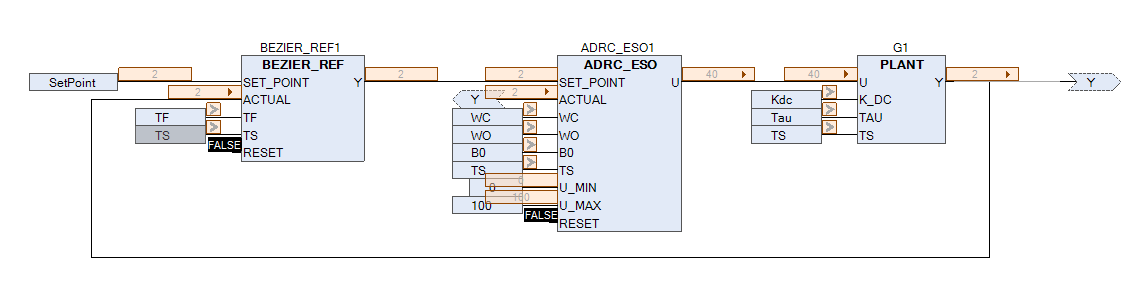
\includegraphics[width=\textwidth]{codesys_bezier_eso_en_linea.png}\\[6pt]
  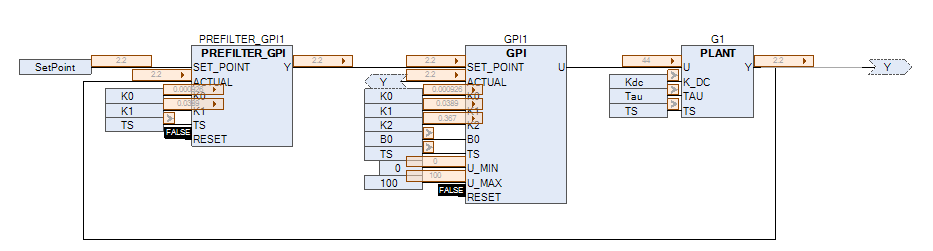
\includegraphics[width=\textwidth]{codesys_prefilter_gpi_en_linea.png}
  \caption[Lazos en línea en CODESYS]{Lazos en línea con el bloque \texttt{PLANT}. Arriba, \texttt{BEZIER\_REF} y \texttt{ADRC\_ESO} con consigna de $2$~mg/L; abajo,
    \texttt{PREFILTER\_GPI} y \texttt{GPI} con consigna de $2{,}2$~mg/L.}
  \label{fig:plc_en_linea}
\end{figure}

La Figura~\ref{fig:plc_trazas} muestra las trazas registradas por el PLC en dos corridas, con cambios
de consigna de $0$ a $2$~mg/L y de $2$ a $2{,}2$~mg/L, y la Tabla~\ref{tab:plc_trazas} resume la
información. Con Bézier se usó $t_f = 2400$~s para el primer cambio de referencia y $t_f = 1200$~s
para el segundo. La curva de Bézier no lleva el control a la saturación en el primer escalón, que era
el que requería mayor esfuerzo, y deja un sobrepico de $4{,}4~\%$ en el segundo, porque el cero sigue
en el lazo. Aun así, no se pierde robustez ni rechazo, ya que la curva de Bézier solo ayuda a que la
salida llegue a la referencia suavemente. El prefiltro no tiene sobrepico en ninguno de los dos, pero en el escalón
grande la orden llega a $100~\%$ durante $30{,}6$~s. En el escalón pequeño, el prefiltro con el ADRC se
asienta en $24{,}5$~min con una orden máxima de $50{,}1~\%$, prácticamente los mismos valores de la
Tabla~\ref{tab:disc_prefiltro_indices} para $T_s = 50$~ms sin retardo.

\begin{figure}[H]
  \centering
  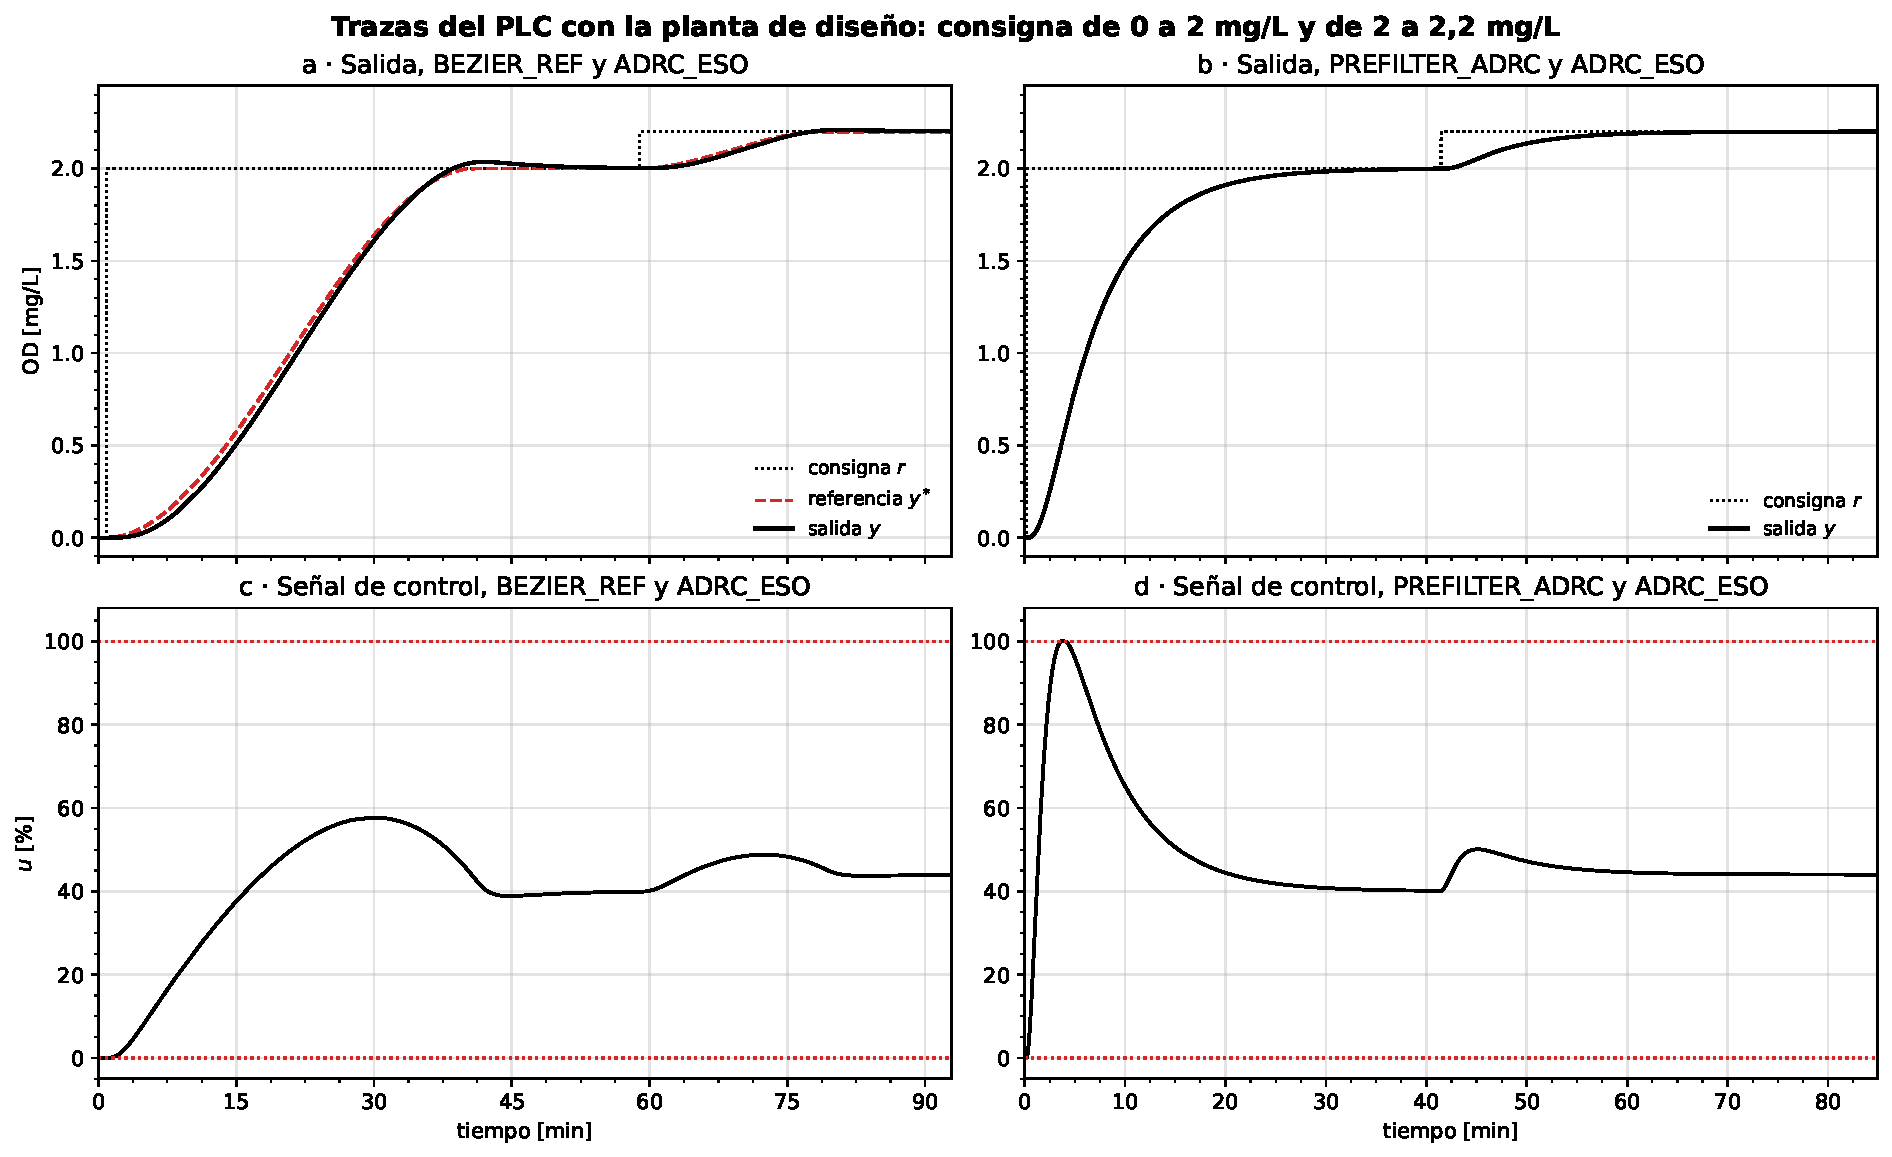
\includegraphics[width=\textwidth]{plc_trazas.pdf}
  \caption[Trazas del PLC con Bézier y con prefiltro]{Trazas registradas por el PLC con el bloque
    \texttt{PLANT} configurado como la planta de diseño. (a) y (c) \texttt{BEZIER\_REF} con
    \texttt{ADRC\_ESO}. (b) y (d) \texttt{PREFILTER\_ADRC} con \texttt{ADRC\_ESO}.}
  \label{fig:plc_trazas}
\end{figure}

\begin{table}[H]
\centering
\caption[Indicadores de las trazas del PLC]{Indicadores de las trazas de la
  Figura~\ref{fig:plc_trazas}, medidos desde cada cambio de consigna.}
\label{tab:plc_trazas}
\renewcommand{\arraystretch}{1.2}
\begin{tabular}{llccc}
\toprule
\textbf{Lazo} & \textbf{Consigna [mg/L]} & \textbf{Sobrepico} & \textbf{$t_s$ ($2~\%$)} & \textbf{$u$ máxima} \\
\midrule
\texttt{BEZIER\_REF} y \texttt{ADRC\_ESO} & $0 \to 2$ & $1{,}8~\%$ & $36{,}3$~min & $57{,}7~\%$ \\
 & $2 \to 2{,}2$ & $4{,}4~\%$ & $27{,}4$~min & $48{,}8~\%$ \\
\addlinespace
\texttt{PREFILTER\_ADRC} y \texttt{ADRC\_ESO} & $0 \to 2$ & $0~\%$ & $24{,}4$~min & $100~\%$ \\
 & $2 \to 2{,}2$ & $0~\%$ & $24{,}5$~min & $50{,}1~\%$ \\
\bottomrule
\end{tabular}
\end{table}



%--------------------------------------------------------------------
\section{Resumen: recetas de implementación}
\label{sec:impl_resumen}

En esta sección se organiza lo desarrollado para implementar el ADRC y el GPI dentro de un dispositivo
digital como un PLC, en cuatro recetas: el ADRC con observador de estado extendido a nivel general, el
GPI, los aspectos prácticos de implementación y, por último, la implementación en el PLC. Cada paso
dice qué hacer y remite a la ecuación o la sección donde está el detalle.

\subsection{Implementación del ADRC con observador de estado extendido: caso general}

\begin{recuadro}{Receta 1}
\begin{enumerate}\setlength{\itemsep}{2pt}
  \item \textbf{Modelo de la planta.} Con un experimento cerca del punto de operación
  (Figura~\ref{fig:ident_escalon_ref}) se mide cuánto cambia la salida ante un cambio en la entrada, y
  de ahí se hallan el orden $n$, la ganancia $k_{dc}$ y la constante de tiempo $\tau$ o el ancho de
  banda. Con eso se obtiene $b_0$, que para primer orden es $k_{dc}/\tau$ \eqref{eq:car_b0} y para
  otros órdenes sale de \cite[tabla~3.1]{herbst2024adrc}. Luego se reescribe la planta sobre el error:
  con $u_0 = b_0\,u$, la dinámica del error queda como una cadena de $n$ integradores excitada por
  $u_0 + \xi$ \eqref{eq:error_norm}.
  \item \textbf{Perturbación.} Se elige el modelo interno según la señal que se desea rechazar:
  escalones $1/s$ ($m = 1$), rampas $1/s^2$ ($m = 2$) o polinomios de mayor grado. Las perturbaciones
  que no siguen ese modelo también se rechazan, en la medida en que lo permita el ancho de banda del
  observador.
  \item \textbf{Sistema aumentado y observador.} Se juntan la cadena de integradores y el modelo
  interno en un solo sistema de orden $n + m$ \eqref{eq:aumentado}, cuyos estados son el error, sus
  derivadas y la perturbación con sus derivadas \eqref{eq:aumentado_matrices}. Sobre él se arma el
  observador \eqref{eq:observador}, que recibe el error medido y la orden $u_0$ y estima todos esos
  estados \eqref{eq:observador_matrices}.
  \item \textbf{Sintonía del controlador.} Se necesitan $n$ ganancias, $k_{p_1}, \dots, k_{p_n}$
  (Sección~\ref{subsec:ley}). Se pueden ubicar los polos donde se quiera con la fórmula de Ackermann
  \eqref{eq:ackermann_K}, o ponerlos todos en $-\omega_c$ con la sintonía por ancho de banda
  \eqref{eq:sintonia_l}, donde $\omega_c$ define qué tan rápido llega el sistema al estacionario. En
  la planta se eligió $\omega_c = 4/\tau$, cuatro veces más rápido que la planta en lazo abierto, que
  es la dinámica final que queda.
  \item \textbf{Sintonía del observador.} Se necesitan $n + m$ ganancias, que estiman tanto los
  estados de la planta como la perturbación: con Ackermann para el observador \eqref{eq:ackermann_L},
  o por ancho de banda \eqref{eq:sintonia_l}, con todos los polos en $-\omega_o$, donde $\omega_o$
  está entre $3$ y $10$ veces $\omega_c$ \cite[sec.~3.3]{herbst2024adrc}. En la planta se eligió
  $\omega_o = 5\,\omega_c$.
\end{enumerate}
\end{recuadro}

\subsection{Implementación del GPI}

\begin{recuadro}{Receta 2}
\begin{enumerate}\setlength{\itemsep}{2pt}
  \item \textbf{Modelo de la planta.} Igual que en el ADRC: el orden $n$ y la ganancia $b_0$
  \eqref{eq:car_b0}, con el mismo experimento cerca del punto de operación.
  \item \textbf{Perturbación e integradores.} Se elige la señal que se quiere rechazar, es decir, el
  modelo interno $D_A = s^m$ del lazo cerrado escrito como fracción \eqref{eq:gpi_lazo_general}. El
  controlador se construye solo con integrales del error y de la señal de control, reconstruyendo el
  error en vez de observarlo (Sección~\ref{subsec:gpi_integradores}); para $n = m = 1$ queda un PI con
  un polo adicional, dado por el filtro \eqref{eq:gpi_ley}, y la Tabla~\ref{tab:gpi_conteo} resume los
  controladores que se obtienen según $n$ y $m$.
  \item \textbf{Sintonización.} Las ganancias $k_2$, $k_1$ y $k_0$ son los coeficientes del polinomio
  característico \eqref{eq:gpi_producto}, así que con ellas se decide la dinámica del error de
  seguimiento: los polos del lazo cerrado y del rechazo de la perturbación \eqref{eq:gpi_producto_S}.
  Se pueden ajustar como un PI con filtro, con $k_1/b_0$ como ganancia proporcional, $k_0/b_0$ como
  integral y $k_2$ como polo del filtro \eqref{eq:gpi_pi_filtro}, o con el enfoque del ADRC: los
  polos en $-\omega_c$ y $-\omega_o$ dan un polinomio cuyos coeficientes son $k_0$, $k_1$ y $k_2$
  \eqref{eq:eso2gpi}.
\end{enumerate}
\end{recuadro}

\subsection{Aspectos prácticos de implementación}

\begin{recuadro}{Receta 3}
\begin{enumerate}\setlength{\itemsep}{2pt}
  \item \textbf{Manejo de la saturación.} Al observador del ESO le entra la orden aplicada
  $u_{\mathrm{sat}}$ y no la pedida $u$ (Figura~\ref{fig:simulink_eso}); con eso el ADRC ya tiene
  \emph{anti-windup}. El GPI usa el esquema de saturación de la
  Figura~\ref{fig:simulink_gpi}. Al elegir $\omega_c$, validar ante una entrada paso que $u$ no se
  sature cerca del punto de operación, porque si se satura no se obtiene la dinámica esperada.
  \item \textbf{Acondicionamiento de la referencia.} Tanto en el ESO como en el GPI se suaviza la
  consigna para evitar el pico de $u$ y el sobrepico que produce el cero de $y/r$: con un polinomio de
  Bézier de grado $3$, eligiendo el tiempo final y la consigna (Sección~\ref{subsec:bz_planificacion}),
  o con un prefiltro de primer orden con el polo en el cero del lazo cerrado
  (Figura~\ref{fig:pref_lazo}).
  \item \textbf{Ruido.} El ESO y el GPI comparten la misma función de transferencia, que es
  estrictamente propia, así que ya filtran el ruido de alta frecuencia sin filtros adicionales. Para
  dejar pasar menos ruido a la señal de control se disminuye el ancho de banda del observador, $\omega_o$
  (Sección~\ref{sec:impl_ruido} y Figura~\ref{fig:adrc_gang_kESO}(h)): entre más alto, mejor rechazo
  de la perturbación, pero más ruido.
  \item \textbf{Discretización.} El observador del ESO conserva su estructura
  \eqref{eq:disc_observador}; solo cambian las matrices del sistema aumentado, donde los integradores
  pasan a discreto con ZOH \eqref{eq:disc_matrices} (para $n = m = 1$, en la
  Tabla~\ref{tab:disc_matrices}). El GPI se discretiza bloque por bloque con Tustin
  \eqref{eq:disc_gpi_tf}. En los dos casos, muestrear al menos a $10$ veces el ancho de banda del lazo
  cerrado, o $10$ veces el polo más rápido, que es el del observador, y, como recomendación, por lo menos $20$ veces: entre más
  rápido el muestreo, más se parece el resultado al continuo.
  \item \textbf{Retardo.} Si se conoce el retardo $\theta$, se sincroniza el observador con la planta
  retrasando $n_d \approx \theta/T_s$ muestras la orden que le entra \eqref{eq:disc_retardo}; otra forma es aumentar el margen
  de fase, disminuyendo $\omega_c$, y suavizar la respuesta.
  \item \textbf{Implementación.} Para el ESO se usa la realización con dos retardos de la
  Figura~\ref{fig:adrc_discreto_retardos}; si se quiere sintonizar con anchos de banda,
  $\mathbf{K}_d$ y $\mathbf{L}_d$ se calculan desde $\omega_c$ y $\omega_o$
  \eqref{eq:disc_ganancias_wc_wo} al inicio del algoritmo. Para el GPI se usa la forma directa I de la
  Figura~\ref{fig:disc_formas_directas}, con los coeficientes de la Tabla~\ref{tab:disc_gpi_coef}, sea
  con $k_0$, $k_1$ y $k_2$, tipo PI con filtro, o con anchos de banda.
\end{enumerate}
\end{recuadro}

\subsection{Implementación en el PLC}

\begin{recuadro}{Receta 4}
Aquí ya no se usa el caso general, sino solo lo específico de la planta, $n = m = 1$: los esquemas de
las Figuras~\ref{fig:adrc_discreto_retardos} y \ref{fig:disc_formas_directas}, con las ganancias de las
Tablas~\ref{tab:disc_matrices} y \ref{tab:disc_gpi_coef}, en texto estructurado
(Sección~\ref{sec:impl_plc}); el código se puede revisar en el repositorio del Anexo~\ref{anx:st}.
\begin{enumerate}\setlength{\itemsep}{2pt}
  \item \textbf{Tiempo de muestreo.} Es el ciclo de la tarea en la que se ejecuta el bloque. Se
  recomienda una tarea dedicada solo al controlador. La frecuencia con la que se discretiza la
  variable del proceso sí debe ser más rápida que la de ejecución del controlador, para tener listos
  los datos antes de que el controlador inicie su maniobra.
  \item \textbf{Modelo de la planta.} Con el mismo experimento cerca del punto de operación, cuánto
  cambia la salida al cambiar la entrada, se obtienen $k_{dc}$ y $\tau$, y con ellos
  $b_0 = k_{dc}/\tau$ \eqref{eq:car_b0}.
  \item \textbf{Sintonía del controlador.} $\omega_c = 4/\tau$, cuatro veces más rápido que la planta
  en lazo abierto; se puede modificar según la velocidad de respuesta deseada, siempre que el sistema
  no se sature con cambios de referencia cerca del punto de operación.
  \item \textbf{Sintonía del observador.} En el ADRC, $\omega_o$ entre $3$ y $10$ veces $\omega_c$,
  según qué tanto se quiera rechazar la perturbación. Para este caso, con $\omega_o = 5\,\omega_c$
  queda por debajo de $\omega_o$ el $99~\%$ de la energía de la perturbación; el tope lo pone el ruido,
  es decir, qué tanto ruido admisible deja pasar el observador a la señal de control. El GPI se puede sintonizar como un PI clásico
  con \emph{pole placement}, y manejar el cero del numerador con el prefiltro o con Bézier para
  reducir el esfuerzo de control.
  \item \textbf{Referencia con Bézier.} Al bloque \texttt{BEZIER\_REF} se le pasa el tiempo final
  $t_f$. Por dentro usa el polinomio de grado $3$ \eqref{eq:bz_pol}, con coeficientes que se
  recalculan desde el estado de la referencia cada vez que cambia la consigna \eqref{eq:bz_sistema_c},
  y lo evalúa en forma compacta con el tiempo normalizado \eqref{eq:bz_horner}
  (Sección~\ref{subsec:bz_replanificacion}).
  \item \textbf{Referencia con prefiltro.} Según el enfoque, a \texttt{PREFILTER\_ADRC} se le pasan
  $\omega_c$ y $\omega_o$, y a \texttt{PREFILTER\_GPI}, $k_0$ y $k_1$
  (Tablas~\ref{tab:plc_prefilter_adrc} y \ref{tab:plc_prefilter_gpi}). Por dentro usan el prefiltro
  discretizado con Tustin \eqref{eq:disc_pref_tf}, con las ganancias de la Tabla~\ref{tab:disc_pref}.
\end{enumerate}
\end{recuadro}

% ============================================================================
%  Capítulo 6 - Comparación PID ISA contra ADRC
% ============================================================================
\chapter{Comparación PID ISA contra ADRC}
\label{cap:comparacion_pid}
En este capítulo se compara un PID ISA ideal, con filtro en la acción derivativa, con el ADRC de los
capítulos anteriores, bajo un mismo grado de robustez, y se mide su desempeño con métricas clásicas,
para ver en qué casos el ADRC puede llegar a ser más beneficioso de implementar que el PID y qué
ventajas y desventajas tiene frente a un PID convencional. Para ello también se usa la perturbación
total medida en M2 en la Sección~\ref{sec:ident_perturbacion}.
%--------------------------------------------------------------------
\section{PID con misma robustez}
\label{sec:pid_robustez}

Se usa un PID ISA ideal con filtro en la acción derivativa, que actúa sobre el mismo error que el ADRC,
$e = r - y = -e_y$:
\begin{equation}
C_{PID}(s) = K_p\left(1 + \frac{1}{T_i\,s} + \frac{T_d\,s}{1 + \dfrac{T_d}{N}\,s}\right),
\label{eq:pid_isa}
\end{equation}
con $K_p$ la ganancia proporcional, $T_i$ el tiempo integral, $T_d$ el tiempo
derivativo y $N$ el que fija el filtro de la derivada.

\paragraph{Sintonía.} El PID se sintoniza en dos pasos. Primero se elige $K_p$ para que la señal de
control no salte de forma exagerada en el cambio de consigna. Ante un escalón $\Delta r$, la acción resultante es $K_p\,(1 + N)\,\Delta r$. Se busca un salto de cerca de $40~\%$ ante el
escalón de $0{,}2$~mg/L, de $40$ a $80~\%$, el mismo pico de la señal de control del ADRC. Con el valor
típico $N = 10$ queda un $K_p$ pequeño: la acción proporcional, que es la que mueve la salida al inicio
y rechaza las perturbaciones, sería tan débil que el controlador quedaría casi sin fuerza para rechazar
la perturbación y muy lento. Por eso se usa $N = 2$, que deja más acción proporcional para el mismo
salto. Luego se ajustan las acciones integral y derivativa para que el PID tenga, sin retardo, la misma
sensibilidad máxima $M_s$ que el ADRC. El retardo $\theta = 50$~s solo se usa para evaluar. Resulta
\begin{equation}
K_p = 66{,}7~\%/(\mathrm{mg/L}),
\qquad
T_i = 160{,}9~\mathrm{s},
\qquad
T_d = 40{,}2~\mathrm{s},
\qquad
N = 2 .
\label{eq:pid_ganancias}
\end{equation}
Con la misma $M_s$, el PID queda con un ancho de banda menor que el del ADRC, porque el salto inicial
limita su ganancia, y en la Figura~\ref{fig:pid_adrc_sensibilidad}(a) se ve que su pico de sensibilidad
está en una frecuencia mucho más baja. Es decir, para esta misma configuración el ADRC puede rechazar
perturbaciones de frecuencias mucho más altas que el PID. Con $\theta = 50$~s los dos quedan con casi el
mismo margen de fase; el PID pierde menos robustez al usar la planta con retardo y tiene un mayor margen
de ganancia, pero es más lento (Tabla~\ref{tab:pid_robustez} y Figura~\ref{fig:pid_adrc_escalon}).

\begin{table}[H]
\centering
\caption[Robustez del ADRC y del PID ISA]{Robustez del ADRC y del PID ISA (Tabla~\ref{tab:metricas_robustez}), sin
  retardo (diseño) y con $\theta = 50$~s (evaluación).}
\label{tab:pid_robustez}
\renewcommand{\arraystretch}{1.3}
\begin{tabular}{llccccc}
\toprule
 & $\boldsymbol{\theta}$ & $\boldsymbol{M_s}$ & $\boldsymbol{M_t}$ &
 \textbf{MF} & \textbf{MG} & $\boldsymbol{\omega_{BW}}$ \textbf{[rad/h]} \\
\midrule
ADRC & 0     & 1,202 & 1,100 & $65{,}8^{\circ}$ & $\infty$ & 56,4 \\
PID  & 0     & 1,202 & 1,418 & $50{,}0^{\circ}$ & $\infty$ & 21,2 \\
\midrule
ADRC & 50~s  & 2,318 & 1,700 & $36{,}0^{\circ}$ & 2,12     & 79,0 \\
PID  & 50~s  & 1,585 & 1,709 & $37{,}5^{\circ}$ & 7,37     & 23,8 \\
\bottomrule
\end{tabular}
\end{table}

\begin{figure}[H]
  \centering
  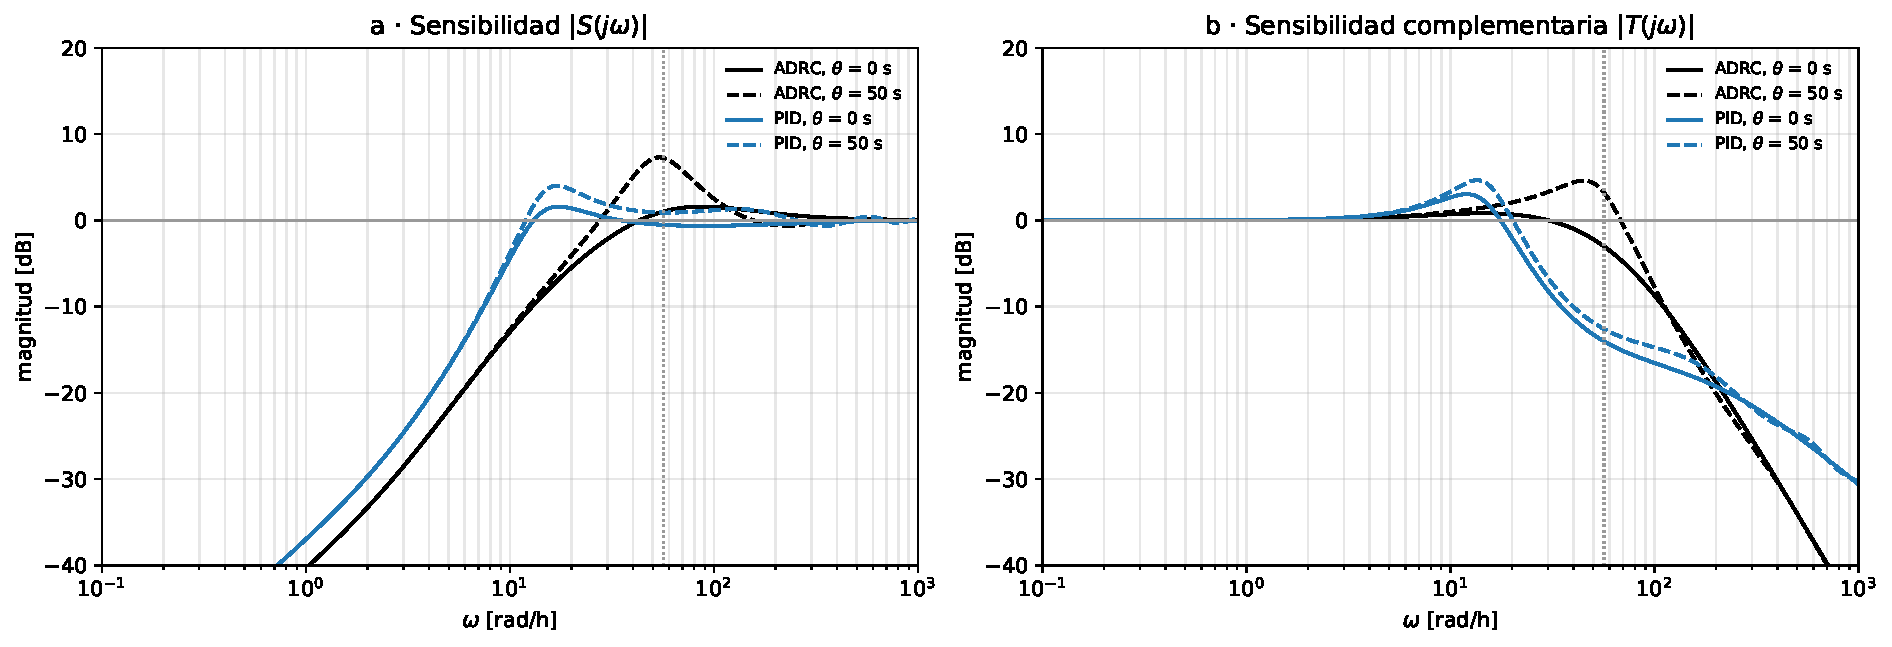
\includegraphics[width=\textwidth]{pid_adrc_sensibilidad.pdf}
  \caption[Sensibilidad del ADRC y del PID ISA]{Sensibilidad del ADRC y del PID
    ISA sin retardo (continua) y con $\theta = 50$~s (discontinua): (a)
    $|S(j\omega)|$ y (b) $|T(j\omega)|$. La vertical punteada marca
    el $\omega_{BW}$ del ADRC.}
  \label{fig:pid_adrc_sensibilidad}
\end{figure}

\paragraph{Escalón de consigna.} Se aplica el cambio de $2{,}0$ a
$2{,}2$~mg/L, sin retardo, que es el caso de diseño, y con $\theta = 50$~s
(Figura~\ref{fig:pid_adrc_escalon}), con el ruido del sensor
de la Sección~\ref{sec:ident_ruido} ($\sigma = 0{,}0011$~mg/L, blanco, a 50~ms)
sumado a la medida. El soplador se limita entre $0$ y $100~\%$: el ADRC
realimenta $b_0\,u_{\mathrm{sat}}$ al observador, y el PID usa el mismo esquema de anti-\emph{windup}
que el GPI \eqref{eq:aw_gpi} \cite[ec.~19.3]{levine2011handbook}. Con
este escalón ninguno de los dos llega al límite del soplador: el pico del ADRC es
de $80~\%$ sin retardo y de $93~\%$ con $\theta = 50$~s, y el del PID es de
$80~\%$ en los dos casos. La Tabla~\ref{tab:pid_escalon} reúne las métricas de la
Tabla~\ref{tab:metricas}: IAE, ITAE, $M_p$, $t_s$, los valores extremos de $u$, la variación total TV y
$\sigma_u$, esta última con el sistema en estacionario.

\begin{figure}[H]
  \centering
  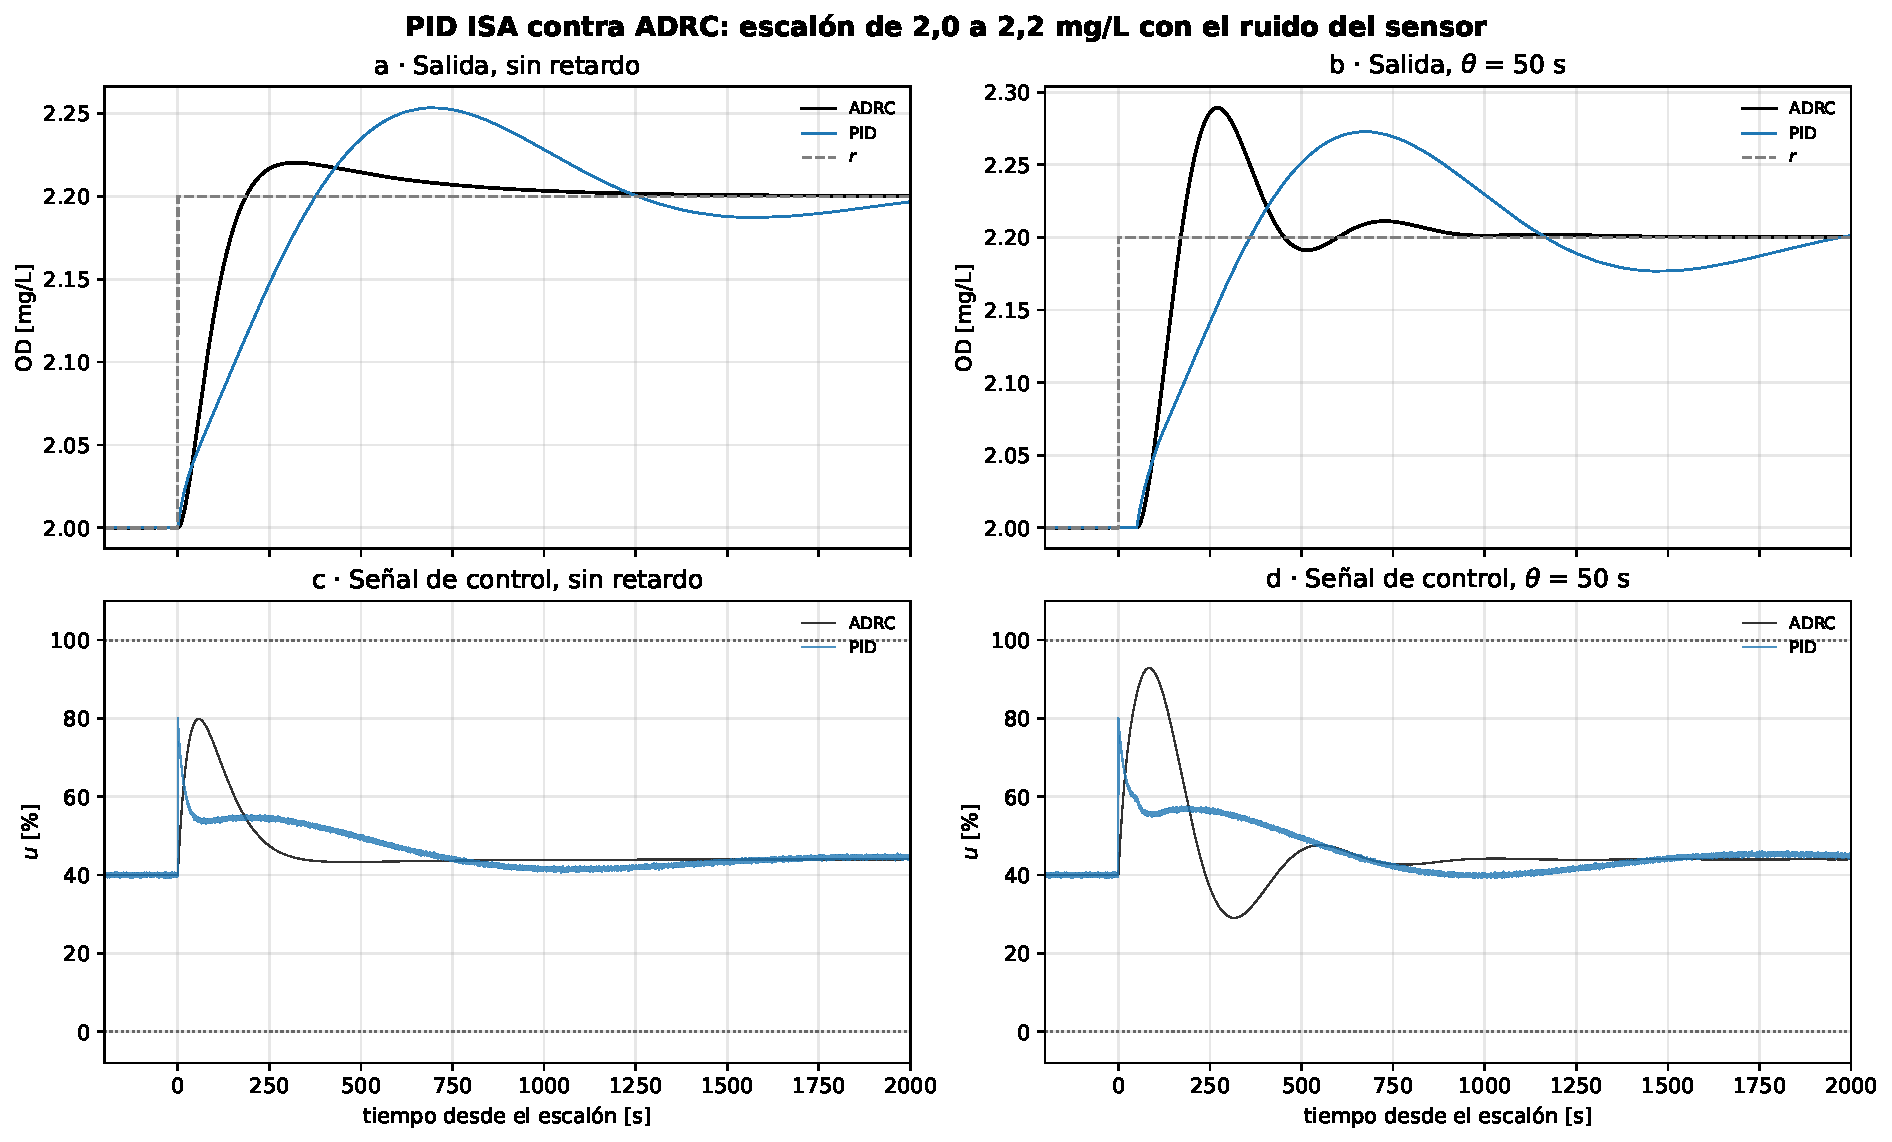
\includegraphics[width=\textwidth]{pid_adrc_escalon.pdf}
  \caption[PID ISA contra ADRC: escalón de consigna]{PID ISA contra ADRC en el escalón de $2{,}0$ a
    $2{,}2$~mg/L con el ruido del sensor y el soplador limitado entre $0$ y $100~\%$. (a) y (c) Salida y
    señal de control sin retardo; (b) y (d) con $\theta = 50$~s.}
  \label{fig:pid_adrc_escalon}
\end{figure}

\begin{table}[H]
\centering
\caption[Índices del escalón de consigna]{Índices del escalón de $2{,}0$ a
  $2{,}2$~mg/L sin retardo y con $\theta = 50$~s.}
\label{tab:pid_escalon}
\renewcommand{\arraystretch}{1.3}
\resizebox{\textwidth}{!}{%
\begin{tabular}{llccccccc|cc}
\toprule
 & & \multicolumn{7}{c|}{\textbf{Sin ruido}} & \multicolumn{2}{c}{\textbf{Con ruido}} \\
 & $\boldsymbol{\theta}$ & \textbf{IAE} & \textbf{ITAE} & $\boldsymbol{M_p}$ & $\boldsymbol{t_s}$ &
 $\boldsymbol{u_{\max}}$ & $\boldsymbol{u_{\min}}$ &
 \textbf{TV} & $\boldsymbol{\sigma_u}$ & \textbf{TV} \\
 & [s] & [mg$\cdot$s/L] & [mg$\cdot$s$^2$/L] & [\%] & [min] & [\%] & [\%] & [\%] & [\%] & [\%] \\
\midrule
ADRC & 0  & 26,9 & 6\,909  & 10,2 & 15,7   & 79,8 & 40,0 & 77  & 0,009 & 96 \\
PID  & 0  & 69,2 & 40\,127 & 26,7 & 32,9   & 80,0 & 40,0 & 84  & 0,220 & 13\,876 \\
\midrule
ADRC & 50 & 42,7 & 9\,308  & 44,6 & 14,7   & 92,8 & 29,0 & 142 & 0,010 & 158 \\
PID  & 50 & 88,4 & 56\,567 & 36,4 & 42,7   & 80,0 & 39,9 & 90  & 0,220 & 13\,873 \\
\bottomrule
\end{tabular}%
}
\end{table}

Sin retardo, con la misma sensibilidad y sin que la señal de control llegue a la saturación, el PID
es un poco más lento y tiene un sobrepico más grande, es decir, un desempeño algo peor que el del ADRC
(Figura~\ref{fig:pid_adrc_escalon}(a)). Además, en la
Figura~\ref{fig:pid_adrc_escalon}(c) ya se alcanza a ver el ruido que el PID deja pasar a la
señal de control, porque es bipropio (Sección~\ref{sec:impl_ruido}), mientras que el ADRC casi no lo deja
pasar. Cuando se introduce el retardo (Figura~\ref{fig:pid_adrc_escalon}(b) y (d)), el ADRC empieza a oscilar; el
PID, como ya era lento, no oscila tanto, pero tampoco tiene un buen desempeño y tarda mucho más en
asentarse. De hecho, con el retardo de la planta los dos tienen casi el mismo margen de fase
(Tabla~\ref{tab:pid_robustez}), pero el PID tiene un mayor margen de ganancia, pagando con un sistema
más lento. Ahora bien, el desempeño del ADRC es mejor, con un IAE y un ITAE mucho menores, tanto sin
retardo como con retardo y con la misma $M_s$; con retardo el PID queda con mejor $M_s$. El otro tema es el ruido: en la Figura~\ref{fig:pid_adrc_escalon} y en la
Tabla~\ref{tab:pid_escalon} se ve que el ruido que alcanza a pasar a la señal de control es mucho mayor
en el PID que en el ADRC.

%--------------------------------------------------------------------
\section{Perturbación de entrada}
\label{sec:pid_perturbacion_escalon}

Con el sistema en estacionario en $2{,}0$~mg/L entra una perturbación de entrada $\varepsilon = -15~\%$, una
pérdida de eficiencia del soplador, sin retardo y con $\theta = 50$~s
(Figura~\ref{fig:pid_adrc_perturbacion_escalon}). La Tabla~\ref{tab:pid_pert_escalon} reúne el IAE, la
caída máxima del OD y cuánto se pasa la salida por encima de la consigna al recuperarse, en porcentaje
de la caída (Tabla~\ref{tab:metricas}).

\begin{figure}[H]
  \centering
  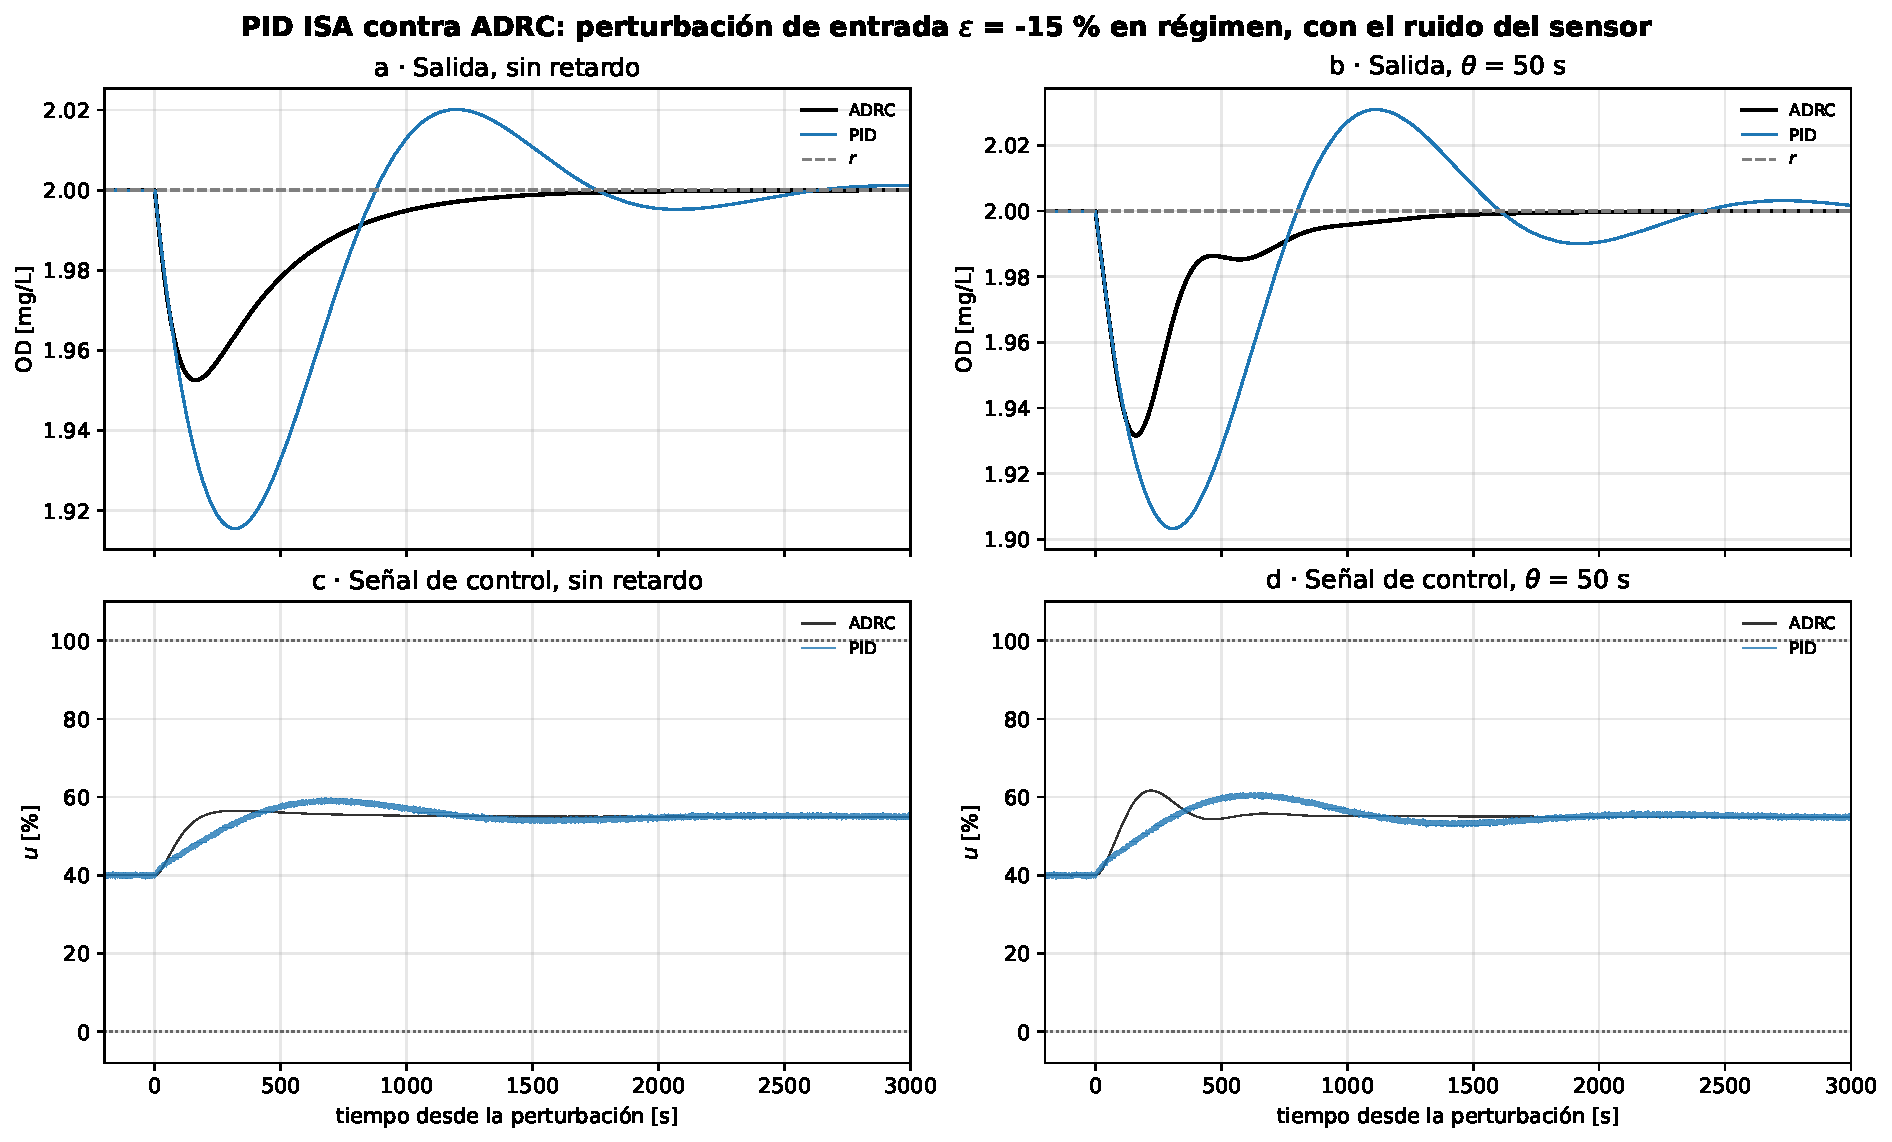
\includegraphics[width=\textwidth]{pid_adrc_perturbacion_escalon.pdf}
  \caption[PID ISA contra ADRC: perturbación de entrada]{PID ISA contra ADRC ante una perturbación de
    entrada $\varepsilon = -15~\%$ con el sistema en estacionario en $2{,}0$~mg/L, el ruido del sensor y el soplador
    limitado entre $0$ y $100~\%$. (a) y (c) Salida y señal de control sin retardo; (b) y (d) con
    $\theta = 50$~s.}
  \label{fig:pid_adrc_perturbacion_escalon}
\end{figure}

\begin{table}[H]
\centering
\caption[Índices de la perturbación de entrada]{Índices de la perturbación de entrada
  $\varepsilon = -15~\%$ de la Figura~\ref{fig:pid_adrc_perturbacion_escalon}, medidos sin ruido desde
  que entra la perturbación.}
\label{tab:pid_pert_escalon}
\renewcommand{\arraystretch}{1.3}
\begin{tabular}{llcccc}
\toprule
 & $\boldsymbol{\theta}$ & \textbf{IAE} & \textbf{Caída máxima} & \textbf{Sobrepaso} & $\boldsymbol{u_{\max}}$ \\
 & [s] & [mg$\cdot$s/L] & [mg/L] & [\% de la caída] & [\%] \\
\midrule
ADRC & 0  & 24,8 & 0,047 & 0    & 56,5 \\
PID  & 0  & 58,8 & 0,085 & 23,9 & 59,0 \\
\midrule
ADRC & 50 & 24,8 & 0,068 & 0    & 61,7 \\
PID  & 50 & 70,2 & 0,097 & 32,0 & 60,5 \\
\bottomrule
\end{tabular}
\end{table}

En la perturbación de entrada (Figura~\ref{fig:pid_adrc_perturbacion_escalon}) se sigue viendo que el
ADRC tiene un mejor rechazo y sin tantas oscilaciones: cae menos y vuelve a la consigna sin pasarse,
porque el observador estima la perturbación y la orden la compensa directamente. El PID cae casi el
doble, es decir, le cuesta más rechazar la perturbación, y al recuperarse se pasa con un sobrepico más
grande; su señal de control se recupera más lento, aunque su pico es casi el mismo que el del ADRC.
Para este caso el IAE es mejor en el ADRC, lo que se traduce en un mejor desempeño.



%--------------------------------------------------------------------
\section{Perturbación medida}
\label{sec:pid_perturbacion}

La perturbación total medida en M2 (Sección~\ref{sec:ident_perturbacion}), $\bar{\xi}$ en
mg/(L$\cdot$h), entra como perturbación de entrada en \% de $u$; la usaremos para validar el
desempeño que tienen los controladores:
\begin{equation}
\varepsilon(t) = \frac{\bar{\xi}(t)/3600 + y_{\mathrm{med}}(t)/\tau}{b_0} ,
\label{eq:pid_eps}
\end{equation}
con $y_{\mathrm{med}}$ el OD medido en la planta. Se toman las 12~h de la
Figura~\ref{fig:ident_perturbacion}, en las que la perturbación primero deja trabajar al
soplador, luego lo satura y después cede, con $\theta = 50$~s y el soplador limitado entre $0$ y $100~\%$,
con el mismo manejo de la saturación: arranque desde
$0$~mg/L, con el soplador apagado, hasta 2,0~mg/L, cambio a 2,2~mg/L a las
4~h y a 1,8~mg/L a las 8~h. Se corre con el ruido del sensor, y se
dibuja también la perturbación que estima el observador del ADRC, llevada a
las mismas unidades que $\bar{\xi}$ (Figura~\ref{fig:pid_adrc_perturbacion}). La perturbación que se dibuja es
$\bar{\xi}$, la que actúa sobre la salida, y por eso no tiene los cambios de consigna; el observador, en
cambio, trabaja sobre el error y estima $\xi = \bar{\xi} - \dot{y^*}$, de modo que en su estimación aparecen
picos a las 4 y a las 8~h, justo en los cambios de consigna. Los resultados de las métricas se registran en la
Tabla~\ref{tab:pid_cambios}.

\begin{figure}[H]
  \centering
  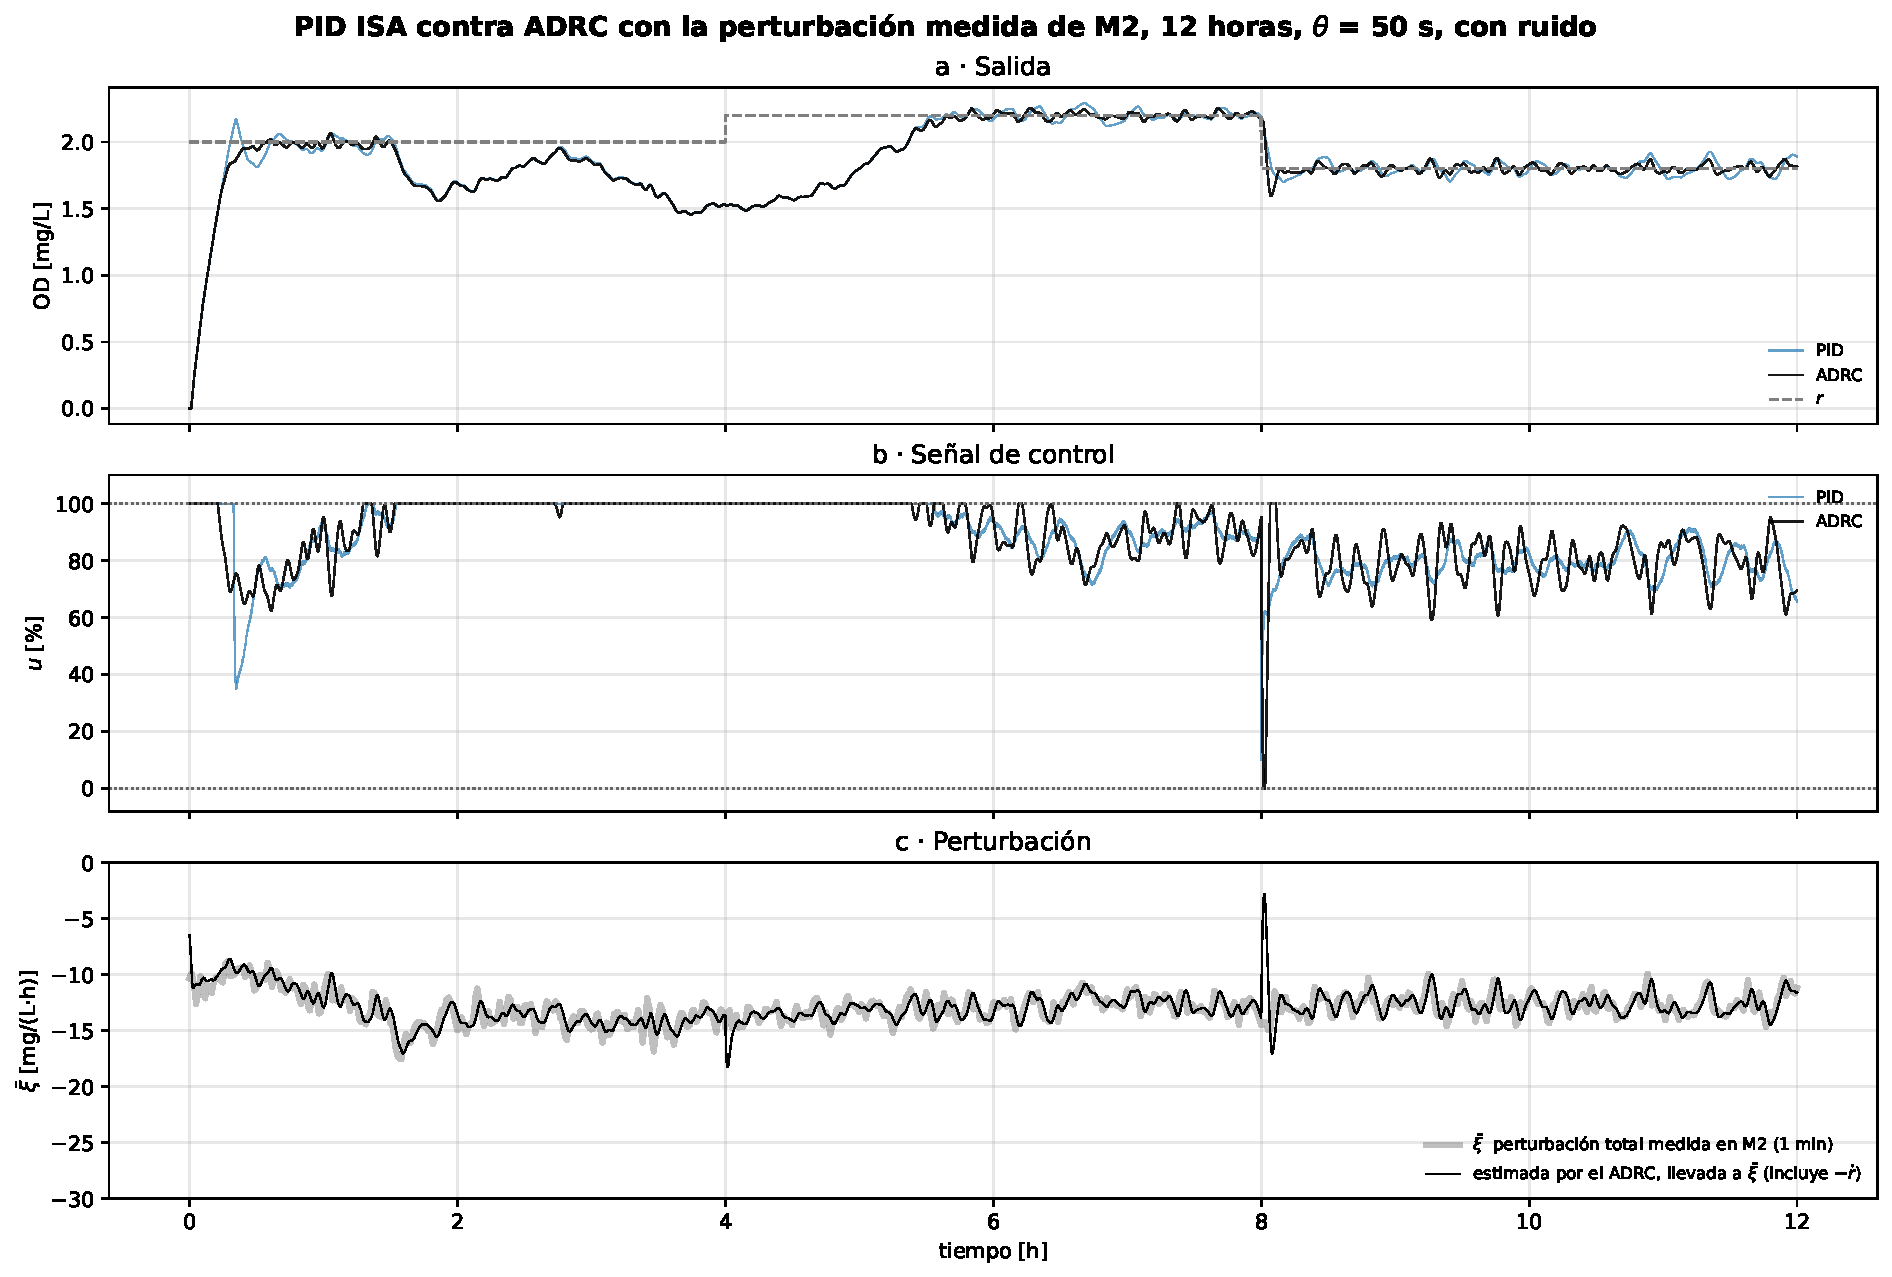
\includegraphics[width=\textwidth]{pid_adrc_perturbacion.pdf}
  \caption[PID ISA contra ADRC con la perturbación medida]{PID ISA contra
    ADRC con las 12~h de la perturbación medida en M2 de la Figura~\ref{fig:ident_perturbacion}, arranque desde
    $0$~mg/L y cambios de consigna a las 4 y a las 8~h, con $\theta = 50$~s y
    el soplador limitado entre $0$ y $100~\%$, con el ruido del sensor.
    (a) Salida. (b) Señal de control. (c) Perturbación total sobre la salida $\bar{\xi}$, medida y
    estimada por el observador del ADRC.}
  \label{fig:pid_adrc_perturbacion}
\end{figure}

\begin{table}[H]
\centering
\caption[Índices por cambio de consigna con la perturbación medida]{Índices
  de cada cambio de consigna con la perturbación medida, en una ventana de
  2~h desde el cambio. El IAE incluye el efecto de la perturbación en esa
  ventana.}
\label{tab:pid_cambios}
\renewcommand{\arraystretch}{1.3}
\resizebox{\textwidth}{!}{%
\begin{tabular}{lccccccc}
\toprule
 & & \multicolumn{2}{c}{\textbf{IAE sin ruido}} & \multicolumn{2}{c}{\textbf{IAE con ruido}} & \multicolumn{2}{c}{$\boldsymbol{M_p}$ \textbf{sin ruido}} \\
 & & \multicolumn{2}{c}{[mg$\cdot$s/L]} & \multicolumn{2}{c}{[mg$\cdot$s/L]} & \multicolumn{2}{c}{[\%]} \\
\cmidrule(lr){3-4} \cmidrule(lr){5-6} \cmidrule(lr){7-8}
\textbf{Cambio} [mg/L] & $\boldsymbol{t}$ [h] & \textbf{ADRC} & \textbf{PID} & \textbf{ADRC} & \textbf{PID} & \textbf{ADRC} & \textbf{PID} \\
\midrule
$0 \rightarrow 2{,}0$     & 0 & 1\,727 & 1\,793 & 1\,727 & 1\,793 & 3,2  & 8,6  \\
$2{,}0 \rightarrow 2{,}2$ & 4 & 2\,657 & 2\,631 & 2\,657 & 2\,631 & 24,9 & 24,6 \\
$2{,}2 \rightarrow 1{,}8$ & 8 & 247    & 303    & 247    & 303    & 51,8 & 25,1 \\
\bottomrule
\end{tabular}%
}
\end{table}


Con la perturbación medida se alcanza a ver un resultado parecido, aunque más ajustado. Con los
mismos valores de robustez ($M_s$), el IAE del PID en las 12~h es un poco mayor que el del ADRC,
$7\,333$ frente a $7\,043$~mg$\cdot$s/L; la mayor parte de ese error sale del tramo de la hora 1,5 a
la 5,5, donde el soplador se satura y ninguno de los dos puede sostener la consigna. Aun así, gracias
a sus esquemas de anti-\emph{windup}, los dos controladores aguantan ese tramo saturados y, cuando la
perturbación cede, el sistema vuelve a recuperar su comportamiento. En el arranque el PID se pasa más
(Tabla~\ref{tab:pid_cambios}); en la bajada a 1,8~mg/L de las 8~h, en cambio, es el ADRC el que más
se pasa, porque el cambio de consigna lleva su señal de control a 0~\% unos segundos y, con el retardo,
el OD baja de más. Con el ruido del sensor, el PID mueve mucho más el soplador, como ya se vio en el
escalón de consigna (Tabla~\ref{tab:pid_escalon}).

Por último, se probó el acondicionamiento de la referencia con el prefiltro y con la curva de Bézier,
usando la misma perturbación medida (Figura~\ref{fig:adrc_acond_perturbacion}). Con los dos, el
sistema llega más acondicionado a la referencia y aun así logra un buen rechazo de la perturbación,
porque el acondicionamiento queda por fuera del lazo; en la bajada de las 8~h el sobrepico baja a la
tercera parte y queda por debajo del del PID. Con el prefiltro, el sistema se comporta más
parecido a uno de primer orden, debido a la cancelación del cero; con el Bézier la respuesta es más
suave, a cambio de un tiempo final de $2\,\tau$, que se puede acortar si se quiere una respuesta más
rápida.


\begin{figure}[H]
  \centering
  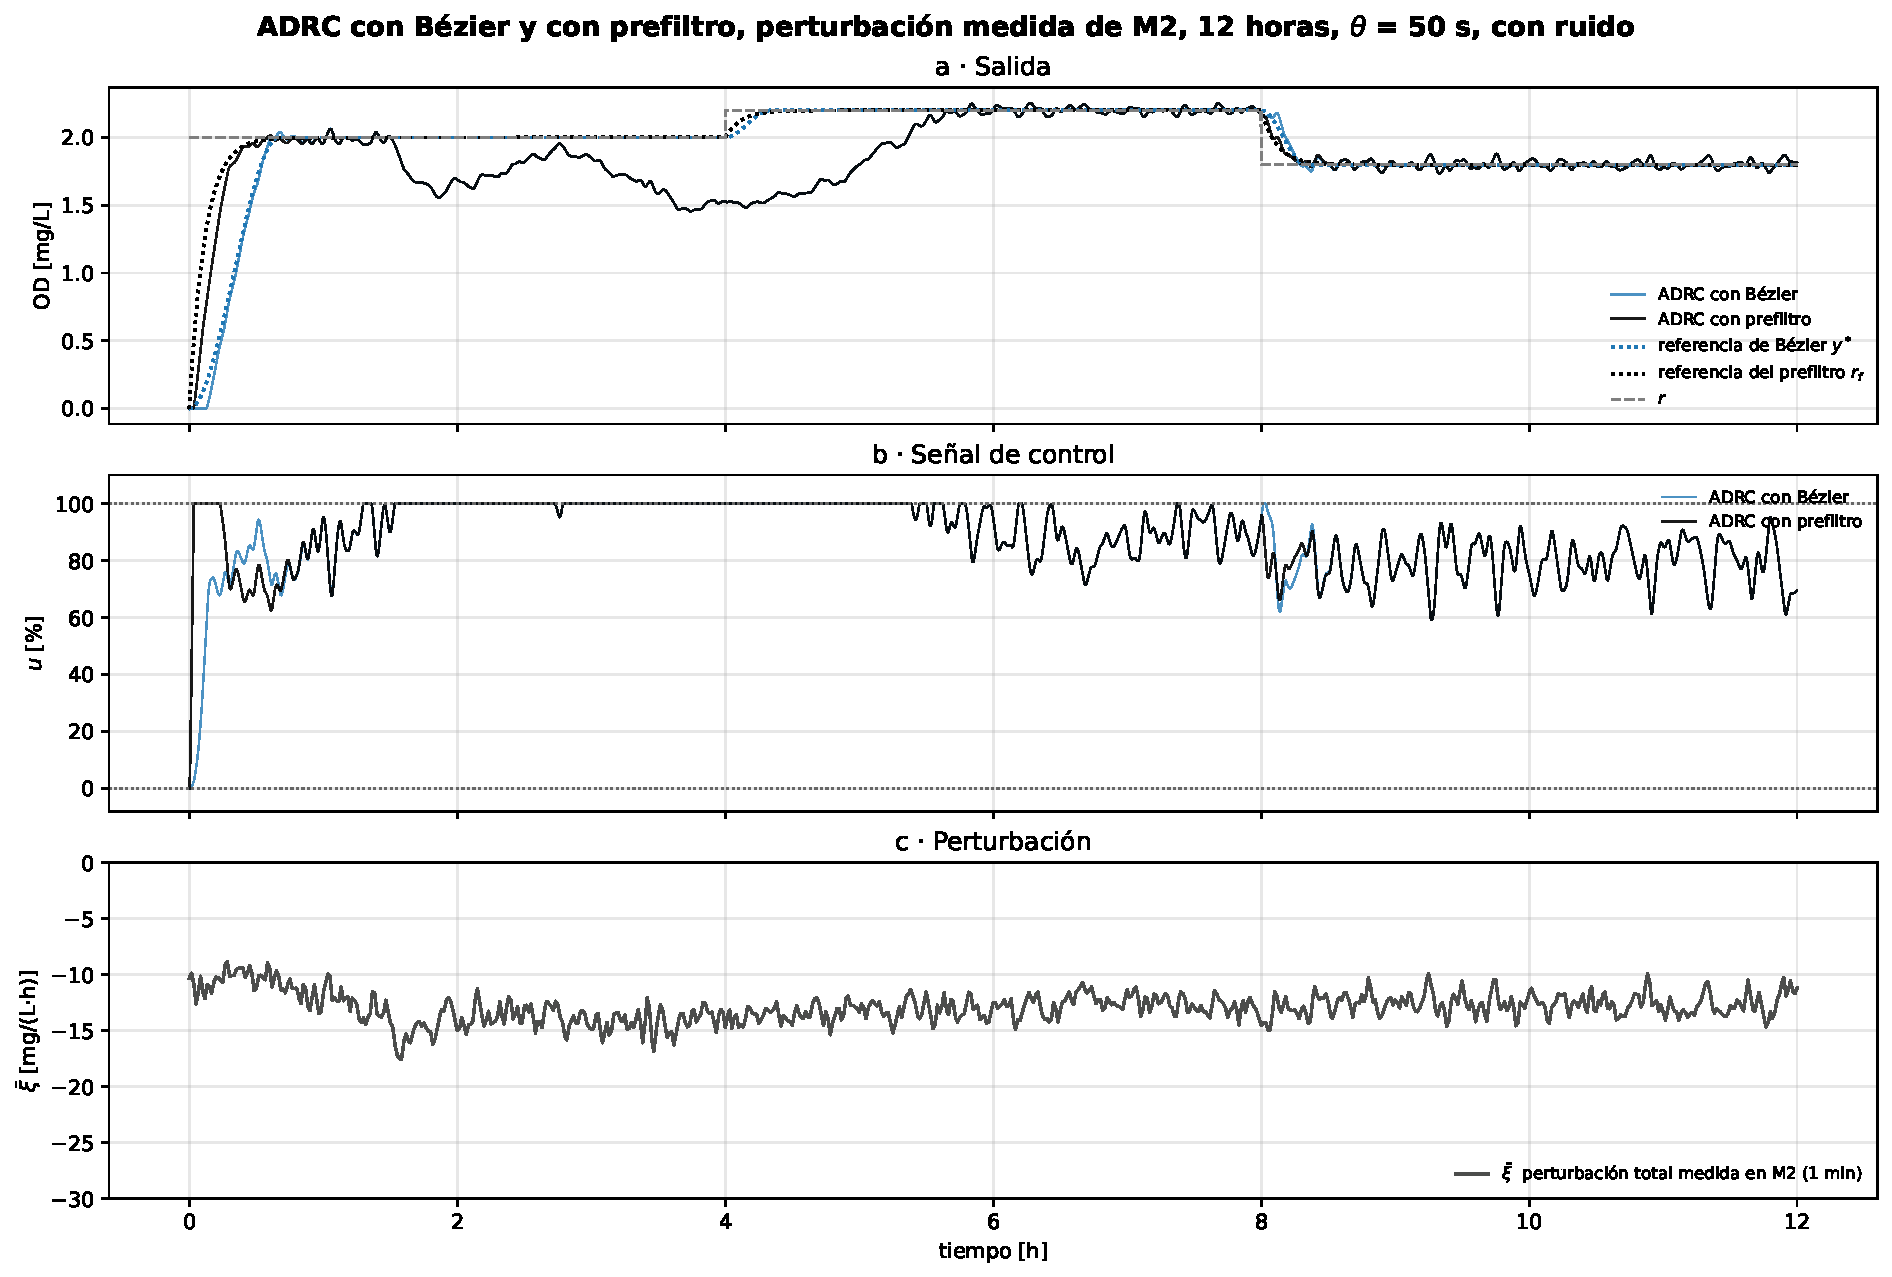
\includegraphics[width=\textwidth]{adrc_acond_perturbacion.pdf}
  \caption[ADRC con Bézier y con prefiltro, con la perturbación medida]{ADRC con la referencia
    acondicionada por la curva de Bézier y por el prefiltro, con la misma perturbación medida,
    consignas, retardo y ruido de la Figura~\ref{fig:pid_adrc_perturbacion}. (a) Salida, con la referencia
    de Bézier y la del prefiltro en punteado. (b) Señal de
    control. (c) Perturbación total sobre la salida $\bar{\xi}$, medida.}
  \label{fig:adrc_acond_perturbacion}
\end{figure}

%--------------------------------------------------------------------
\section{Comparación de desempeños}
\label{sec:pid_mejores}

Con el mismo procedimiento de sintonía se puede obtener un controlador con mejor desempeño que el
ADRC, sin que la señal de control llegue al $100~\%$ (Figura~\ref{fig:pid_mejores},
Tabla~\ref{tab:pid_mejores}): un PI ($T_d = 0$), sintonizado de forma muy similar al PID. Primero se
ajusta $K_p$ para que el salto inicial no supere el $40~\%$; como el PI no tiene derivada, todo el salto
es proporcional y queda $K_p = 200~\%/(\mathrm{mg/L})$. Luego se ajusta $T_i$ para que tenga la misma
robustez que el ADRC, en este caso el mismo margen de fase sin retardo, $65{,}8^{\circ}$, porque con la
misma $M_s$ queda casi inestable con retardo. Resulta
$T_i = 188$~s. Con más o menos la misma robustez, este PI sigue la consigna casi igual que el ADRC y
rechaza mejor la perturbación; ahora bien, sin retardo sigue teniendo un mayor sobrepico. Aun así, para
este tipo de plantas de primer orden, un PI solo puede ser incluso mejor que un PID. En la
Figura~\ref{fig:pid_mejores_sensibilidad} se ve por qué: el PI atenúa más las perturbaciones de baja
frecuencia y, con retardo, su pico de sensibilidad es menor que el del ADRC, a cambio de dejar pasar más
ruido.

\begin{figure}[H]
  \centering
  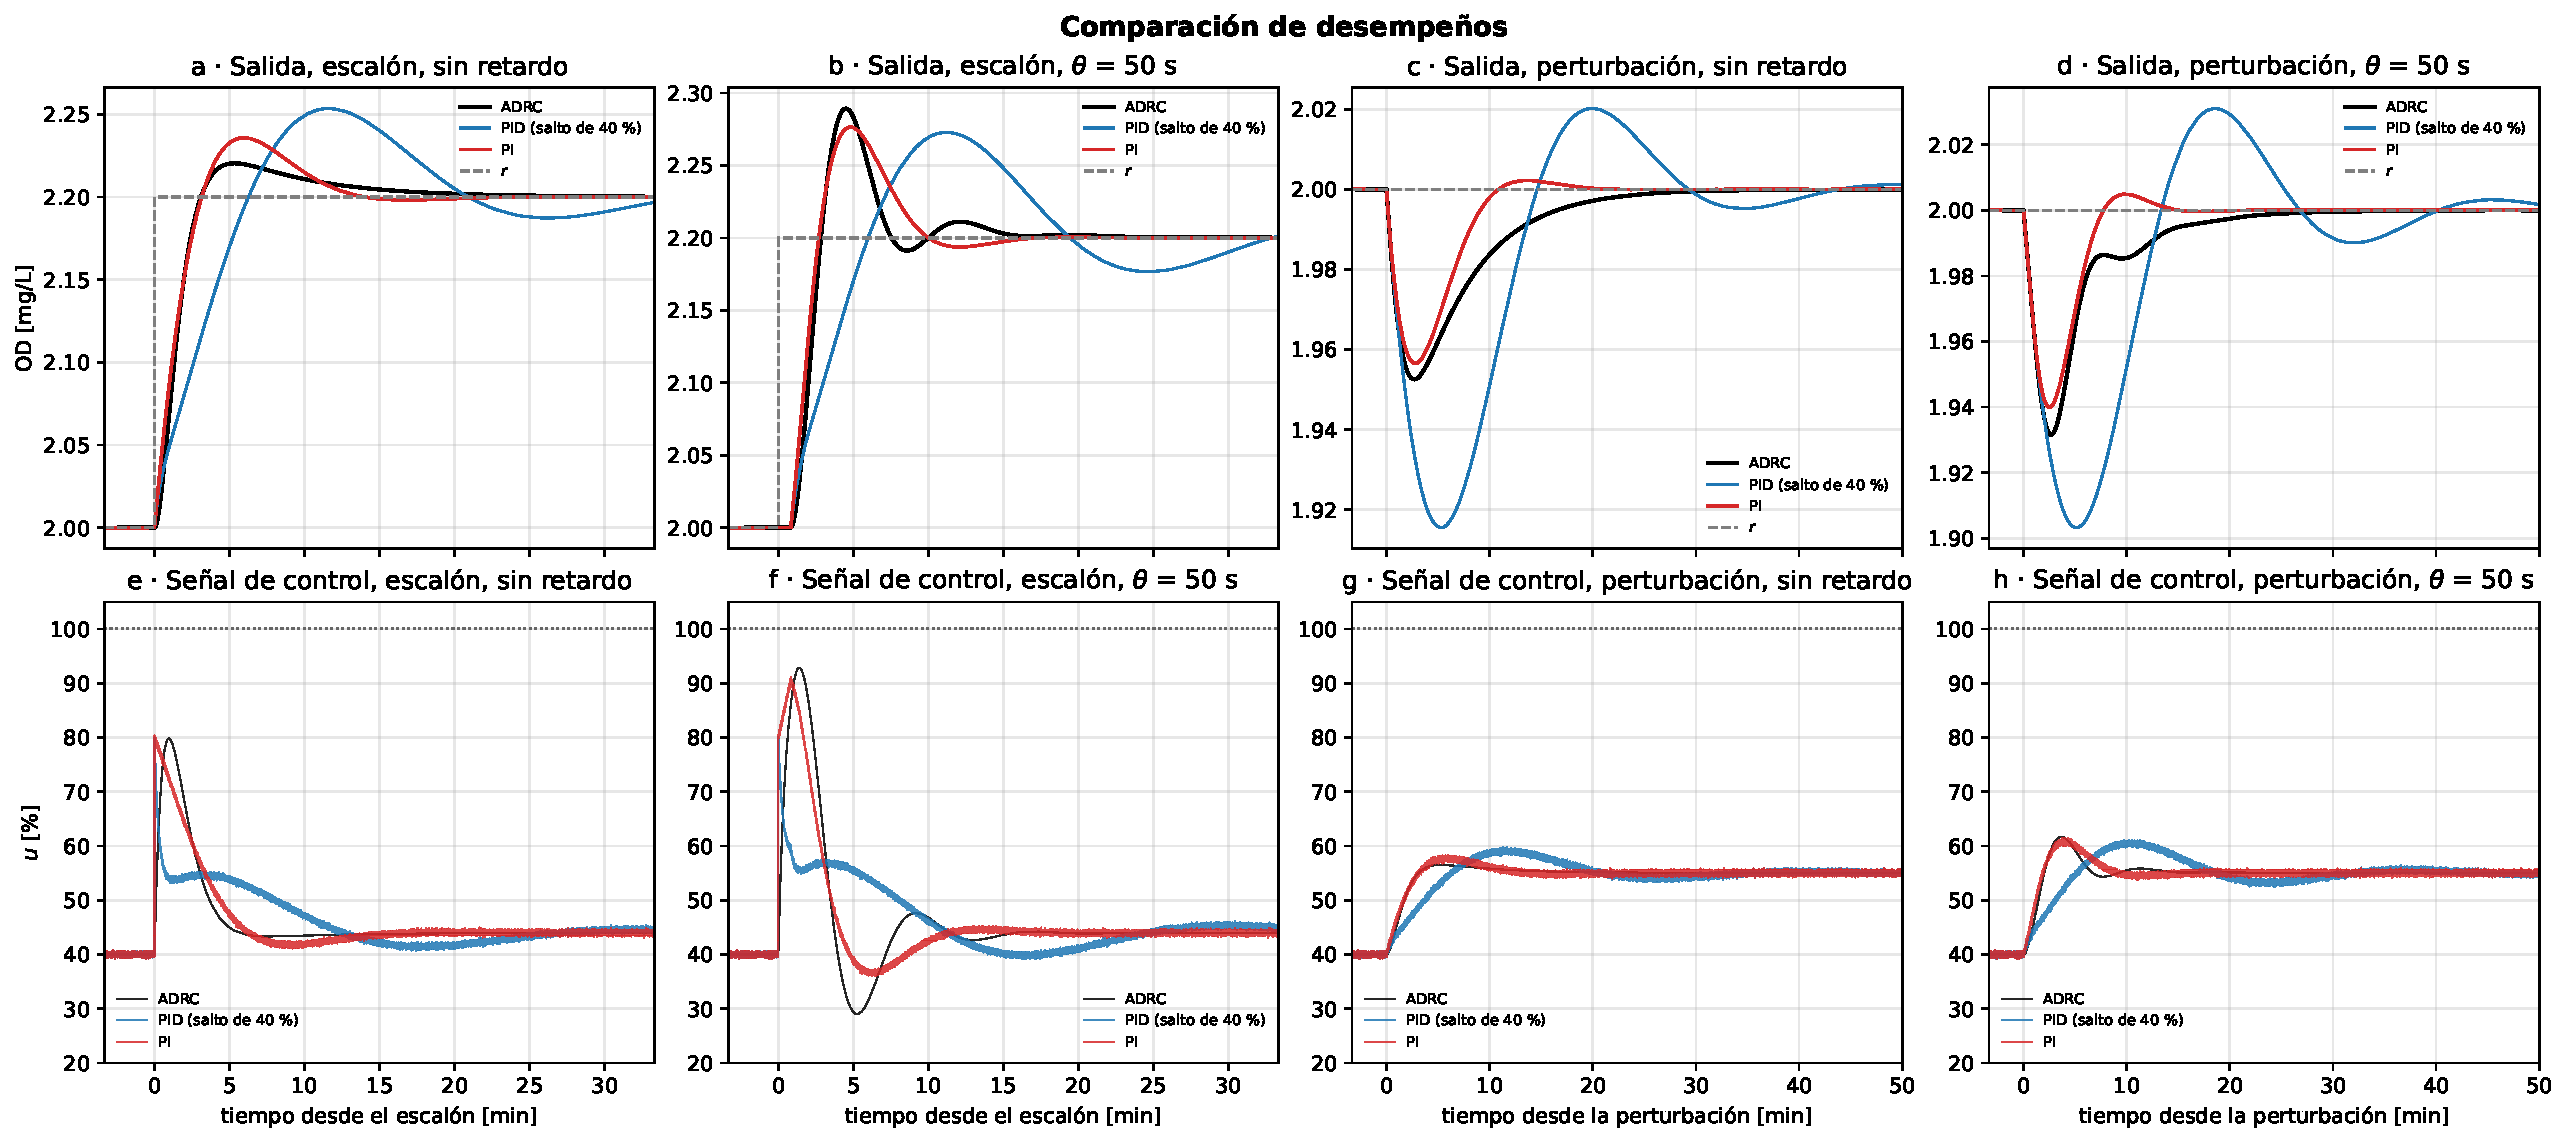
\includegraphics[width=\textwidth]{pid_mejores.pdf}
  \caption[Comparación de desempeños]{ADRC, PID \eqref{eq:pid_ganancias} y PI
    ($K_p = 200~\%/(\mathrm{mg/L})$, $T_i = 188$~s), con el ruido del sensor y
    el soplador limitado entre $0$ y $100~\%$. (a), (b), (e) y (f) Escalón de consigna de $2{,}0$ a
    $2{,}2$~mg/L; (c), (d), (g) y (h) perturbación de entrada $\varepsilon = -15~\%$. En cada par, sin retardo
    y con $\theta = 50$~s; arriba, la salida, y abajo, la señal de control.}
  \label{fig:pid_mejores}
\end{figure}

\begin{table}[H]
\centering
\caption[Robustez y desempeño en la comparación de desempeños]{Robustez y desempeño del ADRC, el PID y el
  PI, sin retardo y con $\theta = 50$~s (Tabla~\ref{tab:metricas}). Los
  índices se miden sin ruido, salvo $\sigma_u$.}
\label{tab:pid_mejores}
\renewcommand{\arraystretch}{1.3}
\resizebox{\textwidth}{!}{%
\begin{tabular}{lcccccccc}
\toprule
 & $\boldsymbol{M_s}$ & \textbf{MF} & \textbf{IAE consigna} & \textbf{ITAE consigna} & $\boldsymbol{M_p}$ & \textbf{IAE rechazo} & $\boldsymbol{u_{\max}}$ & $\boldsymbol{\sigma_u}$ \\
 & $\theta = 0$ / $50$~s & $\theta = 0$ / $50$~s & [mg$\cdot$s/L] & [mg$\cdot$s$^2$/L] & [\%] & [mg$\cdot$s/L] & [\%] & [\%] \\
\midrule
ADRC            & 1,20 / 2,32 & $65{,}8^{\circ}$ / $36{,}0^{\circ}$ & 26,9 / 42,7 & 6\,909 / 9\,308   & 10,2 / 44,6 & 24,8 / 24,8 & 80 / 93  & 0,009 \\
PID             & 1,20 / 1,59 & $50{,}0^{\circ}$ / $37{,}5^{\circ}$ & 69,2 / 88,4 & 40\,127 / 56\,567 & 26,7 / 36,4 & 58,8 / 70,2 & 80 / 80  & 0,220 \\
PI              & 1,00 / 1,73 & $65{,}8^{\circ}$ / $38{,}6^{\circ}$ & 28,3 / 41,0 & 6\,802 / 8\,665   & 17,9 / 38,2 & 15,6 / 16,5 & 80 / 91  & 0,220 \\
\bottomrule
\end{tabular}%
}
\end{table}

\begin{figure}[H]
  \centering
  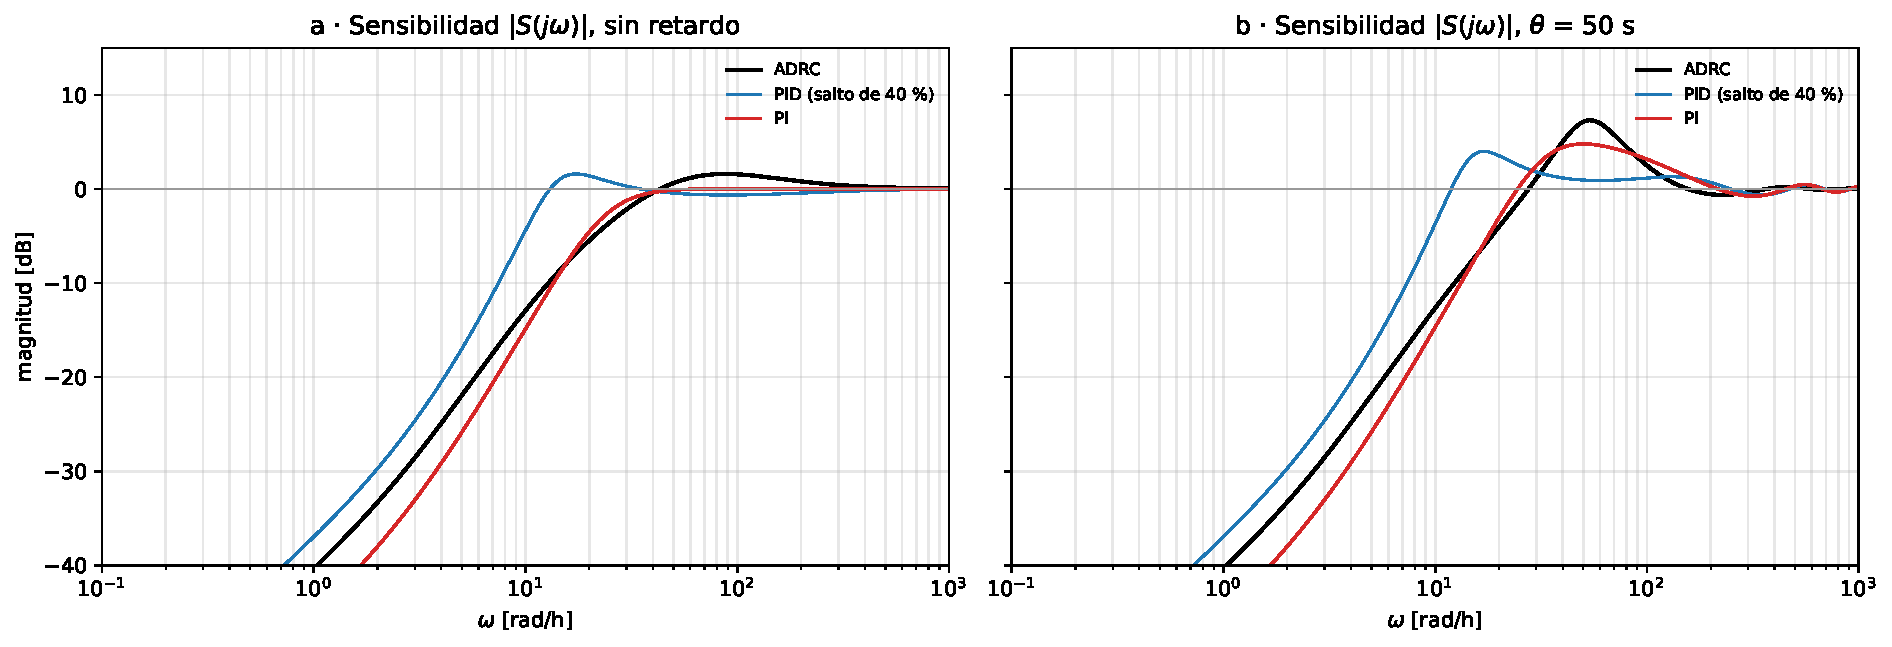
\includegraphics[width=\textwidth]{pid_mejores_sensibilidad.pdf}
  \caption[Sensibilidad en la comparación de desempeños]{Sensibilidad $|S(j\omega)|$ del ADRC, el PID y el
    PI: (a) sin retardo y (b) con $\theta = 50$~s.}
  \label{fig:pid_mejores_sensibilidad}
\end{figure}

Ahora bien, al introducir el retardo se ve que todos tienen más o menos el mismo margen de fase, y el
del ADRC es el más bajo, con $36{,}0^{\circ}$ (Tabla~\ref{tab:pid_mejores}). Pero el ADRC tiene un mejor
comportamiento al arrancar la señal de control, porque la sube de forma
suave, sin el salto del PI ni del PID en el cambio de consigna (Figura~\ref{fig:pid_mejores}(e) y (f)).
Y en el ruido, el ADRC casi no lo deja pasar, mientras que el PI y el PID sí
(Figura~\ref{fig:pid_mejores}(e) a (h)). La diferencia entre este ADRC y el PI está en su filtro en
cascada: el ADRC se puede escribir como un PI con un filtro del error \eqref{eq:gpi_pi_filtro}, y es ese
filtro el que no deja pasar el ruido. Además, el ADRC puede llegar a superarlo en seguimiento cuando la referencia es de mayor orden:
con solo subir el grado del modelo de la perturbación se sigue mejor, tanto con el ESO como con el GPI
(Tabla~\ref{tab:gpi_conteo}), y conceptualmente es más simple. 
% ============================================================================
%  Capítulo 7 — Discusión
% ============================================================================
\chapter{Discusión}
\label{cap:discusion}

\section{Interpretación de los hallazgos}
\label{sec:hipotesis_discusion}

\paragraph{Dinámica de la planta.} Al variar el $b_0$ del controlador entre $1/6$ y $6$ veces el
nominal, se evidencia que el lazo de control es capaz de soportar las discrepancias entre las
ganancias (Figuras~\ref{fig:adrc_variacion}(d) y \ref{fig:sat_adrc_gpi_variacion}(d)) sin entrar en
inestabilidad. Por lo que, incluso sin una ganancia exacta, el sistema de control por sí solo tiene
la suficiente robustez para seguir funcionando a pesar de las discrepancias que haya con la planta.
Ahora bien, esto es sin retardo, donde el margen de ganancia es infinito
(Figura~\ref{fig:adrc_rlocus_b0}(a)). Con $\theta = 50$~s el margen de ganancia es de $2{,}12$
(Figura~\ref{fig:adrc_margenes_retardo}), así que el lazo se vuelve inestable si el $b_0$ del
controlador queda por debajo de $b_{0,\mathrm{planta}}/2{,}12$ (Figura~\ref{fig:adrc_rlocus_b0}(b)). Por
eso, si hay duda, conviene que $b_0$ quede por encima del de la planta: el lazo pierde velocidad, pero no
robustez.

\paragraph{Retardo.} El sistema es capaz de aguantar las variaciones del retardo de la planta,
incluso hasta el doble del de diseño, $\theta = 100$~s, sin desestabilizarse
(Figura~\ref{fig:sat_adrc_gpi_variacion}(c)). La cuestión es que se ve un incremento en el sobrepico
y mayores oscilaciones ante una referencia tipo paso: con $\theta = 50$~s el margen de fase baja de
$65{,}8^{\circ}$ a $36{,}0^{\circ}$ (Figura~\ref{fig:adrc_margenes_retardo}), y recordemos que el
margen de fase se puede relacionar con el comportamiento transitorio de un sistema, más
específicamente con su coeficiente de amortiguamiento. Pero en las
Figuras~\ref{fig:adrc_bezier_retardo} y \ref{fig:pref_escalon}, con Bézier y con prefiltro, se observa
cómo el sobrepico casi desaparece: con el prefiltro y $\theta = 50$~s baja de $46$ a $0~\%$, y con
Bézier las respuestas de $\theta = 20$ a $60$~s prácticamente se superponen. El margen de fase del
lazo no cambia, lo que cambia es que la referencia ya no excita esa oscilación, por lo que el sistema
puede responder mucho mejor ante estas discrepancias con los datos de la planta, específicamente con
el retardo.

Ahora bien, para el retardo no sirve aumentar la relación $\omega_o/\omega_c$ subiendo $\omega_o$. En la
Figura~\ref{fig:adrc_margen_fase_kESO}(a) y (c) el margen de fase sube un poco con esa relación, pero eso es
sin retardo. El cruce de ganancia se mueve más rápido, de $37{,}5$ a $66{,}9$~rad/h con
$\omega_o = 10\,\omega_c$, por lo que el retardo máximo \eqref{eq:mapa_robustez} baja de $110$ a
$65$~s, y con $\omega_o/\omega_c \approx 14$ ya queda por debajo de los $50$~s
(Tabla~\ref{tab:adrc_frecuencia_kESO}). Es decir, si el retardo empieza a afectar el sistema, lo que
hay que hacer es bajar $\omega_o$, no subirlo: con $\omega_o/2$ ($\omega_o/\omega_c = 2{,}5$) se llega a $180$~s. Bajar
$\omega_c$ también sirve, porque el cruce casi no se mueve: con $\omega_c/4$ se llega a $154$~s
(Tabla~\ref{tab:adrc_frecuencia_kESO}).
La otra opción, si el retardo se conoce, es sincronizar el observador \eqref{eq:disc_retardo}: con
$\theta = 50$~s el pico de oxígeno baja y se comienza a comportar mejor. 

\paragraph{Manejo de la saturación.} Los esquemas de manejo de la saturación, el del ESO
(Figura~\ref{fig:simulink_eso}, con resultados en la Figura~\ref{fig:adrc_lazo_cerrado_saturacion}) y
el del GPI (Figura~\ref{fig:simulink_gpi}, con resultados en la Figura~\ref{fig:sat_arranque}),
muestran muy buenos resultados: prácticamente logran manejar la saturación y el lazo no se
desestabiliza, incluso ante variaciones de los parámetros de la planta
(Figura~\ref{fig:sat_adrc_gpi_variacion}). Cuando el sistema se satura y regresa no se observa
sobrepico y se mantiene en el régimen de operación presentado en el diseño. En caso contrario, cuando
no hay manejo de saturación, el controlador se demora más en responder después de salir de saturación
y muestra sobrepicos más grandes: en la Figura~\ref{fig:sat_arranque} el GPI sin \emph{anti-windup} se
queda unos $16$~min en $100~\%$ y el oxígeno sube hasta $2{,}79$~mg/L. Lo que ningún esquema evita es
que, mientras el soplador está en el límite, el oxígeno suba más despacio que en el diseño: tarda
$354$~s en alcanzar el $63~\%$ del escalón, frente a $98$~s sin saturación.

\paragraph{Manejo del ruido.} Para estos controladores con enfoque de rechazo de perturbaciones se
tiene un manejo del ruido muy adecuado, ya que, como se ha venido mencionando, la función de
transferencia del ADRC basado en ESO es estrictamente propia \eqref{eq:gpi_pi_filtro}. Como se mostró
en la Sección~\ref{sec:impl_ruido}, con \eqref{eq:ruido_ft}, se pueden ajustar las frecuencias que se
desean filtrar y las que se desean estimar a partir de las ganancias del controlador, más
específicamente del ancho de banda del observador. Por lo que el ruido, junto con el retardo, es
quien realmente pone la cota superior a las ganancias del observador. Además, en la
Figura~\ref{fig:adrc_gang_kESO}(h) se ve la función de transferencia del ruido a $u$, y podemos
manejar qué tanto deja pasar el controlador al variar la relación $\omega_o/\omega_c$: entre más
grande, más ruido dejamos pasar, $10{,}5$~dB en alta frecuencia con $\omega_o = 5\,\omega_c$ y
$21{,}2$~dB con $10\,\omega_c$ (Tabla~\ref{tab:adrc_frecuencia_kESO}). Por eso el ancho de banda del
observador tampoco lo debemos dejar tan grande.

\paragraph{Discretización.} Con $T_s = 50$~ms todos los métodos, ya sea ZOH, Tustin, Euler hacia
adelante o Euler hacia atrás, dan una muy buena discretización
(Figura~\ref{fig:disc_metodos_bode}), porque la frecuencia de muestreo está muy por encima de la del
lazo cerrado. A medida que esa frecuencia baja, los métodos sí se empiezan a separar: con $10$ veces
el ancho de banda del lazo cerrado, $T_s = 40$~s, las magnitudes siguen juntas, pero en la fase, en el
cruce de ganancia, Tustin se separa del continuo $0{,}13^{\circ}$, Euler $1^{\circ}$ a $3^{\circ}$ y
ZOH casi $17^{\circ}$ (Figura~\ref{fig:disc_metodos_bode_40}). Por lo que $10$ veces es un mínimo,
y entre mayor sea la frecuencia mejores son los resultados, como se ve en la dinámica de la
Figura~\ref{fig:adrc_discreto_lazo_cerrado}.

Para el caso del ADRC basado en observador de estado extendido, debido a la relación que hay entre
las ganancias del observador $\mathbf{L}$, las del control $\mathbf{K}_p$ y los anchos de banda del
controlador y del observador, se puede ajustar su dinámica fácilmente, solo con pasar esos anchos de
banda al plano $z$ \eqref{eq:disc_ganancias_wc_wo}, por su relación con las ganancias y con la
ubicación de los polos tanto del control como del observador.

\paragraph{Rechazo de perturbaciones.} Viendo los resultados de la Figura~\ref{fig:gpi_sensibilidad},
correspondiente al Bode de la sensibilidad en lazo cerrado del GPI, vemos que podemos ajustar el
rechazo con cada ganancia (Tabla~\ref{tab:gpi_frecuencia}). A baja frecuencia,
$S_{\xi}(s) \approx (k_2/k_0)\,s$ \eqref{eq:gpi_caso_S_asintotas}, por lo que la parte lenta de la
perturbación la deciden $k_2$ y $k_0$: duplicar $k_0$ deja $k_2/k_0$ en la mitad, pero el margen de
fase baja de $65{,}8^{\circ}$ a $54{,}2^{\circ}$. El pico de $|S_{\xi}|$ lo baja sobre todo $k_1$: al
duplicarlo pasa de $40{,}3$ a $34{,}6$~dB, pero el retardo máximo baja de $110$ a $57$~s. Es decir,
lo que se gana en rechazo se paga en robustez, igual que con $\omega_o$ en el ADRC. Con la sintonía
nominal, el pico de $|S_{\xi}|$ queda en $22{,}6$~rad/h, por encima de los $12$~rad/h bajo los que está el
$95~\%$ de la energía de $\bar{\xi}$ (Tabla~\ref{tab:ident_espectro_f}), y una perturbación de $-15~\%$ baja
el oxígeno de $2{,}2$ a $2{,}15$~mg/L sin retardo y a $2{,}13$~mg/L con $\theta = 50$~s
(Figura~\ref{fig:pref_escalon}).

\paragraph{Implementaciones.} En la implementación se obtuvieron buenos resultados, logrando utilizar
un controlador de rechazo activo de perturbaciones en su forma de observador de estado y en su forma
GPI, junto con adecuaciones para su implementación, para una planta $n = 1$ y $m = 1$, por lo que
está diseñado para seguir y rechazar señales tipo paso otorgando la dinámica de una planta de orden
1. El lenguaje que se utilizó fue texto estructurado, uno de los más comunes dentro de la norma
IEC~61131-3, porque de todos es el más cercano a C. Ahora bien, a la hora de implementar, sin importar
el PLC, la marca o el lenguaje, siempre que estén dentro de la norma, se pueden llegar a implementar
estos tipos de controladores sin problemas. Solo es necesario utilizar los esquemas de las
Figuras~\ref{fig:adrc_discreto_retardos} y \ref{fig:disc_formas_directas}, que ya están en retardos,
y cualquier lenguaje de la norma, ya sea Grafcet, ladder, bloques o texto estructurado, tiene dentro
de su especificación formas de representar un retardo y hacer operaciones algebraicas. Para el ESO son
suficientes dos retardos y tres sumas, y para el GPI discreto seis retardos y un bloque de suma
(Figura~\ref{fig:disc_formas_directas}). Por lo que con cualquier enfoque se puede implementar un ADRC y con
cualquier lenguaje se pueden realizar estos retardos sin dificultad, es decir, es multiplataforma.

\paragraph{ADRC con ESO y GPI.} Al comparar los controladores con enfoque de rechazo activo de
perturbaciones, ya sea utilizando un ESO o el GPI, se ve que tienen una relación directa. En el caso
del observador de estado extendido se busca estimar la perturbación y el error de seguimiento mediante
el observador, y el GPI trata de realizar la misma idea bajo reconstrucciones de la señal, a partir de
integraciones de la señal de control y del error \eqref{eq:gpi_integrales}. Todo esto indica que son
estructuras equivalentes que tratan de realizar la misma tarea bajo enfoques diferentes. Con las
ganancias $k_0$, $k_1$ y $k_2$ queda más fácil interpretar cómo es la sensibilidad del rechazo de
perturbaciones en lazo cerrado (Figura~\ref{fig:gpi_sensibilidad}) y cómo cada ganancia puede ayudar a
modificar este efecto en el lazo, además de saber cómo afecta cada parámetro el sobrepico o el tiempo
de asentamiento (Tabla~\ref{tab:gpi_transitorio}). Mientras que el ADRC con ESO ayuda a interpretar el
rechazo activo de perturbaciones por medio de anchos de banda, donde puedo interpretar qué polos están
dedicados al rechazo y qué polos están dedicados al control y a la respuesta transitoria
\eqref{eq:sintonia_polos}.

Además, el polinomio de la sensibilidad en lazo cerrado, $e_y/\xi$, corresponde a los polos del
controlador y del observador juntos \eqref{eq:gpi_producto_S}. Por lo que vamos a tener la misma
sensibilidad, las mismas funciones de transferencia (Figura~\ref{fig:adrc_gang_kESO}), los mismos
márgenes de fase y de ganancia y los mismos anchos de banda, y lo que realmente cambia entre los
esquemas es la forma de sintonizar y su esquema de saturación. Pero incluso ahí se puede pasar de un
esquema a otro y tener el mismo resultado: con $E_1(s) = (s + \omega_o)^2$ \eqref{eq:aw_gpi_wo} el GPI
se comporta igual que el ADRC también cuando satura (Figuras~\ref{fig:sat_arranque} y
\ref{fig:gpi_discreto_vs_adrc}).

\paragraph{Comparación con el PID}
\label{sec:por_que}

Ahora bien, el ADRC también se puede escribir de una forma relacionada con el PID. En la literatura un
ADRC se puede escribir como un PID con un filtro del error, así como en este caso un PI con filtro del
error \eqref{eq:gpi_pi_filtro}. Pero su diferencia con el PID ISA con filtro en la derivada radica en
que la función de transferencia de ese PID es bipropia, y la del ADRC estrictamente propia. Esa es una
primera diferencia, donde el PID tiene peores resultados en su manejo del ruido: como vimos en la
Sección~\ref{sec:impl_ruido}, al ser bipropio deja pasar el ruido hacia la señal de control, con
$\sigma_u$ de $0{,}22~\%$ frente a $0{,}009~\%$ del ADRC (Tabla~\ref{tab:pid_escalon}), haciendo mayor
desgaste en los actuadores, a pesar de que la misma planta se comporte como un filtro.

Ahora bien, el PID se sintonizó para que su señal de control no salte más que la del ADRC y con la
misma sensibilidad máxima sin retardo, y aun así queda por detrás: es más lento, se pasa más en los
cambios de consigna y rechaza peor las perturbaciones (Tablas~\ref{tab:pid_escalon}
y \ref{tab:pid_pert_escalon}). En el PID una sola ganancia fija el rechazo, el
esfuerzo inicial y el ruido, mientras que en el ADRC el rechazo lo pone el observador. Para una planta
de primer orden como esta, un PI sintonizado con el mismo procedimiento y el mismo margen de fase del
ADRC lo supera en rechazo (Figura~\ref{fig:pid_mejores}); lo que el ADRC sigue ganando es una señal de
control que arranca suave y casi sin ruido, y la posibilidad de subir el grado del modelo de la
perturbación sin cambiar su estructura. Además, su enfoque es mucho más práctico: el seguimiento y el
rechazo se entienden y se sintonizan por separado, con dos anchos de banda, de una forma más sencilla,
simple y coherente que con el PID.

Otra diferencia está en la sintonía. Un PID también admite modificar la dinámica moviendo los polos teniendo un modelo de
la planta, pero sus ganancias $K_p$, $T_i$ y $T_d$ no se relacionan directamente con la dinámica deseada
ni con la perturbación, por lo que la mayoría de las sintonizaciones se hacen en campo, de forma
empírica. El ADRC, en cambio, se puede sintonizar por anchos de banda, para rechazar las perturbaciones
o poder ajustar una dinámica deseada del error, bajo un \emph{pole placement} con las ganancias $k_0$, $k_1$ y $k_2$,
para ajustar la función de sensibilidad en lazo cerrado y rechazar perturbaciones, o en su forma
clásica de PI más filtro.

\section{Limitaciones del estudio}
\label{sec:limitaciones}

\begin{enumerate}
  \item \textbf{No hay trazas de la planta operando con ADRC.} Dados los tiempos y las restricciones,
  es complicado tener una ventana de tiempo para realizar la implementación del código en campo dentro
  de las fechas admisibles para el proyecto. Por eso la validación es en simulación, con la planta
  identificada y la perturbación sintetizada de sus datos, y se deja todo el proyecto probado y
  verificado para su puesta en marcha cuando se tenga el espacio en campo para instalarlo.

  \item \textbf{El retardo está acotado, no medido con precisión.} El retardo se encuentra acotado y
  obtenido visualmente a partir de una de las pruebas de uno de los tres módulos dispuestos en la
  planta, por lo que dependiendo del módulo puede variar. Lo positivo de esto es que se evaluó el
  retardo con diferentes variaciones y el controlador logró responder adecuadamente, incluso mejor con
  los acondicionamientos que se hicieron.

  \item \textbf{Las variaciones se probaron una a la vez.} En las
  Figuras~\ref{fig:adrc_variacion} y \ref{fig:sat_adrc_gpi_variacion} se cambia un parámetro de la
  planta a la vez, por lo que no todas las combinaciones quedan cubiertas, y solo se validan las
  más importantes, como $b_0$ y $\theta$. Pueden aparecer casos en los que, al variar dos
  parámetros a la vez, se tengan más restricciones. Por ejemplo, si se tiene $\theta = 50$~s y al
  mismo tiempo $b_{0,\mathrm{planta}} = 0{,}327$~mg/(L$\cdot$h$\cdot$\%), un caso extremo, se tendría
  $b_{0,\mathrm{planta}}/b_0 = 2{,}18$, que supera el margen de ganancia de $2{,}12$, y el lazo
  quedaría inestable. En ese caso habría que reajustar las ganancias para aumentar el margen de
  fase y que el lazo soporte más retardo, además de suavizar la referencia con el prefiltro o con
  Bézier para disminuir el sobrepico ante el escalón. De igual forma, se recomienda que el retardo
  no sea muy alto; si lo es, toca resintonizar y, si se puede, sincronizar el observador.


  \item \textbf{Limitación del orden de la perturbación.} Se escogió para el diseño una perturbación de
  orden $m = 1$, un solo integrador, por lo que al cambiar la referencia por rampas u otros tipos se
  tendrán errores de seguimiento, relativamente pequeños en función de las ganancias de los
  controladores, pero de igual forma existirá el error de seguimiento. Para estos entornos industriales
  donde se usan PID no es tanto problema, pero si llegado el caso se necesita seguir otro tipo de
  referencias de forma exacta, $e_y(\infty) = 0$, deberá modificarse cada uno de los bloques de los
  controladores implementados y diseñados en este documento.
\end{enumerate}

\section{Implicaciones prácticas}
\label{sec:implicaciones}

Para quien tenga que decidir sobre un lazo de oxígeno en servicio, los
resultados se traducen en cinco recomendaciones concretas:

\begin{enumerate}
  \item \textbf{Medir $\bo$ en las unidades del bloque, no en unidades
  físicas.} Un solo escalón registrado a la velocidad del PLC basta, y evita
  toda la cadena de conversiones --- consigna a potencia, potencia a caudal de
  aire --- que es donde se acumula el error. Además, la ganancia se debe obtener
  siempre cerca al punto de operación, y tratar de llegar a él posteriormente con
  algún método que acondicione la referencia.

  \item \textbf{Dejar $\bo$ por encima del de la planta si hay duda.} Con $b_0$ sobreestimado la respuesta es
  más lenta, pero se conserva la robustez. Con $b_0$ subestimado el controlador es más agresivo y con
  retardo el lazo se acerca al límite de inestabilidad (Figura~\ref{fig:adrc_rlocus_b0}).

  \item \textbf{Elegir $\wo$ con el espectro de la perturbación y el ruido de
  la sonda.} Se elige como un factor de $\wc$, por encima de donde está la energía de la perturbación,
  pero sin dejar pasar el ruido de la sonda, o no lo filtraremos y tendremos una señal de control
  ruidosa. Cuando se tengan problemas de ruido, incluso es más fácil cambiar el instrumento o hacer
  mejores acondicionamientos en campo que realizar un sobreajuste en el observador.

  \item \textbf{Entregar la orden aplicada y acondicionar la referencia.} Al observador le debe entrar
  $u_{\mathrm{sat}}$ y no $u$, y los cambios de consigna deben pasar por Bézier o por el prefiltro, que
  no cambian el rechazo de perturbaciones y bajan el pico de $u$, de $93$ a $54~\%$ con
  $\theta = 50$~s (Figura~\ref{fig:pref_escalon}).

  \item \textbf{Migrar progresivamente.} Se puede arrancar el control con anchos de banda conservadores,
  no muy grandes, y dependiendo de su comportamiento en el transitorio y en el rechazo ir variando las
  ganancias, siguiendo el resumen de la Sección~\ref{sec:impl_resumen} para obtener buenos resultados.
  Como el bloque recibe las mismas señales que el PID, es una ruta de puesta en marcha que no requiere
  detener el proceso ni convencer a nadie de antemano.
\end{enumerate}

% ============================================================================
%  Capítulo 8 — Conclusiones
% ============================================================================
\chapter{Conclusiones}
\label{cap:conclusiones}

\section{Conclusiones por objetivo}

\textbf{OE1 --- Caracterizar las perturbaciones.} Las perturbaciones del lazo
de oxígeno quedaron cuantificadas sobre 22 meses de operación
(Tabla~\ref{tab:ident_resumen}) y llevadas con \eqref{eq:pid_eps} a la unidad que decide el diseño,
\% de la señal de control. Con ellas se generó la perturbación sintética
(Figura~\ref{fig:ident_perturbacion}) con la que se validaron los controladores implementados, y en la
Figura~\ref{fig:pid_adrc_perturbacion} se ve que durante las 12~h el observador sigue la perturbación
aplicada. El $95~\%$ de su energía está por debajo de $12$~rad/h y el $99~\%$ por debajo de $56$~rad/h
(Tabla~\ref{tab:ident_espectro_f}), que es lo que orientó el ancho de banda del observador.

\textbf{OE2 --- Diseñar un GPI robusto sobre el error.} El controlador GPI de
orden $n=1$, $m=1$ quedó diseñado, discretizado y dotado de un esquema de
\emph{anti-windup} deducido de sus propias ganancias. El esquema elimina el sobrepaso por saturación:
en el arranque, sin él el oxígeno sube hasta $2{,}79$~mg/L, y con él llega a la consigna sin pasarse
(Figura~\ref{fig:sat_arranque}). Se verificó que su diseño en tiempo continuo coincide con su
realización en discreto (Figura~\ref{fig:gpi_discreto_vs_adrc}). Además, se implementó en el PLC para
los dos tipos de sintonía, por anchos de banda o por las ganancias $k_0$, $k_1$ y $k_2$,
correspondientes a las de un PI con filtro del error \eqref{eq:gpi_pi_filtro}.

\textbf{OE3 --- Diseñar un ADRC basado en ESO sobre el error.} El controlador
quedó diseñado con criterio físico para las dos perillas: $\wc = 4/\tau$, cuatro veces más rápido que
la planta en lazo abierto, y $\wo = 5\,\wc = 60$~rad/h, validado contra el contenido espectral de la
perturbación y con un rechazo coherente con las perturbaciones de orden $m=1$. Con esa sintonía el
margen de fase es de $65{,}8^{\circ}$ sin retardo y de $36{,}0^{\circ}$ con $\theta = 50$~s
(Figuras~\ref{fig:adrc_frecuencia} y \ref{fig:adrc_margenes_retardo}), y el escalón de $2{,}0$ a
$2{,}2$~mg/L se asienta en $15{,}7$~min. Además, se presenta una relación de equivalencia entre el GPI
y el ADRC basado en observador de estado extendido \eqref{eq:eso2gpi}.

\textbf{OE4 --- Metodología de implementación en PLC.} Se documentó una
metodología (Sección~\ref{sec:impl_resumen}), verificada sobre plataformas basadas en CODESYS, con
bloques de función en texto estructurado formulados sobre el error para que
sustituyan al PID existente sin modificar la arquitectura del lazo
(Tablas~\ref{tab:plc_adrc_eso}, \ref{tab:plc_gpi} y \ref{tab:plc_adrc_gpi}, Figura~\ref{fig:plc_codesys}, Anexo~\ref{anx:st}). Los dos
controladores se ejecutaron en las plataformas, lo que valida su funcionamiento junto con los
productos digitales diseñados bajo los aspectos prácticos de implementación, como la curva de Bézier
para la referencia y el prefiltro (Tablas~\ref{tab:plc_prefilter_gpi}, \ref{tab:plc_prefilter_adrc} y \ref{tab:plc_bezier}).

\textbf{OE5 --- Validación frente a un PID convencional.} La validación se hizo en simulación, con la
planta identificada y la perturbación sintetizada de los datos reales, ya que el controlador no se ha
puesto en marcha en campo (Sección~\ref{sec:limitaciones}). La comparación se hizo contra dos
referencias: los arranques medidos del PID real, que unas veces llegan limpios y otras oscilan con
sobreimpulsos de $44$ y $91~\%$ (Figura~\ref{fig:ident_pid}), y un PID ISA sintonizado para que su
señal de control no salte más que la del ADRC en el cambio de consigna y tenga la misma sensibilidad
máxima sin retardo. Con esas condiciones, el ADRC es mejor en el escalón de consigna, con un IAE de
$42{,}7$ frente a $88{,}4$~mg$\cdot$s/L con el retardo de diseño (Tabla~\ref{tab:pid_escalon},
Figura~\ref{fig:pid_adrc_escalon}), y en el rechazo de una perturbación de entrada, que corrige sin
pasarse de la consigna (Tabla~\ref{tab:pid_pert_escalon}). En las 12~h con perturbación sintética el
IAE del ADRC es algo menor, $1{,}86$ frente a $2{,}23$~mg$\cdot$h/L (Sección~\ref{sec:pid_perturbacion}), y
el PID se pasa unas tres veces más en los cambios de consigna y maneja peor el ruido, con una señal de
control más ruidosa ($\sigma_u$ de $0{,}22$ frente a $0{,}009~\%$,
Figura~\ref{fig:pid_adrc_escalon}). El PID solo queda mejor en robustez con retardo, con
$M_s$ de $1{,}59$ frente a $2{,}32$ (Tabla~\ref{tab:pid_robustez}), a cambio de poco más de un tercio
del ancho de banda. Para esta planta de primer orden, un PI con el mismo margen de fase del ADRC puede
superarlo en rechazo (Figura~\ref{fig:pid_mejores}), pero deja pasar mucho más ruido al soplador.

\section{Conclusión general}

Las dos arquitecturas de rechazo activo evaluadas --- GPI y ADRC con ESO ---
son, para este proceso y con las ganancias correspondientes, el mismo
controlador escrito de dos maneras, es decir, son equivalentes. Su ventaja frente al PID no está
estrictamente en el IAE, dado que con diferentes sintonizaciones puedo tener mejores IAE. Bajo la misma
sensibilidad máxima y el mismo esfuerzo inicial, está en el precio que cada uno paga por ese IAE: en
sobrepico, en el rechazo de perturbaciones y en el ruido que llega al soplador. En general, se pudieron validar los controladores y sus respectivas
equivalencias en una problemática industrial donde el PID es la forma habitual de control, y se llegó
a una metodología y a unos aspectos prácticos de implementación para realizar una puesta en marcha
adecuada a cada problemática que pueda llegar a surgir, usando plataformas basadas en CODESYS. Lo que
queda pendiente es confirmarlo en campo.

\section{Aportes principales}

\begin{enumerate}

  \item \textbf{Validación de controladores más que todo teóricos, pero con enfoque industrial.}
  Si bien ya se ha demostrado que estos tipos de controladores avanzados, como el ADRC y el GPI, tienen
  algunas ventajas frente a controladores clásicos como el PID, a nivel de manejo de ruido y de
  facilidad de sintonización relacionada con fenómenos físicos como los anchos de banda de la planta y
  de la perturbación, o incluso por \emph{pole placement}, no son tan vistos en proyectos o procesos
  industriales, donde el PID sigue ganando terreno. Aquí se demuestra una forma más práctica de
  implementarlos, diseñados sobre los datos reales de una planta en operación.

  \item \textbf{La reconstrucción explícita de la equivalencia ESO--GPI.} Se buscaba una forma de
  obtener el mismo resultado bajo dos enfoques diferentes de construcción de controladores, y la
  equivalencia \eqref{eq:eso2gpi} se mantiene en tiempo continuo, en discreto y también con saturación
  (Figuras~\ref{fig:gpi_vs_adrc}, \ref{fig:sat_arranque} y \ref{fig:gpi_discreto_vs_adrc}).

  \item \textbf{Una metodología de implementación en PLC verificada en CODESYS.} Se entregan códigos
  escritos en texto estructurado, correspondiente a la norma IEC~61131-3 (Anexo~\ref{anx:st}), y su
  metodología de sintonización y uso (Sección~\ref{sec:impl_resumen}), por lo que queda listo para que
  cualquier usuario lo pruebe y tenga forma de sintonizarlo fácilmente.

  \item \textbf{Aspectos prácticos de implementación.} Se realizaron diferentes experimentos para
  demarcar qué se debe considerar a la hora de integrar estos tipos de controladores, o en general
  controladores, en entornos industriales, y cómo se puede hacer un mejor uso de ellos con
  acondicionamientos específicos como el manejo de la saturación, una referencia acotada e incluso un
  manejo del ruido, que a nivel industrial puede estar presente en todos los procesos.

\end{enumerate}

\section{Trabajo futuro}

\begin{enumerate}
  \item \textbf{Terminar la puesta en marcha en campo.} Teniendo ya todos los esquemas listos para
  probar, simulados y con sus códigos establecidos, queda su puesta en marcha como pendiente.

  \item \textbf{Evaluar bajo influentes de lluvia, cambios ambientales y zonas muertas de los motores.}
  Si bien ya está validado bajo perturbaciones y sintonización relacionadas con la planta, falta
  validarlo bajo históricos de un tiempo prolongado, de meses, para ver su comportamiento bajo
  condiciones ambientales cambiantes, como tormentas o lluvias, donde se modifica el caudal y cambia la
  biología de la planta. Si bien el controlador responde adecuadamente a perturbaciones supuestas e
  interpretadas de los datos, es necesario realizar pruebas prácticas en las que se involucren mayores
  perturbaciones, y más que todo dirigidas a los actuadores, como cambios en los difusores o en la
  potencia de los mismos motores al cambiar equipos o introducir nuevos, siendo esto evidenciado en un
  cambio de las ganancias, además de la presencia de posibles zonas muertas en los motores.

  \item \textbf{Reducción del esfuerzo de control.} Una de las diferencias entre el esquema basado en el
  error y el esquema de estimación de la señal de salida es que, al introducir la referencia por el
  observador en el error de seguimiento y meter un paso, la acción de control va a ser muy fuerte,
  debido a que el controlador debe compensar la derivada de un paso, que es un impulso,
  $u^* = [y^*]^{(n)}$, y eso genera un enorme esfuerzo de la señal de control. Aquí se redujo con Bézier y
  con el prefiltro; otra forma de reducirlo es mediante un \emph{clutch} que no inyecte directamente todo
  el esfuerzo de la señal de control a la planta, sobre lo que ya existen documentos como
  \cite{quecan2026clutch}.

  \item \textbf{Implementación de controladores ADRC con otro tipo de perturbación.} Poder llevar a
  estructuras implementables en equipos digitales grados mayores de perturbación, para tener mejor
  seguimiento ante otros tipos de señales, como rampas o incluso señales oscilatorias, de las que ya
  existe una teoría grande, y el único esfuerzo es ver la forma de facilitar su implementación.

  \item \textbf{Implementación analógica de controladores en circuitos dedicados.} Si bien la
  discretización ha sido una forma muy buena de implementar diferentes controladores teóricos continuos,
  sería interesante validar estos tipos de controladores en SoC con periféricos totalmente analógicos,
  cuya única función sea realizar el control. Por lo que, bajo un enfoque de diseño ASIC
  (\emph{Application-Specific Integrated Circuit}) mixto, se podría llegar a crear un producto con una
  parte digital que permita la interacción con el usuario y modelar cada una de las ganancias del
  controlador por software, pero con una realización completamente analógica en un chip dedicado.

\end{enumerate}


\cleardoublepage
% ============================================================================
%  Declaración del uso de inteligencia artificial
% ============================================================================
\chapter*{Declaración del uso de inteligencia artificial}
\addcontentsline{toc}{chapter}{Declaración del uso de inteligencia artificial}
\markboth{Declaración del uso de inteligencia artificial}{Declaración del uso de inteligencia artificial}

En el desarrollo de este trabajo se emplearon herramientas de inteligencia
artificial generativa (modelos de lenguaje de gran escala) como asistente de
programación y de redacción. El uso se concentró en:

\begin{itemize}
  \item \textbf{Código de análisis y simulación.} Asistencia en la escritura y
  depuración de los cuadernos de Python y de los módulos de análisis de datos.
  Todos los resultados numéricos fueron ejecutados por el autor y verificados
  contra referencias independientes --- las trazas del PLC y los informes de
  servicio de la planta.
  \item \textbf{Revisión crítica de los análisis.} Contraste de hipótesis
  alternativas, detección de sesgos en los estimadores y verificación de
  consistencia entre documentos intermedios. Varias de las correcciones
  incorporadas en el Capítulo~\ref{cap:caracterizacion} --- en particular la del
  sesgo del estimador y la del diagnóstico por correlación instantánea ---
  surgieron de ese contraste.
  \item \textbf{Redacción y edición.} Asistencia en la organización y la
  redacción del documento en \LaTeX, a partir de material, resultados y
  decisiones del autor.
\end{itemize}

Las siguientes tareas \textbf{no} fueron delegadas: la formulación del
problema y de las hipótesis, la obtención y curaduría de los datos, las
decisiones de diseño de los controladores, la interpretación de los resultados
y las conclusiones. Ninguna cifra, figura o referencia de este documento
procede de una generación no verificada: los datos provienen del historiador
de la planta y de las trazas del PLC, y las referencias bibliográficas fueron
consultadas en su fuente.

El autor asume la responsabilidad plena por el contenido, la exactitud y la
integridad de este trabajo.


\cleardoublepage
\bibliographystyle{IEEEtran}
\bibliography{references}

\appendix
% ============================================================================
%  Anexos
% ============================================================================
% Cambiar aquí la dirección del repositorio
\newcommand{\repourl}{https://github.com/EstebanUnal-Hub/ADRC_WWTP}
\newcommand{\repositorio}{\url{\repourl}}
% enlace a una sección del README: \readme{ancla}{texto}
\newcommand{\readme}[2]{\href{\repourl\##1}{#2}}

\chapter{Repositorio de código y datos}
\label{anx:st}
\label{anx:archivos}

El código, los cuadernos, los datos procesados y los bloques del PLC de este trabajo están en el
repositorio \repositorio, cuyo \href{\repourl}{README} los explica en detalle. La
Tabla~\ref{tab:anx_repo} resume los archivos principales; la última columna enlaza a la sección del
README que explica cada uno.

{\renewcommand{\arraystretch}{1.15}
\begin{longtable}{|>{\footnotesize\raggedright\arraybackslash}p{5.6cm}|>{\small\raggedright\arraybackslash}p{6.9cm}|>{\small\centering\arraybackslash}p{1.9cm}|}
\caption{Archivos principales del repositorio.}
\label{tab:anx_repo} \\
\hline
\rowcolor[gray]{0.9}
\small\textbf{Archivo} & \textbf{Contenido} & \footnotesize\textbf{README} \\ \hline
\endfirsthead
\hline
\rowcolor[gray]{0.9}
\small\textbf{Archivo} & \textbf{Contenido} & \footnotesize\textbf{README} \\ \hline
\endhead
\texttt{README.md} & Descripción general del repositorio y de cada carpeta. & \href{\repourl}{Inicio} \\ \hline
\texttt{Datos/analisis/}\newline\texttt{analisis\_dinamica\_limpio.ipynb} & Identificación de la planta
por ventanas ARX y caracterización con el histórico del SCADA (Capítulo~\ref{cap:caracterizacion}). &
\readme{3-plant-model-and-identification}{Sec. 3} \\ \hline
\texttt{Simulaciones/PTAR/02 Diseño/Python/}\newline\texttt{ADRC\_PTAR\_continuo.ipynb} & ADRC con ESO
y GPI en tiempo continuo: diseño, equivalencia, \emph{anti-windup}, acondicionamiento de la referencia
y comparación con el PID (Capítulos~\ref{cap:ADRC-ESO} a \ref{cap:comparacion_pid}). &
\readme{4-error-based-adrc-with-extended-state-observer}{Sec. 4 a 6} \\ \hline
\texttt{Simulaciones/PTAR/02 Diseño/Python/}\newline\texttt{ADRC\_PTAR\_discreto.ipynb} & ADRC con ESO
y GPI en tiempo discreto: discretización y simulación con retardo
(Sección~\ref{sec:impl_discretizacion}). & \readme{64-discretization}{Sec. 6.4} \\ \hline
\texttt{P\&ID/P\&ID.vsdx} y \texttt{P\&ID.pdf} & Plano de la etapa de aireación, con el lazo 100 de
oxígeno disuelto (Figura~\ref{fig:pid_tikz}). & \readme{2-process-and-control-loop}{Sec. 2} \\ \hline
\texttt{PLC\_ST/Codigos/*.st}\newline\texttt{PLC\_ST/Libreria\_ADRC/} & Los siete bloques de función en
texto estructurado (IEC~61131-3), también documentados como librería de ctrlX
(Sección~\ref{sec:impl_plc}). & \readme{7-plc-implementation}{Sec. 7} \\ \hline
\end{longtable}
}


\end{document}
